% !TEX TS-program = pdflatex
% !TEX encoding = UTF-8 Unicode

% This is a simple template for a LaTeX document using the "article" class.
% See "book", "report", "letter" for other types of document.

\documentclass[11pt]{article} % use larger type; default would be 10pt

%\usepackage[utf8]{inputenc} % set input encoding (not needed with XeLaTeX)

%%% Examples of Article customizations
% These packages are optional, depending whether you want the features they provide.
% See the LaTeX Companion or other references for full information.

%%% PAGE DIMENSIONS

\usepackage{geometry} % to change the page dimensions
\geometry{a4paper} % or letterpaper (US) or a5paper or....
%\geometry{margins=2in} % for example, change the margins to 2 inches all round
% \geometry{landscape} % set up the page for landscape
%   read geometry.pdf for detailed page layout information
\usepackage{fullpage}
%\usepackage[top=tlength, bottom=blength, left=llength, right=rlength]{geometry}
%Edit individual page dimension variables described above, using the \addtolength and \setlength commands. For instance,
%\oddsidemargin=-1cm
%\setlength{\textwidth}{6.5in}
%\addtolength{\voffset}{-5pt}

\usepackage{graphicx} % support the \includegraphics command and options

% \usepackage[parfill]{parskip} % Activate to begin paragraphs with an empty line rather than an indent

%%% PACKAGES
\usepackage{booktabs} % for much better looking tables
\usepackage{array} % for better arrays (eg matrices) in maths
\usepackage{paralist} % very flexible & customisable lists (eg. enumerate/itemize, etc.)
\usepackage{verbatim} % adds environment for commenting out blocks of text & for better verbatim
\usepackage{subfig} % make it possible to include more than one captioned figure/table in a single float
\usepackage{cite}
\usepackage{graphicx}
\usepackage{hyperref, amsmath, mathrsfs, bm}
\usepackage{url}
\renewcommand{\thesubfigure}{}
% justifying
\usepackage{ragged2e}


\graphicspath{{./}{./../graphs/}{./graphs/}}


\usepackage{amssymb,amsmath,amsthm,amscd}

\usepackage[mathscr]{eucal}
%\usepackage[dvips]{graphicx}
%\usepackage{pstricks,pst-grad,pst-plot,pst-node}


%\usepackage{pgf}



%\newpsobject{showgrid}{psgrid}{subgriddiv=1,griddots=2,gridlabels=6pt}
\renewcommand{\raggedright}{\leftskip=0pt \rightskip=0pt plus 0cm}
% argmin
\DeclareMathOperator*{\argmin}{arg\,min}

\newcommand{\myred}{\color{red}}
\newcommand{\mygreen}{\color{green!50!black}}
\newcommand{\myblue}{\color{blue}}

\newcommand{\mcX}{\mathcal{X}}
\newcommand{\mcY}{\mathcal{Y}}
\newcommand{\mcG}{\mathcal{G}}
\newcommand{\mcF}{\mathcal{F}}


%\usepackage[tiling]{pst-fill}
\usepackage{epsfig}
\usepackage{graphicx}
\usepackage[usenames,dvipsnames]{color}

\usepackage{Sweave}
\usepackage{tikz}
\usepackage{pgf}

%%% HEADERS & FOOTERS
\usepackage{fancyhdr} % This should be set AFTER setting up the page geometry
\pagestyle{fancy} % options: empty , plain , fancy
\renewcommand{\headrulewidth}{0pt} % customise the layout...
\lhead{}\chead{}\rhead{}
\lfoot{}\cfoot{\thepage}\rfoot{}

%%% SECTION TITLE APPEARANCE
%\usepackage{sectsty}
%\allsectionsfont{\sffamily\mdseries\upshape} % (See the fntguide.pdf for font help)
% (This matches ConTeXt defaults)

%%% ToC (table of contents) APPEARANCE
\usepackage[nottoc,notlof,notlot]{tocbibind} % Put the bibliography in the ToC
\usepackage[titles,subfigure]{tocloft} % Alter the style of the Table of Contents
\renewcommand{\cftsecfont}{\rmfamily\mdseries\upshape}
\renewcommand{\cftsecpagefont}{\rmfamily\mdseries\upshape} % No bold!

\newtheorem{thm}{Theorem}

\newtheorem{cor}[thm]{Corollary}
\newtheorem{lem}[thm]{Lemma}

%%% END Article customizations

%%% The "real" document content comes below...

\title{Optimal Weighting for Joint Optimization of Fidelity and Commensurability in Tests of Matchedness}


%input affiliations


\author{Sancar Adali\thanks{Johns Hopkins University,
Department of Applied Mathematics and Statistics,
100 Whitehead Hall,
3400 North Charles Street,
Baltimore, MD 21218-2682} \and Carey E. Priebe\thanks{Johns Hopkins University,
Department of Applied Mathematics and Statistics,
100 Whitehead Hall,
3400 North Charles Street,
Baltimore, MD 21218-2682}
}
 

% \email{sadali1@jhu.edu}   %optional

% \email{cep@jhu.edu}   %optional
\date {August 1, 2011}% Activate to display a given date or no date (if empty),
         % otherwise the current date is printed 

\begin{document}
\input{FidCommPaper-knitr-concordance}
\maketitle
\abstract{For matched data from disparate sources (objects observed under different conditions), optimality of information fusion must be defined with respect to the inference task at hand. Defining the task as matched/unmatched hypothesis testing for dissimilarity observations, the forthcoming Manifold Matching paper by Priebe et al.~\cite{JOFC} presents an embedding method based on joint optimization of fidelity (preservation of within-condition dissimilarities between observations of an object) and commensurability (preservation of between-condition dissimilarities between observations) . We investigate the tradeoff between fidelity and commensurability by varying weights in weighted embedding of an omnibus dissimilarity matrix. Optimal (defined with respect to the power of the test) weights for the optimization correspond to an optimal compromise between fidelity and commensurability. The two extremes of this tradeoff are commensurability optimization prioritized over fidelity optimization and vice versa. Results indicate optimal weights are different than equal weights for commensurability and fidelity and our weighted embedding scheme provides significant improvements in test power.
}








\section{Introduction}

 It is a challenge  to do a tractable analysis on data from disparate sources of data(such as multiple sensors). The multitude  of sensors technology and large numbers of sensors both are  sources of difficulty and hold promise for efficient inference.
 The typical multiple sensor setting is visualized in ~\ref{fig:fig1}.

\begin{figure}
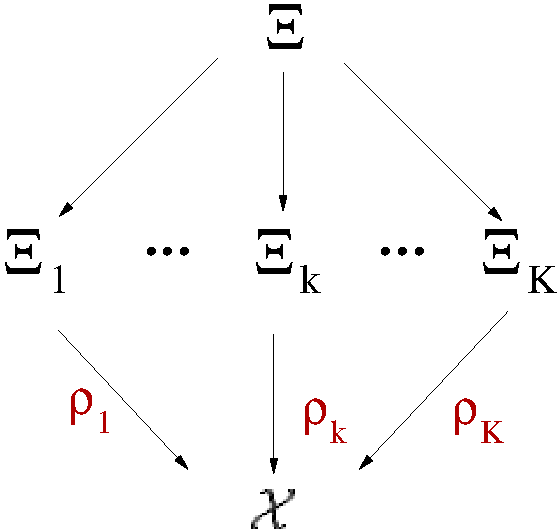
\includegraphics[scale=0.35]{gen-model-orig-proj.pdf}
\caption{Multiple Sensor setting}
\label{fig:fig1}
\end{figure}


We assume some objects lie in some "object`` space $\Xi$, and each sensor has another "view`` of the objects. The measurements recorded by the $i^{th}$ sensor lie in some "measurement space`` $\Xi_i$. The usual approach in pattern recognition is to use feature extractors on the spaces to get a feature representation in Euclidean space and use classical pattern recognition tools to carry out the exploitation task. The alternative approach is to acquire dissimilarities between the group of objects, and use the dissimilarities to either find an embedding in a low-dimensional Euclidean space where classic statistical tools are available for inference or use dissimilarity-based versions of pattern recognition tools~\cite{duin2005dissimilarity}. We will follow the embedding approach in a  low-dimensional Euclidean space where small number of dimensions allow us to avoid "curse of dimensionality``. We will require the embeddings of dissimilarities from  different conditions to be "commensurate`` so that sensor measurements can be compared or jointly used in inference. This is accomplished by maps $\rho_k,k=1,\ldots,K$ from measurement spaces $\Xi_k$ to a low-dimensional commensurate space $\mathcal{X}$ visualized in~\ref{fig:fig1}. Learning these maps from data is  an important portion of our approach.

There are quite  a few real life cases, where the data is acquired or available exclusively in dissimilarity representation instead of feature representation~\cite{CMDS,borg+groenen:1997,duin2005dissimilarity}.
 Multidimensional scaling is the processing step used to find the feature representation equivalent of this kind of data, so that  statistial machine learning methods can be applied to the data. A specific variant of MDS will be used to get an embedding in  Euclidean Space. Multidimensional scaling computes a configuration of points that has interpoint distances as close as possible to the dissimilarities in dissimilarity representation. Different criterion functions can be used to measure how close the distances are  to the given dissimilarities, the optimization of which leads to different embedded configurations. Among these, we seek configurations that have  the merit of  as close as possible to (in some sense) optimal in terms of the exploitation task we are interested in. In this paper, hypothesis testing is our exploitation task, and  by "optimal'' we mean the one that leads to the  test with  the highest power. Consider the weighted raw-stress function:
\begin{equation}
\sigma_{W}(X)=\sum_{1\leq s\leq n;1\leq t\leq n} {w_{st}(d_{st}(X)-\delta_{st})^2  }\label{raw-stress}
\end{equation}
 for an  $n \times p$ configuration matrix ($n$ points in $p$ dimensions)  $X$  where $d_{st}(X)$ is the Euclidean distance between $s^{th}$ and $t^{th}$ rows of $X$ and $w_{st}$ is the weight for $st^{th}$  squared difference.  We will refer to the $n \times n$  matrix representation of the weights and Euclidean distance as $W$ and $D(X)$, respectively. This   criterion function which will be minimized for embedding configurations is appropriate for our purpose of finding a tradeoff between two different criteria (namely the preservation of fidelity and commensurability).




Let us state the dissimilarity-representation version of a hypothesis testing problem:\\
$n$ different objects/instances are measured/judged under $K$ different conditions with (possibly notional) measurements $x_{ik}$ indexed by object and condition. Each of the measurements $x_{ik}$ lies in  the corresponding space $\Xi_k$. 
\[  \begin{array}{cccc}
        & \Xi_1 & \cdots & \Xi_K\\
        Object ~ 1 & \bm{x}_{11} & \sim \cdots \sim & \bm{x}_{1K} \\
        \vdots & \vdots & \vdots & \vdots \\
        %\text{Object} ~ i & \bm{x}_{i1} & \sim \cdots \sim & \bm{x}_{iK} \\
        %\vdots & \vdots & \vdots & \vdots \\
        Object ~ n & \bm{x}_{n1} & \sim \cdots \sim & \bm{x}_{nK}
      \end{array}      
\]
To each pair of measurements $x_{ik},x_{jk}$ in the same space, we can assign a dissimilarity value $\delta_{ijk}=\delta\{x_{ik},x_{jk}\}$, possibly dependent on the space $\Xi_k$. We assume the dissimilarities to be non-negative and  symmetric, and 0 for $\delta\{x_{ik},x_{ik}\}$  It is these  dissimilarities we utilize to do inference on the following exploitation task:

 Given dissimilarities between  $K$ new measurements/observations($\bm{y}_{k};;k=1,\ldots,K$) and the previous 
$n$ objects under $K$ conditions, we wish to test  $K$ measurements $\bm{y}_1,\ldots,\bm{y}_k,\ldots,\bm{y}_K ,\hspace{3pt} \bm{y}_k\in\Xi_k$,  that ``these measurements are from the same  object"  versus the alternative hypothesis that ``they are not  from the same  object"~\cite{JOFC}:
    \[
\begin{array}{l}
%\hspace{-2em}
    H_0: \bm{y}_{1} \sim \bm{y}_{2} \sim \cdots \sim \bm{y}_{K}
 \text{ versus } 
 H_A: \exists i, j , 1\leq i < j \leq K :\bm{y}_{i} \nsim \bm{y}_{j}  
\end{array}
\]
We can restate the null hypothesis as the case where the dissimilarities are ``matched" and the alternative as the case where they are not ``matched".

Dissimilarities are in the form  of $n \times n$  dissimilarity matrices $\{\Delta_k;k=1,\ldots,K\}$ with entries $\{\delta_{ijk} ;  i=1,\ldots,n;\hspace{5pt} j=1,\ldots,n\}$  and a  vector (of length $nK$) of dissimilarities  $\mathbf{\Delta}^{new}=\{ \delta_{ik}^{new}; i=1,\ldots, n;\hspace{5pt} k=1,\ldots,K\}  $  where $\delta_{ik}^{new} $ is the dissimilarity  between  $x_{ik}$ and $y_k$

 Since dissimilarities are  measured between pairs of objects under the same condition,
 we have separate dissimilarity matrices , each consisting of dissimilarities between pairs of  measurements for a separate condition.
 Due to the fact that data sources are ``disparate", it is not immediately obvious how  a dissimilarity between an object in one condition and another object in another condition  can be computed, or even defined.  In general, these between-condition between-object  similarities are not available. 

We will assume the number of conditions,K=2 for the  simplicity of presentation. However, our approach is trivially generalizable  to K>2 and we will present our results for a setting where K=3.

\section{``Matched" and ``Conditions" in data}

What we mean by ``conditions" and ``matched" is dependent on the context of the  problem. Conditions could be different modalities of data, e.g., one condition could be  an image of an object, while the other condition could be a text description of the object. ``Matched", in general, means observations of the same object, or realizations of a common concept. Some specific examples include:

  \begin{itemize}
    \item
If the objects are wiki documents, a condition could be the textual content of the wiki document and another condition could be the wiki hyperlink graph. ``Matched'' could mean two  wiki articles ``are on the same topic''.
\item
The condition of a text document can be the language it is in and ``matched'' could mean two documents ``are about the same topic'' or translations of each other.

    \item For photos, ``conditions" are different acquisition conditions and ``matched'' photos mean they are  ``of the same person''. Acquisition conditions could be\\
    \hspace*{0.1 in}-- indoor lighting vs outdoor lighting\\
    \hspace*{0.1 in}-- two cameras of different quality\\
    \hspace*{0.1 in}-- passport photos and airport surveillance photos.
    \item We might be talking about objects in a single space with multiple dissimilarities, where dissimilarities are measured for different purposes, or judged by different people.
  \end{itemize}

\section{Two  models for generating data}
Here we propose two data models that illustrate our idea of matchedness.
\subsection{Gaussian setting\label{subsec:GaussianSet}}
	Let    $\Xi_1 = \mathbb{R}^{p}$ and $\Xi_2 = \mathbb{R}^{p}$.
  Let $\bm{\alpha}_i \sim^{iid} MVNormal(\bm{0},I_p)$ represent $n$ ``objects".  Let $X_{ik} \sim^{iid} MVNormal(\bm{\alpha_i},\Sigma)$ represent $K=2$ matched measurements (each under a different condition).
  $\Sigma$ is a positive-definite $p\times p$ matrix such that  $\max(\Lambda(\Sigma))=\frac{1}{r} $ where $\Sigma=U\Lambda(\Sigma)U'$  is the eigenvalue decomposition of $\Sigma$. See Figure~\ref{fig:Fig1}.

The parameter $r$ controls the variability between ``matched" measurements. If $r$ is large, we expect the distance between matched measurements
$X_{i1}$ and $X_{i2}$ to be stochastically smaller than $X_{i1}$ and $X_{i'2}$ for $i \neq i'$ ; if r is small, then ``matched" is not informative in terms of similarity of measurements.
 Smaller $r$ will make the decision problem harder and will lead to higher rate of errors or tests with smaller power for fixed type I error rate $\alpha$.
  
    \begin{figure}
	\begin{center}
    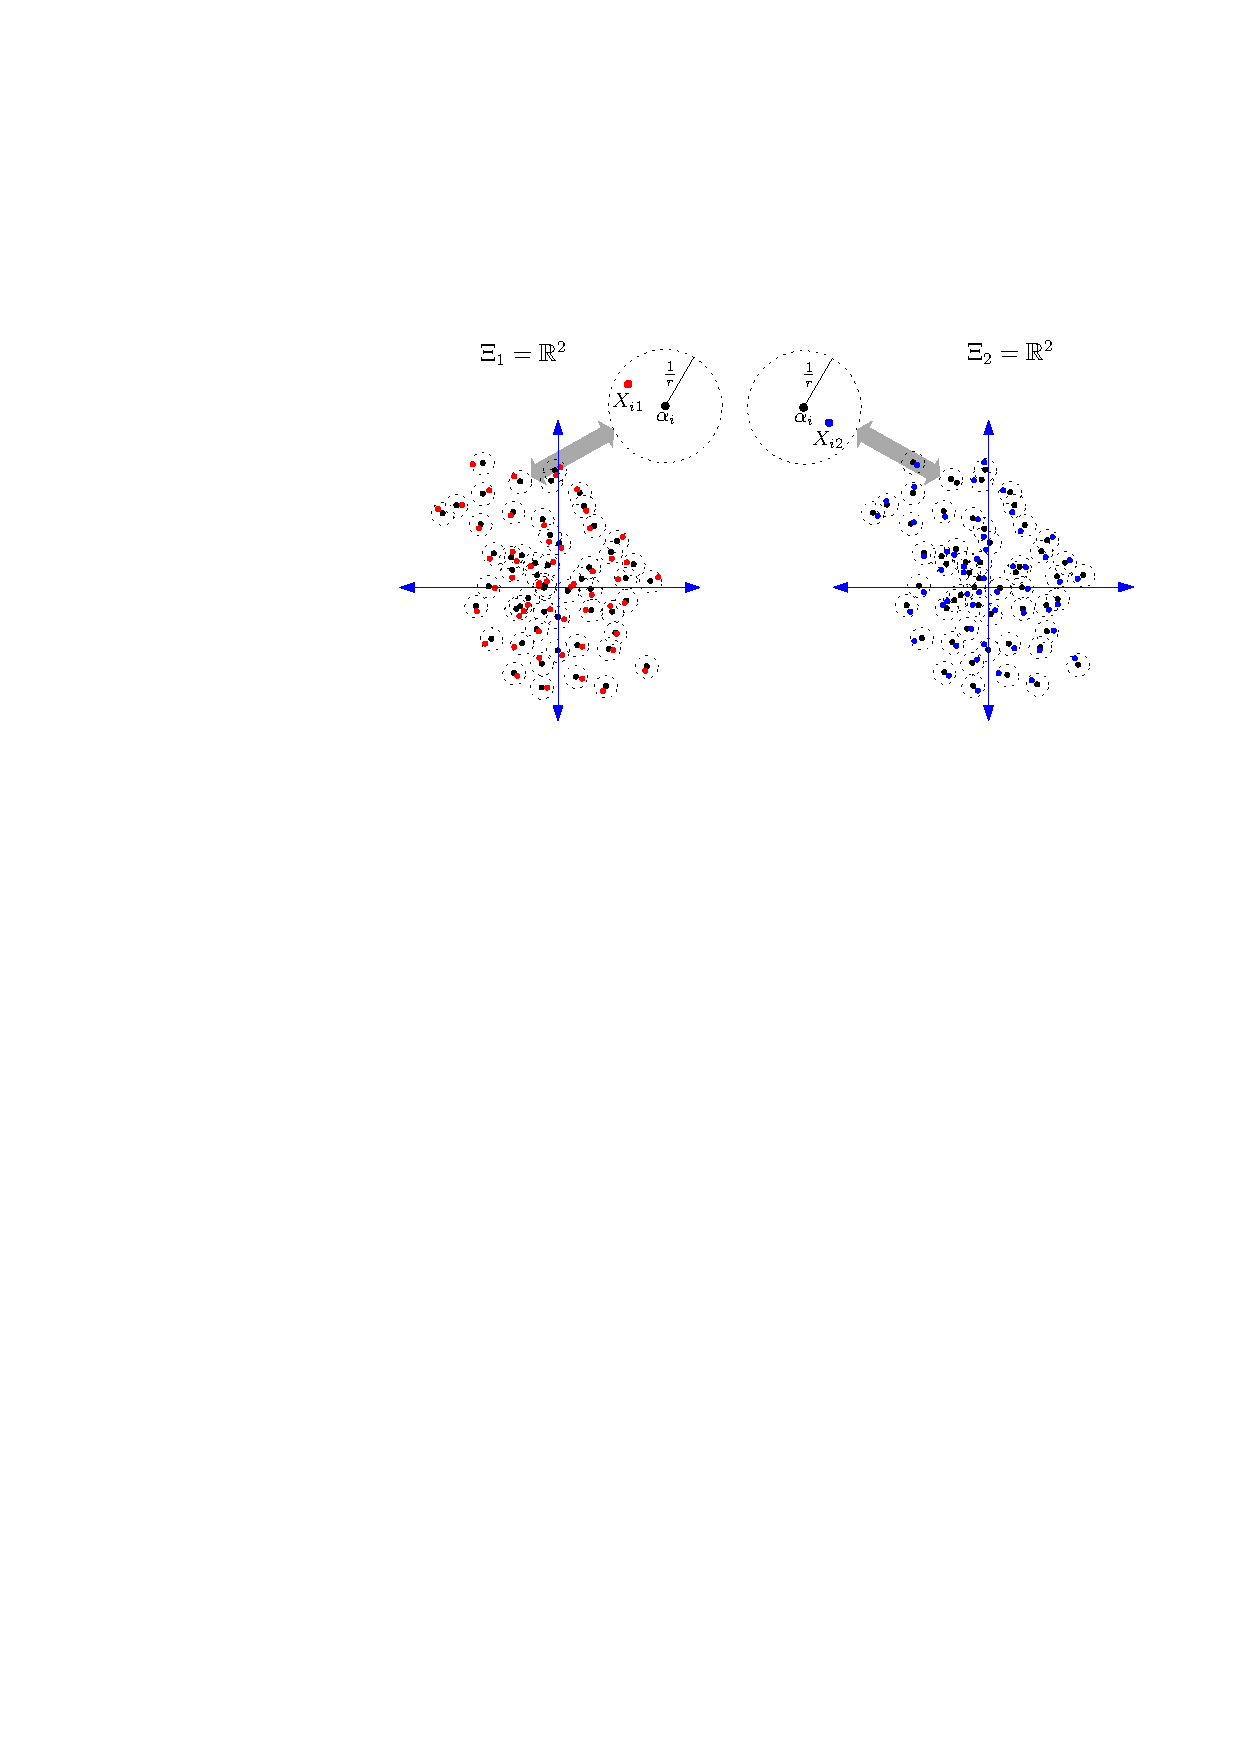
\includegraphics[scale=0.75]{MVN_alpha_r_multiple_sancar.pdf}
    \caption{For the  Gaussian setting (Section \ref{subsec:GaussianSet}), the $\alpha_i$ are denoted by black points and the $X_{ik}$ are denoted by red and blue points respectively.}
\label{fig:Fig1}
	\end{center}
  \end{figure}

\subsection{Dirichlet setting\label{subsec:DirichletSet}}
Let $S^p=\{\bm{x}:\bm{x}\in\mathbb{R}^{(p+1)}, \sum_{l=1}^p{x_l}=1\}$ be the standard $p$-simplex in $\mathbb{R}^{p+1}$.
 Let $\Xi_1 = S^p$ and $\Xi_2 = S^p$.   Denote a vector of ones by $\bm{1}_{p+1}\in \mathbb{R}^{(p+1)}$.
  Let $\bm{\alpha}_i \sim^{iid} Dirichlet(\bm{1}_{p+1})$ represent $n$  ``objects'' and let $X_{ik} \sim^{iid} Dirichlet(r\bm{\alpha}_i+\bm{1}_{p+1})$ represent $K$ measurements. See Figure~\ref{fig:Fig2}.

 The parameter $r$ again controls the variability between ``matched" measurements.
    \begin{figure}
	\begin{center}
    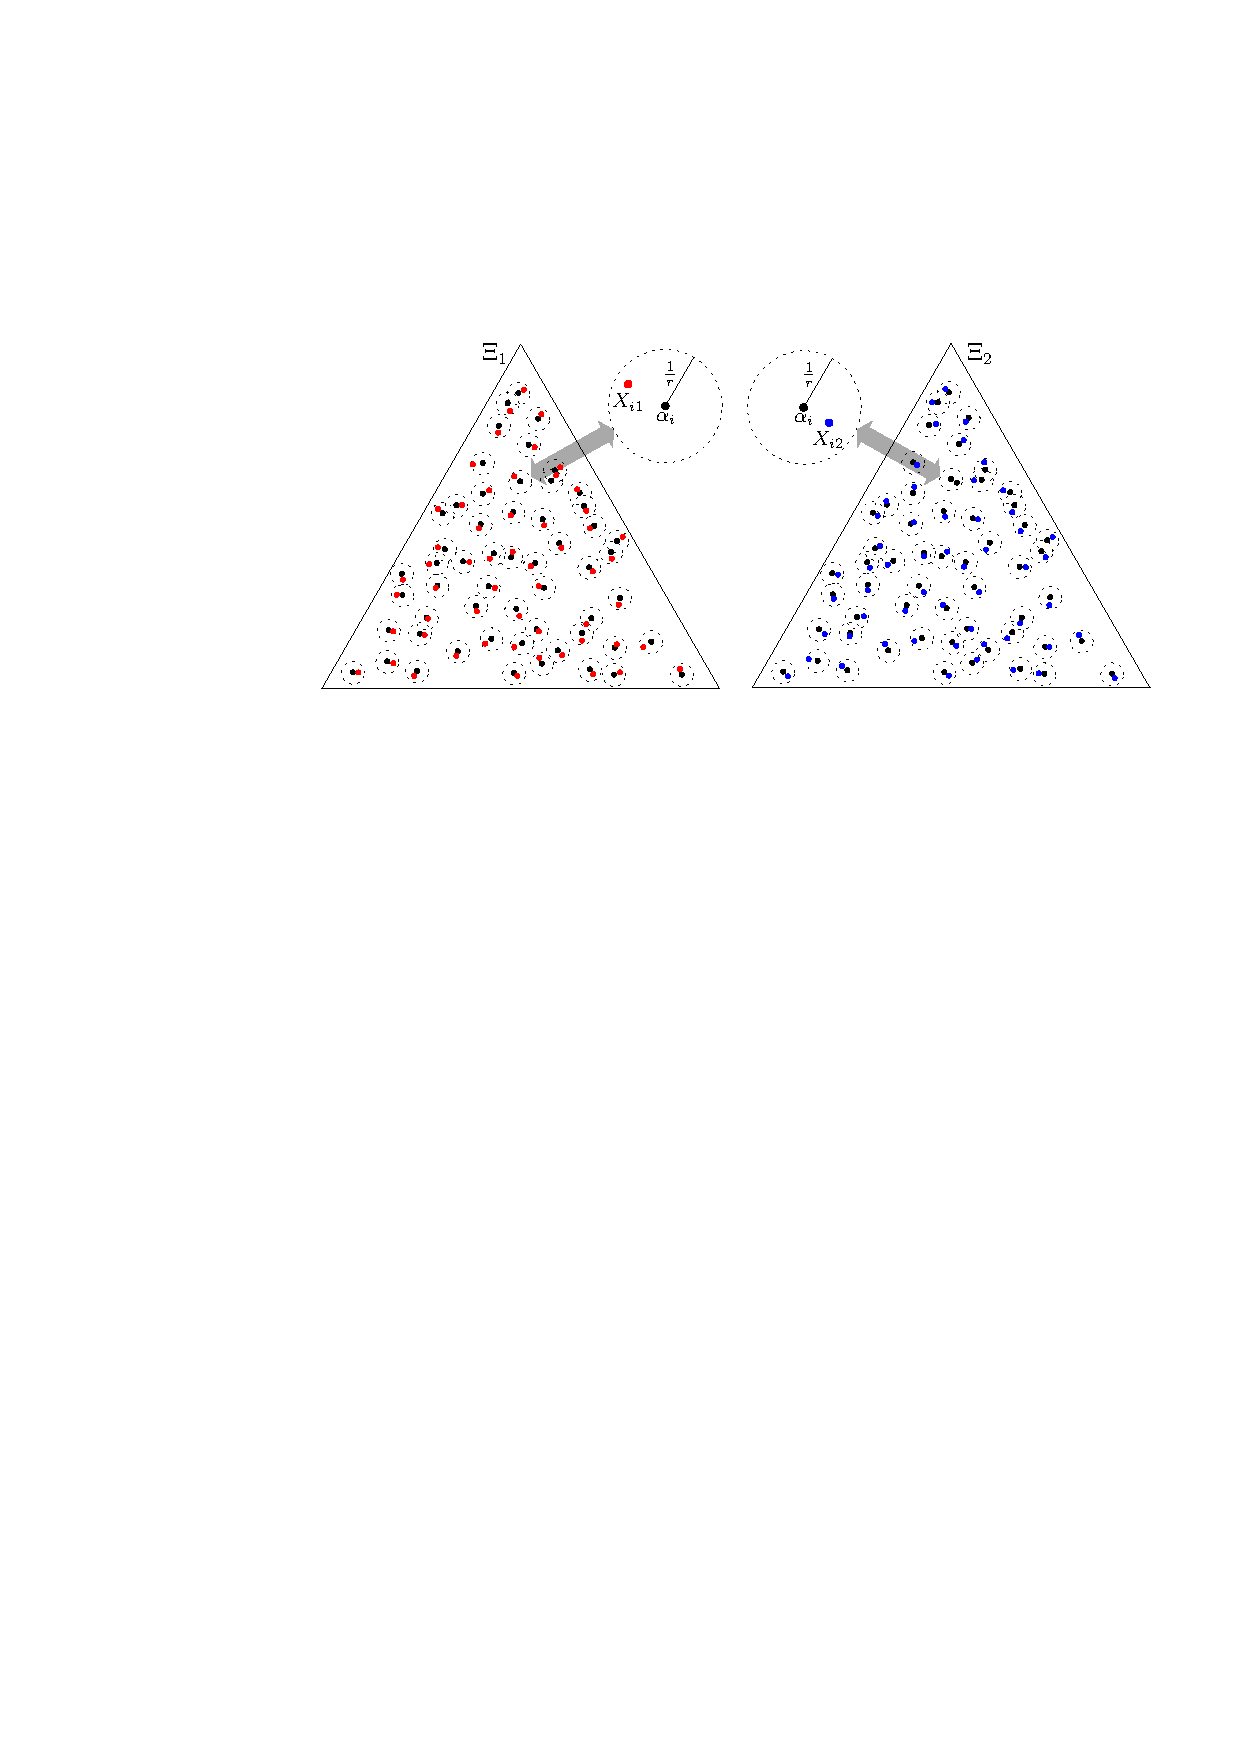
\includegraphics[scale=0.75]{Dirichlet_alpha_r_multiple_sancar.pdf}
   \caption{ For the  Dirichlet setting (Section \ref{subsec:DirichletSet}),  the $\alpha_i$ are denoted by black points and the $X_{ik}$ are denoted by red and blue points respectively.}
\label{fig:Fig2}
	\end{center}
  \end{figure}

\subsection{Noise\label{noise}}
Measurements $X_{ik}$ carry the signal that is relevant to our exploitation task. Noise dimensions can be introduced to  the measurements by concatenating a $q$-dimensional error vector whose magnitude is controlled by the parameter $c$. The noisy measurements will be  represented by the random vectors 
 \begin{equation}
\breve{X}_{ik}=[(1-c)X_{ik}\hspace{5pt} cE_{ik}]\label{eq:noise-expr}
\end{equation}
 where $E_{ik} \sim^{iid} Dirichlet(\bm{1}_{(q+1)})\label{eq:noise-model-dir} $ for the Dirichlet setting and $E_{ik} \sim^{iid} MVNormal(\bm{0} , (1+\frac{1}{r})I_{q+1}) \label{eq:noise-model-mvn} $ for the Gaussian setting. $\breve{X}_{ik}$ will be used instead of ${X}_{ik}$ for computing dissimilarities in the ``noisy" version of the problem. These noisy measurements allow the comparison of  different methods applied to the problem with respect to their robustness.
  

\section{Manifold Matching\label{sec:JOFC}}
  Our approach can be summarized as  ``manifold matching", which is defined as simultaneous ``manifold learning" and ``manifold alignment" -- identifying embeddings of multiple disparate data sources into the same low-dimensional space where joint inference can be pursued. The inference task either requires the fusion of data from disparate sources( as in the test of matchedness) or gathers performance gains from the fusion. The assumption is that the data in each measurement space lie approximately in a low dimensional manifold. An effort is made to match the low-dimensional manifolds so that matched measurements from different conditions are as close as possible to each other.  The embeddings from the dissimilarities in the measurement spaces into the commensurate space are implicit mapping from the measurement space($\Xi_k$)  to the commensurate space( $\mathcal{X}$ in ~\ref{fig:fig1}). The learning problem involves estimating these maps(whether implicit as in the dissimilarity representation of multiple sensor measurements or explicit in the  feature representation setting)  from a training data of matched measurements.


We will assume  the commensurate space  $\mathcal{X}$  is  $\mathbb{R}^d$ where $d$ is pre-specified. The selection of $d$ -- model selection -- is  a task that requires much attention and is  beyond the scope of this article.






To embed dissimilarities  $\{\Delta_k,k=1 ,\ldots,K\}$  from different conditions into a commensurate space in one step, an omnibus dissimilarity matrix  $M$ can be embedded in the low-dimensional Euclidean spaceinto one omnibus dissimilarity matrix $M$, imputing entries if necessary. Consider, for $K=2$, \begin{equation}
M=  \left[ \begin{array}{cc}
         \Delta_1 & L\\
        L^T  & \Delta_2 
     \end{array}  \right]     \label{omnibus} 
\end{equation} where $L$ is a matrix of imputed entries. One way to impute $L$ is to set it to $\frac{\Delta_1+\Delta_2}{2}$. Another choice for imputation is introduced in \ref{sec:FidComm}: the diagonal of $L$ is set to 0, the rest of the entries are $NA$ and are ignored in the optimization of MDS criterion.  
Using MDS to embed  this omnibus matrix into a  space  $\mathcal{X}$, we obtain $2n$ embedded observations $\{\tilde{y}_i^{(k)}; i=1,\ldots,n;k=1,2\}$ in a single space, with distances between the different observations consistent with the given dissimilarities. Now that the observations are commensurate, we can compute the test statistic \[
\tau=d\left(\tilde{y}_i^{(1)},\tilde{y}_j^{(2)}\right)\label{teststat}
\] for $i^{th}$ and $j^{th}$ observations under different conditions.  For ``large" values of $\tau$, we will reject the null hypothesis. We will refer to this approach as the Joint Optimization of Fidelity and Commensurability (JOFC) approach, for reasons that will be explained in Section \ref{sec:FidComm}. In this approach, the mappings   $\{ \rho_k,; k=1,\ldots,K\}$ in ~\ref{fig:fig1}  are not explicitly defined.


In any exploitation task that necessitates such an matching of manifolds or where the matching is expected to  improve performance, the omnibus embedding approach can be used  to embed the observations in a single space where they are commensurate. 


\subsection{Out-of-sample Extension}
Manifold learning algorithms computes embeddings of training data on low-dimensional manifolds, however they may not always give a map as output  to  be used to compute embeddings of new points. Applying manifold learning algorithms to the combination  of training and test data  will give us such a map, but this would need to be repeated for any new test point, and embeddings of training dissimilarities would be  partially dependent on test data. The solution is to extend the embeddings of training dissimilarities by out-of-sample embedding the test dissimilarities. 
In our hypothesis testing task, we are given dissimilarities   between a new pair of test observations and the previous $nK$ training observations. As embedding the original (in-sample) $nK \times nK$ dissimilarities between training observations doesn't result in a explicit map, we require out-of-sample embedding.  Out-of-sample extension for MDS will be used throughout this paper\cite{TrossetOOS}. 

% - given the embedded configuration $X$ of the 
%training observations and the augmented dissimilarity matrix that includes dissimilarities between test observations and %the training observations, and dissimilarities in between the training observations, oos-embedding consists of embedding
%the test points into  the existing configuration so as to be as consistent as possible with these dissimilarities (the distances %between points are as close as possible to the dissimilarities as measured by the criterion function). 
Out-of-sample embedding can be done one observation at a time, or jointly if the dissimilarities among multiple test observations are also available. 


\section{Fidelity and Commensurability constraints for Manifold Matching\label{sec:FidComm}}
Unless 
\begin{itemize}
\item the dissimilarity matrix is the Euclidean distance matrix of the original observations, and, 
\item the embedding dimension is greater or equal to the dimension of the original observations,
\end{itemize}
MDS with raw stress will not result in a perfect reconstruction  of the original observations. Note that we are not neccessarily interested in perfect reconstruction, but the best embedding for our exploitation task which is to test whether two sets of dissimilarities are ``matched". The following two criteria  are guidelines for what the manifold matching should accomplish andhelpful for optimizing the matching for the exploitation task we are to carry out.


\begin{itemize}
\item Fidelity is how well the mapping to commensurate space preserves the original dissimilarities.
Our within-condition {\em fidelity error} is given by
    \[
\epsilon_{f_{k}} = \frac{1}{{{n}\choose{2}}} \sum_{1 \leq i < j \leq n} (d(\widetilde{\bm{x}}_{ik},\widetilde{\bm{x}}_{jk})-\delta_k(\bm{x}_{ik},\bm{x}_{jk}))^2
\] 
where ${\bm{x}}_{ik}$ is the original observation of the $i^{th}$ object for the $k^{th}$  condition and $\widetilde{\bm{x}}_{ik}$ is the embedded configuration of the $i^{th}$ object  for the $k^{th}$ condition;  $d(\cdot,\cdot)$ is the Euclidean distance function (for the embedding space) and $\delta_k(\cdot,\cdot)$ is the dissimilarity function defined for objects in the $k^{th}$ condition.

\item Commensurability is how well the mapping to commensurate space preserves matchedness of matched observations. Between-condition {\em commensurability error} is given by
    \[
\epsilon_{c_{k_1k_2}} = \frac{1}{n} \sum_{1 \leq i \leq n;k_1 <k_2} (d(\widetilde{\bm{x}}_{ik_1},\widetilde{\bm{x}}_{ik_2})-{ \delta_{k_1k_2}}(\bm{x}_{ik_1},\bm{x}_{ik_2}))^2
\label{comm-error}
\]
 for conditions $k_1$ and $k_2$; $\delta_{{k_1}{k_2}}(\cdot,\cdot)$ is the (notional) dissimilarity function between measurements in  $k_1^{th}$ and $k_2^{th}$ conditions. Note that ,in general, there are $K$  within-condition fidelity error terms and $\frac{K \times (K-1)}{2}$  between-condition commensurability error terms.

Although  the between-condition dissimilarities of the same object, ${ \delta_{k_1k_2}(\bm{x}_{ik_1},\bm{x}_{ik_2}})$, are not available,  it is not unreasonable in this setting  to set ${ \delta_{k_1k_2}}(\bm{x}_{ik_1},\bm{x}_{ik_2}) = 0$ for all $i,k_1,k_2$.  So we choose diagonal  entries of $L$ in  equation \eqref{omnibus} to be all zeroes. Setting these diagonal entries to zero forces matched points to be embedded close to each other. We ignore the possibility that this choice for between-condition dissimilarities might not be optimal, in order to concentrate on the main problem.

Then, the commensurability error  term becomes
  \[
\epsilon_{c_{k_1k_2}} = \frac{1}{n} \sum_{1 \leq i \leq n;k_1< k_2} (d(\widetilde{\bm{x}}_{ik_1},\widetilde{\bm{x}}_{ik_2})))^2
\]
\end{itemize}

 There is also between-condition {\em separability error} given by
    $$\epsilon_{s_{k_1k_2}} = \frac{1}{{{n}\choose{2}}} \sum_{1 \leq i < j \leq n;k_1 <k_2} (d(\widetilde{\bm{x}}_{ik_1},\widetilde{\bm{x}}_{jk_2})-{ \delta_{k_1k_2}}(\bm{x}_{ik_1},\bm{x}_{jk_2}))^2.$$ This error will be ignored herein, due to the fact that 
$\delta_{k_1k_2}(\bm{x}_{ik_1},\bm{x}_{jk_2})$ is not  available. Although it is possible to impute these dissimilarities, the optimal  imputation is an open question and ignoring these terms provides for investigation of simpler, still open questions.


Note that the omnibus embedding approach tries to jointly optimize fidelity and commensurability , by minimization of some measure of discrepancy between the given dissimilarities (all of which are between-condition or within-condition dissimilarities) and the distances of the embedded configuration. This is most obvious in the  raw stress version of  MDS, since the individual terms can be separated according to whether they are contributing to  fidelity or  commensurability  error.

 Consider the weighted raw stress criterion $\sigma_{W}(\cdot)$ with a weighting matrix $W$, given in equation~\eqref{raw-stress}.
 The omnibus matrix $M$ we are considering is a partitioned matrix consisting of matrices from different conditions ($k={1,2}$), so we index the entries of the matrix  by 4-tuple ${i,j,k_1,k_2}$ which refers to the entry in the $i^{th}$ row and $j^{th}$ column of the submatrix in  the $k_1^{th}$  row partition and   $k_2^{th}$ column partition. For example, the entry ${M}_{2n,n}$ will have the indices $\{i,j,k_1,k_2\}=\{n,n,2,1\}$ in the new indexing scheme. $D(\cdot)$ and $W$, which are the same size as $M$, follow the same 4-tuple indexing. Then,
 
\begin{align}
\sigma_W(\cdot)  &= & &\sum_{i,j,k_1,k_2} {w_{ij{k_1}{k_2}}(d_{ij{k_1}{k_2}}(\cdot)-M_{ijk_1k_2})^2 } \notag\\
\hspace{3pt} &=& &\underbrace{\sum_{i=j,k_1<k_2}  {w_{ij{k_1}{k_2}}(d_{ij{k_1}{k_2}}(\cdot)-M_{ijk_1k_2})^2}}_{Commensurability}  \hspace{10pt}  &  + &\hspace{2.5em} \underbrace{\sum_{i<j,k_1=k_2}  {w_{ij{k_1}{k_2}}(d_{ij{k_1}{k_2}}(\cdot)-M_{ijk_1k_2})^2  }  } _{Fidelity}\notag\\
\hspace{3pt}&+&  &\underbrace{\sum_{i< j,k_1<k_2}  {w_{ij{k_1}{k_2}}(d_{ij{k_1}{k_2}}(\cdot)-M_{ijk_1k_2})^2  }  } _{Separability}\label{eq:FidCommSep}\hspace{10pt} .
\end{align}


\begin{comment}
\begin{eqnarray}{ccc}
\sigma_W(\cdot)\hspace{3pt}   &= &\sum_{i,j,k_1,k_2} {w_{ij{k_1}{k_2}}(d_{ij{k_1}{k_2}}(\cdot)-M_{ijk_1k_2})^2 } \notag\\
\hspace{3pt} &= &\underbrace{\sum_{i=j,k_1\neq k_2}  {w_{ij{k_1}{k_2}}(d_{ij{k_1}{k_2}}(\cdot)-M_{ijk_1k_2})^2}}_{Commensurability}  \hspace{10pt}  &  + & \underbrace{\sum_{i\neq j,k_1=k_2}  {w_{ij{k_1}{k_2}}(d_{ij{k_1}{k_2}}(\cdot)-M_{ijk_1k_2})^2  }  } _{Fidelity}\notag\\
\hspace{3pt}&+ &\underbrace{\sum_{i\neq j,k_1\neq k_2}  {w_{ij{k_1}{k_2}}(d_{ij{k_1}{k_2}}(\cdot)-M_{ijk_1k_2})^2  }  } _{Separability}\label{eq:FidCommSep2}\hspace{10pt} .
\end{eqnarray}
\end{comment}


Since we set ${ \delta_{k_1k_2}}(\bm{x}_{ik_1},\bm{x}_{ik_2}) = 0$, the corresponding entries of $M$ in the commensurability terms will be 0.

Since we choose to ignore  the separability error, we choose the weights for separability terms to be 0. This also means off-diagonal elements of $L$ in equation \eqref{omnibus} can be ignored. When separability terms are removed from equation \eqref{eq:FidCommSep}, the resulting equation  is a sum of fidelity and commensurability error terms:


\begin{align}
\sigma_W(\cdot)\hspace{3pt}   
\hspace{3pt}&=&\underbrace{\sum_{i=j,k_1< k_2}  {w_{ij{k_1}{k_2}}(d_{ij{k_1}{k_2}}(\cdot))^2}}_{Commensurability}  \hspace{10pt}  &  +&\underbrace{\sum_{i< j,k_1=k_2}  {w_{ij{k_1}{k_2}}(d_{ij{k_1}{k_2}}(\cdot)-M_{ijk_1k_2})^2  }  } _{Fidelity}\notag\label{eq:FidCommSep}\hspace{10pt} .
\end{align}

This motivates  referring to our omnibus embedding approach as Joint Optimization of Fidelity and Commensurabilty (JOFC).

Note that for purpose of minimization, setting all weights  ${w_{ij{k_1}{k_2}}}$ equal is equivalent to the unweighted raw stress $\sigma(X)$:
\begin{equation}
\sigma(X)=\sum_{1\leq s\leq n;1\leq t\leq n} {(d_{st}(X)-\delta_{st})^2  }\label{stress}
\end{equation}

\begin{comment}
\subsection{The incommensurability phenomenon from the viewpoint of Fidelity-Commensurability Tradeoff}

\cite{JOFC}  presented a simple example of incommensurability phenomenon, where linear projections resulted in incommensurate linear subspaces with significant probability. Due to symmetry, all projections have the the same fidelity, but there is only one pair of configurations that has  maximum commensurability. So any method that considers both fidelity and commensurability should have equal performance. This would lead one to conclude all $w$ values should be in the set of  $w^*$. 
\end{comment}

\section{Alternative Methodologies}
For the optimization of commensurability with fidelity as  secondary priority, an alternative method is Canonical Correlational Analysis (CCA)~\cite{Hardoon2004}, which aims to find linear subspaces of the Euclidean space  such that the projection of data points to those subspaces results in  vectors that are maximally correlated. CCA finds a basis for these subspaces iteratively: For each new component in the basis, CCA finds the pair of directions that maximizes correlation with the constraint that the projections along the new directions are  uncorrelated  with projections along previous components. The latter constraint results in  additional preservation of fidelity for each new direction. For the optimization of fidelity,  one can use Principal Components Analysis (PCA), which aims to find linear subspaces such that  projection of data points to those subspaces results in observation vectors that represent the original data as best as possible. To optimize commensurability as  secondary priority, one can use the projections computed by PCA to  compute a Procrustes transformation that will make the projections commensurate. Since the data is originally in a dissimilarity representation, we can directly embed in the low-dimensional space and use Procrustes Analysis to find a mapping between the two separate embeddings. The equivalence of PCA and Classical Multidimensional Scaling~\cite{CMDS} under certain conditions suggests that this approach is the right analog of Procrustes $\circ$ PCA to utilize when in a dissimilarity setting. 

 The omnibus embedding  approach is expected to be more powerful for the exploitation task than either of  the sequential optimizations, since the exploitation task (testing matchedness) requires both optimization of fidelity and commensurability.

\subsection{Procrustes Analysis on Multidimensional Scaling Embeddings\label{subsec:PoM}} 
Since separate  condition dissimilarities are available, a straightforward approach is to embed each conditional dissimilarity matrix, $\Delta_1$ and $\Delta_2$, separately  in  $d$-dimensional Euclidean space (call these embedded configurations $X_1$ and $X_2$, respectively) and then find a mapping function $\rho :\mathbb{R}^{d}\rightarrow\mathbb{R}^{d}$ that maps each point in $X_2$ to approximately its corresponding point in $X_1$. This approach can be seen as a specific example of the general setting where the commensurate space is d-dimensional  Euclidean space and $\rho_1$ in  ~\ref{fig:fig1} is the identity map. 

Estimation of $\rho$ is carried out using  Procrustes Analysis  on training data. Procrustes Analysis~\cite{Sibson} finds a orthonormal matrix $\mathbf{Q}^*$ that minimizes the sum of squared distances between the  target configuration $X_1$ and  the configuration $X_2$ transformed by $\mathbf{Q}^*$, i.e.,
 \[\mathbf{Q}^* = \argmin_{Q^TQ = I} \|X_1 - X_2Q\|_F\] 
 where $\|\cdot\|_F$ is the Frobenius norm on matrices. The map $\rho$ estimated by the linear map $\mathbf{Q}^*$   makes the separate MDS embeddings as commensurate as possible. Once such a mapping is computed, one can out-of-sample embed  new dissimilarities for each condition (separately)  and  use $\mathbf{Q}^*$ to make the embeddings commensurate.
One can then compute the test statistic $\tau$ (the distance between commensurate embeddings) for  the hypothesis testing problem. We will refer to this approach as P$\circ$M - Procrustes $\circ$MDS.

Note that the Procrustes transformation $\mathbf{Q}^*$  is limited to  a linear transformation consisting of rotation and reflection and possibly also scaling components. The optimal mapping might  very well be   non-linear. If we allow  a larger class of mappings to be considered, we would have a smaller model bias for the mapping function, but we would be paying for it  in the form of larger variability. By only considering the class of linear transformations, we are able  to learn $\mathbf{Q}^{*}$ with our limited dataset.


\subsection{Canonical Correlational  Analysis on Multidimensional Scaling Embeddings} 

Again MDS is used  to compute embedding configurations, $ X_1$ and $X_2$. We want to embed into the highest dimensional space  possible ($\mathbb{R}^{d'}$ where $d'=p+q$ for our Gaussian and Dirichlet settings)  to  preserve as many of the signal dimensions as possible (at the risk of possibly including  some noise dimensions). CCA~\cite{Hardoon2004}, then,  yields two mappings $\mathcal{U}_1$ and $\mathcal{U}_2$ that map these embeddings in $\mathbb{R}^{d'}$ to  the low-dimensional commensurate space ($\mathbb{R}^d$). 

\subsubsection*{Canonical Correlational Analysis}

 Let $X$ and $Y$ be two $s$-dimensional random vectors. If  one wants to find  the pair of linear projection operators $U_1:\mathbb{R}^s \rightarrow  \mathbb{R}$, $U_2 :\mathbb{R}^s \rightarrow  \mathbb{R}$ that maximize correlation between the projections of   $X$ and $Y$, CCA finds the solution as stated in the  optimization problem
$$
{\hat{u}_1 ,\hat{u}_2}=\arg\max_{u_1\in\mathbb{R}^s,u_2\in\mathbb{R}^s} {\frac{E[u_1^{T}XY^Tu_2]}{{E[u_1^{T}XX^T u_1]}{E[u_2^{T}YY^T u_2]}}}$$
with the constraints $E[{u_1^{T}XX^T u_1}]=1 , E[{u_2^{T}YY^T u_2}]=1$ for uniqueness. The constraints simplify the optimization function to $$
\arg\max_{u_1\in \mathbb{R}^s,u_2\in \mathbb{R}^s} {E[u_1^{T}XY^Tu_2]}.$$

If the projections are to a pair of $d$-dimensional linear subspaces, the additional pairs of projection vectors can be computed sequentially, with the constraints that the projections along the new directions are uncorrelated with  projections along previous directions. That is, $i^{th}$ pair of directions  that maximize correlation is computed by 
$$
{\hat{u}_{1(i)},\hat{u}_{2(i)}}=\arg\max_{u_{1(i)},u_{2(i)}\in\mathbb{R}^s} {E[u_{1(i)}^{T}XY^Tu_{2(i)}]}.$$ subject to constraints $E[{u_{1(i)}^{T}XX^T u_{1(i)}}]=1$ , $E[{u_{2(i)}^{T}YY^T u_{2(i)}}]=1$, $E[{u_{1(i)}^{T}XX^T u_{1(j)}}]=0$,  
   $ E[{u_{2(i)}^{T}YY^T u_{2(j)}}]=\nolinebreak0$ $\forall \quad  j=1,\ldots,i-1$. For sample CCA, $E[XX^T]$,$E[YY^T]$ and $E[XY^T]$ are replaced with their sample estimates. The direction vectors ${\hat{u}_{1(i)},\hat{u}_{2(i)}}, i=1,\ldots,d $ form the rows of projection matrices which represent the mappings $\mathcal{U}_1$ and $\mathcal{U}_2$. 


Note that $s$, the dimension of $X$ and $Y$, is the embedding dimension $d'$  in the CCA approach. 


As in P$ \circ $M, new dissimilarities are out-of-sample embedded and mapped to a commensurate  space by maps provided by CCA. We can now compute the test statistic  and reject the null hypothesis for ``large'' values of the test statistic $\tau$  as in Section \ref{subsec:PoM}.


\subsection{Relation of $P\circ M$ and Joint Optimization of Fidelity and Commensurability} 

Suppose we let $w_{ijk_1k_2}=w$ for commensurability terms and $w_{ijk_1k_2}=1-w$ for fidelity terms in equation \eqref{eq:FidCommSep}. For the resulting weight matrix $W$, define 
\begin{equation}
f_w(D(\cdot),M) = \sigma_W(\cdot) \label{fid-comm-tradeoff-func}
\end{equation}
 where $M$ is the omnibus matrix obtained from  a given pair of dissimilarity matrices, $\Delta_1$ and $\Delta_2$, as in equation \eqref{omnibus}.   As $w$ goes to 0, the configuration embedded by JOFC converges to a configuration equivalent to (up to rotation and reflection)  the configuration embedded by P$\circ$M.


\begin{thm}
Define $\sigma(\cdot)=\sigma_{W=\bm{1}}(\cdot)$ (unweighted raw stress) where $\bm{1}$ is a matrix of 1's.
 Let $\mathbf{X}_1$ and $\mathbf{X}_2$ be the corresponding $n\times p$ configuration matrices with column means of $\bm{0}$ (obtained from separately embedding  $\Delta_1$ and $\Delta_2$ by minimizing the raw stress $\sigma(\cdot)$ ). 
Let  $\mathbf{Q}=\argmin_{\mathbf{P^T}\mathbf{P}=\mathbf{P}\mathbf{P^T}=\mathbf{I}}||{\mathbf{X}_1-\mathbf{X}_2}\mathbf{P}||^2$ ,   $\mathbf{\tilde{X}}_2= \mathbf{X}_2\mathbf{Q}$, 
and let  
$\mathbf{X}=\left[\begin{array}{c}
\mathbf{X}_1\\
\mathbf{\tilde{X}}_2
\end{array}\right]$.

For $w>0$, let $\mathbf{Y}_{w} = \left[\begin{array}{c}
\mathbf{Y}_1\\
\mathbf{Y}_2
\end{array}\right]$  be  a $2n \times p$ configuration matrix obtained by minimization of 
$ f(\mcY, M) =(1-w)\left({\sigma{(\mcY_1)}}+{\sigma{(\mcY_2)}}\right)+w||{\mcY_1-\mcY_2}||^2 $ with respect to  $\mcY=\left[\begin{array}{c}
\mcY_1\\
\mcY_2
\end{array}\right]$ with the constraint that $\mcY_1$ and $\mcY_2$ are two $n \times p$ configuration matrices having column means of $\bm{0}$. Then, $$lim_{w\rightarrow0}\mathbf{Y}_{w}=\mathbf{X}\mathbf{R}$$ for a $p\times p$ orthonormal matrix $\mathbf{R}$. ($\mathbf{R}$ is a transformation matrix with a rotation and possibly a reflection component.)
\end{thm}
 

\subsection{Relation of CCA and Commensurability} 

\begin{thm}
Let $ \mathcal{U}$ be the set of all orthogonal d-frames 
(ordered set of d linearly independent vectors) of $R^{d'}$. 
Let $X_1$ and $X_2$  be two $n\times d'$ (configuration) matrices that are perfectly ``matched"
 (there exists a transformation matrix $\mathbf{Q}$ such that $\|   X_1\mathbf{Q}  -X_2 \|=0$).
If commensurability is  defined as
in equation~\eqref{comm-error},
 where  the embedded configurations are $\tilde{X_1}=X_1U_1$ and $\tilde{X_2}=X_2U_2$ for some  $U_1\in \mathcal{U}$ and $U_2\in  \mathcal{U}$,
and   the original dissimilarities are $D(X_1)$ and $D(X_2) $,
 CCA on $X_1$ and $X_2$ gives $\mathbf{U}_1\in\mathcal{U}$ and  $\mathbf{U}_2\in\mathcal{U}$, 
 the two elements of $\mathcal{U}$ that maximize commensurability, subject to $U_1^{T}X_1^{T}X_1U_1=I_d$ and $U_2^{T}X_2^{T}X_2U_2=I_d$ ($I_d$ is the $d \times d$ identity matrix).
\end{thm}



\section{Related Work \label{sec:RelatedWork}}
There have many efforts toward solving ``manifold alignment", which is a related  problem. ``Manifold alignment" seeks to find correspondences between observations from different ``conditions". The setting that is most similar to ours is the semi-supervised setting, where a set of correspondences are given and the task is to find correspondences between a new set of points in each condition. In contrast, our hypothesis testing task is to determine whether any given pair of points is ``matched" or not. The proposed solutions follow a common approach in that they look for a common commensurate or a latent space, such that the representations (possibly projections or embeddings) of the observations in the commensurate space match.

Wang and Mahedavan~\cite{Wang2008} suggest an  approach that uses embedding followed by Procrustes Analysis to find a map to a commensurate space. Given a paired set of points, Procrustes Analysis~\cite{Sibson}, finds a transformation from one set of points to another in the same space that minimizes sum of squared distances, subject to some constraints on the transformation. In the case mentioned in \cite{Wang2008}, the paired set of points are corresponding low-dimensional embeddings of kernel matrices.   For the embedding step, they made the choice of using Laplacian Eigenmaps, though their algorithm allows for any appropriate embedding method.

 Zhai et al.~\cite{Zhai2010}  finds two projection matrices to minimize three terms in an energy function similar to our JOFC approach (see Section \ref{sec:JOFC}). One of the terms is the \emph{correspondence preserving term} which is the sum of the squared distances between corresponding points and is analogous to our commensurability error term. The other two terms are \emph{manifold regularization terms} and consist of the reconstruction error for a Locally Linear Embedding of the projected points. These terms, analogous to fidelity, make sure the projections in the lower dimension retain the structure of the original points. For fidelity error terms in our setting, this is done by preserving dissimilarities. For manifold regularization terms, this is done by preserving the local neighborhood of points, such that close points are not mapped apart.
Ham and Lee solve the problem in semi-supervised setting by a similar approach, by minimizing a cost function of three terms, two terms for fidelity of embedding, one term of commensurability.


Another view to look at the data from different sources is to consider disparate data as different views to be reconciled. According to this view, for observations of $n$ objects under $K$ conditions, $n$ points are embedded instead of $nK$ points. Choi et al.\ \cite{Choi:2008:MIM:1619995.1620064} use the Markov random walk interpretation of multiple kernel matrices to combine into one kernel matrix.  Many other ``Multiple Kernel Learning"  methods exist in the literature~\cite{McFee:2011:LMS:1953048.1953063,Lin2009,Lanckriet2004}.

Another approach is Three-way Multidimensional scaling\cite{3wayNMDS,borg+groenen:1997}.
 This approach assumes the  different ``conditions" of the data are linear transformations of a single configuration and aims to find this single configuration. For our setting, one would first embed the in-sample dissimilarities via the three-way MDS, which would give as the linear transformations that map from group configuration to individual configurations under each condition. This is followed by out-of-embedding the OOS dissimilarities, and use the inverse of the transformation matrices to find the out-of-sample embeddings with respect to the group configuration. Since the out-of-sample embeddings are commensurate, the test statistic can be computed as the distance between the OOS embeddings. 

%According to our ideas of tradeoff between fidelity and commensurability, this always maximizes commensurability without regard for fidelity and the constraint of the linear transformations between the group and condition configurations allows the approach to recoup some fidelity. 


\section{Fidelity and Commensurability Tradeoff}
The major question  addressed in this work is whether in the tradeoff between preservation of fidelity and preservation of  commensurability , there is an optimal point for our hypothesis testing task.  The weights in raw stress allow us to answer this question relatively easily. Since in equation \eqref{eq:FidCommSep},  each term indexed with $i$, $j$ is either a fidelity or a commensurability term, setting $w_{ij}$ to $w$ and $1-w$  for commensurability  and fidelity  terms respectively will allow us to control the importance of fidelity and commensurability terms in the optimization by varying $w$. 
\begin{align*}
\sigma_W(X)&=  f_w(D(X),M) & &\\
&=  \underbrace{\sum_{i=j,k_1\neq k_2}  {w(d_{ij{k_1}{k_2}}(X))^2}}_{Commensurability} & +\hspace{2em} & \underbrace{\sum_{i<j,k_1=k_2}  {(1-w)(d_{ij{k_1}{k_2}}(X)-M_{ijk_1k_2})^2  }  } _{Fidelity}\\
&=  \left(w\right)\left(n\right) \epsilon_{c_{k_1=1,k_2=2}} & +\hspace{2em} & (1-w){{n}\choose{2}} ( \epsilon_{f_{k=1}}+\epsilon_{f_{k=2}} )
\end{align*}

Our expectation is that there is a $w^*$ that is optimal for the specific exploitation task (has the best power in hypothesis testing). In fact, our exploratory simulations confirm the power of the tests varies with varying $w$ and indicate the range where the optimal  $w^*$ lies.



\section{Definition of  $w^*$}

Let $\mathbf{F}_m$ be the joint distribution of
$X_m= \left[
 \begin{array}{c}
X_{1m}\\
X_{2m}
\end{array}
\right]$ and 
$\mathbf{F}_u$ be the  joint distribution of
$X_u= \left[
 \begin{array}{c}
 X_{1u}\\
 X_{2u} 
\end{array}
\right]$
 where   $X_{1m},X_{2m}$ are the random vectors of dimension $d'$ for the matched observation pair and $X_{1u},X_{2u}$ are the random vectors of dimension $d'$ for the unmatched data pair.   The constraint on  $\mathbf{F}_m$ is that  correlation  matrix of $X_{1m},X_{2m}$ is non-zero, while  the constraint on $\mathbf{F}_u$   is that correlation  matrix of $X_{1u},X_{2u}$ is zero.

Let $\mathcal{T}$ denote  the random variable for a data matrix ($2n\times d'$) for an  i.i.d. sample of  
$\left[ \begin{array}{c}
X_{1m}\\
X_{2m}
\end{array}
\right]$ and let  $\mathbf{T}_{mc}$  denote realization of $\mathcal{T}$ for any Monte Carlo replicate.


For the exploitation task at hand, it is assumed that either
\begin{itemize}
\item  we are given a sample of $\mathcal{T}$ ($\mathbf{T}_{mc}$) and a sample of $X_m$ and  $X_u$ 
$\left(\bm{x_m}=\left[
 \begin{array}{c}
\bm{x}_{1m}\\
\bm{x}_{2m}
\end{array}
\right] ,\bm{x_u}=\left[
 \begin{array}{c}
 \bm{x}_{1u}\\
 \bm{x}_{2u} 
\end{array}
\right]\right)$ 
 and  we compute Euclidean distances between  $\bm{x}_{.m}$ and the rows in  $\mathbf{T}_{mc}$  and Euclidean distances between  $\bm{x}_{.u}$ and the rows in  $\mathbf{T}_{mc}$ to form  dissimilarity matrices $\Delta_m$ and $\Delta_u$, or
\item we are given values of  dissimilarity matrix-valued function $D$ of  the sample of $X_m$, $X_u$ and $\mathbf{T}_{mc}$: $$
\mathbf{\Delta_m} = D \left( \left[
 \begin{array}{c}
\mathbf{T}_{mc}  \\
\bm{x}_{1m}\\
\bm{x}_{2m}\\
\end{array}
\right]
\right)
$$
$$
\mathbf{\Delta_u}=D \left( \left[
 \begin{array}{c}
\mathbf{T}_{mc}  \\
\bm{x}_{1u}\\
\bm{x}_{2u}\\
\end{array}
\right]
\right)
$$
where the  $(s,t)^{th}$ entry of $D(\cdot)$   ($d_{st}(\cdot)$ in equation \eqref{raw-stress})  is the Euclidean distance between the $s^{th}$ and $t^{th}$ rows of its argument.
\end{itemize}

Either way, we define the disssimilarity matrices $\Delta_{m} \left(\left[
\begin{array}{c}
\mathcal{T} \\
X_{1m} \\
X_{2m} 
\end {array}
\right]
\right)$  and 
 $\Delta_{u} \left(\left[
\begin{array}{c}
\mathcal{T}\\
X_{1u} \\
X_{2u}
\end {array}
\right]\right)$ as two matrix-valued random variables $\Delta_{m}:\Omega \rightarrow \mathbf{M}_{n\times n} $,$\Delta_{u}:\Omega \rightarrow \mathbf{M}_{n\times n} $  for the probability space $(\Omega,\mathcal{B},\mu)$.

 The criterion function for the embedding is $\sigma_W(\cdot) =f_w(D({\cdot}),\Delta)$. The embedding for the unmatched pair ${\hat{X}_{1u},\hat{X}_{2u}}$  is 
 \[
{\hat{X}_{1u},\hat{X}_{2u}}
=\argmin_{\acute{X}_{1u}, \acute{X}_{2u}}\left[\min_{\mathbf{\acute{T}}}
{f_w\left(
D\left(
\left[
\begin{array}{c}
\acute{\mathbf{T}} \\
\acute{X}_{1u} \\
\acute{X}_{2u}
\end {array}
\right]
\right),
\Delta_{u}
\right)
}
\right]
\]
where there is an implicit dependence on $\mathbf{T}$, because $\Delta_{u}$ depends on $\mathbf{T}$. 
A similar expression gives the embedding for the matched pair  
${\hat{X}_{1m},\hspace{0.5em}\hat{X}_{2m}}=\argmin_{\acute{X}_{1m}, \acute{X}_{2m}}\left[\min_{\mathbf{\acute{T}}}
{f_w\left(
D\left(
\left[
\begin{array}{c}
\acute{\mathbf{T}} \\
\acute{X}_{1m} \\
\acute{X}_{2m}
\end {array}
\right]
\right),
\Delta_{u}
\right)
}
\right]$.
 Assuming these minima exist and are unique, the mappings $\hat{X}_{1m}:\omega\rightarrow \mathbf{R}^{d'}$,  $\hat{X}_{2m}:\omega\rightarrow \mathbf{R}^{d'}$ , $\hat{X}_{1u}:\omega\rightarrow \mathbf{R}^{d'}$, 
$\hat{X}_{2u}:\omega\rightarrow \mathbf{R}^{d'}$ are  measurable maps,  $\hat{X}_{1m}$ , $\hat{X}_{2m}$ , $\hat{X}_{1u}$, $\hat{X}_{2u}$ are random vectors. 
Define $F_Y$ as the   cumulative distribution function of  $Y$ where $Y$ can be  any function of $\hat{X}_m$ or $\hat{X}_u$.




 Then $$\beta_{\alpha}\left( w\right)=1-F_{d(\hat{X}_{1u},\hat{X}_{2u})}(F_{d(\hat{X}_{1m},\hat{X}_{2m})}^{-1}(1-\alpha)).$$

 Finally, define $$w^{*}=argmax_w{\beta_{\alpha}\left( w\right)}. $$


Even for  given $\mathbf{F}_u,\mathbf{F}_m$,   $w^*$ must be defined with respect to the value of allowable type I error rate $\alpha$.  For two different $\alpha$ values, it is quite possible that $\beta_{\alpha_1}(w_1)>\beta_{\alpha_1}(w_2)$  and $\beta_{\alpha_2}(w_1)<\beta_{\alpha_2}(w_2)$. This can be observed in results in Section \ref{sec:Simulation Results}.  
Investigation of some  properties of $w^{*}$  is included in section  \ref{sec:Simulation Results} .
We have defined $w^*$ to be the argmin of  the power function with respect to $w$ and some important questions about $w^*$ are  related to the nature of this function $\beta_{\alpha}\left( w\right)$.
Note that in a general setting, finding the exact value of $w^*$ is intractable. The estimate $\hat{w}^*$ will be based on noisy evaluations of $\beta(w^*)$.  A Monte Carlo simulation is run in   \ref{sec:Simulation Results} 
to find the estimate of this function at various values of $w$.
\begin{comment}
A closed-form expression for this function will be hard to find  even in the most simple of cases. So consider the estimate from the Monte Carlo simulation $\beta^{(m)}_{\alpha}(w)$ for the estimate computed from $2m$ testing pairs, m matched pairs and m unmatched pairs. We will consider an arbitrary element $\omega$ of sample space $\Omega$. By law of large numbers, $\beta^{(m)}_{\alpha}\rightarrow\beta_{\alpha}(w)$ pointwise.  We will omit $w$ from the expressions of the functions. Suppose the test statistic values  are $T_0^{i}$, $T_A^{i}$ $i=1,\ldots,m$  respectively for matched and unmatched test pairs. Note that $\beta^{(m)}_{\alpha}$ can be written as $\sum_{j=1}^m I(T_A^{j}>T_0^{(i)})$ where $T_0^{(i)}$ is the $i=\lceil {m*(1-\alpha)} \rceil^{th}$ order statistic of $T_0^{i},i=1,\ldots,m$. Replacing the indicator function with the unit step function
\[
\beta^{(m)}_{\alpha}=\sum_{j=1}^m u(T_A^{j}-T_0^{(i)})
\]

Instead of this function which is not differentiable with respect to  $T_0^{i}$ and  $T_A^{i}$, consider the ``soft" approximation of this function with the sigmoid function
\[
\mathcal{B}_{alpha}^{(m)}=\sum_{j=1}^m \sigma(T_A^{j}-T_0^{(i)})
\]

Now we can consider the derivative  $\frac{d\mathcal{B}_{\alpha}^{(m)}}{dw}$, which is equal to 
\[
\frac{d\mathcal{B}_{\alpha}^{(m)}}{dw}=\sum_{j=1}^m \frac{\partial \sigma(T_A^{j}-T_0^{(i)})}{\partial T_A^{j}} \frac{\partial T_A^{j}}{w}+ \sum_{j=1}^m \frac{\partial \sigma(T_A^{j}-T_0^{(i)})}{\partial T_0^{j}} \frac{\partial T_0^{j}}{\partial w}
\] if the partial derivatives exist.
To prove differentiability of $\beta_{\alpha}\left( w\right)$ , we refer to Theorem 5.3.3 in \cite{ElClassAnalysis-5-3-3}, which requires the pointwise convergence of   $\mathcal{B}_{alpha}^{(m)}$   to  $\beta_{\alpha}\left( w\right)$ , that $\frac{d\mathcal{B}_{alpha}^{(m)}}{dw}$ are continuous and that they  converge \emph{uniformly} to a function $g$. Since the sigmoid function $\sigma(\cdot)$ is continously differentiable, we can focus on our attention  on $ \frac{\partial{T_0^{j}}}{\partial{w}}$ and $ \frac{\partial{T_0^{j}}}{\partial{w}}$. We show  that while the embedded configurations of points might not be  continuous everywhere (we present a particular example in \ref{subsubsec:Discontinuity}) $T_0^{j}$ and $T_A^{i}$ is nevertheless continuous with respect to $w$. 
\end{comment}


 
\subsection{Continuity of $\beta(w)$} 
 Consider $\beta(w)$ as a stochastic process whose sample path is  a function of $w$ where the randomness comes from $\Delta_{m}$, $\Delta_{u}$ and $\mathcal{T}$ .  As a surrogate, we will make use of the area under the curve measure: $AUC(w)=P\left[T_a(w)>T_0(w)\right]$ where $T_a(w)$ and $T_0(w)$ can also be regarded as  stochastic processes whose sample paths are continuous functions of $w$ except finite number of points in $(0,1)$. By  assuming stochastic continuity of $T_a(w)$ and $T_0(w)$ in the interval $(0,1)$, ie assuming the probability of a jump discontinuity of $T_0(w)$ at a particular $w_0$ is 0, we will prove the continuity of $AUC(w)$.

Let $T(w)$ be  a stochastic process indexed by $w$ in continuous interval (0,1). Assume  the process is continuous in probability (stochastic continuity), ie.
$$ \forall a  \lim_{\delta \rightarrow 0} Pr\left[\|T(w+\delta)-T(w) \|>a \right] \rightarrow 0$$
Now consider the events  $T(w)>0$ and $T(w+\delta)>0$ for any $\delta$. 
\begin{eqnarray*}
\| Pr\left[T(w+\delta)>0 \right]- Pr\left[T(w)>0 \right]\| & = 
& \| Pr\left[T(w+\delta)>0   \cap T(w) \leq 0 \right]- Pr\left[T(w+\delta)\leq 0  \cap T(w) > 0\right]\| \\
&= &\| Pr\left[T(w+\delta) - T(w) = a_1 > 0 \right]- \\
& &Pr\left[ T(w)- T(w+\delta) = a_2 > 0   \right]\| \textrm{  for some $a_1>0$ and $a_2>0$ } \\
& <= & Pr\left[\|T(w+\delta) - T(w)\| = \max (a_1 ,a_2) >0 \right] \\
\end{eqnarray*} 
 Define $a=\max (a_1 ,a_2)$. For any $a_1,a_2$, there exists a $\delta$ for which the probability of the event $Pr\left[|T(w+\delta) - T(w)| > a\right]$  is smaller than any given $\epsilon$ by our assumption of continuity in probability. The absolute difference of the two probabilities $| Pr\left[T(w+\delta)>0 \right]- Pr\left[T(w+\delta)>0 \right]| $ is also smaller than  this $\epsilon$ since it's upper bounded by the probability of that event. For any $\epsilon$, there exists $\delta$ such that the difference of probabilities is smaller than $\epsilon$,
so $Pr\left[T(w)>0 \right]$  as a function of $w$ is continuous with respect to $w$. 

Let $T(w)=T_a(w)-T_0(w)$. Then $AUC(w)=P\left[T_a(w)-T_0(w) >0 \right]$ is continuous with respect to $w$.

 The main assumption we used is the stochastic continuity of $T_0(w)$ and $T_a(w)$ . If  a jump discontinuity at $w$ under the probability distribution that governs the data has measure  zero, then this assumption holds. In the constructed example in \ref{subsubsec:Discontinuity}, we assume a certain symmetry in the realized configuration, which gave us a discontinuity at a particular point of $w$. 


\begin{comment}
For the theorem to hold, a uniform bound on the derivatives with respect to $w$.
One of the important questions to be explored is   the uniqueness of  $w^*$.   The first step in answering this question is to determine whether $\beta(w)$ is multimodal. In the two settings we described,   $\beta(w)$ seems to have one maxima that is $\in (0,1)$.
\end{comment}
 
\subsection{Continuity of $\beta(w)$} 
\begin{comment}
First, note that  $\beta(w)$ is continuous with respect to $w$ and locally convex  with respect to embedding coordinates $\hat{X}_{.}$
\end{comment}

\subsubsection{ A short detour : Discontinuity in weighted raw stress OOS configurations\label{subsubsec:Discontinuity}}

Note that it is possible to have multiple local minima in the embedding step(see example in \cite{TrossetLocalMin}). We will construct an example  where $w$ controls which of the local minima is the global minimum among the configurations of $\hat{X}_{.}$.
 
Global Minimum Configuration determined by $w$ .

Consider five in-sample points in $\mathbb{R}^2$ with locations $X_1=(0,0)$, $X_2=(1,0)$, $X_3=(1,1)$
 and $X_4=(1,0)$, $X_5=(.5,.5)$ and two out-of-sample  points with coordinates $X_6=(1,0)$ and $X_7=(0,1)$.
 \begin{figure}
 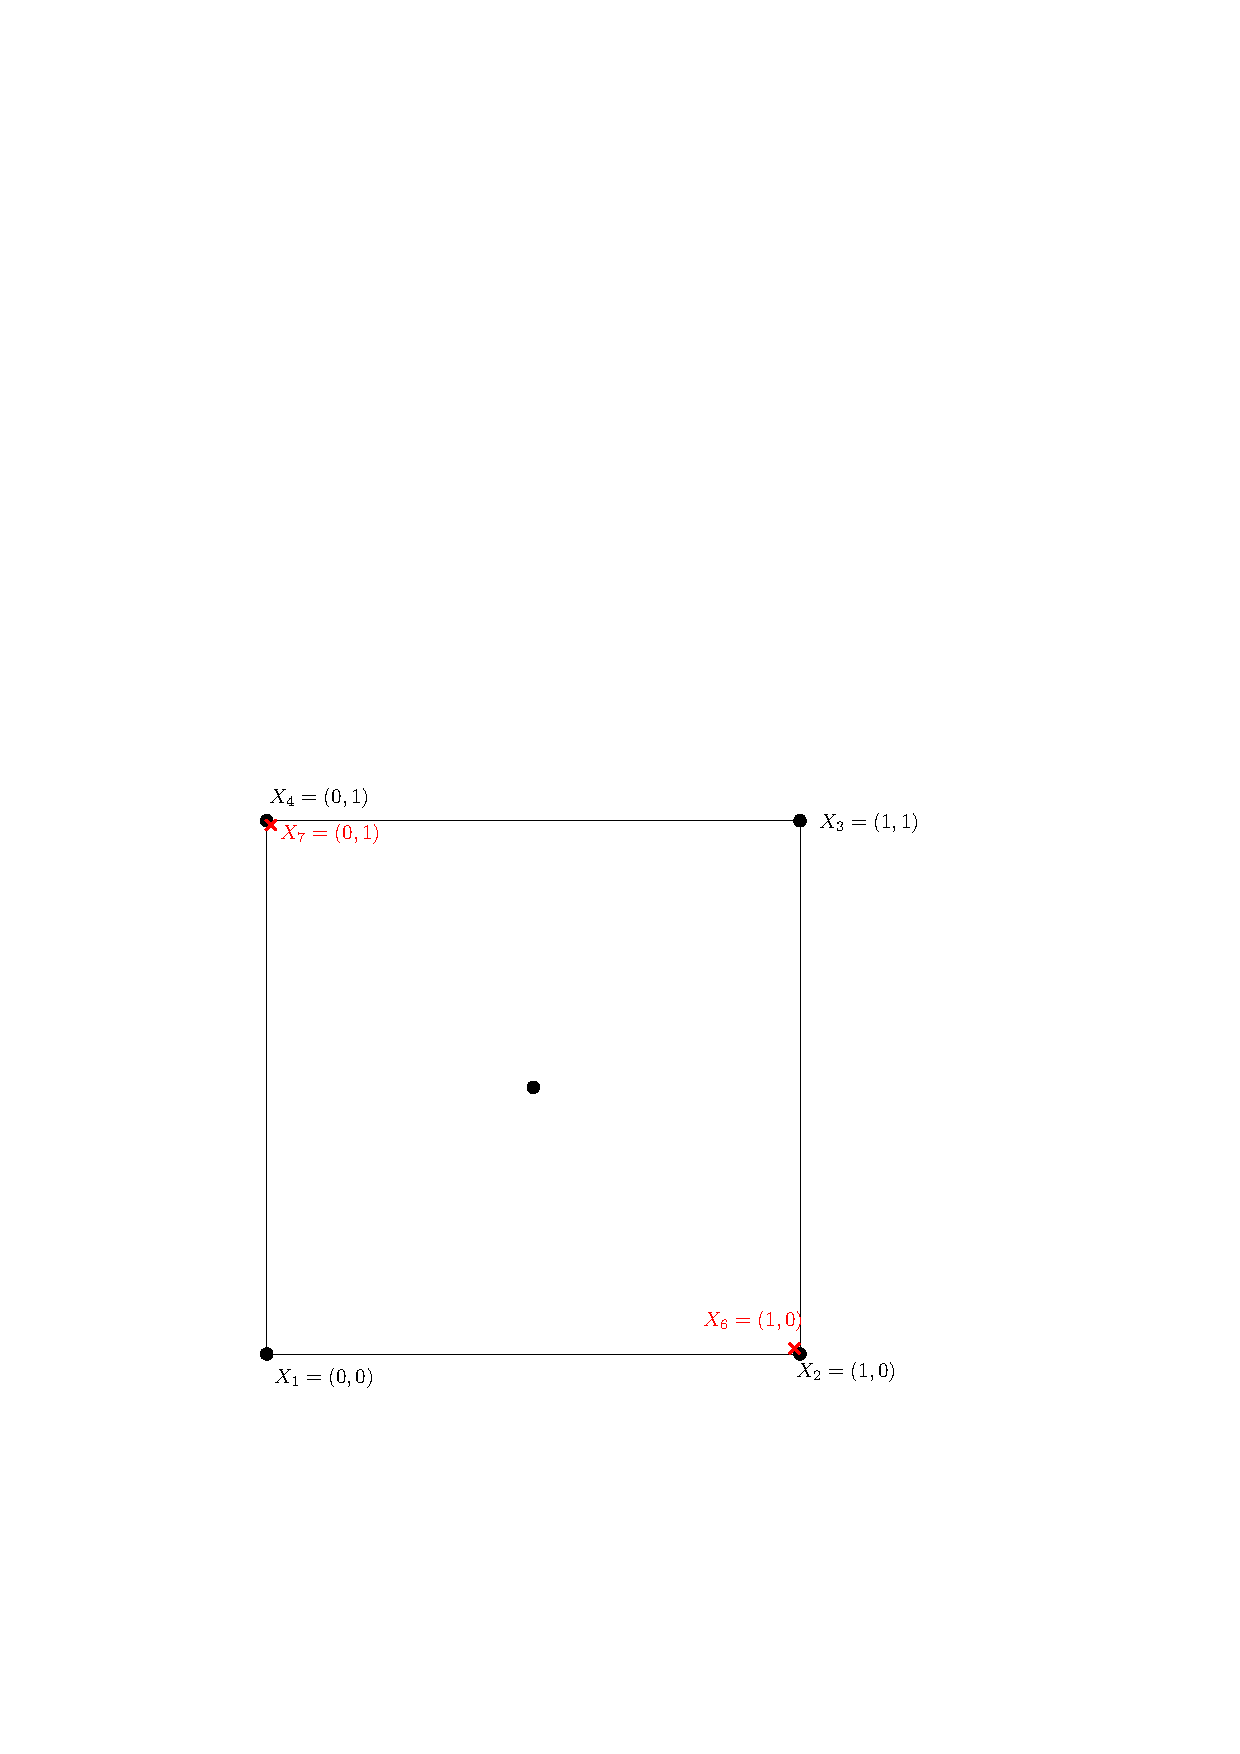
\includegraphics{multmin-diag}
 \end{figure} 
  Suppose $X_6$ is matched with $X_2$ and $X_7$ is matched with $X_4$. 
  Denote the Euclidean distance matrix by $D$. 
  Suppose, due to noise, or due to dissimilarities not being Euclidean distances, 
  our dissimilarity matrix is $$D'_{ij}=\begin{cases}
  D_ij-1.4 & \textrm{if  $(i,j) \in \{(4,6),(6,4),(2,7),(7,2)   \}$ }\\
  D_ij  & \textrm{ otherwise}\\
  \end{cases}.$$ Qualitatively, the three points $X_1$, $X_7$ and $X_3$ form a barrier which   the OOS points need to cross  to reach their matched counterparts.
   
   Based on the initial configuration, the  embedding coordinates of $\hat{X}_6$ might be closer
    to $X_4$ compared to $X_2$. This is due to a local minimum in the configuration space.  If $\hat{X}_6$ starts from the initial configuration where it's located on the $X_4$ side of the y=x line at the start of optimization, 
    it might have to cross paths with the embedding of  ${X}_1,{X}_3,{X}_7$ with which it has a  nonzero dissimilarity.  
    Based on value of $w$, it might be easier to get out of this local minimum. 
    In fact, depending on w can this  local minimum can be a global minimum. 
    That is, the configuration where $X_6$ stays on the side of $X_4$ instead of $X_2$ might have a lower stress than the configuration where $X_6$ is near $X_2$. 
    The following plots shows the local minimum $\hat{X}_6$ ends up in, depending on initial configuration. 
    Depending on $w$ value, one of these minima has a lower weighted stress than the other.   


\begin{figure}
\begin{minipage}[b]{0.5\linewidth}
\centering
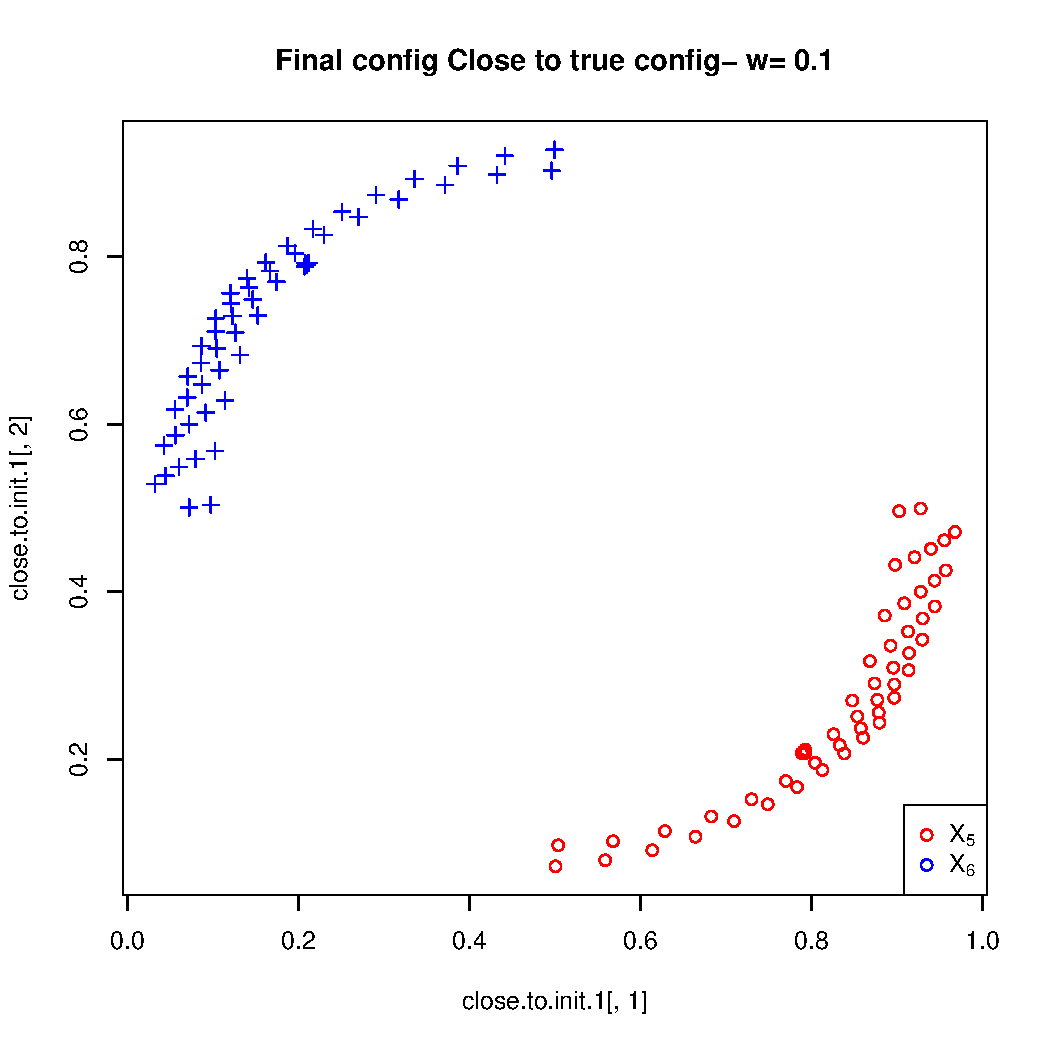
\includegraphics[scale=0.35]{true-min-w-0_1.pdf}

\label{fig:figure1-1}
\end{minipage}
\hspace{0.5cm}
\begin{minipage}[b]{0.5\linewidth}
\centering
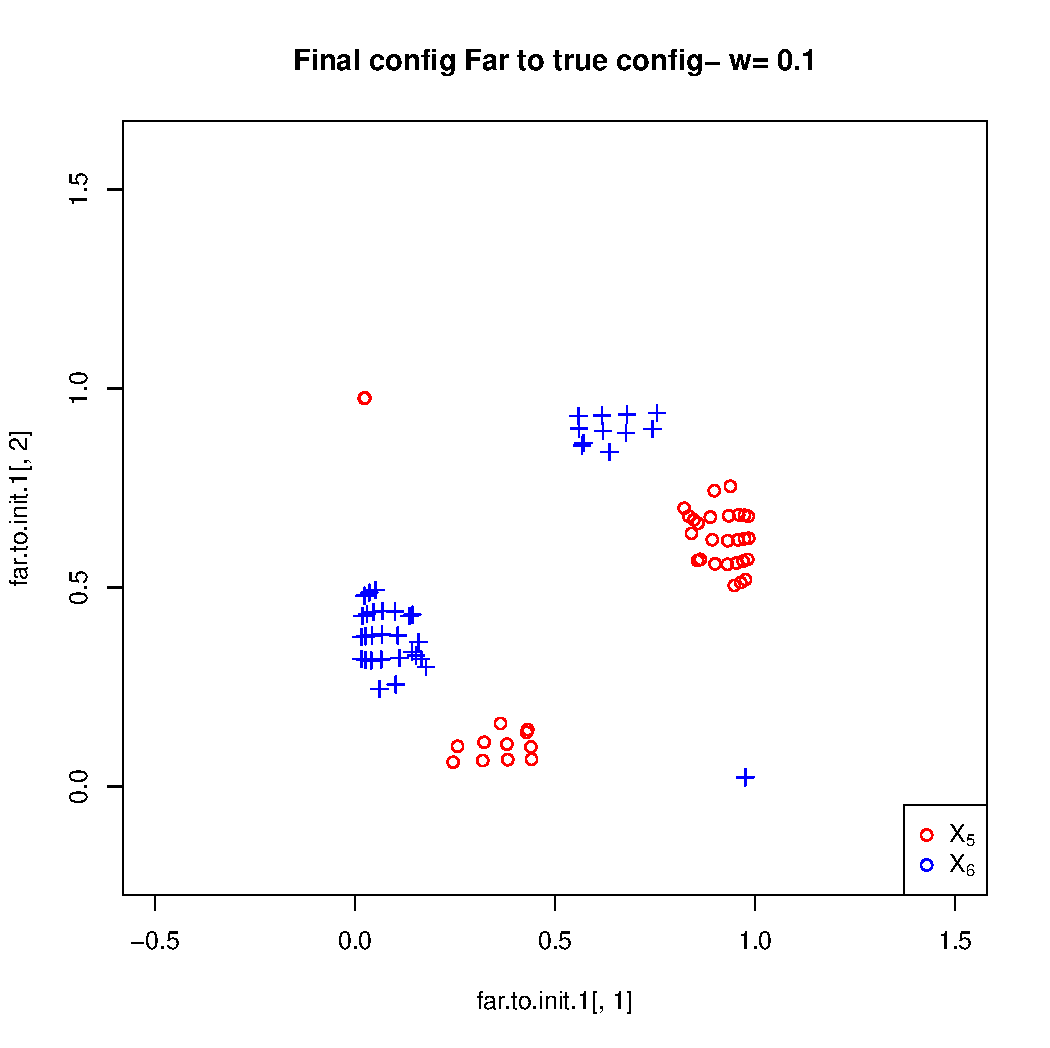
\includegraphics[scale=0.35]{other-min-w-0_1.pdf}

\label{fig:figure1-2}
\end{minipage}

\caption{Final configurations for for different $w=0.1$ }
\label{fig:Finalconfig-MultMin-w-0_1}

\end{figure}




\begin{figure}
\begin{minipage}[b]{0.5\linewidth}
\centering
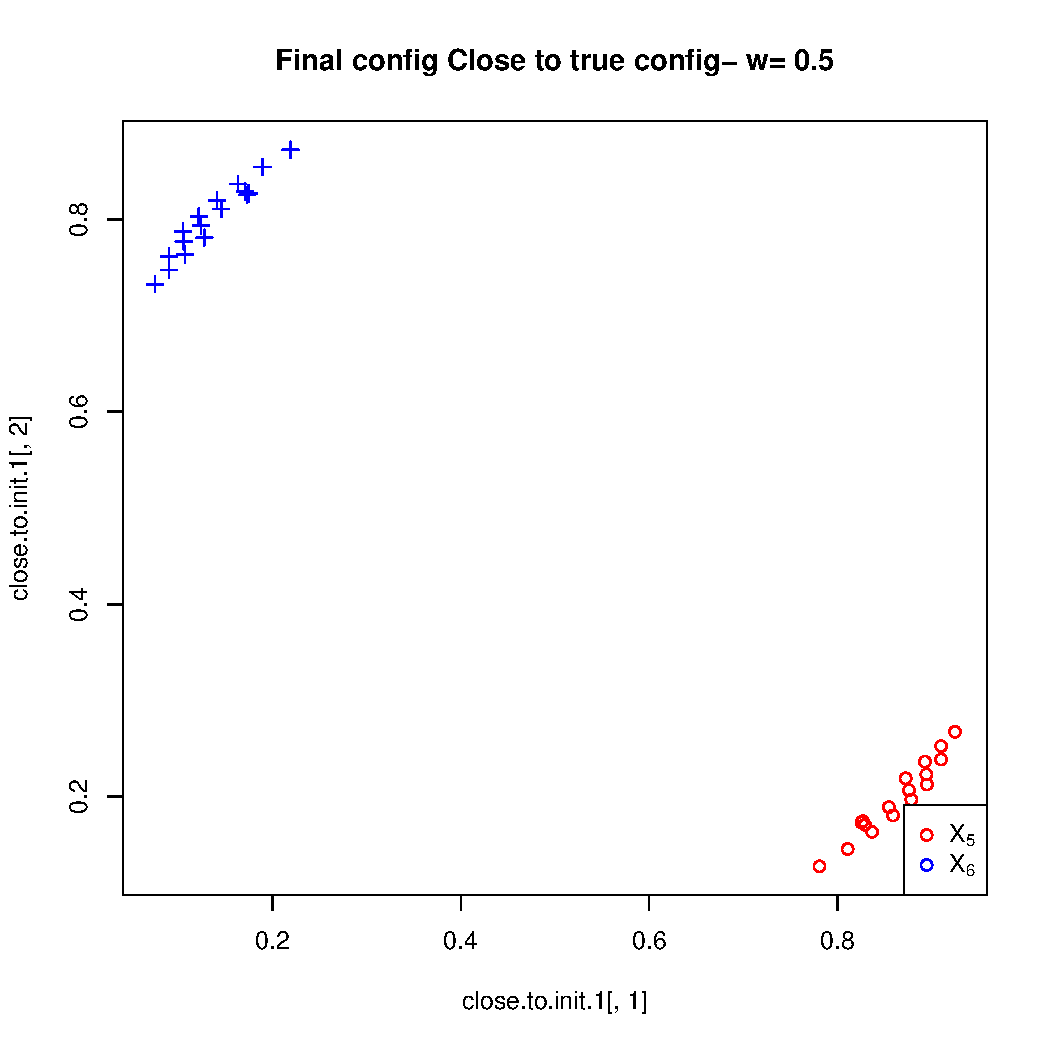
\includegraphics[scale=0.35]{true-min-w-0_5.pdf}

\label{fig:figure2-1}
\end{minipage}
\hspace{0.5cm}
\begin{minipage}[b]{0.5\linewidth}
\centering
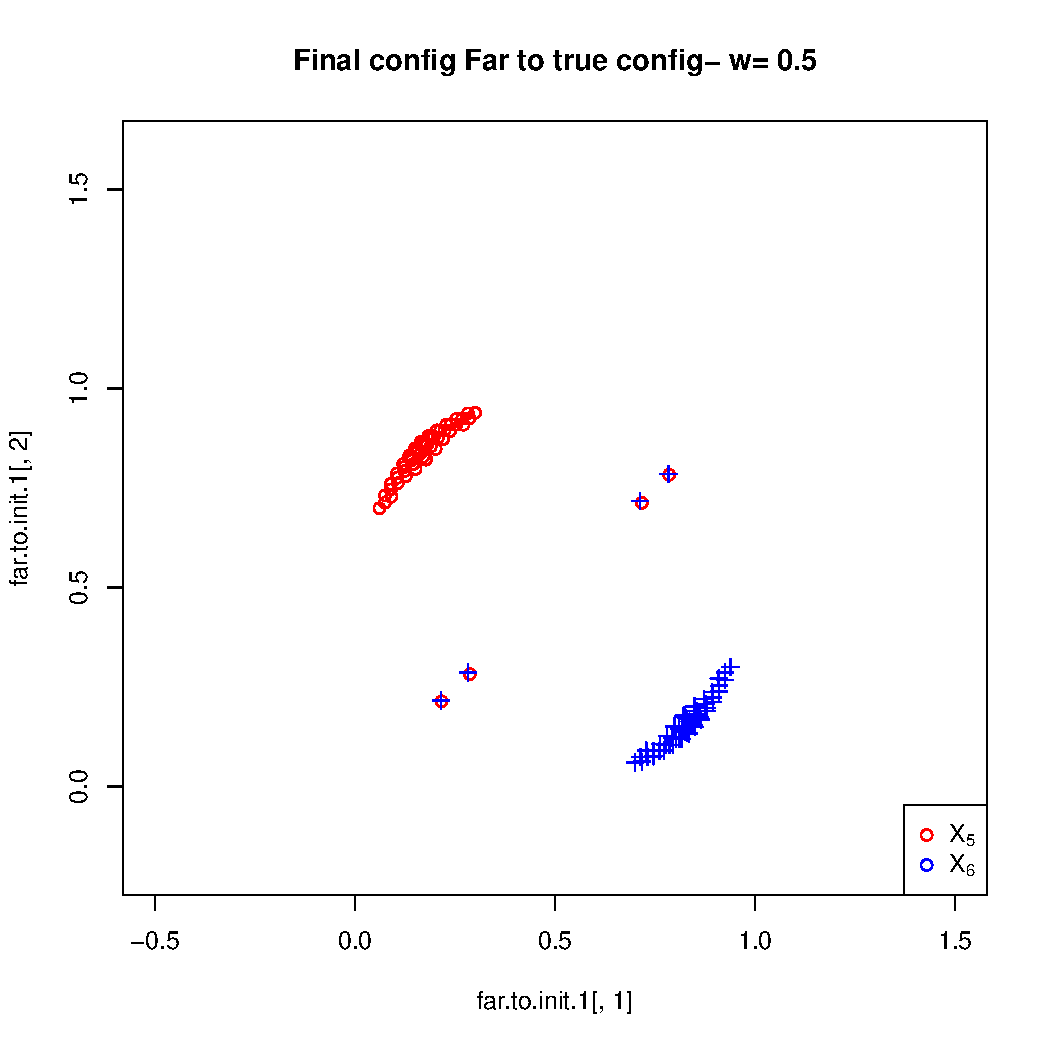
\includegraphics[scale=0.35]{other-min-w-0_5.pdf}

\label{fig:figure2-2}
\end{minipage}

\caption{Final configurations for for different $w=0.5$ }
\label{fig:Finalconfig-MultMin-w-0_5}

\end{figure}


\begin{figure}
\begin{minipage}[b]{0.5\linewidth}
\centering
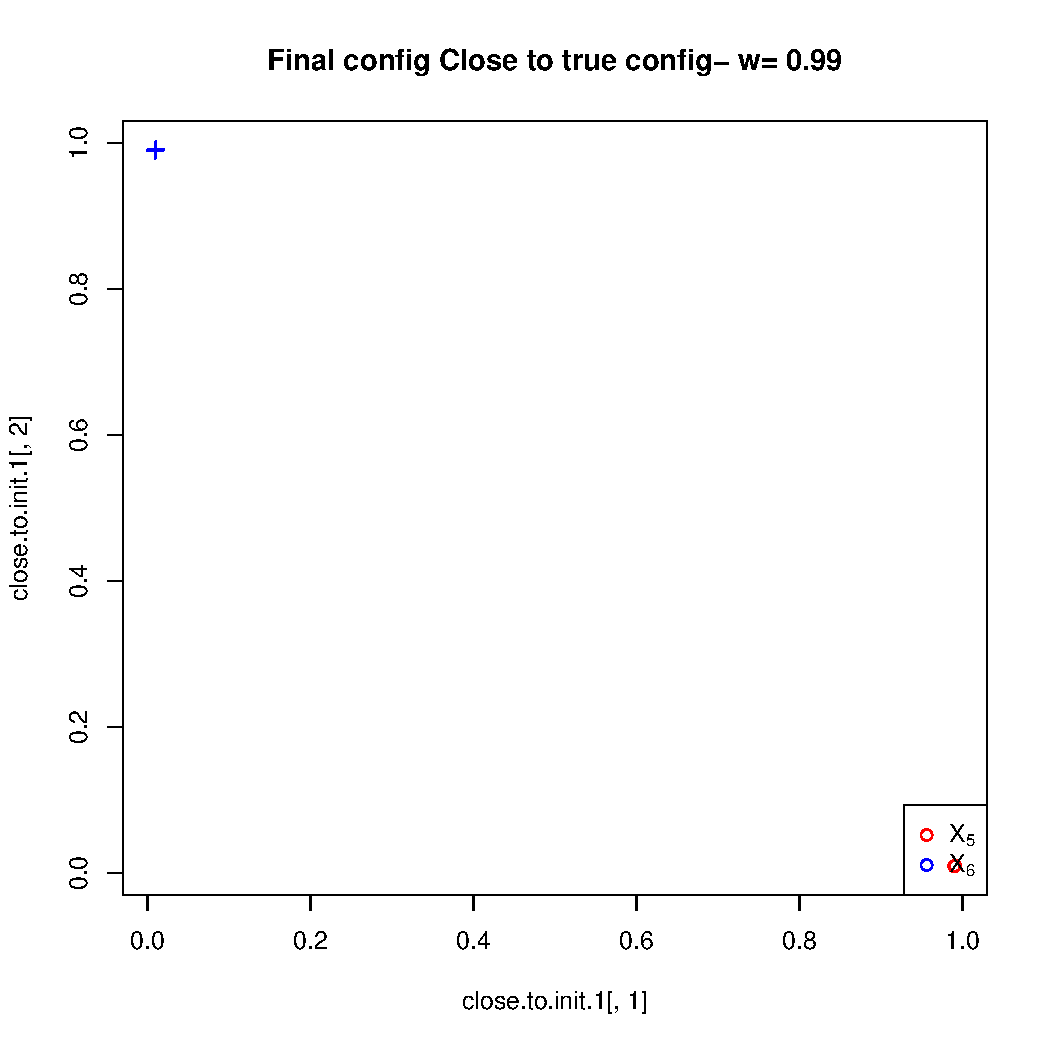
\includegraphics[scale=0.35]{true-min-w-0_99.pdf}

\label{fig:figure2-1}
\end{minipage}
\hspace{0.5cm}
\begin{minipage}[b]{0.5\linewidth}
\centering
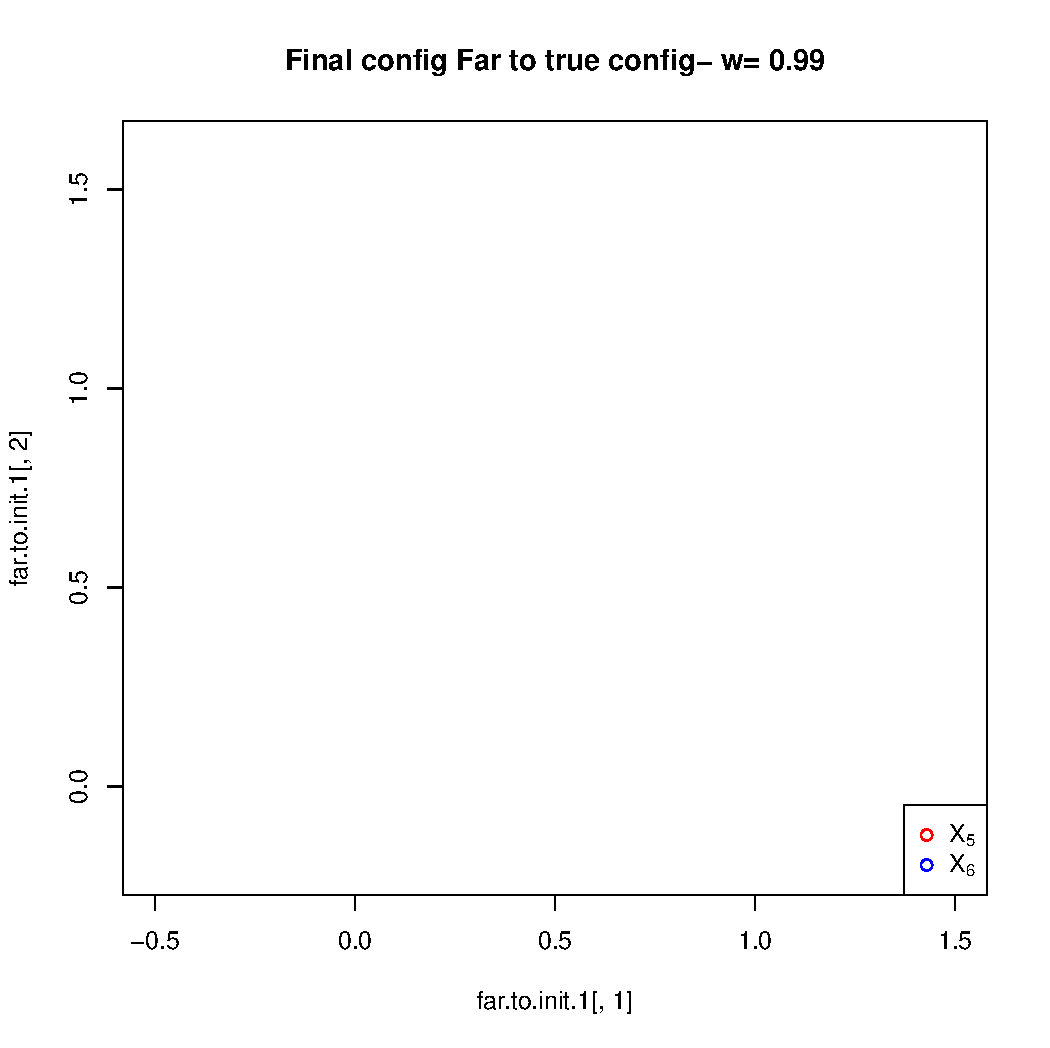
\includegraphics[scale=0.35]{other-min-w-0_99.pdf}

\label{fig:figure2-2}
\end{minipage}

\caption{Final configurations for for different $w=0.99$ }
\label{fig:Finalconfig-MultMin-w-0_99}

\end{figure}




% latex table generated in R 2.15.0 by xtable 1.7-0 package
% Wed Aug 08 01:28:55 2012
\begin{table}[ht]
\begin{center}
\begin{tabular}{rrrrrr}
  \hline
 & 0.1 & 0.45 & 0.5 & 0.55 & 0.99 \\ 
  \hline
Local min for real config. & 2.80 & 1.77 & 1.62 & 1.47 & 0.04 \\ 
  Alternative local min & 0.39 & 1.53 & 1.65 & 1.74 & 100.00 \\ 
   \hline
\end{tabular}
\end{center}
\end{table}


Other than such carefully constructed examples, we expect $w$ to have no effect on the ordering of the local minima according to their stress values.
Therefore,  the argmin among these local minima is independent of $w$. The minimum configuration is then a continuous function of $w$. 
By the continuity of the distance function with respect to configurations, the test statistic is continuous with respect to $w$. One can conclude $\beta(w) $ is a continuous function of $w$. 

 



\section{Simulation Results\label{sec:Simulation Results}}
To compare the  different approaches, training data of matched sets of measurements were generated according to the Dirichlet and Gaussian settings. Dissimilarity representations were generated from pairwise distances of measurements. A set of matched pairs of measurements and unmatched pairs of measurements were also generated for testing. The test statistics (computed via P$\circ $M, CCA and JOFC approaches) for matched and unmatched pairs were used to compute power values at a set of fixed type I error rate $\alpha$ values.

 Additionally, to take robustness of methods into consideration, ``noisy" measurements were created from the original measurements by concatenating randomly generated independent noise vectors (subsection \ref{noise}).   This setting will be referred to as the ``noisy case". The original setting, with $c=0$,  will be referred as the ``noiseless case".
If the magnitude of noise (controlled by the parameter $c$ in equation \eqref{eq:noise-expr}) is small enough, PCA and MDS will not be affected significantly, but if the number of noisy dimensions (controlled by the parameter $q$ in the distribution of $E_{ik}$ as defined in equation \eqref{eq:noise-expr}) is large enough, CCA  will be affected due to spurious correlation between noisy dimensions.

Given the setting ("Gaussian","Dirichlet"),   the steps for each Monte Carlo replicate are as follows:
\begin{itemize}
\item A training set ($\mathbf{T}_{mc}$) which consists of  $n$ pairs of matched measurements is generated.  If $c=0$, we are in the ``noiseless" setting and measurements are $p$-dimensional vectors, otherwise we are in the ``noisy" setting and measurement vectors are $(p+q)$-dimensional.
\item Dissimilarities are computed and embedded in  Euclidean space  via MDS (followed by a transformation from  $\mathbf{R}^d$ to  $\mathbf{R}^d$ and  projection into $\mathbf{R}^d$, respectively  for P$\circ$M and CCA) . The final embeddings lie in $\mathbb{R}^d$.   Denote this in-sample embedding as   $\hat{\mathbf{T}}$. Note that  if the JOFC method is being used, embedding is carried out with the weighted raw stress function $\sigma_{W}(\cdot)=f_{w}(D(\cdot),M)$ in equation \eqref{fid-comm-tradeoff-func} with a common weight $w$ for commensurability terms and another common weight $1-w$ for fidelity terms, otherwise unweighted raw stress function ($\sigma(\cdot)$) is used as a criterion function for embedding.

\item We generate $m$ pairs of matched   measurements  which we treat as out-of-sample, and 
\begin{itemize}
\item compute the dissimilarities  %$\mathbf{\Delta}^{new}={ \delta_{ik}^{new}; i=1,\ldots, n;\hspace{5pt} k=1,2}$
 between these out-of-sample  points and the points in ${\mathbf{T}_{mc}}$,  
\item  embed the OOS dissimilarities as pairs of embedded points via the OOS extension:\\
 $(\tilde{y}_1^{(1)},\tilde{y}_1^{(2)}),\ldots, (\tilde{y}_m^{(1)},\tilde{y}_m^{(2)})$, 
\item compute the test statistic $\tau$ for each pair.%, $t(\tilde{y}_i^{(1)},\tilde{y}_i^{(2)});\hspace{4pt}
%i=1,\ldots,m$
\end{itemize}
 The values of the statistic $\tau$ are used for computing  the empirical cumulative distribution function under null hypothesis. 

\item Identical steps for $m$ pairs of unmatched measurements result in the empirical cumulative distribution  function of $\tau$ under alternative hypothesis.
\item For any fixed $\alpha$ value, a critical value for the test statistic and the corresponding power is computed.
\end{itemize}

%<<sim-two-cond-pre-pre,cache=FALSE>>=
%setwd("G:/Users/Sancar/Documents/projects/DataFusion")
%@



\begin{Schunk}
\begin{Soutput}
[1] FALSE
[1] "2 150 0.01"
[1] "Gaussian Setting Simulation Starting, running simulate.generate.test.model.plot"
[1] "c"
[1] 0.01
[1] 3
[1] "w values"
[1] 0.500 0.800 0.850 0.900 0.925 0.950 0.990 0.999
R Version:  R version 2.15.0 (2012-03-30) 

[1] "Starting parallelization in gaussian_simulation_jofc_tradeoff_sf"
List of 13
 $ power.mc            : num [1:8, 1:101] 0 0 0 0 0 ...
 $ power.cmp           :List of 3
  ..$ cca    : num [1:101] 0 0.8 0.8 0.807 0.813 ...
  ..$ pom    : num [1:101] 0 0.727 0.747 0.78 0.787 ...
  ..$ cca.reg: NULL
 $ cont.tables         : num [1:2, 1:2] 0 0 0 0
 $ config.dist         :List of 1
  ..$ frob.norm: num [1:8(1d)] 0 0 0 0 0 0 0 0
 $ min.stress          : num [1:9] 0 0 0 0 0 0 0 0 0
 $ means               : num [1:8, 1:4] 0 0 0 0 0 0 0 0 0 0 ...
 $ FidComm.Terms       :List of 3
  ..$ F1: num [1:8] 0.211 0.213 0.214 0.217 0.219 ...
  ..$ F2: num [1:8] 0.194 0.196 0.198 0.201 0.205 ...
  ..$ C : num [1:8] 0.481 0.349 0.304 0.245 0.198 ...
 $ FidComm.Sum.Terms   :List of 3
  ..$ F1: num [1:8] 2358 2376 2390 2421 2449 ...
  ..$ F2: num [1:8] 2170 2193 2211 2244 2290 ...
  ..$ C : num [1:8] 72.1 52.3 45.7 36.7 29.7 ...
 $ F.to.C.ratio        : num [1:8] 62.8 87.4 100.8 127 159.8 ...
 $ wtF.to.C.ratio      : num [1:8] 62.8 21.8 17.8 14.1 13 ...
 $ F.bar.to.C.bar.ratio: num [1:8] 0.843 1.173 1.353 1.704 2.145 ...
 $ optim.power         : num [1:101] 0 0.794 0.827 0.846 0.86 ...
 $ best.w              : num 0.9
NULL
[1] "1 th contingency table"
     [,1] [,2]
[1,]    0    0
[2,]    0    0
List of 13
 $ power.mc            : num [1:8, 1:101] 0 0 0 0 0 ...
 $ power.cmp           :List of 3
  ..$ cca    : num [1:101] 0 0.8 0.82 0.82 0.853 ...
  ..$ pom    : num [1:101] 0 0.62 0.62 0.673 0.68 ...
  ..$ cca.reg: NULL
 $ cont.tables         : num [1:2, 1:2] 0 0 0 0
 $ config.dist         :List of 1
  ..$ frob.norm: num [1:8(1d)] 0 0 0 0 0 0 0 0
 $ min.stress          : num [1:9] 0 0 0 0 0 0 0 0 0
 $ means               : num [1:8, 1:4] 0 0 0 0 0 0 0 0 0 0 ...
 $ FidComm.Terms       :List of 3
  ..$ F1: num [1:8] 0.266 0.269 0.27 0.271 0.273 ...
  ..$ F2: num [1:8] 0.255 0.259 0.261 0.259 0.261 ...
  ..$ C : num [1:8] 0.615 0.332 0.285 0.174 0.145 ...
 $ FidComm.Sum.Terms   :List of 3
  ..$ F1: num [1:8] 2968 3005 3019 3029 3051 ...
  ..$ F2: num [1:8] 2852 2894 2914 2897 2922 ...
  ..$ C : num [1:8] 92.3 49.7 42.7 26.1 21.7 ...
 $ F.to.C.ratio        : num [1:8] 63 119 139 227 275 ...
 $ wtF.to.C.ratio      : num [1:8] 63 29.7 24.5 25.3 22.3 ...
 $ F.bar.to.C.bar.ratio: num [1:8] 0.846 1.592 1.866 3.05 3.694 ...
 $ optim.power         : num [1:101] 0 0.794 0.827 0.846 0.86 ...
 $ best.w              : num 0.95
NULL
[1] "2 th contingency table"
     [,1] [,2]
[1,]    0    0
[2,]    0    0
List of 13
 $ power.mc            : num [1:8, 1:101] 0 0 0 0 0 ...
 $ power.cmp           :List of 3
  ..$ cca    : num [1:101] 0 0.507 0.52 0.54 0.62 ...
  ..$ pom    : num [1:101] 0 0.66 0.7 0.72 0.733 ...
  ..$ cca.reg: NULL
 $ cont.tables         : num [1:2, 1:2] 0 0 0 0
 $ config.dist         :List of 1
  ..$ frob.norm: num [1:8(1d)] 0 0 0 0 0 0 0 0
 $ min.stress          : num [1:9] 0 0 0 0 0 0 0 0 0
 $ means               : num [1:8, 1:4] 0 0 0 0 0 0 0 0 0 0 ...
 $ FidComm.Terms       :List of 3
  ..$ F1: num [1:8] 0.231 0.236 0.236 0.24 0.241 ...
  ..$ F2: num [1:8] 0.232 0.233 0.237 0.238 0.243 ...
  ..$ C : num [1:8] 0.563 0.323 0.273 0.205 0.171 ...
 $ FidComm.Sum.Terms   :List of 3
  ..$ F1: num [1:8] 2577 2639 2642 2681 2694 ...
  ..$ F2: num [1:8] 2588 2609 2649 2656 2711 ...
  ..$ C : num [1:8] 84.5 48.4 40.9 30.7 25.7 ...
 $ F.to.C.ratio        : num [1:8] 61.1 108.3 129.2 173.7 210.6 ...
 $ wtF.to.C.ratio      : num [1:8] 61.1 27.1 22.8 19.3 17.1 ...
 $ F.bar.to.C.bar.ratio: num [1:8] 0.82 1.45 1.73 2.33 2.83 ...
 $ optim.power         : num [1:101] 0 0.794 0.827 0.846 0.86 ...
 $ best.w              : num 0.95
NULL
[1] "3 th contingency table"
     [,1] [,2]
[1,]    0    0
[2,]    0    0
List of 13
 $ power.mc            : num [1:8, 1:101] 0 0 0 0 0 ...
 $ power.cmp           :List of 3
  ..$ cca    : num [1:101] 0 0.793 0.793 0.8 0.807 ...
  ..$ pom    : num [1:101] 0 0.587 0.66 0.66 0.687 ...
  ..$ cca.reg: NULL
 $ cont.tables         : num [1:2, 1:2] 0 0 0 0
 $ config.dist         :List of 1
  ..$ frob.norm: num [1:8(1d)] 0 0 0 0 0 0 0 0
 $ min.stress          : num [1:9] 0 0 0 0 0 0 0 0 0
 $ means               : num [1:8, 1:4] 0 0 0 0 0 0 0 0 0 0 ...
 $ FidComm.Terms       :List of 3
  ..$ F1: num [1:8] 0.253 0.256 0.256 0.259 0.262 ...
  ..$ F2: num [1:8] 0.247 0.253 0.257 0.259 0.262 ...
  ..$ C : num [1:8] 0.648 0.36 0.245 0.189 0.153 ...
 $ FidComm.Sum.Terms   :List of 3
  ..$ F1: num [1:8] 2832 2862 2866 2896 2924 ...
  ..$ F2: num [1:8] 2764 2822 2868 2898 2927 ...
  ..$ C : num [1:8] 97.2 53.9 36.8 28.4 22.9 ...
 $ F.to.C.ratio        : num [1:8] 57.6 105.4 155.9 204.3 255.3 ...
 $ wtF.to.C.ratio      : num [1:8] 57.6 26.3 27.5 22.7 20.7 ...
 $ F.bar.to.C.bar.ratio: num [1:8] 0.773 1.414 2.092 2.743 3.427 ...
 $ optim.power         : num [1:101] 0 0.794 0.827 0.846 0.86 ...
 $ best.w              : num 0.925
NULL
[1] "4 th contingency table"
     [,1] [,2]
[1,]    0    0
[2,]    0    0
List of 13
 $ power.mc            : num [1:8, 1:101] 0 0 0 0 0 ...
 $ power.cmp           :List of 3
  ..$ cca    : num [1:101] 0 0.76 0.767 0.767 0.78 ...
  ..$ pom    : num [1:101] 0 0.7 0.7 0.753 0.773 ...
  ..$ cca.reg: NULL
 $ cont.tables         : num [1:2, 1:2] 0 0 0 0
 $ config.dist         :List of 1
  ..$ frob.norm: num [1:8(1d)] 0 0 0 0 0 0 0 0
 $ min.stress          : num [1:9] 0 0 0 0 0 0 0 0 0
 $ means               : num [1:8, 1:4] 0 0 0 0 0 0 0 0 0 0 ...
 $ FidComm.Terms       :List of 3
  ..$ F1: num [1:8] 0.267 0.269 0.27 0.272 0.276 ...
  ..$ F2: num [1:8] 0.22 0.223 0.224 0.227 0.229 ...
  ..$ C : num [1:8] 0.511 0.327 0.29 0.235 0.192 ...
 $ FidComm.Sum.Terms   :List of 3
  ..$ F1: num [1:8] 2982 3001 3015 3045 3084 ...
  ..$ F2: num [1:8] 2464 2491 2505 2535 2564 ...
  ..$ C : num [1:8] 76.7 49 43.5 35.2 28.8 ...
 $ F.to.C.ratio        : num [1:8] 71 112 127 159 196 ...
 $ wtF.to.C.ratio      : num [1:8] 71 28 22.4 17.6 15.9 ...
 $ F.bar.to.C.bar.ratio: num [1:8] 0.954 1.503 1.705 2.128 2.632 ...
 $ optim.power         : num [1:101] 0 0.794 0.827 0.846 0.86 ...
 $ best.w              : num 0.925
NULL
[1] "5 th contingency table"
     [,1] [,2]
[1,]    0    0
[2,]    0    0
List of 13
 $ power.mc            : num [1:8, 1:101] 0 0 0 0 0 ...
 $ power.cmp           :List of 3
  ..$ cca    : num [1:101] 0 0.7 0.72 0.733 0.74 ...
  ..$ pom    : num [1:101] 0 0.54 0.627 0.627 0.687 ...
  ..$ cca.reg: NULL
 $ cont.tables         : num [1:2, 1:2] 0 0 0 0
 $ config.dist         :List of 1
  ..$ frob.norm: num [1:8(1d)] 0 0 0 0 0 0 0 0
 $ min.stress          : num [1:9] 0 0 0 0 0 0 0 0 0
 $ means               : num [1:8, 1:4] 0 0 0 0 0 0 0 0 0 0 ...
 $ FidComm.Terms       :List of 3
  ..$ F1: num [1:8] 0.25 0.252 0.253 0.257 0.259 ...
  ..$ F2: num [1:8] 0.214 0.218 0.219 0.221 0.224 ...
  ..$ C : num [1:8] 0.489 0.326 0.284 0.22 0.183 ...
 $ FidComm.Sum.Terms   :List of 3
  ..$ F1: num [1:8] 2796 2814 2829 2868 2898 ...
  ..$ F2: num [1:8] 2395 2432 2448 2474 2504 ...
  ..$ C : num [1:8] 73.4 48.9 42.6 33.1 27.5 ...
 $ F.to.C.ratio        : num [1:8] 70.7 107.2 123.9 161.6 196.7 ...
 $ wtF.to.C.ratio      : num [1:8] 70.7 26.8 21.9 18 16 ...
 $ F.bar.to.C.bar.ratio: num [1:8] 0.95 1.44 1.66 2.17 2.64 ...
 $ optim.power         : num [1:101] 0 0.794 0.827 0.846 0.86 ...
 $ best.w              : num 0.95
NULL
[1] "6 th contingency table"
     [,1] [,2]
[1,]    0    0
[2,]    0    0
List of 13
 $ power.mc            : num [1:8, 1:101] 0 0 0 0 0 ...
 $ power.cmp           :List of 3
  ..$ cca    : num [1:101] 0 0.767 0.767 0.767 0.793 ...
  ..$ pom    : num [1:101] 0 0.773 0.793 0.84 0.847 ...
  ..$ cca.reg: NULL
 $ cont.tables         : num [1:2, 1:2] 0 0 0 0
 $ config.dist         :List of 1
  ..$ frob.norm: num [1:8(1d)] 0 0 0 0 0 0 0 0
 $ min.stress          : num [1:9] 0 0 0 0 0 0 0 0 0
 $ means               : num [1:8, 1:4] 0 0 0 0 0 0 0 0 0 0 ...
 $ FidComm.Terms       :List of 3
  ..$ F1: num [1:8] 0.215 0.217 0.219 0.223 0.227 ...
  ..$ F2: num [1:8] 0.221 0.222 0.224 0.227 0.228 ...
  ..$ C : num [1:8] 0.451 0.329 0.278 0.189 0.142 ...
 $ FidComm.Sum.Terms   :List of 3
  ..$ F1: num [1:8] 2401 2425 2445 2488 2542 ...
  ..$ F2: num [1:8] 2465 2483 2498 2533 2549 ...
  ..$ C : num [1:8] 67.7 49.4 41.7 28.3 21.2 ...
 $ F.to.C.ratio        : num [1:8] 71.9 99.4 118.4 177.4 239.6 ...
 $ wtF.to.C.ratio      : num [1:8] 71.9 24.9 20.9 19.7 19.4 ...
 $ F.bar.to.C.bar.ratio: num [1:8] 0.965 1.335 1.589 2.382 3.217 ...
 $ optim.power         : num [1:101] 0 0.794 0.827 0.846 0.86 ...
 $ best.w              : num 0.925
NULL
[1] "7 th contingency table"
     [,1] [,2]
[1,]    0    0
[2,]    0    0
List of 13
 $ power.mc            : num [1:8, 1:101] 0 0 0 0 0 ...
 $ power.cmp           :List of 3
  ..$ cca    : num [1:101] 0 0.773 0.793 0.8 0.847 ...
  ..$ pom    : num [1:101] 0 0.0733 0.1133 0.1333 0.1733 ...
  ..$ cca.reg: NULL
 $ cont.tables         : num [1:2, 1:2] 0 0 0 0
 $ config.dist         :List of 1
  ..$ frob.norm: num [1:8(1d)] 0 0 0 0 0 0 0 0
 $ min.stress          : num [1:9] 0 0 0 0 0 0 0 0 0
 $ means               : num [1:8, 1:4] 0 0 0 0 0 0 0 0 0 0 ...
 $ FidComm.Terms       :List of 3
  ..$ F1: num [1:8] 0.239 0.258 0.263 0.242 0.243 ...
  ..$ F2: num [1:8] 0.245 0.255 0.264 0.261 0.263 ...
  ..$ C : num [1:8] 2.0379 0.9186 0.2439 0.1139 0.0926 ...
 $ FidComm.Sum.Terms   :List of 3
  ..$ F1: num [1:8] 2670 2883 2941 2699 2713 ...
  ..$ F2: num [1:8] 2732 2855 2951 2916 2936 ...
  ..$ C : num [1:8] 305.7 137.8 36.6 17.1 13.9 ...
 $ F.to.C.ratio        : num [1:8] 17.7 41.6 161 328.7 406.7 ...
 $ wtF.to.C.ratio      : num [1:8] 17.7 10.4 28.4 36.5 33 ...
 $ F.bar.to.C.bar.ratio: num [1:8] 0.237 0.559 2.162 4.412 5.46 ...
 $ optim.power         : num [1:101] 0 0.794 0.827 0.846 0.86 ...
 $ best.w              : num 0.925
NULL
[1] "8 th contingency table"
     [,1] [,2]
[1,]    0    0
[2,]    0    0
List of 13
 $ power.mc            : num [1:8, 1:101] 0 0 0 0 0 ...
 $ power.cmp           :List of 3
  ..$ cca    : num [1:101] 0 0.68 0.707 0.72 0.727 ...
  ..$ pom    : num [1:101] 0 0.6 0.653 0.653 0.687 ...
  ..$ cca.reg: NULL
 $ cont.tables         : num [1:2, 1:2] 0 0 0 0
 $ config.dist         :List of 1
  ..$ frob.norm: num [1:8(1d)] 0 0 0 0 0 0 0 0
 $ min.stress          : num [1:9] 0 0 0 0 0 0 0 0 0
 $ means               : num [1:8, 1:4] 0 0 0 0 0 0 0 0 0 0 ...
 $ FidComm.Terms       :List of 3
  ..$ F1: num [1:8] 0.288 0.287 0.288 0.29 0.292 ...
  ..$ F2: num [1:8] 0.262 0.265 0.266 0.268 0.27 ...
  ..$ C : num [1:8] 0.739 0.27 0.241 0.197 0.164 ...
 $ FidComm.Sum.Terms   :List of 3
  ..$ F1: num [1:8] 3220 3204 3216 3240 3265 ...
  ..$ F2: num [1:8] 2925 2962 2972 2995 3021 ...
  ..$ C : num [1:8] 110.8 40.5 36.1 29.6 24.6 ...
 $ F.to.C.ratio        : num [1:8] 55.4 152.2 171.5 210.9 255.4 ...
 $ wtF.to.C.ratio      : num [1:8] 55.4 38.1 30.3 23.4 20.7 ...
 $ F.bar.to.C.bar.ratio: num [1:8] 0.744 2.043 2.302 2.831 3.428 ...
 $ optim.power         : num [1:101] 0 0.794 0.827 0.846 0.86 ...
 $ best.w              : num 0.925
NULL
[1] "9 th contingency table"
     [,1] [,2]
[1,]    0    0
[2,]    0    0
List of 13
 $ power.mc            : num [1:8, 1:101] 0 0 0 0 0 ...
 $ power.cmp           :List of 3
  ..$ cca    : num [1:101] 0 0.827 0.853 0.867 0.867 ...
  ..$ pom    : num [1:101] 0 0.64 0.72 0.74 0.747 ...
  ..$ cca.reg: NULL
 $ cont.tables         : num [1:2, 1:2] 0 0 0 0
 $ config.dist         :List of 1
  ..$ frob.norm: num [1:8(1d)] 0 0 0 0 0 0 0 0
 $ min.stress          : num [1:9] 0 0 0 0 0 0 0 0 0
 $ means               : num [1:8, 1:4] 0 0 0 0 0 0 0 0 0 0 ...
 $ FidComm.Terms       :List of 3
  ..$ F1: num [1:8] 0.238 0.243 0.243 0.245 0.247 ...
  ..$ F2: num [1:8] 0.245 0.246 0.247 0.249 0.251 ...
  ..$ C : num [1:8] 0.529 0.271 0.225 0.183 0.154 ...
 $ FidComm.Sum.Terms   :List of 3
  ..$ F1: num [1:8] 2657 2712 2715 2736 2758 ...
  ..$ F2: num [1:8] 2735 2751 2759 2783 2808 ...
  ..$ C : num [1:8] 79.3 40.7 33.7 27.5 23 ...
 $ F.to.C.ratio        : num [1:8] 68 134 162 201 242 ...
 $ wtF.to.C.ratio      : num [1:8] 68 33.6 28.7 22.3 19.6 ...
 $ F.bar.to.C.bar.ratio: num [1:8] 0.912 1.801 2.18 2.695 3.242 ...
 $ optim.power         : num [1:101] 0 0.794 0.827 0.846 0.86 ...
 $ best.w              : num 0.95
NULL
[1] "10 th contingency table"
     [,1] [,2]
[1,]    0    0
[2,]    0    0
List of 13
 $ power.mc            : num [1:8, 1:101] 0 0 0 0 0 ...
 $ power.cmp           :List of 3
  ..$ cca    : num [1:101] 0 0.82 0.827 0.84 0.9 ...
  ..$ pom    : num [1:101] 0 0.733 0.733 0.753 0.767 ...
  ..$ cca.reg: NULL
 $ cont.tables         : num [1:2, 1:2] 0 0 0 0
 $ config.dist         :List of 1
  ..$ frob.norm: num [1:8(1d)] 0 0 0 0 0 0 0 0
 $ min.stress          : num [1:9] 0 0 0 0 0 0 0 0 0
 $ means               : num [1:8, 1:4] 0 0 0 0 0 0 0 0 0 0 ...
 $ FidComm.Terms       :List of 3
  ..$ F1: num [1:8] 0.18 0.181 0.182 0.184 0.185 ...
  ..$ F2: num [1:8] 0.185 0.185 0.186 0.188 0.19 ...
  ..$ C : num [1:8] 0.33 0.204 0.179 0.143 0.12 ...
 $ FidComm.Sum.Terms   :List of 3
  ..$ F1: num [1:8] 2016 2025 2033 2052 2070 ...
  ..$ F2: num [1:8] 2063 2073 2082 2102 2122 ...
  ..$ C : num [1:8] 49.4 30.6 26.9 21.5 18 ...
 $ F.to.C.ratio        : num [1:8] 82.5 133.9 153.1 193.2 233.3 ...
 $ wtF.to.C.ratio      : num [1:8] 82.5 33.5 27 21.5 18.9 ...
 $ F.bar.to.C.bar.ratio: num [1:8] 1.11 1.8 2.06 2.59 3.13 ...
 $ optim.power         : num [1:101] 0 0.794 0.827 0.846 0.86 ...
 $ best.w              : num 0.925
NULL
[1] "11 th contingency table"
     [,1] [,2]
[1,]    0    0
[2,]    0    0
List of 13
 $ power.mc            : num [1:8, 1:101] 0 0 0 0 0 ...
 $ power.cmp           :List of 3
  ..$ cca    : num [1:101] 0 0.767 0.787 0.813 0.827 ...
  ..$ pom    : num [1:101] 0 0.187 0.213 0.307 0.453 ...
  ..$ cca.reg: NULL
 $ cont.tables         : num [1:2, 1:2] 0 0 0 0
 $ config.dist         :List of 1
  ..$ frob.norm: num [1:8(1d)] 0 0 0 0 0 0 0 0
 $ min.stress          : num [1:9] 0 0 0 0 0 0 0 0 0
 $ means               : num [1:8, 1:4] 0 0 0 0 0 0 0 0 0 0 ...
 $ FidComm.Terms       :List of 3
  ..$ F1: num [1:8] 0.282 0.288 0.284 0.286 0.289 ...
  ..$ F2: num [1:8] 0.296 0.308 0.301 0.304 0.307 ...
  ..$ C : num [1:8] 1.493 0.581 0.256 0.202 0.166 ...
 $ FidComm.Sum.Terms   :List of 3
  ..$ F1: num [1:8] 3149 3219 3173 3199 3227 ...
  ..$ F2: num [1:8] 3306 3439 3363 3401 3428 ...
  ..$ C : num [1:8] 224 87.2 38.5 30.3 25 ...
 $ F.to.C.ratio        : num [1:8] 28.8 76.4 169.9 217.9 266.6 ...
 $ wtF.to.C.ratio      : num [1:8] 28.8 19.1 30 24.2 21.6 ...
 $ F.bar.to.C.bar.ratio: num [1:8] 0.387 1.025 2.28 2.925 3.579 ...
 $ optim.power         : num [1:101] 0 0.794 0.827 0.846 0.86 ...
 $ best.w              : num 0.95
NULL
[1] "12 th contingency table"
     [,1] [,2]
[1,]    0    0
[2,]    0    0
List of 13
 $ power.mc            : num [1:8, 1:101] 0 0 0 0 0 ...
 $ power.cmp           :List of 3
  ..$ cca    : num [1:101] 0 0.813 0.82 0.833 0.84 ...
  ..$ pom    : num [1:101] 0 0.76 0.8 0.807 0.833 ...
  ..$ cca.reg: NULL
 $ cont.tables         : num [1:2, 1:2] 0 0 0 0
 $ config.dist         :List of 1
  ..$ frob.norm: num [1:8(1d)] 0 0 0 0 0 0 0 0
 $ min.stress          : num [1:9] 0 0 0 0 0 0 0 0 0
 $ means               : num [1:8, 1:4] 0 0 0 0 0 0 0 0 0 0 ...
 $ FidComm.Terms       :List of 3
  ..$ F1: num [1:8] 0.234 0.235 0.236 0.238 0.239 ...
  ..$ F2: num [1:8] 0.247 0.249 0.251 0.253 0.255 ...
  ..$ C : num [1:8] 0.381 0.238 0.191 0.147 0.122 ...
 $ FidComm.Sum.Terms   :List of 3
  ..$ F1: num [1:8] 2614 2630 2639 2654 2672 ...
  ..$ F2: num [1:8] 2758 2785 2802 2832 2853 ...
  ..$ C : num [1:8] 57.1 35.7 28.6 22 18.3 ...
 $ F.to.C.ratio        : num [1:8] 94 152 190 249 301 ...
 $ wtF.to.C.ratio      : num [1:8] 94 37.9 33.5 27.7 24.4 ...
 $ F.bar.to.C.bar.ratio: num [1:8] 1.26 2.04 2.55 3.34 4.04 ...
 $ optim.power         : num [1:101] 0 0.794 0.827 0.846 0.86 ...
 $ best.w              : num 0.9
NULL
[1] "13 th contingency table"
     [,1] [,2]
[1,]    0    0
[2,]    0    0
List of 13
 $ power.mc            : num [1:8, 1:101] 0 0 0 0 0 ...
 $ power.cmp           :List of 3
  ..$ cca    : num [1:101] 0 0.693 0.7 0.78 0.793 ...
  ..$ pom    : num [1:101] 0 0.773 0.773 0.773 0.82 ...
  ..$ cca.reg: NULL
 $ cont.tables         : num [1:2, 1:2] 0 0 0 0
 $ config.dist         :List of 1
  ..$ frob.norm: num [1:8(1d)] 0 0 0 0 0 0 0 0
 $ min.stress          : num [1:9] 0 0 0 0 0 0 0 0 0
 $ means               : num [1:8, 1:4] 0 0 0 0 0 0 0 0 0 0 ...
 $ FidComm.Terms       :List of 3
  ..$ F1: num [1:8] 0.237 0.238 0.239 0.242 0.244 ...
  ..$ F2: num [1:8] 0.264 0.265 0.266 0.268 0.271 ...
  ..$ C : num [1:8] 0.432 0.278 0.24 0.193 0.16 ...
 $ FidComm.Sum.Terms   :List of 3
  ..$ F1: num [1:8] 2647 2661 2674 2700 2728 ...
  ..$ F2: num [1:8] 2953 2965 2975 3000 3025 ...
  ..$ C : num [1:8] 64.8 41.7 36 29 24 ...
 $ F.to.C.ratio        : num [1:8] 86.4 135 157.1 196.7 239.9 ...
 $ wtF.to.C.ratio      : num [1:8] 86.4 33.8 27.7 21.9 19.4 ...
 $ F.bar.to.C.bar.ratio: num [1:8] 1.16 1.81 2.11 2.64 3.22 ...
 $ optim.power         : num [1:101] 0 0.794 0.827 0.846 0.86 ...
 $ best.w              : num 0.95
NULL
[1] "14 th contingency table"
     [,1] [,2]
[1,]    0    0
[2,]    0    0
List of 13
 $ power.mc            : num [1:8, 1:101] 0 0 0 0 0 ...
 $ power.cmp           :List of 3
  ..$ cca    : num [1:101] 0 0.707 0.713 0.713 0.74 ...
  ..$ pom    : num [1:101] 0 0.74 0.74 0.74 0.787 ...
  ..$ cca.reg: NULL
 $ cont.tables         : num [1:2, 1:2] 0 0 0 0
 $ config.dist         :List of 1
  ..$ frob.norm: num [1:8(1d)] 0 0 0 0 0 0 0 0
 $ min.stress          : num [1:9] 0 0 0 0 0 0 0 0 0
 $ means               : num [1:8, 1:4] 0 0 0 0 0 0 0 0 0 0 ...
 $ FidComm.Terms       :List of 3
  ..$ F1: num [1:8] 0.252 0.255 0.255 0.258 0.26 ...
  ..$ F2: num [1:8] 0.221 0.223 0.225 0.228 0.23 ...
  ..$ C : num [1:8] 0.454 0.302 0.249 0.198 0.164 ...
 $ FidComm.Sum.Terms   :List of 3
  ..$ F1: num [1:8] 2819 2847 2854 2879 2905 ...
  ..$ F2: num [1:8] 2465 2492 2514 2544 2572 ...
  ..$ C : num [1:8] 68.1 45.3 37.4 29.7 24.6 ...
 $ F.to.C.ratio        : num [1:8] 77.6 117.9 143.7 182.8 222.7 ...
 $ wtF.to.C.ratio      : num [1:8] 77.6 29.5 25.4 20.3 18.1 ...
 $ F.bar.to.C.bar.ratio: num [1:8] 1.04 1.58 1.93 2.45 2.99 ...
 $ optim.power         : num [1:101] 0 0.794 0.827 0.846 0.86 ...
 $ best.w              : num 0.85
NULL
[1] "15 th contingency table"
     [,1] [,2]
[1,]    0    0
[2,]    0    0
List of 13
 $ power.mc            : num [1:8, 1:101] 0 0 0 0 0 ...
 $ power.cmp           :List of 3
  ..$ cca    : num [1:101] 0 0.807 0.807 0.807 0.853 ...
  ..$ pom    : num [1:101] 0 0.833 0.847 0.867 0.887 ...
  ..$ cca.reg: NULL
 $ cont.tables         : num [1:2, 1:2] 0 0 0 0
 $ config.dist         :List of 1
  ..$ frob.norm: num [1:8(1d)] 0 0 0 0 0 0 0 0
 $ min.stress          : num [1:9] 0 0 0 0 0 0 0 0 0
 $ means               : num [1:8, 1:4] 0 0 0 0 0 0 0 0 0 0 ...
 $ FidComm.Terms       :List of 3
  ..$ F1: num [1:8] 0.213 0.214 0.215 0.217 0.219 ...
  ..$ F2: num [1:8] 0.192 0.193 0.194 0.195 0.197 ...
  ..$ C : num [1:8] 0.262 0.196 0.167 0.132 0.107 ...
 $ FidComm.Sum.Terms   :List of 3
  ..$ F1: num [1:8] 2379 2391 2403 2423 2444 ...
  ..$ F2: num [1:8] 2147 2159 2167 2185 2203 ...
  ..$ C : num [1:8] 39.3 29.3 25.1 19.8 16 ...
 $ F.to.C.ratio        : num [1:8] 115 155 182 233 290 ...
 $ wtF.to.C.ratio      : num [1:8] 115.1 38.8 32.1 25.9 23.5 ...
 $ F.bar.to.C.bar.ratio: num [1:8] 1.54 2.08 2.44 3.13 3.89 ...
 $ optim.power         : num [1:101] 0 0.794 0.827 0.846 0.86 ...
 $ best.w              : num 0.95
NULL
[1] "16 th contingency table"
     [,1] [,2]
[1,]    0    0
[2,]    0    0
List of 13
 $ power.mc            : num [1:8, 1:101] 0 0 0 0 0 ...
 $ power.cmp           :List of 3
  ..$ cca    : num [1:101] 0 0.827 0.84 0.853 0.86 ...
  ..$ pom    : num [1:101] 0 0.84 0.853 0.86 0.867 ...
  ..$ cca.reg: NULL
 $ cont.tables         : num [1:2, 1:2] 0 0 0 0
 $ config.dist         :List of 1
  ..$ frob.norm: num [1:8(1d)] 0 0 0 0 0 0 0 0
 $ min.stress          : num [1:9] 0 0 0 0 0 0 0 0 0
 $ means               : num [1:8, 1:4] 0 0 0 0 0 0 0 0 0 0 ...
 $ FidComm.Terms       :List of 3
  ..$ F1: num [1:8] 0.207 0.209 0.209 0.21 0.212 ...
  ..$ F2: num [1:8] 0.215 0.216 0.22 0.222 0.223 ...
  ..$ C : num [1:8] 0.3084 0.1763 0.111 0.0774 0.0629 ...
 $ FidComm.Sum.Terms   :List of 3
  ..$ F1: num [1:8] 2318 2339 2340 2352 2365 ...
  ..$ F2: num [1:8] 2398 2418 2457 2479 2488 ...
  ..$ C : num [1:8] 46.25 26.45 16.64 11.61 9.43 ...
 $ F.to.C.ratio        : num [1:8] 102 180 288 416 514 ...
 $ wtF.to.C.ratio      : num [1:8] 102 45 50.9 46.2 41.7 ...
 $ F.bar.to.C.bar.ratio: num [1:8] 1.37 2.41 3.87 5.58 6.91 ...
 $ optim.power         : num [1:101] 0 0.794 0.827 0.846 0.86 ...
 $ best.w              : num 0.85
NULL
[1] "17 th contingency table"
     [,1] [,2]
[1,]    0    0
[2,]    0    0
List of 13
 $ power.mc            : num [1:8, 1:101] 0 0 0 0 0 ...
 $ power.cmp           :List of 3
  ..$ cca    : num [1:101] 0 0.647 0.647 0.653 0.7 ...
  ..$ pom    : num [1:101] 0 0.74 0.76 0.78 0.813 ...
  ..$ cca.reg: NULL
 $ cont.tables         : num [1:2, 1:2] 0 0 0 0
 $ config.dist         :List of 1
  ..$ frob.norm: num [1:8(1d)] 0 0 0 0 0 0 0 0
 $ min.stress          : num [1:9] 0 0 0 0 0 0 0 0 0
 $ means               : num [1:8, 1:4] 0 0 0 0 0 0 0 0 0 0 ...
 $ FidComm.Terms       :List of 3
  ..$ F1: num [1:8] 0.216 0.217 0.217 0.219 0.221 ...
  ..$ F2: num [1:8] 0.23 0.231 0.232 0.233 0.235 ...
  ..$ C : num [1:8] 0.3 0.232 0.205 0.163 0.136 ...
 $ FidComm.Sum.Terms   :List of 3
  ..$ F1: num [1:8] 2409 2420 2429 2452 2473 ...
  ..$ F2: num [1:8] 2565 2578 2588 2607 2628 ...
  ..$ C : num [1:8] 45 34.8 30.8 24.4 20.4 ...
 $ F.to.C.ratio        : num [1:8] 111 143 163 207 250 ...
 $ wtF.to.C.ratio      : num [1:8] 110.6 35.9 28.8 23 20.3 ...
 $ F.bar.to.C.bar.ratio: num [1:8] 1.48 1.93 2.19 2.78 3.36 ...
 $ optim.power         : num [1:101] 0 0.794 0.827 0.846 0.86 ...
 $ best.w              : num 0.925
NULL
[1] "18 th contingency table"
     [,1] [,2]
[1,]    0    0
[2,]    0    0
List of 13
 $ power.mc            : num [1:8, 1:101] 0 0 0 0 0 ...
 $ power.cmp           :List of 3
  ..$ cca    : num [1:101] 0 0.693 0.78 0.78 0.82 ...
  ..$ pom    : num [1:101] 0 0.827 0.827 0.847 0.893 ...
  ..$ cca.reg: NULL
 $ cont.tables         : num [1:2, 1:2] 0 0 0 0
 $ config.dist         :List of 1
  ..$ frob.norm: num [1:8(1d)] 0 0 0 0 0 0 0 0
 $ min.stress          : num [1:9] 0 0 0 0 0 0 0 0 0
 $ means               : num [1:8, 1:4] 0 0 0 0 0 0 0 0 0 0 ...
 $ FidComm.Terms       :List of 3
  ..$ F1: num [1:8] 0.237 0.239 0.24 0.242 0.244 ...
  ..$ F2: num [1:8] 0.203 0.205 0.206 0.208 0.211 ...
  ..$ C : num [1:8] 0.408 0.303 0.263 0.208 0.165 ...
 $ FidComm.Sum.Terms   :List of 3
  ..$ F1: num [1:8] 2646 2665 2682 2710 2729 ...
  ..$ F2: num [1:8] 2268 2286 2297 2329 2363 ...
  ..$ C : num [1:8] 61.1 45.4 39.4 31.3 24.8 ...
 $ F.to.C.ratio        : num [1:8] 80.4 109 126.3 161.1 205.4 ...
 $ wtF.to.C.ratio      : num [1:8] 80.4 27.2 22.3 17.9 16.7 ...
 $ F.bar.to.C.bar.ratio: num [1:8] 1.08 1.46 1.7 2.16 2.76 ...
 $ optim.power         : num [1:101] 0 0.794 0.827 0.846 0.86 ...
 $ best.w              : num 0.95
NULL
[1] "19 th contingency table"
     [,1] [,2]
[1,]    0    0
[2,]    0    0
List of 13
 $ power.mc            : num [1:8, 1:101] 0 0 0 0 0 ...
 $ power.cmp           :List of 3
  ..$ cca    : num [1:101] 0 0.74 0.76 0.76 0.767 ...
  ..$ pom    : num [1:101] 0 0.487 0.5 0.527 0.547 ...
  ..$ cca.reg: NULL
 $ cont.tables         : num [1:2, 1:2] 0 0 0 0
 $ config.dist         :List of 1
  ..$ frob.norm: num [1:8(1d)] 0 0 0 0 0 0 0 0
 $ min.stress          : num [1:9] 0 0 0 0 0 0 0 0 0
 $ means               : num [1:8, 1:4] 0 0 0 0 0 0 0 0 0 0 ...
 $ FidComm.Terms       :List of 3
  ..$ F1: num [1:8] 0.239 0.251 0.253 0.257 0.261 ...
  ..$ F2: num [1:8] 0.22 0.223 0.224 0.228 0.231 ...
  ..$ C : num [1:8] 1.132 0.369 0.31 0.231 0.186 ...
 $ FidComm.Sum.Terms   :List of 3
  ..$ F1: num [1:8] 2668 2809 2833 2875 2916 ...
  ..$ F2: num [1:8] 2460 2487 2505 2548 2577 ...
  ..$ C : num [1:8] 169.8 55.3 46.4 34.6 27.9 ...
 $ F.to.C.ratio        : num [1:8] 30.2 95.8 114.9 156.6 197.1 ...
 $ wtF.to.C.ratio      : num [1:8] 30.2 23.9 20.3 17.4 16 ...
 $ F.bar.to.C.bar.ratio: num [1:8] 0.405 1.285 1.543 2.103 2.645 ...
 $ optim.power         : num [1:101] 0 0.794 0.827 0.846 0.86 ...
 $ best.w              : num 0.95
NULL
[1] "20 th contingency table"
     [,1] [,2]
[1,]    0    0
[2,]    0    0
List of 13
 $ power.mc            : num [1:8, 1:101] 0 0 0 0 0 0 0 0 0.36 0.66 ...
 $ power.cmp           :List of 3
  ..$ cca    : num [1:101] 0 0.7 0.72 0.827 0.847 ...
  ..$ pom    : num [1:101] 0 0.787 0.787 0.787 0.813 ...
  ..$ cca.reg: NULL
 $ cont.tables         : num [1:2, 1:2] 0 0 0 0
 $ config.dist         :List of 1
  ..$ frob.norm: num [1:8(1d)] 0 0 0 0 0 0 0 0
 $ min.stress          : num [1:9] 0 0 0 0 0 0 0 0 0
 $ means               : num [1:8, 1:4] 0 0 0 0 0 0 0 0 0 0 ...
 $ FidComm.Terms       :List of 3
  ..$ F1: num [1:8] 0.26 0.262 0.263 0.266 0.27 ...
  ..$ F2: num [1:8] 0.23 0.231 0.233 0.235 0.239 ...
  ..$ C : num [1:8] 0.492 0.37 0.329 0.266 0.221 ...
 $ FidComm.Sum.Terms   :List of 3
  ..$ F1: num [1:8] 2902 2925 2940 2978 3012 ...
  ..$ F2: num [1:8] 2567 2585 2600 2631 2667 ...
  ..$ C : num [1:8] 73.7 55.6 49.3 39.8 33.1 ...
 $ F.to.C.ratio        : num [1:8] 74.2 99.2 112.4 140.8 171.6 ...
 $ wtF.to.C.ratio      : num [1:8] 74.2 24.8 19.8 15.6 13.9 ...
 $ F.bar.to.C.bar.ratio: num [1:8] 0.996 1.331 1.509 1.89 2.304 ...
 $ optim.power         : num [1:101] 0 0.794 0.827 0.846 0.86 ...
 $ best.w              : num 0.9
NULL
[1] "21 th contingency table"
     [,1] [,2]
[1,]    0    0
[2,]    0    0
List of 13
 $ power.mc            : num [1:8, 1:101] 0 0 0 0 0 ...
 $ power.cmp           :List of 3
  ..$ cca    : num [1:101] 0 0.713 0.72 0.787 0.807 ...
  ..$ pom    : num [1:101] 0 0.0667 0.08 0.1533 0.16 ...
  ..$ cca.reg: NULL
 $ cont.tables         : num [1:2, 1:2] 0 0 0 0
 $ config.dist         :List of 1
  ..$ frob.norm: num [1:8(1d)] 0 0 0 0 0 0 0 0
 $ min.stress          : num [1:9] 0 0 0 0 0 0 0 0 0
 $ means               : num [1:8, 1:4] 0 0 0 0 0 0 0 0 0 0 ...
 $ FidComm.Terms       :List of 3
  ..$ F1: num [1:8] 0.262 0.238 0.238 0.261 0.262 ...
  ..$ F2: num [1:8] 0.226 0.226 0.227 0.267 0.268 ...
  ..$ C : num [1:8] 2.3011 0.2298 0.2039 0.1219 0.0999 ...
 $ FidComm.Sum.Terms   :List of 3
  ..$ F1: num [1:8] 2931 2655 2664 2915 2930 ...
  ..$ F2: num [1:8] 2522 2523 2532 2982 3000 ...
  ..$ C : num [1:8] 345.2 34.5 30.6 18.3 15 ...
 $ F.to.C.ratio        : num [1:8] 15.8 150.2 169.9 322.5 395.7 ...
 $ wtF.to.C.ratio      : num [1:8] 15.8 37.5 30 35.8 32.1 ...
 $ F.bar.to.C.bar.ratio: num [1:8] 0.212 2.016 2.28 4.329 5.312 ...
 $ optim.power         : num [1:101] 0 0.794 0.827 0.846 0.86 ...
 $ best.w              : num 0.925
NULL
[1] "22 th contingency table"
     [,1] [,2]
[1,]    0    0
[2,]    0    0
List of 13
 $ power.mc            : num [1:8, 1:101] 0 0 0 0 0 ...
 $ power.cmp           :List of 3
  ..$ cca    : num [1:101] 0 0.44 0.667 0.667 0.68 ...
  ..$ pom    : num [1:101] 0 0.727 0.733 0.733 0.747 ...
  ..$ cca.reg: NULL
 $ cont.tables         : num [1:2, 1:2] 0 0 0 0
 $ config.dist         :List of 1
  ..$ frob.norm: num [1:8(1d)] 0 0 0 0 0 0 0 0
 $ min.stress          : num [1:9] 0 0 0 0 0 0 0 0 0
 $ means               : num [1:8, 1:4] 0 0 0 0 0 0 0 0 0 0 ...
 $ FidComm.Terms       :List of 3
  ..$ F1: num [1:8] 0.221 0.222 0.223 0.226 0.228 ...
  ..$ F2: num [1:8] 0.216 0.217 0.218 0.221 0.224 ...
  ..$ C : num [1:8] 0.377 0.291 0.26 0.209 0.172 ...
 $ FidComm.Sum.Terms   :List of 3
  ..$ F1: num [1:8] 2470 2483 2495 2520 2545 ...
  ..$ F2: num [1:8] 2415 2429 2440 2470 2503 ...
  ..$ C : num [1:8] 56.5 43.7 39 31.4 25.9 ...
 $ F.to.C.ratio        : num [1:8] 86.4 112.4 126.4 159 195.1 ...
 $ wtF.to.C.ratio      : num [1:8] 86.4 28.1 22.3 17.7 15.8 ...
 $ F.bar.to.C.bar.ratio: num [1:8] 1.16 1.51 1.7 2.13 2.62 ...
 $ optim.power         : num [1:101] 0 0.794 0.827 0.846 0.86 ...
 $ best.w              : num 0.925
NULL
[1] "23 th contingency table"
     [,1] [,2]
[1,]    0    0
[2,]    0    0
List of 13
 $ power.mc            : num [1:8, 1:101] 0 0 0 0 0 0 0 0 0.82 0.86 ...
 $ power.cmp           :List of 3
  ..$ cca    : num [1:101] 0 0.873 0.88 0.88 0.88 ...
  ..$ pom    : num [1:101] 0 0.827 0.84 0.84 0.867 ...
  ..$ cca.reg: NULL
 $ cont.tables         : num [1:2, 1:2] 0 0 0 0
 $ config.dist         :List of 1
  ..$ frob.norm: num [1:8(1d)] 0 0 0 0 0 0 0 0
 $ min.stress          : num [1:9] 0 0 0 0 0 0 0 0 0
 $ means               : num [1:8, 1:4] 0 0 0 0 0 0 0 0 0 0 ...
 $ FidComm.Terms       :List of 3
  ..$ F1: num [1:8] 0.252 0.254 0.254 0.256 0.259 ...
  ..$ F2: num [1:8] 0.21 0.211 0.212 0.215 0.217 ...
  ..$ C : num [1:8] 0.336 0.243 0.213 0.166 0.133 ...
 $ FidComm.Sum.Terms   :List of 3
  ..$ F1: num [1:8] 2819 2835 2843 2864 2892 ...
  ..$ F2: num [1:8] 2346 2363 2374 2402 2421 ...
  ..$ C : num [1:8] 50.4 36.4 31.9 24.9 20 ...
 $ F.to.C.ratio        : num [1:8] 102 143 163 212 266 ...
 $ wtF.to.C.ratio      : num [1:8] 102.4 35.7 28.8 23.5 21.6 ...
 $ F.bar.to.C.bar.ratio: num [1:8] 1.37 1.92 2.19 2.84 3.57 ...
 $ optim.power         : num [1:101] 0 0.794 0.827 0.846 0.86 ...
 $ best.w              : num 0.8
NULL
[1] "24 th contingency table"
     [,1] [,2]
[1,]    0    0
[2,]    0    0
List of 13
 $ power.mc            : num [1:8, 1:101] 0 0 0 0 0 0 0 0 0.7 0.74 ...
 $ power.cmp           :List of 3
  ..$ cca    : num [1:101] 0 0.667 0.673 0.7 0.7 ...
  ..$ pom    : num [1:101] 0 0.74 0.74 0.8 0.853 ...
  ..$ cca.reg: NULL
 $ cont.tables         : num [1:2, 1:2] 0 0 0 0
 $ config.dist         :List of 1
  ..$ frob.norm: num [1:8(1d)] 0 0 0 0 0 0 0 0
 $ min.stress          : num [1:9] 0 0 0 0 0 0 0 0 0
 $ means               : num [1:8, 1:4] 0 0 0 0 0 0 0 0 0 0 ...
 $ FidComm.Terms       :List of 3
  ..$ F1: num [1:8] 0.194 0.195 0.196 0.198 0.2 ...
  ..$ F2: num [1:8] 0.215 0.216 0.217 0.219 0.222 ...
  ..$ C : num [1:8] 0.364 0.287 0.255 0.208 0.174 ...
 $ FidComm.Sum.Terms   :List of 3
  ..$ F1: num [1:8] 2163 2177 2188 2213 2239 ...
  ..$ F2: num [1:8] 2400 2415 2427 2453 2480 ...
  ..$ C : num [1:8] 54.6 43 38.2 31.1 26.1 ...
 $ F.to.C.ratio        : num [1:8] 83.5 106.8 120.8 149.9 180.8 ...
 $ wtF.to.C.ratio      : num [1:8] 83.5 26.7 21.3 16.7 14.7 ...
 $ F.bar.to.C.bar.ratio: num [1:8] 1.12 1.43 1.62 2.01 2.43 ...
 $ optim.power         : num [1:101] 0 0.794 0.827 0.846 0.86 ...
 $ best.w              : num 0.925
NULL
[1] "25 th contingency table"
     [,1] [,2]
[1,]    0    0
[2,]    0    0
List of 13
 $ power.mc            : num [1:8, 1:101] 0 0 0 0 0 ...
 $ power.cmp           :List of 3
  ..$ cca    : num [1:101] 0 0.593 0.68 0.68 0.693 ...
  ..$ pom    : num [1:101] 0 0.707 0.733 0.74 0.74 ...
  ..$ cca.reg: NULL
 $ cont.tables         : num [1:2, 1:2] 0 0 0 0
 $ config.dist         :List of 1
  ..$ frob.norm: num [1:8(1d)] 0 0 0 0 0 0 0 0
 $ min.stress          : num [1:9] 0 0 0 0 0 0 0 0 0
 $ means               : num [1:8, 1:4] 0 0 0 0 0 0 0 0 0 0 ...
 $ FidComm.Terms       :List of 3
  ..$ F1: num [1:8] 0.214 0.216 0.217 0.219 0.221 ...
  ..$ F2: num [1:8] 0.22 0.222 0.223 0.225 0.227 ...
  ..$ C : num [1:8] 0.373 0.23 0.201 0.161 0.132 ...
 $ FidComm.Sum.Terms   :List of 3
  ..$ F1: num [1:8] 2388 2412 2423 2446 2467 ...
  ..$ F2: num [1:8] 2463 2482 2492 2513 2536 ...
  ..$ C : num [1:8] 55.9 34.6 30.2 24.1 19.9 ...
 $ F.to.C.ratio        : num [1:8] 86.8 141.6 163 205.8 251.8 ...
 $ wtF.to.C.ratio      : num [1:8] 86.8 35.4 28.8 22.9 20.4 ...
 $ F.bar.to.C.bar.ratio: num [1:8] 1.17 1.9 2.19 2.76 3.38 ...
 $ optim.power         : num [1:101] 0 0.794 0.827 0.846 0.86 ...
 $ best.w              : num 0.95
NULL
[1] "26 th contingency table"
     [,1] [,2]
[1,]    0    0
[2,]    0    0
List of 13
 $ power.mc            : num [1:8, 1:101] 0 0 0 0 0 ...
 $ power.cmp           :List of 3
  ..$ cca    : num [1:101] 0 0.713 0.713 0.733 0.747 ...
  ..$ pom    : num [1:101] 0 0.68 0.713 0.713 0.767 ...
  ..$ cca.reg: NULL
 $ cont.tables         : num [1:2, 1:2] 0 0 0 0
 $ config.dist         :List of 1
  ..$ frob.norm: num [1:8(1d)] 0 0 0 0 0 0 0 0
 $ min.stress          : num [1:9] 0 0 0 0 0 0 0 0 0
 $ means               : num [1:8, 1:4] 0 0 0 0 0 0 0 0 0 0 ...
 $ FidComm.Terms       :List of 3
  ..$ F1: num [1:8] 0.231 0.234 0.235 0.237 0.239 ...
  ..$ F2: num [1:8] 0.225 0.227 0.226 0.229 0.231 ...
  ..$ C : num [1:8] 0.545 0.342 0.208 0.163 0.132 ...
 $ FidComm.Sum.Terms   :List of 3
  ..$ F1: num [1:8] 2577 2617 2621 2643 2667 ...
  ..$ F2: num [1:8] 2519 2542 2530 2557 2582 ...
  ..$ C : num [1:8] 81.8 51.3 31.2 24.5 19.8 ...
 $ F.to.C.ratio        : num [1:8] 62.3 100.6 164.8 212.6 264.7 ...
 $ wtF.to.C.ratio      : num [1:8] 62.3 25.1 29.1 23.6 21.5 ...
 $ F.bar.to.C.bar.ratio: num [1:8] 0.836 1.35 2.213 2.854 3.553 ...
 $ optim.power         : num [1:101] 0 0.794 0.827 0.846 0.86 ...
 $ best.w              : num 0.925
NULL
[1] "27 th contingency table"
     [,1] [,2]
[1,]    0    0
[2,]    0    0
List of 13
 $ power.mc            : num [1:8, 1:101] 0 0 0 0 0 ...
 $ power.cmp           :List of 3
  ..$ cca    : num [1:101] 0 0.613 0.647 0.667 0.687 ...
  ..$ pom    : num [1:101] 0 0.613 0.66 0.667 0.667 ...
  ..$ cca.reg: NULL
 $ cont.tables         : num [1:2, 1:2] 0 0 0 0
 $ config.dist         :List of 1
  ..$ frob.norm: num [1:8(1d)] 0 0 0 0 0 0 0 0
 $ min.stress          : num [1:9] 0 0 0 0 0 0 0 0 0
 $ means               : num [1:8, 1:4] 0 0 0 0 0 0 0 0 0 0 ...
 $ FidComm.Terms       :List of 3
  ..$ F1: num [1:8] 0.259 0.26 0.26 0.263 0.265 ...
  ..$ F2: num [1:8] 0.251 0.254 0.254 0.258 0.261 ...
  ..$ C : num [1:8] 0.568 0.372 0.302 0.243 0.2 ...
 $ FidComm.Sum.Terms   :List of 3
  ..$ F1: num [1:8] 2896 2910 2910 2937 2967 ...
  ..$ F2: num [1:8] 2806 2839 2842 2878 2915 ...
  ..$ C : num [1:8] 85.2 55.8 45.3 36.5 30.1 ...
 $ F.to.C.ratio        : num [1:8] 67 103 127 159 196 ...
 $ wtF.to.C.ratio      : num [1:8] 67 25.7 22.4 17.7 15.9 ...
 $ F.bar.to.C.bar.ratio: num [1:8] 0.899 1.382 1.705 2.138 2.625 ...
 $ optim.power         : num [1:101] 0 0.794 0.827 0.846 0.86 ...
 $ best.w              : num 0.9
NULL
[1] "28 th contingency table"
     [,1] [,2]
[1,]    0    0
[2,]    0    0
List of 13
 $ power.mc            : num [1:8, 1:101] 0 0 0 0 0 ...
 $ power.cmp           :List of 3
  ..$ cca    : num [1:101] 0 0.707 0.713 0.74 0.76 ...
  ..$ pom    : num [1:101] 0 0.64 0.687 0.687 0.713 ...
  ..$ cca.reg: NULL
 $ cont.tables         : num [1:2, 1:2] 0 0 0 0
 $ config.dist         :List of 1
  ..$ frob.norm: num [1:8(1d)] 0 0 0 0 0 0 0 0
 $ min.stress          : num [1:9] 0 0 0 0 0 0 0 0 0
 $ means               : num [1:8, 1:4] 0 0 0 0 0 0 0 0 0 0 ...
 $ FidComm.Terms       :List of 3
  ..$ F1: num [1:8] 0.238 0.239 0.24 0.243 0.246 ...
  ..$ F2: num [1:8] 0.224 0.227 0.228 0.231 0.234 ...
  ..$ C : num [1:8] 0.514 0.334 0.294 0.236 0.194 ...
 $ FidComm.Sum.Terms   :List of 3
  ..$ F1: num [1:8] 2657 2669 2682 2714 2744 ...
  ..$ F2: num [1:8] 2507 2534 2549 2581 2617 ...
  ..$ C : num [1:8] 77.1 50.1 44.2 35.3 29 ...
 $ F.to.C.ratio        : num [1:8] 67 104 118 150 185 ...
 $ wtF.to.C.ratio      : num [1:8] 67 26 20.9 16.6 15 ...
 $ F.bar.to.C.bar.ratio: num [1:8] 0.899 1.394 1.59 2.011 2.478 ...
 $ optim.power         : num [1:101] 0 0.794 0.827 0.846 0.86 ...
 $ best.w              : num 0.95
NULL
[1] "29 th contingency table"
     [,1] [,2]
[1,]    0    0
[2,]    0    0
List of 13
 $ power.mc            : num [1:8, 1:101] 0 0 0 0 0 0 0 0 0.12 0.76 ...
 $ power.cmp           :List of 3
  ..$ cca    : num [1:101] 0 0.953 0.96 0.967 0.967 ...
  ..$ pom    : num [1:101] 0 0.713 0.747 0.76 0.793 ...
  ..$ cca.reg: NULL
 $ cont.tables         : num [1:2, 1:2] 0 0 0 0
 $ config.dist         :List of 1
  ..$ frob.norm: num [1:8(1d)] 0 0 0 0 0 0 0 0
 $ min.stress          : num [1:9] 0 0 0 0 0 0 0 0 0
 $ means               : num [1:8, 1:4] 0 0 0 0 0 0 0 0 0 0 ...
 $ FidComm.Terms       :List of 3
  ..$ F1: num [1:8] 0.236 0.236 0.236 0.239 0.24 ...
  ..$ F2: num [1:8] 0.241 0.239 0.239 0.24 0.242 ...
  ..$ C : num [1:8] 0.345 0.177 0.153 0.125 0.103 ...
 $ FidComm.Sum.Terms   :List of 3
  ..$ F1: num [1:8] 2637 2633 2640 2667 2683 ...
  ..$ F2: num [1:8] 2698 2666 2675 2688 2706 ...
  ..$ C : num [1:8] 51.8 26.6 22.9 18.7 15.5 ...
 $ F.to.C.ratio        : num [1:8] 103 199 232 287 347 ...
 $ wtF.to.C.ratio      : num [1:8] 103 49.8 41 31.9 28.2 ...
 $ F.bar.to.C.bar.ratio: num [1:8] 1.38 2.67 3.11 3.85 4.66 ...
 $ optim.power         : num [1:101] 0 0.794 0.827 0.846 0.86 ...
 $ best.w              : num 0.925
NULL
[1] "30 th contingency table"
     [,1] [,2]
[1,]    0    0
[2,]    0    0
List of 13
 $ power.mc            : num [1:8, 1:101] 0 0 0 0 0 ...
 $ power.cmp           :List of 3
  ..$ cca    : num [1:101] 0 0.72 0.733 0.733 0.793 ...
  ..$ pom    : num [1:101] 0 0.673 0.68 0.7 0.747 ...
  ..$ cca.reg: NULL
 $ cont.tables         : num [1:2, 1:2] 0 0 0 0
 $ config.dist         :List of 1
  ..$ frob.norm: num [1:8(1d)] 0 0 0 0 0 0 0 0
 $ min.stress          : num [1:9] 0 0 0 0 0 0 0 0 0
 $ means               : num [1:8, 1:4] 0 0 0 0 0 0 0 0 0 0 ...
 $ FidComm.Terms       :List of 3
  ..$ F1: num [1:8] 0.258 0.261 0.262 0.264 0.267 ...
  ..$ F2: num [1:8] 0.238 0.24 0.244 0.247 0.25 ...
  ..$ C : num [1:8] 0.555 0.375 0.28 0.223 0.182 ...
 $ FidComm.Sum.Terms   :List of 3
  ..$ F1: num [1:8] 2881 2916 2922 2952 2979 ...
  ..$ F2: num [1:8] 2662 2687 2725 2757 2794 ...
  ..$ C : num [1:8] 83.3 56.2 42 33.4 27.3 ...
 $ F.to.C.ratio        : num [1:8] 66.6 99.7 134.4 171.1 211.6 ...
 $ wtF.to.C.ratio      : num [1:8] 66.6 24.9 23.7 19 17.2 ...
 $ F.bar.to.C.bar.ratio: num [1:8] 0.893 1.339 1.803 2.296 2.841 ...
 $ optim.power         : num [1:101] 0 0.794 0.827 0.846 0.86 ...
 $ best.w              : num 0.925
NULL
[1] "31 th contingency table"
     [,1] [,2]
[1,]    0    0
[2,]    0    0
List of 13
 $ power.mc            : num [1:8, 1:101] 0 0 0 0 0 ...
 $ power.cmp           :List of 3
  ..$ cca    : num [1:101] 0 0.76 0.767 0.78 0.793 ...
  ..$ pom    : num [1:101] 0 0.807 0.813 0.827 0.827 ...
  ..$ cca.reg: NULL
 $ cont.tables         : num [1:2, 1:2] 0 0 0 0
 $ config.dist         :List of 1
  ..$ frob.norm: num [1:8(1d)] 0 0 0 0 0 0 0 0
 $ min.stress          : num [1:9] 0 0 0 0 0 0 0 0 0
 $ means               : num [1:8, 1:4] 0 0 0 0 0 0 0 0 0 0 ...
 $ FidComm.Terms       :List of 3
  ..$ F1: num [1:8] 0.141 0.142 0.143 0.145 0.147 ...
  ..$ F2: num [1:8] 0.155 0.158 0.158 0.16 0.163 ...
  ..$ C : num [1:8] 0.384 0.257 0.227 0.185 0.156 ...
 $ FidComm.Sum.Terms   :List of 3
  ..$ F1: num [1:8] 1571 1582 1594 1615 1638 ...
  ..$ F2: num [1:8] 1736 1760 1770 1793 1817 ...
  ..$ C : num [1:8] 57.6 38.6 34 27.8 23.4 ...
 $ F.to.C.ratio        : num [1:8] 57.4 86.7 98.9 122.6 147.7 ...
 $ wtF.to.C.ratio      : num [1:8] 57.4 21.7 17.5 13.6 12 ...
 $ F.bar.to.C.bar.ratio: num [1:8] 0.771 1.163 1.328 1.645 1.983 ...
 $ optim.power         : num [1:101] 0 0.794 0.827 0.846 0.86 ...
 $ best.w              : num 0.95
NULL
[1] "32 th contingency table"
     [,1] [,2]
[1,]    0    0
[2,]    0    0
List of 13
 $ power.mc            : num [1:8, 1:101] 0 0 0 0 0 ...
 $ power.cmp           :List of 3
  ..$ cca    : num [1:101] 0 0.873 0.9 0.92 0.94 ...
  ..$ pom    : num [1:101] 0 0.72 0.747 0.787 0.8 ...
  ..$ cca.reg: NULL
 $ cont.tables         : num [1:2, 1:2] 0 0 0 0
 $ config.dist         :List of 1
  ..$ frob.norm: num [1:8(1d)] 0 0 0 0 0 0 0 0
 $ min.stress          : num [1:9] 0 0 0 0 0 0 0 0 0
 $ means               : num [1:8, 1:4] 0 0 0 0 0 0 0 0 0 0 ...
 $ FidComm.Terms       :List of 3
  ..$ F1: num [1:8] 0.217 0.218 0.219 0.22 0.222 ...
  ..$ F2: num [1:8] 0.22 0.222 0.223 0.225 0.227 ...
  ..$ C : num [1:8] 0.333 0.212 0.186 0.15 0.124 ...
 $ FidComm.Sum.Terms   :List of 3
  ..$ F1: num [1:8] 2424 2436 2445 2464 2483 ...
  ..$ F2: num [1:8] 2459 2483 2493 2513 2534 ...
  ..$ C : num [1:8] 49.9 31.8 27.8 22.4 18.6 ...
 $ F.to.C.ratio        : num [1:8] 97.9 154.9 177.3 221.8 269.5 ...
 $ wtF.to.C.ratio      : num [1:8] 97.9 38.7 31.3 24.6 21.8 ...
 $ F.bar.to.C.bar.ratio: num [1:8] 1.31 2.08 2.38 2.98 3.62 ...
 $ optim.power         : num [1:101] 0 0.794 0.827 0.846 0.86 ...
 $ best.w              : num 0.95
NULL
[1] "33 th contingency table"
     [,1] [,2]
[1,]    0    0
[2,]    0    0
List of 13
 $ power.mc            : num [1:8, 1:101] 0 0 0 0 0 ...
 $ power.cmp           :List of 3
  ..$ cca    : num [1:101] 0 0.02 0.0533 0.0733 0.1067 ...
  ..$ pom    : num [1:101] 0 0.587 0.66 0.66 0.733 ...
  ..$ cca.reg: NULL
 $ cont.tables         : num [1:2, 1:2] 0 0 0 0
 $ config.dist         :List of 1
  ..$ frob.norm: num [1:8(1d)] 0 0 0 0 0 0 0 0
 $ min.stress          : num [1:9] 0 0 0 0 0 0 0 0 0
 $ means               : num [1:8, 1:4] 0 0 0 0 0 0 0 0 0 0 ...
 $ FidComm.Terms       :List of 3
  ..$ F1: num [1:8] 0.205 0.208 0.209 0.214 0.217 ...
  ..$ F2: num [1:8] 0.208 0.21 0.211 0.214 0.217 ...
  ..$ C : num [1:8] 0.55 0.381 0.328 0.248 0.206 ...
 $ FidComm.Sum.Terms   :List of 3
  ..$ F1: num [1:8] 2296 2321 2335 2390 2422 ...
  ..$ F2: num [1:8] 2327 2347 2358 2387 2422 ...
  ..$ C : num [1:8] 82.5 57.1 49.2 37.2 30.9 ...
 $ F.to.C.ratio        : num [1:8] 56 81.8 95.3 128.3 157 ...
 $ wtF.to.C.ratio      : num [1:8] 56 20.4 16.8 14.3 12.7 ...
 $ F.bar.to.C.bar.ratio: num [1:8] 0.752 1.098 1.279 1.722 2.107 ...
 $ optim.power         : num [1:101] 0 0.794 0.827 0.846 0.86 ...
 $ best.w              : num 0.95
NULL
[1] "34 th contingency table"
     [,1] [,2]
[1,]    0    0
[2,]    0    0
List of 13
 $ power.mc            : num [1:8, 1:101] 0 0 0 0 0 ...
 $ power.cmp           :List of 3
  ..$ cca    : num [1:101] 0 0.913 0.913 0.913 0.927 ...
  ..$ pom    : num [1:101] 0 0.773 0.78 0.793 0.833 ...
  ..$ cca.reg: NULL
 $ cont.tables         : num [1:2, 1:2] 0 0 0 0
 $ config.dist         :List of 1
  ..$ frob.norm: num [1:8(1d)] 0 0 0 0 0 0 0 0
 $ min.stress          : num [1:9] 0 0 0 0 0 0 0 0 0
 $ means               : num [1:8, 1:4] 0 0 0 0 0 0 0 0 0 0 ...
 $ FidComm.Terms       :List of 3
  ..$ F1: num [1:8] 0.169 0.17 0.171 0.172 0.174 ...
  ..$ F2: num [1:8] 0.17 0.171 0.172 0.175 0.176 ...
  ..$ C : num [1:8] 0.3 0.2 0.172 0.131 0.106 ...
 $ FidComm.Sum.Terms   :List of 3
  ..$ F1: num [1:8] 1886 1898 1907 1924 1946 ...
  ..$ F2: num [1:8] 1898 1916 1927 1952 1970 ...
  ..$ C : num [1:8] 45 30 25.9 19.7 15.8 ...
 $ F.to.C.ratio        : num [1:8] 84 127 148 197 247 ...
 $ wtF.to.C.ratio      : num [1:8] 84 31.8 26.1 21.9 20 ...
 $ F.bar.to.C.bar.ratio: num [1:8] 1.13 1.71 1.99 2.64 3.32 ...
 $ optim.power         : num [1:101] 0 0.794 0.827 0.846 0.86 ...
 $ best.w              : num 0.95
NULL
[1] "35 th contingency table"
     [,1] [,2]
[1,]    0    0
[2,]    0    0
List of 13
 $ power.mc            : num [1:8, 1:101] 0 0 0 0 0 ...
 $ power.cmp           :List of 3
  ..$ cca    : num [1:101] 0 0.78 0.78 0.827 0.847 ...
  ..$ pom    : num [1:101] 0 0.0533 0.1333 0.1333 0.14 ...
  ..$ cca.reg: NULL
 $ cont.tables         : num [1:2, 1:2] 0 0 0 0
 $ config.dist         :List of 1
  ..$ frob.norm: num [1:8(1d)] 0 0 0 0 0 0 0 0
 $ min.stress          : num [1:9] 0 0 0 0 0 0 0 0 0
 $ means               : num [1:8, 1:4] 0 0 0 0 0 0 0 0 0 0 ...
 $ FidComm.Terms       :List of 3
  ..$ F1: num [1:8] 0.259 0.264 0.272 0.284 0.286 ...
  ..$ F2: num [1:8] 0.254 0.264 0.266 0.262 0.264 ...
  ..$ C : num [1:8] 1.601 0.513 0.337 0.161 0.131 ...
 $ FidComm.Sum.Terms   :List of 3
  ..$ F1: num [1:8] 2891 2947 3041 3177 3200 ...
  ..$ F2: num [1:8] 2843 2955 2973 2932 2955 ...
  ..$ C : num [1:8] 240.2 76.9 50.6 24.1 19.7 ...
 $ F.to.C.ratio        : num [1:8] 23.9 76.8 118.9 253.7 313.1 ...
 $ wtF.to.C.ratio      : num [1:8] 23.9 19.2 21 28.2 25.4 ...
 $ F.bar.to.C.bar.ratio: num [1:8] 0.32 1.03 1.6 3.41 4.2 ...
 $ optim.power         : num [1:101] 0 0.794 0.827 0.846 0.86 ...
 $ best.w              : num 0.85
NULL
[1] "36 th contingency table"
     [,1] [,2]
[1,]    0    0
[2,]    0    0
List of 13
 $ power.mc            : num [1:8, 1:101] 0 0 0 0 0 ...
 $ power.cmp           :List of 3
  ..$ cca    : num [1:101] 0 0.833 0.833 0.88 0.887 ...
  ..$ pom    : num [1:101] 0 0.76 0.78 0.78 0.78 ...
  ..$ cca.reg: NULL
 $ cont.tables         : num [1:2, 1:2] 0 0 0 0
 $ config.dist         :List of 1
  ..$ frob.norm: num [1:8(1d)] 0 0 0 0 0 0 0 0
 $ min.stress          : num [1:9] 0 0 0 0 0 0 0 0 0
 $ means               : num [1:8, 1:4] 0 0 0 0 0 0 0 0 0 0 ...
 $ FidComm.Terms       :List of 3
  ..$ F1: num [1:8] 0.242 0.243 0.244 0.246 0.249 ...
  ..$ F2: num [1:8] 0.239 0.24 0.241 0.244 0.247 ...
  ..$ C : num [1:8] 0.446 0.298 0.262 0.206 0.168 ...
 $ FidComm.Sum.Terms   :List of 3
  ..$ F1: num [1:8] 2706 2712 2726 2754 2787 ...
  ..$ F2: num [1:8] 2666 2683 2695 2729 2757 ...
  ..$ C : num [1:8] 66.9 44.7 39.3 31 25.2 ...
 $ F.to.C.ratio        : num [1:8] 80.3 120.7 137.9 177.1 220.1 ...
 $ wtF.to.C.ratio      : num [1:8] 80.3 30.2 24.3 19.7 17.8 ...
 $ F.bar.to.C.bar.ratio: num [1:8] 1.08 1.62 1.85 2.38 2.95 ...
 $ optim.power         : num [1:101] 0 0.794 0.827 0.846 0.86 ...
 $ best.w              : num 0.85
NULL
[1] "37 th contingency table"
     [,1] [,2]
[1,]    0    0
[2,]    0    0
List of 13
 $ power.mc            : num [1:8, 1:101] 0 0 0 0 0 ...
 $ power.cmp           :List of 3
  ..$ cca    : num [1:101] 0 0.833 0.84 0.853 0.887 ...
  ..$ pom    : num [1:101] 0 0.733 0.74 0.747 0.78 ...
  ..$ cca.reg: NULL
 $ cont.tables         : num [1:2, 1:2] 0 0 0 0
 $ config.dist         :List of 1
  ..$ frob.norm: num [1:8(1d)] 0 0 0 0 0 0 0 0
 $ min.stress          : num [1:9] 0 0 0 0 0 0 0 0 0
 $ means               : num [1:8, 1:4] 0 0 0 0 0 0 0 0 0 0 ...
 $ FidComm.Terms       :List of 3
  ..$ F1: num [1:8] 0.223 0.224 0.225 0.228 0.23 ...
  ..$ F2: num [1:8] 0.233 0.234 0.235 0.237 0.239 ...
  ..$ C : num [1:8] 0.333 0.26 0.231 0.187 0.155 ...
 $ FidComm.Sum.Terms   :List of 3
  ..$ F1: num [1:8] 2497 2508 2519 2544 2568 ...
  ..$ F2: num [1:8] 2602 2614 2624 2648 2673 ...
  ..$ C : num [1:8] 50 39 34.7 28 23.3 ...
 $ F.to.C.ratio        : num [1:8] 102 131 148 186 225 ...
 $ wtF.to.C.ratio      : num [1:8] 102 32.8 26.2 20.6 18.2 ...
 $ F.bar.to.C.bar.ratio: num [1:8] 1.37 1.76 1.99 2.49 3.02 ...
 $ optim.power         : num [1:101] 0 0.794 0.827 0.846 0.86 ...
 $ best.w              : num 0.925
NULL
[1] "38 th contingency table"
     [,1] [,2]
[1,]    0    0
[2,]    0    0
List of 13
 $ power.mc            : num [1:8, 1:101] 0 0 0 0 0 ...
 $ power.cmp           :List of 3
  ..$ cca    : num [1:101] 0 0.733 0.76 0.76 0.807 ...
  ..$ pom    : num [1:101] 0 0.753 0.76 0.76 0.773 ...
  ..$ cca.reg: NULL
 $ cont.tables         : num [1:2, 1:2] 0 0 0 0
 $ config.dist         :List of 1
  ..$ frob.norm: num [1:8(1d)] 0 0 0 0 0 0 0 0
 $ min.stress          : num [1:9] 0 0 0 0 0 0 0 0 0
 $ means               : num [1:8, 1:4] 0 0 0 0 0 0 0 0 0 0 ...
 $ FidComm.Terms       :List of 3
  ..$ F1: num [1:8] 0.283 0.286 0.287 0.291 0.293 ...
  ..$ F2: num [1:8] 0.269 0.271 0.272 0.275 0.279 ...
  ..$ C : num [1:8] 0.52 0.37 0.326 0.26 0.209 ...
 $ FidComm.Sum.Terms   :List of 3
  ..$ F1: num [1:8] 3163 3192 3208 3246 3275 ...
  ..$ F2: num [1:8] 3003 3024 3040 3073 3120 ...
  ..$ C : num [1:8] 78.1 55.5 49 39 31.3 ...
 $ F.to.C.ratio        : num [1:8] 79 112 128 162 204 ...
 $ wtF.to.C.ratio      : num [1:8] 79 28 22.5 18 16.5 ...
 $ F.bar.to.C.bar.ratio: num [1:8] 1.06 1.5 1.71 2.18 2.74 ...
 $ optim.power         : num [1:101] 0 0.794 0.827 0.846 0.86 ...
 $ best.w              : num 0.85
NULL
[1] "39 th contingency table"
     [,1] [,2]
[1,]    0    0
[2,]    0    0
List of 13
 $ power.mc            : num [1:8, 1:101] 0 0 0 0 0 ...
 $ power.cmp           :List of 3
  ..$ cca    : num [1:101] 0 0.64 0.653 0.693 0.713 ...
  ..$ pom    : num [1:101] 0 0.733 0.753 0.8 0.813 ...
  ..$ cca.reg: NULL
 $ cont.tables         : num [1:2, 1:2] 0 0 0 0
 $ config.dist         :List of 1
  ..$ frob.norm: num [1:8(1d)] 0 0 0 0 0 0 0 0
 $ min.stress          : num [1:9] 0 0 0 0 0 0 0 0 0
 $ means               : num [1:8, 1:4] 0 0 0 0 0 0 0 0 0 0 ...
 $ FidComm.Terms       :List of 3
  ..$ F1: num [1:8] 0.268 0.269 0.27 0.273 0.275 ...
  ..$ F2: num [1:8] 0.237 0.239 0.24 0.242 0.245 ...
  ..$ C : num [1:8] 0.401 0.297 0.264 0.213 0.175 ...
 $ FidComm.Sum.Terms   :List of 3
  ..$ F1: num [1:8] 2992 3005 3018 3045 3078 ...
  ..$ F2: num [1:8] 2653 2670 2682 2708 2735 ...
  ..$ C : num [1:8] 60.2 44.6 39.6 31.9 26.2 ...
 $ F.to.C.ratio        : num [1:8] 93.8 127.3 144 180.5 221.5 ...
 $ wtF.to.C.ratio      : num [1:8] 93.8 31.8 25.4 20.1 18 ...
 $ F.bar.to.C.bar.ratio: num [1:8] 1.26 1.71 1.93 2.42 2.97 ...
 $ optim.power         : num [1:101] 0 0.794 0.827 0.846 0.86 ...
 $ best.w              : num 0.95
NULL
[1] "40 th contingency table"
     [,1] [,2]
[1,]    0    0
[2,]    0    0
List of 13
 $ power.mc            : num [1:8, 1:101] 0 0 0 0 0 ...
 $ power.cmp           :List of 3
  ..$ cca    : num [1:101] 0 0.733 0.76 0.82 0.853 ...
  ..$ pom    : num [1:101] 0 0.173 0.24 0.293 0.38 ...
  ..$ cca.reg: NULL
 $ cont.tables         : num [1:2, 1:2] 0 0 0 0
 $ config.dist         :List of 1
  ..$ frob.norm: num [1:8(1d)] 0 0 0 0 0 0 0 0
 $ min.stress          : num [1:9] 0 0 0 0 0 0 0 0 0
 $ means               : num [1:8, 1:4] 0 0 0 0 0 0 0 0 0 0 ...
 $ FidComm.Terms       :List of 3
  ..$ F1: num [1:8] 0.275 0.272 0.273 0.275 0.277 ...
  ..$ F2: num [1:8] 0.212 0.212 0.213 0.215 0.216 ...
  ..$ C : num [1:8] 2.223 0.216 0.188 0.15 0.123 ...
 $ FidComm.Sum.Terms   :List of 3
  ..$ F1: num [1:8] 3069 3038 3049 3071 3093 ...
  ..$ F2: num [1:8] 2367 2370 2379 2399 2419 ...
  ..$ C : num [1:8] 333.5 32.5 28.2 22.5 18.5 ...
 $ F.to.C.ratio        : num [1:8] 16.3 166.5 192.3 243.5 298.3 ...
 $ wtF.to.C.ratio      : num [1:8] 16.3 41.6 33.9 27.1 24.2 ...
 $ F.bar.to.C.bar.ratio: num [1:8] 0.219 2.235 2.581 3.269 4.004 ...
 $ optim.power         : num [1:101] 0 0.794 0.827 0.846 0.86 ...
 $ best.w              : num 0.95
NULL
[1] "41 th contingency table"
     [,1] [,2]
[1,]    0    0
[2,]    0    0
List of 13
 $ power.mc            : num [1:8, 1:101] 0 0 0 0 0 ...
 $ power.cmp           :List of 3
  ..$ cca    : num [1:101] 0 0.68 0.76 0.807 0.807 ...
  ..$ pom    : num [1:101] 0 0.8 0.8 0.8 0.8 ...
  ..$ cca.reg: NULL
 $ cont.tables         : num [1:2, 1:2] 0 0 0 0
 $ config.dist         :List of 1
  ..$ frob.norm: num [1:8(1d)] 0 0 0 0 0 0 0 0
 $ min.stress          : num [1:9] 0 0 0 0 0 0 0 0 0
 $ means               : num [1:8, 1:4] 0 0 0 0 0 0 0 0 0 0 ...
 $ FidComm.Terms       :List of 3
  ..$ F1: num [1:8] 0.241 0.242 0.243 0.244 0.246 ...
  ..$ F2: num [1:8] 0.236 0.237 0.238 0.24 0.242 ...
  ..$ C : num [1:8] 0.303 0.238 0.212 0.172 0.143 ...
 $ FidComm.Sum.Terms   :List of 3
  ..$ F1: num [1:8] 2690 2701 2710 2731 2753 ...
  ..$ F2: num [1:8] 2639 2651 2660 2683 2706 ...
  ..$ C : num [1:8] 45.5 35.7 31.8 25.8 21.5 ...
 $ F.to.C.ratio        : num [1:8] 117 150 169 210 254 ...
 $ wtF.to.C.ratio      : num [1:8] 117.2 37.5 29.8 23.3 20.6 ...
 $ F.bar.to.C.bar.ratio: num [1:8] 1.57 2.01 2.27 2.82 3.41 ...
 $ optim.power         : num [1:101] 0 0.794 0.827 0.846 0.86 ...
 $ best.w              : num 0.9
NULL
[1] "42 th contingency table"
     [,1] [,2]
[1,]    0    0
[2,]    0    0
List of 13
 $ power.mc            : num [1:8, 1:101] 0 0 0 0 0 ...
 $ power.cmp           :List of 3
  ..$ cca    : num [1:101] 0 0.727 0.753 0.76 0.773 ...
  ..$ pom    : num [1:101] 0 0.573 0.593 0.62 0.667 ...
  ..$ cca.reg: NULL
 $ cont.tables         : num [1:2, 1:2] 0 0 0 0
 $ config.dist         :List of 1
  ..$ frob.norm: num [1:8(1d)] 0 0 0 0 0 0 0 0
 $ min.stress          : num [1:9] 0 0 0 0 0 0 0 0 0
 $ means               : num [1:8, 1:4] 0 0 0 0 0 0 0 0 0 0 ...
 $ FidComm.Terms       :List of 3
  ..$ F1: num [1:8] 0.282 0.29 0.289 0.292 0.294 ...
  ..$ F2: num [1:8] 0.26 0.262 0.269 0.272 0.275 ...
  ..$ C : num [1:8] 0.871 0.299 0.256 0.2 0.163 ...
 $ FidComm.Sum.Terms   :List of 3
  ..$ F1: num [1:8] 3152 3236 3232 3258 3289 ...
  ..$ F2: num [1:8] 2909 2930 3007 3042 3069 ...
  ..$ C : num [1:8] 130.6 44.9 38.3 30.1 24.5 ...
 $ F.to.C.ratio        : num [1:8] 46.4 137.4 162.8 209.6 259.3 ...
 $ wtF.to.C.ratio      : num [1:8] 46.4 34.3 28.7 23.3 21 ...
 $ F.bar.to.C.bar.ratio: num [1:8] 0.623 1.844 2.185 2.814 3.481 ...
 $ optim.power         : num [1:101] 0 0.794 0.827 0.846 0.86 ...
 $ best.w              : num 0.925
NULL
[1] "43 th contingency table"
     [,1] [,2]
[1,]    0    0
[2,]    0    0
List of 13
 $ power.mc            : num [1:8, 1:101] 0 0 0 0 0 ...
 $ power.cmp           :List of 3
  ..$ cca    : num [1:101] 0 0.773 0.813 0.813 0.813 ...
  ..$ pom    : num [1:101] 0 0.747 0.753 0.753 0.767 ...
  ..$ cca.reg: NULL
 $ cont.tables         : num [1:2, 1:2] 0 0 0 0
 $ config.dist         :List of 1
  ..$ frob.norm: num [1:8(1d)] 0 0 0 0 0 0 0 0
 $ min.stress          : num [1:9] 0 0 0 0 0 0 0 0 0
 $ means               : num [1:8, 1:4] 0 0 0 0 0 0 0 0 0 0 ...
 $ FidComm.Terms       :List of 3
  ..$ F1: num [1:8] 0.208 0.211 0.213 0.215 0.217 ...
  ..$ F2: num [1:8] 0.202 0.203 0.204 0.206 0.208 ...
  ..$ C : num [1:8] 0.423 0.267 0.21 0.171 0.142 ...
 $ FidComm.Sum.Terms   :List of 3
  ..$ F1: num [1:8] 2327 2362 2384 2405 2428 ...
  ..$ F2: num [1:8] 2258 2272 2279 2300 2324 ...
  ..$ C : num [1:8] 63.4 40.1 31.6 25.6 21.2 ...
 $ F.to.C.ratio        : num [1:8] 72.3 115.6 147.7 183.7 223.7 ...
 $ wtF.to.C.ratio      : num [1:8] 72.3 28.9 26.1 20.4 18.1 ...
 $ F.bar.to.C.bar.ratio: num [1:8] 0.97 1.55 1.98 2.47 3 ...
 $ optim.power         : num [1:101] 0 0.794 0.827 0.846 0.86 ...
 $ best.w              : num 0.95
NULL
[1] "44 th contingency table"
     [,1] [,2]
[1,]    0    0
[2,]    0    0
List of 13
 $ power.mc            : num [1:8, 1:101] 0 0 0 0 0 ...
 $ power.cmp           :List of 3
  ..$ cca    : num [1:101] 0 0.68 0.693 0.7 0.753 ...
  ..$ pom    : num [1:101] 0 0.707 0.713 0.72 0.74 ...
  ..$ cca.reg: NULL
 $ cont.tables         : num [1:2, 1:2] 0 0 0 0
 $ config.dist         :List of 1
  ..$ frob.norm: num [1:8(1d)] 0 0 0 0 0 0 0 0
 $ min.stress          : num [1:9] 0 0 0 0 0 0 0 0 0
 $ means               : num [1:8, 1:4] 0 0 0 0 0 0 0 0 0 0 ...
 $ FidComm.Terms       :List of 3
  ..$ F1: num [1:8] 0.256 0.259 0.26 0.264 0.267 ...
  ..$ F2: num [1:8] 0.235 0.237 0.239 0.241 0.244 ...
  ..$ C : num [1:8] 0.526 0.342 0.3 0.232 0.19 ...
 $ FidComm.Sum.Terms   :List of 3
  ..$ F1: num [1:8] 2866 2892 2906 2946 2978 ...
  ..$ F2: num [1:8] 2626 2652 2668 2696 2730 ...
  ..$ C : num [1:8] 78.9 51.3 45 34.7 28.5 ...
 $ F.to.C.ratio        : num [1:8] 69.6 108.1 124 162.5 200 ...
 $ wtF.to.C.ratio      : num [1:8] 69.6 27 21.9 18.1 16.2 ...
 $ F.bar.to.C.bar.ratio: num [1:8] 0.935 1.451 1.665 2.181 2.685 ...
 $ optim.power         : num [1:101] 0 0.794 0.827 0.846 0.86 ...
 $ best.w              : num 0.8
NULL
[1] "45 th contingency table"
     [,1] [,2]
[1,]    0    0
[2,]    0    0
List of 13
 $ power.mc            : num [1:8, 1:101] 0 0 0 0 0 ...
 $ power.cmp           :List of 3
  ..$ cca    : num [1:101] 0 0.727 0.76 0.78 0.82 ...
  ..$ pom    : num [1:101] 0 0.76 0.767 0.787 0.787 ...
  ..$ cca.reg: NULL
 $ cont.tables         : num [1:2, 1:2] 0 0 0 0
 $ config.dist         :List of 1
  ..$ frob.norm: num [1:8(1d)] 0 0 0 0 0 0 0 0
 $ min.stress          : num [1:9] 0 0 0 0 0 0 0 0 0
 $ means               : num [1:8, 1:4] 0 0 0 0 0 0 0 0 0 0 ...
 $ FidComm.Terms       :List of 3
  ..$ F1: num [1:8] 0.254 0.257 0.258 0.261 0.264 ...
  ..$ F2: num [1:8] 0.234 0.235 0.237 0.239 0.24 ...
  ..$ C : num [1:8] 0.451 0.269 0.233 0.181 0.144 ...
 $ FidComm.Sum.Terms   :List of 3
  ..$ F1: num [1:8] 2840 2868 2881 2911 2948 ...
  ..$ F2: num [1:8] 2610 2630 2643 2670 2687 ...
  ..$ C : num [1:8] 67.7 40.4 35 27.2 21.7 ...
 $ F.to.C.ratio        : num [1:8] 80.5 136 158 205.5 260.1 ...
 $ wtF.to.C.ratio      : num [1:8] 80.5 34 27.9 22.8 21.1 ...
 $ F.bar.to.C.bar.ratio: num [1:8] 1.08 1.83 2.12 2.76 3.49 ...
 $ optim.power         : num [1:101] 0 0.794 0.827 0.846 0.86 ...
 $ best.w              : num 0.95
NULL
[1] "46 th contingency table"
     [,1] [,2]
[1,]    0    0
[2,]    0    0
List of 13
 $ power.mc            : num [1:8, 1:101] 0 0 0 0 0 ...
 $ power.cmp           :List of 3
  ..$ cca    : num [1:101] 0 0.767 0.807 0.82 0.833 ...
  ..$ pom    : num [1:101] 0 0.66 0.66 0.7 0.733 ...
  ..$ cca.reg: NULL
 $ cont.tables         : num [1:2, 1:2] 0 0 0 0
 $ config.dist         :List of 1
  ..$ frob.norm: num [1:8(1d)] 0 0 0 0 0 0 0 0
 $ min.stress          : num [1:9] 0 0 0 0 0 0 0 0 0
 $ means               : num [1:8, 1:4] 0 0 0 0 0 0 0 0 0 0 ...
 $ FidComm.Terms       :List of 3
  ..$ F1: num [1:8] 0.237 0.237 0.238 0.24 0.245 ...
  ..$ F2: num [1:8] 0.267 0.266 0.267 0.269 0.272 ...
  ..$ C : num [1:8] 0.389 0.272 0.237 0.191 0.15 ...
 $ FidComm.Sum.Terms   :List of 3
  ..$ F1: num [1:8] 2647 2653 2663 2687 2733 ...
  ..$ F2: num [1:8] 2986 2972 2984 3009 3036 ...
  ..$ C : num [1:8] 58.4 40.7 35.5 28.7 22.6 ...
 $ F.to.C.ratio        : num [1:8] 96.5 138 159.1 198.7 255.7 ...
 $ wtF.to.C.ratio      : num [1:8] 96.5 34.5 28.1 22.1 20.7 ...
 $ F.bar.to.C.bar.ratio: num [1:8] 1.3 1.85 2.14 2.67 3.43 ...
 $ optim.power         : num [1:101] 0 0.794 0.827 0.846 0.86 ...
 $ best.w              : num 0.95
NULL
[1] "47 th contingency table"
     [,1] [,2]
[1,]    0    0
[2,]    0    0
List of 13
 $ power.mc            : num [1:8, 1:101] 0 0 0 0 0 ...
 $ power.cmp           :List of 3
  ..$ cca    : num [1:101] 0 0.72 0.753 0.76 0.773 ...
  ..$ pom    : num [1:101] 0 0.513 0.527 0.56 0.607 ...
  ..$ cca.reg: NULL
 $ cont.tables         : num [1:2, 1:2] 0 0 0 0
 $ config.dist         :List of 1
  ..$ frob.norm: num [1:8(1d)] 0 0 0 0 0 0 0 0
 $ min.stress          : num [1:9] 0 0 0 0 0 0 0 0 0
 $ means               : num [1:8, 1:4] 0 0 0 0 0 0 0 0 0 0 ...
 $ FidComm.Terms       :List of 3
  ..$ F1: num [1:8] 0.24 0.244 0.247 0.251 0.255 ...
  ..$ F2: num [1:8] 0.231 0.245 0.246 0.249 0.253 ...
  ..$ C : num [1:8] 1.22 0.441 0.371 0.255 0.209 ...
 $ FidComm.Sum.Terms   :List of 3
  ..$ F1: num [1:8] 2683 2732 2763 2809 2844 ...
  ..$ F2: num [1:8] 2584 2733 2754 2786 2823 ...
  ..$ C : num [1:8] 183 66.2 55.6 38.3 31.3 ...
 $ F.to.C.ratio        : num [1:8] 28.8 82.6 99.2 146.2 181 ...
 $ wtF.to.C.ratio      : num [1:8] 28.8 20.6 17.5 16.2 14.7 ...
 $ F.bar.to.C.bar.ratio: num [1:8] 0.386 1.108 1.332 1.962 2.429 ...
 $ optim.power         : num [1:101] 0 0.794 0.827 0.846 0.86 ...
 $ best.w              : num 0.925
NULL
[1] "48 th contingency table"
     [,1] [,2]
[1,]    0    0
[2,]    0    0
List of 13
 $ power.mc            : num [1:8, 1:101] 0 0 0 0 0 ...
 $ power.cmp           :List of 3
  ..$ cca    : num [1:101] 0 0.893 0.9 0.92 0.947 ...
  ..$ pom    : num [1:101] 0 0.44 0.453 0.467 0.513 ...
  ..$ cca.reg: NULL
 $ cont.tables         : num [1:2, 1:2] 0 0 0 0
 $ config.dist         :List of 1
  ..$ frob.norm: num [1:8(1d)] 0 0 0 0 0 0 0 0
 $ min.stress          : num [1:9] 0 0 0 0 0 0 0 0 0
 $ means               : num [1:8, 1:4] 0 0 0 0 0 0 0 0 0 0 ...
 $ FidComm.Terms       :List of 3
  ..$ F1: num [1:8] 0.254 0.257 0.259 0.266 0.269 ...
  ..$ F2: num [1:8] 0.273 0.282 0.283 0.284 0.286 ...
  ..$ C : num [1:8] 0.854 0.302 0.241 0.152 0.116 ...
 $ FidComm.Sum.Terms   :List of 3
  ..$ F1: num [1:8] 2843 2870 2895 2971 3007 ...
  ..$ F2: num [1:8] 3045 3148 3168 3177 3195 ...
  ..$ C : num [1:8] 128.2 45.4 36.1 22.8 17.4 ...
 $ F.to.C.ratio        : num [1:8] 45.9 132.6 167.8 269.9 356.6 ...
 $ wtF.to.C.ratio      : num [1:8] 45.9 33.2 29.6 30 28.9 ...
 $ F.bar.to.C.bar.ratio: num [1:8] 0.617 1.78 2.253 3.622 4.786 ...
 $ optim.power         : num [1:101] 0 0.794 0.827 0.846 0.86 ...
 $ best.w              : num 0.9
NULL
[1] "49 th contingency table"
     [,1] [,2]
[1,]    0    0
[2,]    0    0
List of 13
 $ power.mc            : num [1:8, 1:101] 0 0 0 0 0 0 0 0 0.78 0.84 ...
 $ power.cmp           :List of 3
  ..$ cca    : num [1:101] 0 0.64 0.673 0.693 0.693 ...
  ..$ pom    : num [1:101] 0 0.813 0.82 0.833 0.833 ...
  ..$ cca.reg: NULL
 $ cont.tables         : num [1:2, 1:2] 0 0 0 0
 $ config.dist         :List of 1
  ..$ frob.norm: num [1:8(1d)] 0 0 0 0 0 0 0 0
 $ min.stress          : num [1:9] 0 0 0 0 0 0 0 0 0
 $ means               : num [1:8, 1:4] 0 0 0 0 0 0 0 0 0 0 ...
 $ FidComm.Terms       :List of 3
  ..$ F1: num [1:8] 0.192 0.194 0.195 0.198 0.2 ...
  ..$ F2: num [1:8] 0.17 0.171 0.172 0.174 0.177 ...
  ..$ C : num [1:8] 0.389 0.289 0.254 0.194 0.158 ...
 $ FidComm.Sum.Terms   :List of 3
  ..$ F1: num [1:8] 2150 2168 2178 2214 2237 ...
  ..$ F2: num [1:8] 1895 1912 1925 1948 1982 ...
  ..$ C : num [1:8] 58.4 43.3 38 29.1 23.7 ...
 $ F.to.C.ratio        : num [1:8] 69.3 94.2 107.8 143.2 177.9 ...
 $ wtF.to.C.ratio      : num [1:8] 69.3 23.6 19 15.9 14.4 ...
 $ F.bar.to.C.bar.ratio: num [1:8] 0.93 1.26 1.45 1.92 2.39 ...
 $ optim.power         : num [1:101] 0 0.794 0.827 0.846 0.86 ...
 $ best.w              : num 0.8
NULL
[1] "50 th contingency table"
     [,1] [,2]
[1,]    0    0
[2,]    0    0
List of 13
 $ power.mc            : num [1:8, 1:101] 0 0 0 0 0 ...
 $ power.cmp           :List of 3
  ..$ cca    : num [1:101] 0 0.773 0.773 0.773 0.833 ...
  ..$ pom    : num [1:101] 0 0.747 0.76 0.76 0.78 ...
  ..$ cca.reg: NULL
 $ cont.tables         : num [1:2, 1:2] 0 0 0 0
 $ config.dist         :List of 1
  ..$ frob.norm: num [1:8(1d)] 0 0 0 0 0 0 0 0
 $ min.stress          : num [1:9] 0 0 0 0 0 0 0 0 0
 $ means               : num [1:8, 1:4] 0 0 0 0 0 0 0 0 0 0 ...
 $ FidComm.Terms       :List of 3
  ..$ F1: num [1:8] 0.224 0.225 0.226 0.228 0.229 ...
  ..$ F2: num [1:8] 0.192 0.193 0.193 0.195 0.197 ...
  ..$ C : num [1:8] 0.291 0.223 0.198 0.159 0.131 ...
 $ FidComm.Sum.Terms   :List of 3
  ..$ F1: num [1:8] 2500 2512 2522 2543 2564 ...
  ..$ F2: num [1:8] 2142 2153 2162 2183 2205 ...
  ..$ C : num [1:8] 43.6 33.4 29.6 23.8 19.7 ...
 $ F.to.C.ratio        : num [1:8] 107 140 158 198 242 ...
 $ wtF.to.C.ratio      : num [1:8] 106.5 34.9 27.9 22 19.7 ...
 $ F.bar.to.C.bar.ratio: num [1:8] 1.43 1.87 2.12 2.66 3.25 ...
 $ optim.power         : num [1:101] 0 0.794 0.827 0.846 0.86 ...
 $ best.w              : num 0.8
NULL
[1] "51 th contingency table"
     [,1] [,2]
[1,]    0    0
[2,]    0    0
List of 13
 $ power.mc            : num [1:8, 1:101] 0 0 0 0 0 ...
 $ power.cmp           :List of 3
  ..$ cca    : num [1:101] 0 0.553 0.58 0.58 0.607 ...
  ..$ pom    : num [1:101] 0 0.393 0.393 0.407 0.5 ...
  ..$ cca.reg: NULL
 $ cont.tables         : num [1:2, 1:2] 0 0 0 0
 $ config.dist         :List of 1
  ..$ frob.norm: num [1:8(1d)] 0 0 0 0 0 0 0 0
 $ min.stress          : num [1:9] 0 0 0 0 0 0 0 0 0
 $ means               : num [1:8, 1:4] 0 0 0 0 0 0 0 0 0 0 ...
 $ FidComm.Terms       :List of 3
  ..$ F1: num [1:8] 0.282 0.267 0.269 0.272 0.275 ...
  ..$ F2: num [1:8] 0.241 0.241 0.243 0.247 0.252 ...
  ..$ C : num [1:8] 1.199 0.398 0.35 0.276 0.217 ...
 $ FidComm.Sum.Terms   :List of 3
  ..$ F1: num [1:8] 3146 2987 3003 3043 3071 ...
  ..$ F2: num [1:8] 2688 2695 2714 2755 2818 ...
  ..$ C : num [1:8] 179.8 59.6 52.5 41.3 32.5 ...
 $ F.to.C.ratio        : num [1:8] 32.4 95.3 108.8 140.2 181 ...
 $ wtF.to.C.ratio      : num [1:8] 32.4 23.8 19.2 15.6 14.7 ...
 $ F.bar.to.C.bar.ratio: num [1:8] 0.436 1.279 1.46 1.882 2.43 ...
 $ optim.power         : num [1:101] 0 0.794 0.827 0.846 0.86 ...
 $ best.w              : num 0.95
NULL
[1] "52 th contingency table"
     [,1] [,2]
[1,]    0    0
[2,]    0    0
List of 13
 $ power.mc            : num [1:8, 1:101] 0 0 0 0 0 ...
 $ power.cmp           :List of 3
  ..$ cca    : num [1:101] 0 0.713 0.74 0.76 0.767 ...
  ..$ pom    : num [1:101] 0 0.693 0.707 0.707 0.707 ...
  ..$ cca.reg: NULL
 $ cont.tables         : num [1:2, 1:2] 0 0 0 0
 $ config.dist         :List of 1
  ..$ frob.norm: num [1:8(1d)] 0 0 0 0 0 0 0 0
 $ min.stress          : num [1:9] 0 0 0 0 0 0 0 0 0
 $ means               : num [1:8, 1:4] 0 0 0 0 0 0 0 0 0 0 ...
 $ FidComm.Terms       :List of 3
  ..$ F1: num [1:8] 0.232 0.233 0.237 0.237 0.241 ...
  ..$ F2: num [1:8] 0.237 0.238 0.239 0.243 0.245 ...
  ..$ C : num [1:8] 0.486 0.338 0.244 0.211 0.168 ...
 $ FidComm.Sum.Terms   :List of 3
  ..$ F1: num [1:8] 2588 2605 2648 2653 2692 ...
  ..$ F2: num [1:8] 2645 2663 2669 2718 2734 ...
  ..$ C : num [1:8] 72.9 50.6 36.7 31.6 25.3 ...
 $ F.to.C.ratio        : num [1:8] 71.8 104.1 145 170 214.9 ...
 $ wtF.to.C.ratio      : num [1:8] 71.8 26 25.6 18.9 17.4 ...
 $ F.bar.to.C.bar.ratio: num [1:8] 0.964 1.397 1.946 2.282 2.884 ...
 $ optim.power         : num [1:101] 0 0.794 0.827 0.846 0.86 ...
 $ best.w              : num 0.95
NULL
[1] "53 th contingency table"
     [,1] [,2]
[1,]    0    0
[2,]    0    0
List of 13
 $ power.mc            : num [1:8, 1:101] 0 0 0 0 0 ...
 $ power.cmp           :List of 3
  ..$ cca    : num [1:101] 0 0.727 0.727 0.747 0.76 ...
  ..$ pom    : num [1:101] 0 0.76 0.78 0.793 0.8 ...
  ..$ cca.reg: NULL
 $ cont.tables         : num [1:2, 1:2] 0 0 0 0
 $ config.dist         :List of 1
  ..$ frob.norm: num [1:8(1d)] 0 0 0 0 0 0 0 0
 $ min.stress          : num [1:9] 0 0 0 0 0 0 0 0 0
 $ means               : num [1:8, 1:4] 0 0 0 0 0 0 0 0 0 0 ...
 $ FidComm.Terms       :List of 3
  ..$ F1: num [1:8] 0.221 0.222 0.223 0.225 0.228 ...
  ..$ F2: num [1:8] 0.21 0.211 0.212 0.215 0.217 ...
  ..$ C : num [1:8] 0.394 0.296 0.264 0.214 0.179 ...
 $ FidComm.Sum.Terms   :List of 3
  ..$ F1: num [1:8] 2468 2481 2494 2519 2547 ...
  ..$ F2: num [1:8] 2343 2361 2373 2401 2428 ...
  ..$ C : num [1:8] 59.1 44.5 39.6 32 26.8 ...
 $ F.to.C.ratio        : num [1:8] 81.4 108.9 123 153.6 185.4 ...
 $ wtF.to.C.ratio      : num [1:8] 81.4 27.2 21.7 17.1 15 ...
 $ F.bar.to.C.bar.ratio: num [1:8] 1.09 1.46 1.65 2.06 2.49 ...
 $ optim.power         : num [1:101] 0 0.794 0.827 0.846 0.86 ...
 $ best.w              : num 0.925
NULL
[1] "54 th contingency table"
     [,1] [,2]
[1,]    0    0
[2,]    0    0
List of 13
 $ power.mc            : num [1:8, 1:101] 0 0 0 0 0 0 0 0 0.02 0.52 ...
 $ power.cmp           :List of 3
  ..$ cca    : num [1:101] 0 0.673 0.713 0.72 0.753 ...
  ..$ pom    : num [1:101] 0 0.347 0.373 0.38 0.427 ...
  ..$ cca.reg: NULL
 $ cont.tables         : num [1:2, 1:2] 0 0 0 0
 $ config.dist         :List of 1
  ..$ frob.norm: num [1:8(1d)] 0 0 0 0 0 0 0 0
 $ min.stress          : num [1:9] 0 0 0 0 0 0 0 0 0
 $ means               : num [1:8, 1:4] 0 0 0 0 0 0 0 0 0 0 ...
 $ FidComm.Terms       :List of 3
  ..$ F1: num [1:8] 0.3 0.303 0.306 0.309 0.322 ...
  ..$ F2: num [1:8] 0.265 0.269 0.271 0.275 0.275 ...
  ..$ C : num [1:8] 1.304 0.41 0.337 0.254 0.171 ...
 $ FidComm.Sum.Terms   :List of 3
  ..$ F1: num [1:8] 3353 3388 3416 3454 3593 ...
  ..$ F2: num [1:8] 2956 3003 3025 3070 3077 ...
  ..$ C : num [1:8] 195.6 61.5 50.6 38.2 25.7 ...
 $ F.to.C.ratio        : num [1:8] 32.3 104 127.4 171 260 ...
 $ wtF.to.C.ratio      : num [1:8] 32.3 26 22.5 19 21.1 ...
 $ F.bar.to.C.bar.ratio: num [1:8] 0.433 1.396 1.71 2.295 3.489 ...
 $ optim.power         : num [1:101] 0 0.794 0.827 0.846 0.86 ...
 $ best.w              : num 0.95
NULL
[1] "55 th contingency table"
     [,1] [,2]
[1,]    0    0
[2,]    0    0
List of 13
 $ power.mc            : num [1:8, 1:101] 0 0 0 0 0 ...
 $ power.cmp           :List of 3
  ..$ cca    : num [1:101] 0 0.827 0.84 0.86 0.867 ...
  ..$ pom    : num [1:101] 0 0.24 0.26 0.26 0.387 ...
  ..$ cca.reg: NULL
 $ cont.tables         : num [1:2, 1:2] 0 0 0 0
 $ config.dist         :List of 1
  ..$ frob.norm: num [1:8(1d)] 0 0 0 0 0 0 0 0
 $ min.stress          : num [1:9] 0 0 0 0 0 0 0 0 0
 $ means               : num [1:8, 1:4] 0 0 0 0 0 0 0 0 0 0 ...
 $ FidComm.Terms       :List of 3
  ..$ F1: num [1:8] 0.216 0.222 0.223 0.225 0.224 ...
  ..$ F2: num [1:8] 0.215 0.215 0.217 0.22 0.23 ...
  ..$ C : num [1:8] 1.092 0.252 0.211 0.162 0.121 ...
 $ FidComm.Sum.Terms   :List of 3
  ..$ F1: num [1:8] 2411 2485 2496 2518 2504 ...
  ..$ F2: num [1:8] 2404 2405 2425 2455 2571 ...
  ..$ C : num [1:8] 163.8 37.9 31.7 24.3 18.2 ...
 $ F.to.C.ratio        : num [1:8] 29.4 129.1 155.4 204.4 279.2 ...
 $ wtF.to.C.ratio      : num [1:8] 29.4 32.3 27.4 22.7 22.6 ...
 $ F.bar.to.C.bar.ratio: num [1:8] 0.394 1.733 2.086 2.743 3.747 ...
 $ optim.power         : num [1:101] 0 0.794 0.827 0.846 0.86 ...
 $ best.w              : num 0.9
NULL
[1] "56 th contingency table"
     [,1] [,2]
[1,]    0    0
[2,]    0    0
List of 13
 $ power.mc            : num [1:8, 1:101] 0 0 0 0 0 ...
 $ power.cmp           :List of 3
  ..$ cca    : num [1:101] 0 0.773 0.827 0.84 0.84 ...
  ..$ pom    : num [1:101] 0 0.567 0.6 0.627 0.64 ...
  ..$ cca.reg: NULL
 $ cont.tables         : num [1:2, 1:2] 0 0 0 0
 $ config.dist         :List of 1
  ..$ frob.norm: num [1:8(1d)] 0 0 0 0 0 0 0 0
 $ min.stress          : num [1:9] 0 0 0 0 0 0 0 0 0
 $ means               : num [1:8, 1:4] 0 0 0 0 0 0 0 0 0 0 ...
 $ FidComm.Terms       :List of 3
  ..$ F1: num [1:8] 0.265 0.268 0.268 0.274 0.277 ...
  ..$ F2: num [1:8] 0.274 0.278 0.264 0.28 0.282 ...
  ..$ C : num [1:8] 0.613 0.341 0.216 0.172 0.139 ...
 $ FidComm.Sum.Terms   :List of 3
  ..$ F1: num [1:8] 2963 2991 2991 3063 3094 ...
  ..$ F2: num [1:8] 3066 3109 2947 3130 3152 ...
  ..$ C : num [1:8] 91.9 51.1 32.4 25.9 20.9 ...
 $ F.to.C.ratio        : num [1:8] 65.6 119.4 183.3 239.4 298.8 ...
 $ wtF.to.C.ratio      : num [1:8] 65.6 29.8 32.3 26.6 24.2 ...
 $ F.bar.to.C.bar.ratio: num [1:8] 0.881 1.602 2.46 3.214 4.011 ...
 $ optim.power         : num [1:101] 0 0.794 0.827 0.846 0.86 ...
 $ best.w              : num 0.9
NULL
[1] "57 th contingency table"
     [,1] [,2]
[1,]    0    0
[2,]    0    0
List of 13
 $ power.mc            : num [1:8, 1:101] 0 0 0 0 0 0 0 0 0.64 0.64 ...
 $ power.cmp           :List of 3
  ..$ cca    : num [1:101] 0 0.467 0.493 0.613 0.647 ...
  ..$ pom    : num [1:101] 0 0.82 0.827 0.833 0.84 ...
  ..$ cca.reg: NULL
 $ cont.tables         : num [1:2, 1:2] 0 0 0 0
 $ config.dist         :List of 1
  ..$ frob.norm: num [1:8(1d)] 0 0 0 0 0 0 0 0
 $ min.stress          : num [1:9] 0 0 0 0 0 0 0 0 0
 $ means               : num [1:8, 1:4] 0 0 0 0 0 0 0 0 0 0 ...
 $ FidComm.Terms       :List of 3
  ..$ F1: num [1:8] 0.167 0.168 0.169 0.171 0.173 ...
  ..$ F2: num [1:8] 0.176 0.177 0.178 0.18 0.183 ...
  ..$ C : num [1:8] 0.342 0.274 0.246 0.203 0.17 ...
 $ FidComm.Sum.Terms   :List of 3
  ..$ F1: num [1:8] 1864 1876 1886 1910 1935 ...
  ..$ F2: num [1:8] 1972 1983 1993 2016 2043 ...
  ..$ C : num [1:8] 51.2 41 36.9 30.4 25.5 ...
 $ F.to.C.ratio        : num [1:8] 74.8 94.1 105.2 129.1 155.8 ...
 $ wtF.to.C.ratio      : num [1:8] 74.8 23.5 18.6 14.3 12.6 ...
 $ F.bar.to.C.bar.ratio: num [1:8] 1 1.26 1.41 1.73 2.09 ...
 $ optim.power         : num [1:101] 0 0.794 0.827 0.846 0.86 ...
 $ best.w              : num 0.95
NULL
[1] "58 th contingency table"
     [,1] [,2]
[1,]    0    0
[2,]    0    0
List of 13
 $ power.mc            : num [1:8, 1:101] 0 0 0 0 0 ...
 $ power.cmp           :List of 3
  ..$ cca    : num [1:101] 0 0.767 0.773 0.82 0.82 ...
  ..$ pom    : num [1:101] 0 0.54 0.567 0.607 0.633 ...
  ..$ cca.reg: NULL
 $ cont.tables         : num [1:2, 1:2] 0 0 0 0
 $ config.dist         :List of 1
  ..$ frob.norm: num [1:8(1d)] 0 0 0 0 0 0 0 0
 $ min.stress          : num [1:9] 0 0 0 0 0 0 0 0 0
 $ means               : num [1:8, 1:4] 0 0 0 0 0 0 0 0 0 0 ...
 $ FidComm.Terms       :List of 3
  ..$ F1: num [1:8] 0.246 0.249 0.25 0.252 0.254 ...
  ..$ F2: num [1:8] 0.261 0.265 0.266 0.271 0.274 ...
  ..$ C : num [1:8] 0.586 0.329 0.264 0.184 0.145 ...
 $ FidComm.Sum.Terms   :List of 3
  ..$ F1: num [1:8] 2752 2783 2791 2814 2839 ...
  ..$ F2: num [1:8] 2915 2961 2974 3027 3064 ...
  ..$ C : num [1:8] 87.9 49.3 39.6 27.6 21.7 ...
 $ F.to.C.ratio        : num [1:8] 64.5 116.5 145.6 211.4 272.1 ...
 $ wtF.to.C.ratio      : num [1:8] 64.5 29.1 25.7 23.5 22.1 ...
 $ F.bar.to.C.bar.ratio: num [1:8] 0.866 1.564 1.954 2.837 3.652 ...
 $ optim.power         : num [1:101] 0 0.794 0.827 0.846 0.86 ...
 $ best.w              : num 0.95
NULL
[1] "59 th contingency table"
     [,1] [,2]
[1,]    0    0
[2,]    0    0
List of 13
 $ power.mc            : num [1:8, 1:101] 0 0 0 0 0 ...
 $ power.cmp           :List of 3
  ..$ cca    : num [1:101] 0 0.893 0.913 0.92 0.933 ...
  ..$ pom    : num [1:101] 0 0.793 0.807 0.82 0.847 ...
  ..$ cca.reg: NULL
 $ cont.tables         : num [1:2, 1:2] 0 0 0 0
 $ config.dist         :List of 1
  ..$ frob.norm: num [1:8(1d)] 0 0 0 0 0 0 0 0
 $ min.stress          : num [1:9] 0 0 0 0 0 0 0 0 0
 $ means               : num [1:8, 1:4] 0 0 0 0 0 0 0 0 0 0 ...
 $ FidComm.Terms       :List of 3
  ..$ F1: num [1:8] 0.184 0.185 0.186 0.188 0.189 ...
  ..$ F2: num [1:8] 0.159 0.16 0.16 0.162 0.163 ...
  ..$ C : num [1:8] 0.271 0.211 0.187 0.15 0.124 ...
 $ FidComm.Sum.Terms   :List of 3
  ..$ F1: num [1:8] 2052 2063 2073 2095 2117 ...
  ..$ F2: num [1:8] 1773 1782 1790 1807 1826 ...
  ..$ C : num [1:8] 40.6 31.7 28.1 22.5 18.7 ...
 $ F.to.C.ratio        : num [1:8] 94.1 121.3 137.7 173.4 211.2 ...
 $ wtF.to.C.ratio      : num [1:8] 94.1 30.3 24.3 19.3 17.1 ...
 $ F.bar.to.C.bar.ratio: num [1:8] 1.26 1.63 1.85 2.33 2.83 ...
 $ optim.power         : num [1:101] 0 0.794 0.827 0.846 0.86 ...
 $ best.w              : num 0.95
NULL
[1] "60 th contingency table"
     [,1] [,2]
[1,]    0    0
[2,]    0    0
List of 13
 $ power.mc            : num [1:8, 1:101] 0 0 0 0 0 ...
 $ power.cmp           :List of 3
  ..$ cca    : num [1:101] 0 0.827 0.827 0.833 0.847 ...
  ..$ pom    : num [1:101] 0 0.567 0.567 0.593 0.613 ...
  ..$ cca.reg: NULL
 $ cont.tables         : num [1:2, 1:2] 0 0 0 0
 $ config.dist         :List of 1
  ..$ frob.norm: num [1:8(1d)] 0 0 0 0 0 0 0 0
 $ min.stress          : num [1:9] 0 0 0 0 0 0 0 0 0
 $ means               : num [1:8, 1:4] 0 0 0 0 0 0 0 0 0 0 ...
 $ FidComm.Terms       :List of 3
  ..$ F1: num [1:8] 0.304 0.304 0.305 0.308 0.311 ...
  ..$ F2: num [1:8] 0.271 0.273 0.275 0.277 0.28 ...
  ..$ C : num [1:8] 1.124 0.316 0.279 0.223 0.182 ...
 $ FidComm.Sum.Terms   :List of 3
  ..$ F1: num [1:8] 3396 3395 3409 3440 3478 ...
  ..$ F2: num [1:8] 3027 3055 3068 3097 3125 ...
  ..$ C : num [1:8] 168.5 47.5 41.9 33.5 27.4 ...
 $ F.to.C.ratio        : num [1:8] 38.1 135.9 154.7 195 241.3 ...
 $ wtF.to.C.ratio      : num [1:8] 38.1 34 27.3 21.7 19.6 ...
 $ F.bar.to.C.bar.ratio: num [1:8] 0.512 1.824 2.077 2.618 3.239 ...
 $ optim.power         : num [1:101] 0 0.794 0.827 0.846 0.86 ...
 $ best.w              : num 0.95
NULL
[1] "61 th contingency table"
     [,1] [,2]
[1,]    0    0
[2,]    0    0
List of 13
 $ power.mc            : num [1:8, 1:101] 0 0 0 0 0 ...
 $ power.cmp           :List of 3
  ..$ cca    : num [1:101] 0 0.807 0.827 0.853 0.86 ...
  ..$ pom    : num [1:101] 0 0.793 0.793 0.8 0.813 ...
  ..$ cca.reg: NULL
 $ cont.tables         : num [1:2, 1:2] 0 0 0 0
 $ config.dist         :List of 1
  ..$ frob.norm: num [1:8(1d)] 0 0 0 0 0 0 0 0
 $ min.stress          : num [1:9] 0 0 0 0 0 0 0 0 0
 $ means               : num [1:8, 1:4] 0 0 0 0 0 0 0 0 0 0 ...
 $ FidComm.Terms       :List of 3
  ..$ F1: num [1:8] 0.24 0.241 0.242 0.244 0.246 ...
  ..$ F2: num [1:8] 0.24 0.242 0.244 0.247 0.25 ...
  ..$ C : num [1:8] 0.423 0.313 0.266 0.211 0.175 ...
 $ FidComm.Sum.Terms   :List of 3
  ..$ F1: num [1:8] 2678 2697 2704 2730 2752 ...
  ..$ F2: num [1:8] 2686 2706 2723 2757 2791 ...
  ..$ C : num [1:8] 63.5 47 39.9 31.7 26.2 ...
 $ F.to.C.ratio        : num [1:8] 84.5 114.9 136 173.3 211.4 ...
 $ wtF.to.C.ratio      : num [1:8] 84.5 28.7 24 19.3 17.1 ...
 $ F.bar.to.C.bar.ratio: num [1:8] 1.13 1.54 1.83 2.33 2.84 ...
 $ optim.power         : num [1:101] 0 0.794 0.827 0.846 0.86 ...
 $ best.w              : num 0.95
NULL
[1] "62 th contingency table"
     [,1] [,2]
[1,]    0    0
[2,]    0    0
List of 13
 $ power.mc            : num [1:8, 1:101] 0 0 0 0 0 ...
 $ power.cmp           :List of 3
  ..$ cca    : num [1:101] 0 0.647 0.687 0.693 0.713 ...
  ..$ pom    : num [1:101] 0 0.06 0.0933 0.1 0.1667 ...
  ..$ cca.reg: NULL
 $ cont.tables         : num [1:2, 1:2] 0 0 0 0
 $ config.dist         :List of 1
  ..$ frob.norm: num [1:8(1d)] 0 0 0 0 0 0 0 0
 $ min.stress          : num [1:9] 0 0 0 0 0 0 0 0 0
 $ means               : num [1:8, 1:4] 0 0 0 0 0 0 0 0 0 0 ...
 $ FidComm.Terms       :List of 3
  ..$ F1: num [1:8] 0.297 0.322 0.339 0.342 0.345 ...
  ..$ F2: num [1:8] 0.28 0.295 0.283 0.287 0.296 ...
  ..$ C : num [1:8] 3.067 1.764 0.367 0.291 0.217 ...
 $ FidComm.Sum.Terms   :List of 3
  ..$ F1: num [1:8] 3314 3596 3783 3826 3850 ...
  ..$ F2: num [1:8] 3131 3297 3163 3203 3306 ...
  ..$ C : num [1:8] 460 264.6 55 43.6 32.5 ...
 $ F.to.C.ratio        : num [1:8] 14 26.1 126.3 161.3 220.2 ...
 $ wtF.to.C.ratio      : num [1:8] 14.01 6.51 22.29 17.92 17.85 ...
 $ F.bar.to.C.bar.ratio: num [1:8] 0.188 0.35 1.696 2.165 2.956 ...
 $ optim.power         : num [1:101] 0 0.794 0.827 0.846 0.86 ...
 $ best.w              : num 0.95
NULL
[1] "63 th contingency table"
     [,1] [,2]
[1,]    0    0
[2,]    0    0
List of 13
 $ power.mc            : num [1:8, 1:101] 0 0 0 0 0 ...
 $ power.cmp           :List of 3
  ..$ cca    : num [1:101] 0 0.633 0.653 0.667 0.72 ...
  ..$ pom    : num [1:101] 0 0.24 0.267 0.28 0.36 ...
  ..$ cca.reg: NULL
 $ cont.tables         : num [1:2, 1:2] 0 0 0 0
 $ config.dist         :List of 1
  ..$ frob.norm: num [1:8(1d)] 0 0 0 0 0 0 0 0
 $ min.stress          : num [1:9] 0 0 0 0 0 0 0 0 0
 $ means               : num [1:8, 1:4] 0 0 0 0 0 0 0 0 0 0 ...
 $ FidComm.Terms       :List of 3
  ..$ F1: num [1:8] 0.208 0.21 0.212 0.214 0.217 ...
  ..$ F2: num [1:8] 0.242 0.246 0.248 0.251 0.252 ...
  ..$ C : num [1:8] 0.488 0.274 0.215 0.163 0.128 ...
 $ FidComm.Sum.Terms   :List of 3
  ..$ F1: num [1:8] 2319 2345 2367 2392 2428 ...
  ..$ F2: num [1:8] 2708 2750 2769 2800 2812 ...
  ..$ C : num [1:8] 73.2 41.1 32.2 24.4 19.1 ...
 $ F.to.C.ratio        : num [1:8] 68.7 124 159.6 212.9 273.8 ...
 $ wtF.to.C.ratio      : num [1:8] 68.7 31 28.2 23.7 22.2 ...
 $ F.bar.to.C.bar.ratio: num [1:8] 0.922 1.665 2.142 2.858 3.675 ...
 $ optim.power         : num [1:101] 0 0.794 0.827 0.846 0.86 ...
 $ best.w              : num 0.925
NULL
[1] "64 th contingency table"
     [,1] [,2]
[1,]    0    0
[2,]    0    0
List of 13
 $ power.mc            : num [1:8, 1:101] 0 0 0 0 0 ...
 $ power.cmp           :List of 3
  ..$ cca    : num [1:101] 0 0.76 0.76 0.78 0.813 ...
  ..$ pom    : num [1:101] 0 0.693 0.747 0.773 0.813 ...
  ..$ cca.reg: NULL
 $ cont.tables         : num [1:2, 1:2] 0 0 0 0
 $ config.dist         :List of 1
  ..$ frob.norm: num [1:8(1d)] 0 0 0 0 0 0 0 0
 $ min.stress          : num [1:9] 0 0 0 0 0 0 0 0 0
 $ means               : num [1:8, 1:4] 0 0 0 0 0 0 0 0 0 0 ...
 $ FidComm.Terms       :List of 3
  ..$ F1: num [1:8] 0.22 0.221 0.222 0.223 0.225 ...
  ..$ F2: num [1:8] 0.204 0.209 0.212 0.214 0.216 ...
  ..$ C : num [1:8] 0.494 0.297 0.215 0.174 0.142 ...
 $ FidComm.Sum.Terms   :List of 3
  ..$ F1: num [1:8] 2458 2474 2476 2497 2517 ...
  ..$ F2: num [1:8] 2284 2337 2367 2391 2419 ...
  ..$ C : num [1:8] 74.2 44.5 32.2 26 21.3 ...
 $ F.to.C.ratio        : num [1:8] 63.9 108.1 150.5 187.7 231.7 ...
 $ wtF.to.C.ratio      : num [1:8] 63.9 27 26.6 20.9 18.8 ...
 $ F.bar.to.C.bar.ratio: num [1:8] 0.858 1.451 2.02 2.519 3.11 ...
 $ optim.power         : num [1:101] 0 0.794 0.827 0.846 0.86 ...
 $ best.w              : num 0.85
NULL
[1] "65 th contingency table"
     [,1] [,2]
[1,]    0    0
[2,]    0    0
List of 13
 $ power.mc            : num [1:8, 1:101] 0 0 0 0 0 ...
 $ power.cmp           :List of 3
  ..$ cca    : num [1:101] 0 0.373 0.46 0.52 0.56 ...
  ..$ pom    : num [1:101] 0 0.127 0.127 0.147 0.3 ...
  ..$ cca.reg: NULL
 $ cont.tables         : num [1:2, 1:2] 0 0 0 0
 $ config.dist         :List of 1
  ..$ frob.norm: num [1:8(1d)] 0 0 0 0 0 0 0 0
 $ min.stress          : num [1:9] 0 0 0 0 0 0 0 0 0
 $ means               : num [1:8, 1:4] 0 0 0 0 0 0 0 0 0 0 ...
 $ FidComm.Terms       :List of 3
  ..$ F1: num [1:8] 0.236 0.245 0.246 0.248 0.251 ...
  ..$ F2: num [1:8] 0.223 0.221 0.222 0.224 0.227 ...
  ..$ C : num [1:8] 1.694 0.276 0.242 0.194 0.162 ...
 $ FidComm.Sum.Terms   :List of 3
  ..$ F1: num [1:8] 2633 2741 2748 2776 2801 ...
  ..$ F2: num [1:8] 2488 2467 2476 2508 2534 ...
  ..$ C : num [1:8] 254.1 41.3 36.2 29.1 24.3 ...
 $ F.to.C.ratio        : num [1:8] 20.2 125.9 144.1 181.7 219.2 ...
 $ wtF.to.C.ratio      : num [1:8] 20.2 31.5 25.4 20.2 17.8 ...
 $ F.bar.to.C.bar.ratio: num [1:8] 0.271 1.69 1.935 2.439 2.943 ...
 $ optim.power         : num [1:101] 0 0.794 0.827 0.846 0.86 ...
 $ best.w              : num 0.925
NULL
[1] "66 th contingency table"
     [,1] [,2]
[1,]    0    0
[2,]    0    0
List of 13
 $ power.mc            : num [1:8, 1:101] 0 0 0 0 0 ...
 $ power.cmp           :List of 3
  ..$ cca    : num [1:101] 0 0.427 0.427 0.447 0.46 ...
  ..$ pom    : num [1:101] 0 0.593 0.647 0.68 0.68 ...
  ..$ cca.reg: NULL
 $ cont.tables         : num [1:2, 1:2] 0 0 0 0
 $ config.dist         :List of 1
  ..$ frob.norm: num [1:8(1d)] 0 0 0 0 0 0 0 0
 $ min.stress          : num [1:9] 0 0 0 0 0 0 0 0 0
 $ means               : num [1:8, 1:4] 0 0 0 0 0 0 0 0 0 0 ...
 $ FidComm.Terms       :List of 3
  ..$ F1: num [1:8] 0.257 0.255 0.256 0.258 0.262 ...
  ..$ F2: num [1:8] 0.233 0.235 0.236 0.238 0.244 ...
  ..$ C : num [1:8] 0.978 0.227 0.197 0.156 0.126 ...
 $ FidComm.Sum.Terms   :List of 3
  ..$ F1: num [1:8] 2872 2850 2860 2881 2925 ...
  ..$ F2: num [1:8] 2602 2626 2636 2659 2728 ...
  ..$ C : num [1:8] 146.7 34 29.5 23.5 18.9 ...
 $ F.to.C.ratio        : num [1:8] 37.3 161.1 186.1 236.1 298.5 ...
 $ wtF.to.C.ratio      : num [1:8] 37.3 40.3 32.8 26.2 24.2 ...
 $ F.bar.to.C.bar.ratio: num [1:8] 0.501 2.163 2.497 3.169 4.007 ...
 $ optim.power         : num [1:101] 0 0.794 0.827 0.846 0.86 ...
 $ best.w              : num 0.8
NULL
[1] "67 th contingency table"
     [,1] [,2]
[1,]    0    0
[2,]    0    0
List of 13
 $ power.mc            : num [1:8, 1:101] 0 0 0 0 0 ...
 $ power.cmp           :List of 3
  ..$ cca    : num [1:101] 0 0.873 0.907 0.913 0.927 ...
  ..$ pom    : num [1:101] 0 0.827 0.847 0.86 0.873 ...
  ..$ cca.reg: NULL
 $ cont.tables         : num [1:2, 1:2] 0 0 0 0
 $ config.dist         :List of 1
  ..$ frob.norm: num [1:8(1d)] 0 0 0 0 0 0 0 0
 $ min.stress          : num [1:9] 0 0 0 0 0 0 0 0 0
 $ means               : num [1:8, 1:4] 0 0 0 0 0 0 0 0 0 0 ...
 $ FidComm.Terms       :List of 3
  ..$ F1: num [1:8] 0.216 0.217 0.217 0.218 0.219 ...
  ..$ F2: num [1:8] 0.206 0.206 0.207 0.209 0.208 ...
  ..$ C : num [1:8] 0.245 0.184 0.161 0.127 0.102 ...
 $ FidComm.Sum.Terms   :List of 3
  ..$ F1: num [1:8] 2409 2420 2430 2437 2445 ...
  ..$ F2: num [1:8] 2297 2306 2312 2335 2321 ...
  ..$ C : num [1:8] 36.7 27.7 24.1 19.1 15.3 ...
 $ F.to.C.ratio        : num [1:8] 128 171 197 250 311 ...
 $ wtF.to.C.ratio      : num [1:8] 128.3 42.7 34.7 27.7 25.2 ...
 $ F.bar.to.C.bar.ratio: num [1:8] 1.72 2.29 2.64 3.35 4.18 ...
 $ optim.power         : num [1:101] 0 0.794 0.827 0.846 0.86 ...
 $ best.w              : num 0.95
NULL
[1] "68 th contingency table"
     [,1] [,2]
[1,]    0    0
[2,]    0    0
List of 13
 $ power.mc            : num [1:8, 1:101] 0 0 0 0 0 0 0 0 0.36 0.52 ...
 $ power.cmp           :List of 3
  ..$ cca    : num [1:101] 0 0.653 0.673 0.68 0.7 ...
  ..$ pom    : num [1:101] 0 0.22 0.227 0.267 0.44 ...
  ..$ cca.reg: NULL
 $ cont.tables         : num [1:2, 1:2] 0 0 0 0
 $ config.dist         :List of 1
  ..$ frob.norm: num [1:8(1d)] 0 0 0 0 0 0 0 0
 $ min.stress          : num [1:9] 0 0 0 0 0 0 0 0 0
 $ means               : num [1:8, 1:4] 0 0 0 0 0 0 0 0 0 0 ...
 $ FidComm.Terms       :List of 3
  ..$ F1: num [1:8] 0.261 0.258 0.26 0.261 0.264 ...
  ..$ F2: num [1:8] 0.228 0.23 0.231 0.236 0.238 ...
  ..$ C : num [1:8] 0.773 0.353 0.31 0.248 0.207 ...
 $ FidComm.Sum.Terms   :List of 3
  ..$ F1: num [1:8] 2912 2886 2903 2918 2953 ...
  ..$ F2: num [1:8] 2547 2570 2584 2633 2663 ...
  ..$ C : num [1:8] 115.9 53 46.5 37.2 31 ...
 $ F.to.C.ratio        : num [1:8] 47.1 103 118 149.3 181.2 ...
 $ wtF.to.C.ratio      : num [1:8] 47.1 25.8 20.8 16.6 14.7 ...
 $ F.bar.to.C.bar.ratio: num [1:8] 0.632 1.383 1.584 2.005 2.432 ...
 $ optim.power         : num [1:101] 0 0.794 0.827 0.846 0.86 ...
 $ best.w              : num 0.95
NULL
[1] "69 th contingency table"
     [,1] [,2]
[1,]    0    0
[2,]    0    0
List of 13
 $ power.mc            : num [1:8, 1:101] 0 0 0 0 0 ...
 $ power.cmp           :List of 3
  ..$ cca    : num [1:101] 0 0.833 0.84 0.84 0.873 ...
  ..$ pom    : num [1:101] 0 0.74 0.74 0.747 0.773 ...
  ..$ cca.reg: NULL
 $ cont.tables         : num [1:2, 1:2] 0 0 0 0
 $ config.dist         :List of 1
  ..$ frob.norm: num [1:8(1d)] 0 0 0 0 0 0 0 0
 $ min.stress          : num [1:9] 0 0 0 0 0 0 0 0 0
 $ means               : num [1:8, 1:4] 0 0 0 0 0 0 0 0 0 0 ...
 $ FidComm.Terms       :List of 3
  ..$ F1: num [1:8] 0.233 0.235 0.236 0.238 0.24 ...
  ..$ F2: num [1:8] 0.25 0.252 0.253 0.257 0.259 ...
  ..$ C : num [1:8] 0.375 0.264 0.224 0.164 0.135 ...
 $ FidComm.Sum.Terms   :List of 3
  ..$ F1: num [1:8] 2609 2626 2640 2658 2682 ...
  ..$ F2: num [1:8] 2797 2816 2830 2868 2890 ...
  ..$ C : num [1:8] 56.2 39.6 33.5 24.6 20.3 ...
 $ F.to.C.ratio        : num [1:8] 96.1 137.5 163 224.5 274.4 ...
 $ wtF.to.C.ratio      : num [1:8] 96.1 34.4 28.8 24.9 22.3 ...
 $ F.bar.to.C.bar.ratio: num [1:8] 1.29 1.85 2.19 3.01 3.68 ...
 $ optim.power         : num [1:101] 0 0.794 0.827 0.846 0.86 ...
 $ best.w              : num 0.925
NULL
[1] "70 th contingency table"
     [,1] [,2]
[1,]    0    0
[2,]    0    0
List of 13
 $ power.mc            : num [1:8, 1:101] 0 0 0 0 0 ...
 $ power.cmp           :List of 3
  ..$ cca    : num [1:101] 0 0.92 0.927 0.933 0.94 ...
  ..$ pom    : num [1:101] 0 0.12 0.16 0.16 0.187 ...
  ..$ cca.reg: NULL
 $ cont.tables         : num [1:2, 1:2] 0 0 0 0
 $ config.dist         :List of 1
  ..$ frob.norm: num [1:8(1d)] 0 0 0 0 0 0 0 0
 $ min.stress          : num [1:9] 0 0 0 0 0 0 0 0 0
 $ means               : num [1:8, 1:4] 0 0 0 0 0 0 0 0 0 0 ...
 $ FidComm.Terms       :List of 3
  ..$ F1: num [1:8] 0.226 0.242 0.248 0.23 0.232 ...
  ..$ F2: num [1:8] 0.219 0.225 0.223 0.234 0.236 ...
  ..$ C : num [1:8] 1.499 0.5 0.347 0.195 0.162 ...
 $ FidComm.Sum.Terms   :List of 3
  ..$ F1: num [1:8] 2524 2706 2768 2566 2592 ...
  ..$ F2: num [1:8] 2453 2512 2494 2614 2641 ...
  ..$ C : num [1:8] 224.9 74.9 52 29.3 24.3 ...
 $ F.to.C.ratio        : num [1:8] 22.1 69.6 101.2 176.8 215.8 ...
 $ wtF.to.C.ratio      : num [1:8] 22.1 17.4 17.9 19.6 17.5 ...
 $ F.bar.to.C.bar.ratio: num [1:8] 0.297 0.935 1.358 2.373 2.896 ...
 $ optim.power         : num [1:101] 0 0.794 0.827 0.846 0.86 ...
 $ best.w              : num 0.95
NULL
[1] "71 th contingency table"
     [,1] [,2]
[1,]    0    0
[2,]    0    0
List of 13
 $ power.mc            : num [1:8, 1:101] 0 0 0 0 0 ...
 $ power.cmp           :List of 3
  ..$ cca    : num [1:101] 0 0.593 0.647 0.68 0.72 ...
  ..$ pom    : num [1:101] 0 0.693 0.707 0.733 0.8 ...
  ..$ cca.reg: NULL
 $ cont.tables         : num [1:2, 1:2] 0 0 0 0
 $ config.dist         :List of 1
  ..$ frob.norm: num [1:8(1d)] 0 0 0 0 0 0 0 0
 $ min.stress          : num [1:9] 0 0 0 0 0 0 0 0 0
 $ means               : num [1:8, 1:4] 0 0 0 0 0 0 0 0 0 0 ...
 $ FidComm.Terms       :List of 3
  ..$ F1: num [1:8] 0.228 0.23 0.231 0.233 0.235 ...
  ..$ F2: num [1:8] 0.221 0.224 0.226 0.229 0.231 ...
  ..$ C : num [1:8] 0.459 0.322 0.274 0.191 0.159 ...
 $ FidComm.Sum.Terms   :List of 3
  ..$ F1: num [1:8] 2546 2567 2581 2599 2625 ...
  ..$ F2: num [1:8] 2474 2500 2521 2559 2584 ...
  ..$ C : num [1:8] 68.9 48.3 41.1 28.7 23.8 ...
 $ F.to.C.ratio        : num [1:8] 72.9 105 124.1 179.6 218.5 ...
 $ wtF.to.C.ratio      : num [1:8] 72.9 26.2 21.9 20 17.7 ...
 $ F.bar.to.C.bar.ratio: num [1:8] 0.978 1.409 1.666 2.411 2.933 ...
 $ optim.power         : num [1:101] 0 0.794 0.827 0.846 0.86 ...
 $ best.w              : num 0.95
NULL
[1] "72 th contingency table"
     [,1] [,2]
[1,]    0    0
[2,]    0    0
List of 13
 $ power.mc            : num [1:8, 1:101] 0 0 0 0 0 ...
 $ power.cmp           :List of 3
  ..$ cca    : num [1:101] 0 0.633 0.633 0.673 0.733 ...
  ..$ pom    : num [1:101] 0 0.727 0.747 0.767 0.78 ...
  ..$ cca.reg: NULL
 $ cont.tables         : num [1:2, 1:2] 0 0 0 0
 $ config.dist         :List of 1
  ..$ frob.norm: num [1:8(1d)] 0 0 0 0 0 0 0 0
 $ min.stress          : num [1:9] 0 0 0 0 0 0 0 0 0
 $ means               : num [1:8, 1:4] 0 0 0 0 0 0 0 0 0 0 ...
 $ FidComm.Terms       :List of 3
  ..$ F1: num [1:8] 0.203 0.204 0.205 0.207 0.209 ...
  ..$ F2: num [1:8] 0.214 0.216 0.217 0.22 0.222 ...
  ..$ C : num [1:8] 0.353 0.273 0.243 0.195 0.163 ...
 $ FidComm.Sum.Terms   :List of 3
  ..$ F1: num [1:8] 2267 2280 2290 2311 2336 ...
  ..$ F2: num [1:8] 2396 2411 2423 2453 2480 ...
  ..$ C : num [1:8] 53 41 36.5 29.3 24.4 ...
 $ F.to.C.ratio        : num [1:8] 88 114 129 163 198 ...
 $ wtF.to.C.ratio      : num [1:8] 88 28.6 22.8 18.1 16 ...
 $ F.bar.to.C.bar.ratio: num [1:8] 1.18 1.54 1.73 2.19 2.65 ...
 $ optim.power         : num [1:101] 0 0.794 0.827 0.846 0.86 ...
 $ best.w              : num 0.925
NULL
[1] "73 th contingency table"
     [,1] [,2]
[1,]    0    0
[2,]    0    0
List of 13
 $ power.mc            : num [1:8, 1:101] 0 0 0 0 0 ...
 $ power.cmp           :List of 3
  ..$ cca    : num [1:101] 0 0.573 0.687 0.7 0.733 ...
  ..$ pom    : num [1:101] 0 0.8 0.813 0.813 0.82 ...
  ..$ cca.reg: NULL
 $ cont.tables         : num [1:2, 1:2] 0 0 0 0
 $ config.dist         :List of 1
  ..$ frob.norm: num [1:8(1d)] 0 0 0 0 0 0 0 0
 $ min.stress          : num [1:9] 0 0 0 0 0 0 0 0 0
 $ means               : num [1:8, 1:4] 0 0 0 0 0 0 0 0 0 0 ...
 $ FidComm.Terms       :List of 3
  ..$ F1: num [1:8] 0.258 0.258 0.259 0.262 0.264 ...
  ..$ F2: num [1:8] 0.232 0.234 0.235 0.236 0.238 ...
  ..$ C : num [1:8] 0.533 0.286 0.253 0.194 0.163 ...
 $ FidComm.Sum.Terms   :List of 3
  ..$ F1: num [1:8] 2887 2879 2891 2923 2949 ...
  ..$ F2: num [1:8] 2595 2610 2621 2641 2665 ...
  ..$ C : num [1:8] 79.9 43 38 29.2 24.5 ...
 $ F.to.C.ratio        : num [1:8] 68.6 127.7 145 190.8 229.5 ...
 $ wtF.to.C.ratio      : num [1:8] 68.6 31.9 25.6 21.2 18.6 ...
 $ F.bar.to.C.bar.ratio: num [1:8] 0.921 1.715 1.946 2.561 3.08 ...
 $ optim.power         : num [1:101] 0 0.794 0.827 0.846 0.86 ...
 $ best.w              : num 0.925
NULL
[1] "74 th contingency table"
     [,1] [,2]
[1,]    0    0
[2,]    0    0
List of 13
 $ power.mc            : num [1:8, 1:101] 0 0 0 0 0 ...
 $ power.cmp           :List of 3
  ..$ cca    : num [1:101] 0 0.94 0.94 0.947 0.973 ...
  ..$ pom    : num [1:101] 0 0.893 0.9 0.907 0.927 ...
  ..$ cca.reg: NULL
 $ cont.tables         : num [1:2, 1:2] 0 0 0 0
 $ config.dist         :List of 1
  ..$ frob.norm: num [1:8(1d)] 0 0 0 0 0 0 0 0
 $ min.stress          : num [1:9] 0 0 0 0 0 0 0 0 0
 $ means               : num [1:8, 1:4] 0 0 0 0 0 0 0 0 0 0 ...
 $ FidComm.Terms       :List of 3
  ..$ F1: num [1:8] 0.193 0.193 0.194 0.195 0.197 ...
  ..$ F2: num [1:8] 0.179 0.18 0.18 0.182 0.183 ...
  ..$ C : num [1:8] 0.206 0.16 0.141 0.113 0.094 ...
 $ FidComm.Sum.Terms   :List of 3
  ..$ F1: num [1:8] 2154 2162 2169 2184 2200 ...
  ..$ F2: num [1:8] 2002 2011 2017 2032 2047 ...
  ..$ C : num [1:8] 30.8 23.9 21.2 17 14.1 ...
 $ F.to.C.ratio        : num [1:8] 135 174 198 248 301 ...
 $ wtF.to.C.ratio      : num [1:8] 134.8 43.6 34.9 27.5 24.4 ...
 $ F.bar.to.C.bar.ratio: num [1:8] 1.81 2.34 2.65 3.32 4.04 ...
 $ optim.power         : num [1:101] 0 0.794 0.827 0.846 0.86 ...
 $ best.w              : num 0.85
NULL
[1] "75 th contingency table"
     [,1] [,2]
[1,]    0    0
[2,]    0    0
List of 13
 $ power.mc            : num [1:8, 1:101] 0 0 0 0 0 ...
 $ power.cmp           :List of 3
  ..$ cca    : num [1:101] 0 0.773 0.773 0.78 0.8 ...
  ..$ pom    : num [1:101] 0 0.52 0.56 0.64 0.693 ...
  ..$ cca.reg: NULL
 $ cont.tables         : num [1:2, 1:2] 0 0 0 0
 $ config.dist         :List of 1
  ..$ frob.norm: num [1:8(1d)] 0 0 0 0 0 0 0 0
 $ min.stress          : num [1:9] 0 0 0 0 0 0 0 0 0
 $ means               : num [1:8, 1:4] 0 0 0 0 0 0 0 0 0 0 ...
 $ FidComm.Terms       :List of 3
  ..$ F1: num [1:8] 0.223 0.225 0.227 0.229 0.232 ...
  ..$ F2: num [1:8] 0.199 0.201 0.203 0.207 0.211 ...
  ..$ C : num [1:8] 0.496 0.352 0.304 0.236 0.192 ...
 $ FidComm.Sum.Terms   :List of 3
  ..$ F1: num [1:8] 2493 2518 2533 2560 2589 ...
  ..$ F2: num [1:8] 2223 2246 2267 2313 2354 ...
  ..$ C : num [1:8] 74.4 52.8 45.6 35.4 28.8 ...
 $ F.to.C.ratio        : num [1:8] 63.4 90.3 105.3 137.6 171.3 ...
 $ wtF.to.C.ratio      : num [1:8] 63.4 22.6 18.6 15.3 13.9 ...
 $ F.bar.to.C.bar.ratio: num [1:8] 0.851 1.211 1.413 1.847 2.3 ...
 $ optim.power         : num [1:101] 0 0.794 0.827 0.846 0.86 ...
 $ best.w              : num 0.95
NULL
[1] "76 th contingency table"
     [,1] [,2]
[1,]    0    0
[2,]    0    0
List of 13
 $ power.mc            : num [1:8, 1:101] 0 0 0 0 0 ...
 $ power.cmp           :List of 3
  ..$ cca    : num [1:101] 0 0.633 0.66 0.667 0.727 ...
  ..$ pom    : num [1:101] 0 0.153 0.153 0.233 0.273 ...
  ..$ cca.reg: NULL
 $ cont.tables         : num [1:2, 1:2] 0 0 0 0
 $ config.dist         :List of 1
  ..$ frob.norm: num [1:8(1d)] 0 0 0 0 0 0 0 0
 $ min.stress          : num [1:9] 0 0 0 0 0 0 0 0 0
 $ means               : num [1:8, 1:4] 0 0 0 0 0 0 0 0 0 0 ...
 $ FidComm.Terms       :List of 3
  ..$ F1: num [1:8] 0.248 0.257 0.258 0.259 0.261 ...
  ..$ F2: num [1:8] 0.258 0.261 0.267 0.275 0.278 ...
  ..$ C : num [1:8] 0.987 0.451 0.33 0.196 0.161 ...
 $ FidComm.Sum.Terms   :List of 3
  ..$ F1: num [1:8] 2769 2869 2883 2894 2922 ...
  ..$ F2: num [1:8] 2887 2920 2983 3075 3103 ...
  ..$ C : num [1:8] 148 67.6 49.5 29.4 24.2 ...
 $ F.to.C.ratio        : num [1:8] 38.2 85.6 118.4 202.9 249.3 ...
 $ wtF.to.C.ratio      : num [1:8] 38.2 21.4 20.9 22.5 20.2 ...
 $ F.bar.to.C.bar.ratio: num [1:8] 0.513 1.149 1.59 2.723 3.346 ...
 $ optim.power         : num [1:101] 0 0.794 0.827 0.846 0.86 ...
 $ best.w              : num 0.925
NULL
[1] "77 th contingency table"
     [,1] [,2]
[1,]    0    0
[2,]    0    0
List of 13
 $ power.mc            : num [1:8, 1:101] 0 0 0 0 0 ...
 $ power.cmp           :List of 3
  ..$ cca    : num [1:101] 0 0.84 0.853 0.86 0.893 ...
  ..$ pom    : num [1:101] 0 0.753 0.76 0.78 0.787 ...
  ..$ cca.reg: NULL
 $ cont.tables         : num [1:2, 1:2] 0 0 0 0
 $ config.dist         :List of 1
  ..$ frob.norm: num [1:8(1d)] 0 0 0 0 0 0 0 0
 $ min.stress          : num [1:9] 0 0 0 0 0 0 0 0 0
 $ means               : num [1:8, 1:4] 0 0 0 0 0 0 0 0 0 0 ...
 $ FidComm.Terms       :List of 3
  ..$ F1: num [1:8] 0.25 0.252 0.254 0.248 0.25 ...
  ..$ F2: num [1:8] 0.242 0.245 0.246 0.243 0.245 ...
  ..$ C : num [1:8] 0.494 0.316 0.266 0.182 0.151 ...
 $ FidComm.Sum.Terms   :List of 3
  ..$ F1: num [1:8] 2794 2815 2838 2772 2798 ...
  ..$ F2: num [1:8] 2708 2738 2752 2716 2739 ...
  ..$ C : num [1:8] 74.1 47.5 39.8 27.3 22.7 ...
 $ F.to.C.ratio        : num [1:8] 74.3 117 140.3 200.7 243.9 ...
 $ wtF.to.C.ratio      : num [1:8] 74.3 29.3 24.8 22.3 19.8 ...
 $ F.bar.to.C.bar.ratio: num [1:8] 0.997 1.571 1.883 2.694 3.274 ...
 $ optim.power         : num [1:101] 0 0.794 0.827 0.846 0.86 ...
 $ best.w              : num 0.95
NULL
[1] "78 th contingency table"
     [,1] [,2]
[1,]    0    0
[2,]    0    0
List of 13
 $ power.mc            : num [1:8, 1:101] 0 0 0 0 0 0 0 0 0.3 0.46 ...
 $ power.cmp           :List of 3
  ..$ cca    : num [1:101] 0 0.567 0.62 0.633 0.64 ...
  ..$ pom    : num [1:101] 0 0.493 0.493 0.56 0.567 ...
  ..$ cca.reg: NULL
 $ cont.tables         : num [1:2, 1:2] 0 0 0 0
 $ config.dist         :List of 1
  ..$ frob.norm: num [1:8(1d)] 0 0 0 0 0 0 0 0
 $ min.stress          : num [1:9] 0 0 0 0 0 0 0 0 0
 $ means               : num [1:8, 1:4] 0 0 0 0 0 0 0 0 0 0 ...
 $ FidComm.Terms       :List of 3
  ..$ F1: num [1:8] 0.298 0.3 0.302 0.306 0.309 ...
  ..$ F2: num [1:8] 0.288 0.291 0.293 0.295 0.297 ...
  ..$ C : num [1:8] 0.481 0.331 0.277 0.205 0.165 ...
 $ FidComm.Sum.Terms   :List of 3
  ..$ F1: num [1:8] 3331 3354 3370 3418 3453 ...
  ..$ F2: num [1:8] 3224 3254 3272 3298 3324 ...
  ..$ C : num [1:8] 72.2 49.7 41.5 30.7 24.8 ...
 $ F.to.C.ratio        : num [1:8] 90.8 133.1 159.9 218.5 273.5 ...
 $ wtF.to.C.ratio      : num [1:8] 90.8 33.3 28.2 24.3 22.2 ...
 $ F.bar.to.C.bar.ratio: num [1:8] 1.22 1.79 2.15 2.93 3.67 ...
 $ optim.power         : num [1:101] 0 0.794 0.827 0.846 0.86 ...
 $ best.w              : num 0.925
NULL
[1] "79 th contingency table"
     [,1] [,2]
[1,]    0    0
[2,]    0    0
List of 13
 $ power.mc            : num [1:8, 1:101] 0 0 0 0 0 ...
 $ power.cmp           :List of 3
  ..$ cca    : num [1:101] 0 0.853 0.853 0.867 0.9 ...
  ..$ pom    : num [1:101] 0 0.733 0.78 0.813 0.827 ...
  ..$ cca.reg: NULL
 $ cont.tables         : num [1:2, 1:2] 0 0 0 0
 $ config.dist         :List of 1
  ..$ frob.norm: num [1:8(1d)] 0 0 0 0 0 0 0 0
 $ min.stress          : num [1:9] 0 0 0 0 0 0 0 0 0
 $ means               : num [1:8, 1:4] 0 0 0 0 0 0 0 0 0 0 ...
 $ FidComm.Terms       :List of 3
  ..$ F1: num [1:8] 0.253 0.255 0.256 0.259 0.262 ...
  ..$ F2: num [1:8] 0.228 0.23 0.231 0.232 0.233 ...
  ..$ C : num [1:8] 0.35 0.241 0.206 0.159 0.123 ...
 $ FidComm.Sum.Terms   :List of 3
  ..$ F1: num [1:8] 2823 2846 2862 2892 2928 ...
  ..$ F2: num [1:8] 2553 2567 2576 2595 2609 ...
  ..$ C : num [1:8] 52.5 36.2 30.8 23.9 18.4 ...
 $ F.to.C.ratio        : num [1:8] 102 150 176 230 301 ...
 $ wtF.to.C.ratio      : num [1:8] 102.4 37.4 31.1 25.5 24.4 ...
 $ F.bar.to.C.bar.ratio: num [1:8] 1.37 2.01 2.37 3.08 4.04 ...
 $ optim.power         : num [1:101] 0 0.794 0.827 0.846 0.86 ...
 $ best.w              : num 0.925
NULL
[1] "80 th contingency table"
     [,1] [,2]
[1,]    0    0
[2,]    0    0
List of 13
 $ power.mc            : num [1:8, 1:101] 0 0 0 0 0 ...
 $ power.cmp           :List of 3
  ..$ cca    : num [1:101] 0 0.793 0.8 0.807 0.813 ...
  ..$ pom    : num [1:101] 0 0.0133 0.0133 0.0467 0.0533 ...
  ..$ cca.reg: NULL
 $ cont.tables         : num [1:2, 1:2] 0 0 0 0
 $ config.dist         :List of 1
  ..$ frob.norm: num [1:8(1d)] 0 0 0 0 0 0 0 0
 $ min.stress          : num [1:9] 0 0 0 0 0 0 0 0 0
 $ means               : num [1:8, 1:4] 0 0 0 0 0 0 0 0 0 0 ...
 $ FidComm.Terms       :List of 3
  ..$ F1: num [1:8] 0.246 0.256 0.267 0.29 0.293 ...
  ..$ F2: num [1:8] 0.241 0.266 0.269 0.264 0.268 ...
  ..$ C : num [1:8] 2.278 0.707 0.513 0.249 0.208 ...
 $ FidComm.Sum.Terms   :List of 3
  ..$ F1: num [1:8] 2754 2866 2987 3241 3271 ...
  ..$ F2: num [1:8] 2691 2975 3002 2955 2997 ...
  ..$ C : num [1:8] 341.7 106.1 77 37.4 31.2 ...
 $ F.to.C.ratio        : num [1:8] 15.9 55 77.8 165.8 201.1 ...
 $ wtF.to.C.ratio      : num [1:8] 15.9 13.8 13.7 18.4 16.3 ...
 $ F.bar.to.C.bar.ratio: num [1:8] 0.214 0.739 1.045 2.226 2.699 ...
 $ optim.power         : num [1:101] 0 0.794 0.827 0.846 0.86 ...
 $ best.w              : num 0.95
NULL
[1] "81 th contingency table"
     [,1] [,2]
[1,]    0    0
[2,]    0    0
List of 13
 $ power.mc            : num [1:8, 1:101] 0 0 0 0 0 ...
 $ power.cmp           :List of 3
  ..$ cca    : num [1:101] 0 0.64 0.64 0.7 0.707 ...
  ..$ pom    : num [1:101] 0 0.707 0.707 0.707 0.733 ...
  ..$ cca.reg: NULL
 $ cont.tables         : num [1:2, 1:2] 0 0 0 0
 $ config.dist         :List of 1
  ..$ frob.norm: num [1:8(1d)] 0 0 0 0 0 0 0 0
 $ min.stress          : num [1:9] 0 0 0 0 0 0 0 0 0
 $ means               : num [1:8, 1:4] 0 0 0 0 0 0 0 0 0 0 ...
 $ FidComm.Terms       :List of 3
  ..$ F1: num [1:8] 0.26 0.262 0.263 0.265 0.268 ...
  ..$ F2: num [1:8] 0.216 0.218 0.22 0.223 0.226 ...
  ..$ C : num [1:8] 0.442 0.329 0.268 0.212 0.176 ...
 $ FidComm.Sum.Terms   :List of 3
  ..$ F1: num [1:8] 2903 2923 2936 2962 2990 ...
  ..$ F2: num [1:8] 2414 2435 2458 2491 2521 ...
  ..$ C : num [1:8] 66.4 49.3 40.1 31.8 26.4 ...
 $ F.to.C.ratio        : num [1:8] 80.1 108.7 134.4 171.5 209.1 ...
 $ wtF.to.C.ratio      : num [1:8] 80.1 27.2 23.7 19.1 17 ...
 $ F.bar.to.C.bar.ratio: num [1:8] 1.08 1.46 1.8 2.3 2.81 ...
 $ optim.power         : num [1:101] 0 0.794 0.827 0.846 0.86 ...
 $ best.w              : num 0.8
NULL
[1] "82 th contingency table"
     [,1] [,2]
[1,]    0    0
[2,]    0    0
List of 13
 $ power.mc            : num [1:8, 1:101] 0 0 0 0 0 ...
 $ power.cmp           :List of 3
  ..$ cca    : num [1:101] 0 0.847 0.867 0.867 0.88 ...
  ..$ pom    : num [1:101] 0 0.34 0.36 0.407 0.487 ...
  ..$ cca.reg: NULL
 $ cont.tables         : num [1:2, 1:2] 0 0 0 0
 $ config.dist         :List of 1
  ..$ frob.norm: num [1:8(1d)] 0 0 0 0 0 0 0 0
 $ min.stress          : num [1:9] 0 0 0 0 0 0 0 0 0
 $ means               : num [1:8, 1:4] 0 0 0 0 0 0 0 0 0 0 ...
 $ FidComm.Terms       :List of 3
  ..$ F1: num [1:8] 0.322 0.338 0.325 0.328 0.327 ...
  ..$ F2: num [1:8] 0.295 0.307 0.3 0.303 0.307 ...
  ..$ C : num [1:8] 1.51 0.594 0.273 0.21 0.174 ...
 $ FidComm.Sum.Terms   :List of 3
  ..$ F1: num [1:8] 3596 3774 3634 3665 3653 ...
  ..$ F2: num [1:8] 3297 3426 3351 3387 3436 ...
  ..$ C : num [1:8] 226.5 89.1 41 31.5 26.1 ...
 $ F.to.C.ratio        : num [1:8] 30.4 80.8 170.4 223.8 271.7 ...
 $ wtF.to.C.ratio      : num [1:8] 30.4 20.2 30.1 24.9 22 ...
 $ F.bar.to.C.bar.ratio: num [1:8] 0.409 1.085 2.287 3.004 3.647 ...
 $ optim.power         : num [1:101] 0 0.794 0.827 0.846 0.86 ...
 $ best.w              : num 0.925
NULL
[1] "83 th contingency table"
     [,1] [,2]
[1,]    0    0
[2,]    0    0
List of 13
 $ power.mc            : num [1:8, 1:101] 0 0 0 0 0 ...
 $ power.cmp           :List of 3
  ..$ cca    : num [1:101] 0 0.78 0.793 0.793 0.8 ...
  ..$ pom    : num [1:101] 0 0.68 0.753 0.78 0.787 ...
  ..$ cca.reg: NULL
 $ cont.tables         : num [1:2, 1:2] 0 0 0 0
 $ config.dist         :List of 1
  ..$ frob.norm: num [1:8(1d)] 0 0 0 0 0 0 0 0
 $ min.stress          : num [1:9] 0 0 0 0 0 0 0 0 0
 $ means               : num [1:8, 1:4] 0 0 0 0 0 0 0 0 0 0 ...
 $ FidComm.Terms       :List of 3
  ..$ F1: num [1:8] 0.231 0.229 0.23 0.231 0.233 ...
  ..$ F2: num [1:8] 0.211 0.211 0.212 0.213 0.215 ...
  ..$ C : num [1:8] 0.659 0.191 0.169 0.136 0.112 ...
 $ FidComm.Sum.Terms   :List of 3
  ..$ F1: num [1:8] 2580 2562 2569 2587 2605 ...
  ..$ F2: num [1:8] 2360 2356 2365 2382 2402 ...
  ..$ C : num [1:8] 98.9 28.6 25.4 20.4 16.8 ...
 $ F.to.C.ratio        : num [1:8] 50 172 195 243 297 ...
 $ wtF.to.C.ratio      : num [1:8] 50 43 34.3 27 24.1 ...
 $ F.bar.to.C.bar.ratio: num [1:8] 0.671 2.307 2.611 3.263 3.99 ...
 $ optim.power         : num [1:101] 0 0.794 0.827 0.846 0.86 ...
 $ best.w              : num 0.95
NULL
[1] "84 th contingency table"
     [,1] [,2]
[1,]    0    0
[2,]    0    0
List of 13
 $ power.mc            : num [1:8, 1:101] 0 0 0 0 0 ...
 $ power.cmp           :List of 3
  ..$ cca    : num [1:101] 0 0.633 0.727 0.747 0.78 ...
  ..$ pom    : num [1:101] 0 0.633 0.7 0.7 0.707 ...
  ..$ cca.reg: NULL
 $ cont.tables         : num [1:2, 1:2] 0 0 0 0
 $ config.dist         :List of 1
  ..$ frob.norm: num [1:8(1d)] 0 0 0 0 0 0 0 0
 $ min.stress          : num [1:9] 0 0 0 0 0 0 0 0 0
 $ means               : num [1:8, 1:4] 0 0 0 0 0 0 0 0 0 0 ...
 $ FidComm.Terms       :List of 3
  ..$ F1: num [1:8] 0.236 0.238 0.24 0.243 0.246 ...
  ..$ F2: num [1:8] 0.232 0.236 0.239 0.243 0.246 ...
  ..$ C : num [1:8] 0.607 0.389 0.31 0.231 0.187 ...
 $ FidComm.Sum.Terms   :List of 3
  ..$ F1: num [1:8] 2634 2663 2682 2716 2746 ...
  ..$ F2: num [1:8] 2590 2636 2668 2716 2754 ...
  ..$ C : num [1:8] 91.1 58.4 46.6 34.6 28.1 ...
 $ F.to.C.ratio        : num [1:8] 57.4 90.8 114.9 156.9 196 ...
 $ wtF.to.C.ratio      : num [1:8] 57.4 22.7 20.3 17.4 15.9 ...
 $ F.bar.to.C.bar.ratio: num [1:8] 0.77 1.22 1.54 2.11 2.63 ...
 $ optim.power         : num [1:101] 0 0.794 0.827 0.846 0.86 ...
 $ best.w              : num 0.95
NULL
[1] "85 th contingency table"
     [,1] [,2]
[1,]    0    0
[2,]    0    0
List of 13
 $ power.mc            : num [1:8, 1:101] 0 0 0 0 0 ...
 $ power.cmp           :List of 3
  ..$ cca    : num [1:101] 0 0.873 0.88 0.88 0.88 ...
  ..$ pom    : num [1:101] 0 0.773 0.807 0.833 0.887 ...
  ..$ cca.reg: NULL
 $ cont.tables         : num [1:2, 1:2] 0 0 0 0
 $ config.dist         :List of 1
  ..$ frob.norm: num [1:8(1d)] 0 0 0 0 0 0 0 0
 $ min.stress          : num [1:9] 0 0 0 0 0 0 0 0 0
 $ means               : num [1:8, 1:4] 0 0 0 0 0 0 0 0 0 0 ...
 $ FidComm.Terms       :List of 3
  ..$ F1: num [1:8] 0.182 0.185 0.186 0.19 0.193 ...
  ..$ F2: num [1:8] 0.168 0.17 0.171 0.173 0.175 ...
  ..$ C : num [1:8] 0.459 0.27 0.234 0.166 0.136 ...
 $ FidComm.Sum.Terms   :List of 3
  ..$ F1: num [1:8] 2033 2063 2077 2126 2151 ...
  ..$ F2: num [1:8] 1874 1903 1916 1932 1954 ...
  ..$ C : num [1:8] 68.9 40.6 35.1 24.9 20.4 ...
 $ F.to.C.ratio        : num [1:8] 56.7 97.8 113.8 163.1 201.2 ...
 $ wtF.to.C.ratio      : num [1:8] 56.7 24.4 20.1 18.1 16.3 ...
 $ F.bar.to.C.bar.ratio: num [1:8] 0.761 1.313 1.528 2.189 2.701 ...
 $ optim.power         : num [1:101] 0 0.794 0.827 0.846 0.86 ...
 $ best.w              : num 0.9
NULL
[1] "86 th contingency table"
     [,1] [,2]
[1,]    0    0
[2,]    0    0
List of 13
 $ power.mc            : num [1:8, 1:101] 0 0 0 0 0 ...
 $ power.cmp           :List of 3
  ..$ cca    : num [1:101] 0 0.833 0.833 0.84 0.853 ...
  ..$ pom    : num [1:101] 0 0.793 0.813 0.813 0.847 ...
  ..$ cca.reg: NULL
 $ cont.tables         : num [1:2, 1:2] 0 0 0 0
 $ config.dist         :List of 1
  ..$ frob.norm: num [1:8(1d)] 0 0 0 0 0 0 0 0
 $ min.stress          : num [1:9] 0 0 0 0 0 0 0 0 0
 $ means               : num [1:8, 1:4] 0 0 0 0 0 0 0 0 0 0 ...
 $ FidComm.Terms       :List of 3
  ..$ F1: num [1:8] 0.24 0.241 0.242 0.245 0.247 ...
  ..$ F2: num [1:8] 0.19 0.19 0.191 0.194 0.196 ...
  ..$ C : num [1:8] 0.312 0.231 0.199 0.15 0.124 ...
 $ FidComm.Sum.Terms   :List of 3
  ..$ F1: num [1:8] 2680 2693 2703 2734 2756 ...
  ..$ F2: num [1:8] 2118 2127 2137 2166 2185 ...
  ..$ C : num [1:8] 46.8 34.7 29.9 22.6 18.6 ...
 $ F.to.C.ratio        : num [1:8] 103 139 162 217 265 ...
 $ wtF.to.C.ratio      : num [1:8] 102.6 34.7 28.6 24.1 21.5 ...
 $ F.bar.to.C.bar.ratio: num [1:8] 1.38 1.86 2.17 2.91 3.56 ...
 $ optim.power         : num [1:101] 0 0.794 0.827 0.846 0.86 ...
 $ best.w              : num 0.95
NULL
[1] "87 th contingency table"
     [,1] [,2]
[1,]    0    0
[2,]    0    0
List of 13
 $ power.mc            : num [1:8, 1:101] 0 0 0 0 0 ...
 $ power.cmp           :List of 3
  ..$ cca    : num [1:101] 0 0.487 0.513 0.513 0.613 ...
  ..$ pom    : num [1:101] 0 0.62 0.64 0.673 0.707 ...
  ..$ cca.reg: NULL
 $ cont.tables         : num [1:2, 1:2] 0 0 0 0
 $ config.dist         :List of 1
  ..$ frob.norm: num [1:8(1d)] 0 0 0 0 0 0 0 0
 $ min.stress          : num [1:9] 0 0 0 0 0 0 0 0 0
 $ means               : num [1:8, 1:4] 0 0 0 0 0 0 0 0 0 0 ...
 $ FidComm.Terms       :List of 3
  ..$ F1: num [1:8] 0.227 0.224 0.225 0.228 0.23 ...
  ..$ F2: num [1:8] 0.232 0.235 0.237 0.24 0.244 ...
  ..$ C : num [1:8] 0.561 0.337 0.295 0.233 0.19 ...
 $ FidComm.Sum.Terms   :List of 3
  ..$ F1: num [1:8] 2532 2506 2518 2544 2569 ...
  ..$ F2: num [1:8] 2596 2625 2644 2684 2728 ...
  ..$ C : num [1:8] 84.2 50.6 44.2 35 28.4 ...
 $ F.to.C.ratio        : num [1:8] 60.9 101.4 116.8 149.5 186.2 ...
 $ wtF.to.C.ratio      : num [1:8] 60.9 25.3 20.6 16.6 15.1 ...
 $ F.bar.to.C.bar.ratio: num [1:8] 0.818 1.361 1.567 2.007 2.499 ...
 $ optim.power         : num [1:101] 0 0.794 0.827 0.846 0.86 ...
 $ best.w              : num 0.925
NULL
[1] "88 th contingency table"
     [,1] [,2]
[1,]    0    0
[2,]    0    0
List of 13
 $ power.mc            : num [1:8, 1:101] 0 0 0 0 0 ...
 $ power.cmp           :List of 3
  ..$ cca    : num [1:101] 0 0.693 0.72 0.727 0.753 ...
  ..$ pom    : num [1:101] 0 0.68 0.7 0.76 0.78 ...
  ..$ cca.reg: NULL
 $ cont.tables         : num [1:2, 1:2] 0 0 0 0
 $ config.dist         :List of 1
  ..$ frob.norm: num [1:8(1d)] 0 0 0 0 0 0 0 0
 $ min.stress          : num [1:9] 0 0 0 0 0 0 0 0 0
 $ means               : num [1:8, 1:4] 0 0 0 0 0 0 0 0 0 0 ...
 $ FidComm.Terms       :List of 3
  ..$ F1: num [1:8] 0.209 0.21 0.211 0.214 0.217 ...
  ..$ F2: num [1:8] 0.2 0.202 0.203 0.206 0.208 ...
  ..$ C : num [1:8] 0.409 0.319 0.281 0.226 0.188 ...
 $ FidComm.Sum.Terms   :List of 3
  ..$ F1: num [1:8] 2333 2349 2361 2391 2422 ...
  ..$ F2: num [1:8] 2238 2254 2268 2298 2327 ...
  ..$ C : num [1:8] 61.3 47.9 42.1 33.9 28.2 ...
 $ F.to.C.ratio        : num [1:8] 74.5 96.2 109.9 138.3 168.6 ...
 $ wtF.to.C.ratio      : num [1:8] 74.5 24 19.4 15.4 13.7 ...
 $ F.bar.to.C.bar.ratio: num [1:8] 1 1.29 1.47 1.86 2.26 ...
 $ optim.power         : num [1:101] 0 0.794 0.827 0.846 0.86 ...
 $ best.w              : num 0.9
NULL
[1] "89 th contingency table"
     [,1] [,2]
[1,]    0    0
[2,]    0    0
List of 13
 $ power.mc            : num [1:8, 1:101] 0 0 0 0 0 ...
 $ power.cmp           :List of 3
  ..$ cca    : num [1:101] 0 0.707 0.727 0.787 0.793 ...
  ..$ pom    : num [1:101] 0 0.627 0.633 0.633 0.767 ...
  ..$ cca.reg: NULL
 $ cont.tables         : num [1:2, 1:2] 0 0 0 0
 $ config.dist         :List of 1
  ..$ frob.norm: num [1:8(1d)] 0 0 0 0 0 0 0 0
 $ min.stress          : num [1:9] 0 0 0 0 0 0 0 0 0
 $ means               : num [1:8, 1:4] 0 0 0 0 0 0 0 0 0 0 ...
 $ FidComm.Terms       :List of 3
  ..$ F1: num [1:8] 0.242 0.242 0.243 0.245 0.247 ...
  ..$ F2: num [1:8] 0.207 0.208 0.208 0.21 0.212 ...
  ..$ C : num [1:8] 0.311 0.234 0.209 0.167 0.141 ...
 $ FidComm.Sum.Terms   :List of 3
  ..$ F1: num [1:8] 2706 2710 2718 2739 2760 ...
  ..$ F2: num [1:8] 2308 2319 2328 2352 2373 ...
  ..$ C : num [1:8] 46.6 35.1 31.4 25.1 21.1 ...
 $ F.to.C.ratio        : num [1:8] 108 143 161 203 243 ...
 $ wtF.to.C.ratio      : num [1:8] 107.6 35.8 28.4 22.5 19.7 ...
 $ F.bar.to.C.bar.ratio: num [1:8] 1.44 1.92 2.16 2.72 3.27 ...
 $ optim.power         : num [1:101] 0 0.794 0.827 0.846 0.86 ...
 $ best.w              : num 0.95
NULL
[1] "90 th contingency table"
     [,1] [,2]
[1,]    0    0
[2,]    0    0
List of 13
 $ power.mc            : num [1:8, 1:101] 0 0 0 0 0 ...
 $ power.cmp           :List of 3
  ..$ cca    : num [1:101] 0 0.56 0.627 0.633 0.68 ...
  ..$ pom    : num [1:101] 0 0.36 0.38 0.453 0.5 ...
  ..$ cca.reg: NULL
 $ cont.tables         : num [1:2, 1:2] 0 0 0 0
 $ config.dist         :List of 1
  ..$ frob.norm: num [1:8(1d)] 0 0 0 0 0 0 0 0
 $ min.stress          : num [1:9] 0 0 0 0 0 0 0 0 0
 $ means               : num [1:8, 1:4] 0 0 0 0 0 0 0 0 0 0 ...
 $ FidComm.Terms       :List of 3
  ..$ F1: num [1:8] 0.312 0.318 0.319 0.322 0.326 ...
  ..$ F2: num [1:8] 0.268 0.275 0.276 0.28 0.282 ...
  ..$ C : num [1:8] 1.32 0.377 0.33 0.266 0.219 ...
 $ FidComm.Sum.Terms   :List of 3
  ..$ F1: num [1:8] 3486 3549 3564 3596 3639 ...
  ..$ F2: num [1:8] 3000 3069 3088 3125 3152 ...
  ..$ C : num [1:8] 198 56.5 49.5 40 32.9 ...
 $ F.to.C.ratio        : num [1:8] 32.8 117 134.5 168.2 206.6 ...
 $ wtF.to.C.ratio      : num [1:8] 32.8 29.3 23.7 18.7 16.7 ...
 $ F.bar.to.C.bar.ratio: num [1:8] 0.44 1.57 1.81 2.26 2.77 ...
 $ optim.power         : num [1:101] 0 0.794 0.827 0.846 0.86 ...
 $ best.w              : num 0.925
NULL
[1] "91 th contingency table"
     [,1] [,2]
[1,]    0    0
[2,]    0    0
List of 13
 $ power.mc            : num [1:8, 1:101] 0 0 0 0 0 ...
 $ power.cmp           :List of 3
  ..$ cca    : num [1:101] 0 0.74 0.78 0.78 0.847 ...
  ..$ pom    : num [1:101] 0 0.127 0.16 0.16 0.253 ...
  ..$ cca.reg: NULL
 $ cont.tables         : num [1:2, 1:2] 0 0 0 0
 $ config.dist         :List of 1
  ..$ frob.norm: num [1:8(1d)] 0 0 0 0 0 0 0 0
 $ min.stress          : num [1:9] 0 0 0 0 0 0 0 0 0
 $ means               : num [1:8, 1:4] 0 0 0 0 0 0 0 0 0 0 ...
 $ FidComm.Terms       :List of 3
  ..$ F1: num [1:8] 0.225 0.227 0.228 0.231 0.233 ...
  ..$ F2: num [1:8] 0.249 0.252 0.254 0.257 0.26 ...
  ..$ C : num [1:8] 0.441 0.3 0.254 0.195 0.155 ...
 $ FidComm.Sum.Terms   :List of 3
  ..$ F1: num [1:8] 2516 2535 2551 2579 2606 ...
  ..$ F2: num [1:8] 2786 2819 2837 2873 2905 ...
  ..$ C : num [1:8] 66.1 45 38.1 29.2 23.2 ...
 $ F.to.C.ratio        : num [1:8] 80.2 119.1 141.6 186.5 237.8 ...
 $ wtF.to.C.ratio      : num [1:8] 80.2 29.8 25 20.7 19.3 ...
 $ F.bar.to.C.bar.ratio: num [1:8] 1.08 1.6 1.9 2.5 3.19 ...
 $ optim.power         : num [1:101] 0 0.794 0.827 0.846 0.86 ...
 $ best.w              : num 0.95
NULL
[1] "92 th contingency table"
     [,1] [,2]
[1,]    0    0
[2,]    0    0
List of 13
 $ power.mc            : num [1:8, 1:101] 0 0 0 0 0 ...
 $ power.cmp           :List of 3
  ..$ cca    : num [1:101] 0 0.767 0.773 0.773 0.807 ...
  ..$ pom    : num [1:101] 0 0.767 0.807 0.807 0.807 ...
  ..$ cca.reg: NULL
 $ cont.tables         : num [1:2, 1:2] 0 0 0 0
 $ config.dist         :List of 1
  ..$ frob.norm: num [1:8(1d)] 0 0 0 0 0 0 0 0
 $ min.stress          : num [1:9] 0 0 0 0 0 0 0 0 0
 $ means               : num [1:8, 1:4] 0 0 0 0 0 0 0 0 0 0 ...
 $ FidComm.Terms       :List of 3
  ..$ F1: num [1:8] 0.215 0.217 0.219 0.221 0.223 ...
  ..$ F2: num [1:8] 0.188 0.19 0.19 0.193 0.195 ...
  ..$ C : num [1:8] 0.381 0.292 0.246 0.198 0.165 ...
 $ FidComm.Sum.Terms   :List of 3
  ..$ F1: num [1:8] 2407 2422 2444 2468 2493 ...
  ..$ F2: num [1:8] 2103 2118 2127 2154 2182 ...
  ..$ C : num [1:8] 57.1 43.8 36.9 29.7 24.7 ...
 $ F.to.C.ratio        : num [1:8] 79 104 124 156 189 ...
 $ wtF.to.C.ratio      : num [1:8] 79 25.9 21.9 17.3 15.3 ...
 $ F.bar.to.C.bar.ratio: num [1:8] 1.06 1.39 1.66 2.09 2.54 ...
 $ optim.power         : num [1:101] 0 0.794 0.827 0.846 0.86 ...
 $ best.w              : num 0.925
NULL
[1] "93 th contingency table"
     [,1] [,2]
[1,]    0    0
[2,]    0    0
List of 13
 $ power.mc            : num [1:8, 1:101] 0 0 0 0 0 ...
 $ power.cmp           :List of 3
  ..$ cca    : num [1:101] 0 0.78 0.793 0.813 0.853 ...
  ..$ pom    : num [1:101] 0 0.453 0.48 0.48 0.52 ...
  ..$ cca.reg: NULL
 $ cont.tables         : num [1:2, 1:2] 0 0 0 0
 $ config.dist         :List of 1
  ..$ frob.norm: num [1:8(1d)] 0 0 0 0 0 0 0 0
 $ min.stress          : num [1:9] 0 0 0 0 0 0 0 0 0
 $ means               : num [1:8, 1:4] 0 0 0 0 0 0 0 0 0 0 ...
 $ FidComm.Terms       :List of 3
  ..$ F1: num [1:8] 0.272 0.274 0.276 0.28 0.283 ...
  ..$ F2: num [1:8] 0.236 0.238 0.24 0.242 0.244 ...
  ..$ C : num [1:8] 0.456 0.314 0.266 0.195 0.161 ...
 $ FidComm.Sum.Terms   :List of 3
  ..$ F1: num [1:8] 3045 3067 3085 3133 3158 ...
  ..$ F2: num [1:8] 2639 2664 2679 2699 2727 ...
  ..$ C : num [1:8] 68.3 47.1 39.9 29.3 24.2 ...
 $ F.to.C.ratio        : num [1:8] 83.2 121.7 144.5 198.9 243.3 ...
 $ wtF.to.C.ratio      : num [1:8] 83.2 30.4 25.5 22.1 19.7 ...
 $ F.bar.to.C.bar.ratio: num [1:8] 1.12 1.63 1.94 2.67 3.27 ...
 $ optim.power         : num [1:101] 0 0.794 0.827 0.846 0.86 ...
 $ best.w              : num 0.85
NULL
[1] "94 th contingency table"
     [,1] [,2]
[1,]    0    0
[2,]    0    0
List of 13
 $ power.mc            : num [1:8, 1:101] 0 0 0 0 0 ...
 $ power.cmp           :List of 3
  ..$ cca    : num [1:101] 0 0.887 0.893 0.893 0.907 ...
  ..$ pom    : num [1:101] 0 0.747 0.787 0.787 0.807 ...
  ..$ cca.reg: NULL
 $ cont.tables         : num [1:2, 1:2] 0 0 0 0
 $ config.dist         :List of 1
  ..$ frob.norm: num [1:8(1d)] 0 0 0 0 0 0 0 0
 $ min.stress          : num [1:9] 0 0 0 0 0 0 0 0 0
 $ means               : num [1:8, 1:4] 0 0 0 0 0 0 0 0 0 0 ...
 $ FidComm.Terms       :List of 3
  ..$ F1: num [1:8] 0.219 0.221 0.222 0.224 0.226 ...
  ..$ F2: num [1:8] 0.215 0.216 0.217 0.219 0.222 ...
  ..$ C : num [1:8] 0.361 0.265 0.235 0.19 0.158 ...
 $ FidComm.Sum.Terms   :List of 3
  ..$ F1: num [1:8] 2449 2465 2476 2500 2527 ...
  ..$ F2: num [1:8] 2400 2417 2428 2453 2477 ...
  ..$ C : num [1:8] 54.1 39.8 35.2 28.6 23.6 ...
 $ F.to.C.ratio        : num [1:8] 89.6 122.6 139.3 173.5 211.6 ...
 $ wtF.to.C.ratio      : num [1:8] 89.6 30.6 24.6 19.3 17.2 ...
 $ F.bar.to.C.bar.ratio: num [1:8] 1.2 1.65 1.87 2.33 2.84 ...
 $ optim.power         : num [1:101] 0 0.794 0.827 0.846 0.86 ...
 $ best.w              : num 0.85
NULL
[1] "95 th contingency table"
     [,1] [,2]
[1,]    0    0
[2,]    0    0
List of 13
 $ power.mc            : num [1:8, 1:101] 0 0 0 0 0 ...
 $ power.cmp           :List of 3
  ..$ cca    : num [1:101] 0 0.78 0.813 0.813 0.853 ...
  ..$ pom    : num [1:101] 0 0.66 0.66 0.727 0.76 ...
  ..$ cca.reg: NULL
 $ cont.tables         : num [1:2, 1:2] 0 0 0 0
 $ config.dist         :List of 1
  ..$ frob.norm: num [1:8(1d)] 0 0 0 0 0 0 0 0
 $ min.stress          : num [1:9] 0 0 0 0 0 0 0 0 0
 $ means               : num [1:8, 1:4] 0 0 0 0 0 0 0 0 0 0 ...
 $ FidComm.Terms       :List of 3
  ..$ F1: num [1:8] 0.222 0.225 0.228 0.239 0.243 ...
  ..$ F2: num [1:8] 0.211 0.213 0.215 0.216 0.219 ...
  ..$ C : num [1:8] 0.658 0.511 0.443 0.245 0.2 ...
 $ FidComm.Sum.Terms   :List of 3
  ..$ F1: num [1:8] 2486 2514 2543 2676 2714 ...
  ..$ F2: num [1:8] 2355 2380 2399 2416 2448 ...
  ..$ C : num [1:8] 98.7 76.7 66.5 36.7 29.9 ...
 $ F.to.C.ratio        : num [1:8] 49.1 63.8 74.3 138.8 172.4 ...
 $ wtF.to.C.ratio      : num [1:8] 49.1 16 13.1 15.4 14 ...
 $ F.bar.to.C.bar.ratio: num [1:8] 0.659 0.857 0.998 1.862 2.314 ...
 $ optim.power         : num [1:101] 0 0.794 0.827 0.846 0.86 ...
 $ best.w              : num 0.925
NULL
[1] "96 th contingency table"
     [,1] [,2]
[1,]    0    0
[2,]    0    0
List of 13
 $ power.mc            : num [1:8, 1:101] 0 0 0 0 0 ...
 $ power.cmp           :List of 3
  ..$ cca    : num [1:101] 0 0.733 0.747 0.747 0.793 ...
  ..$ pom    : num [1:101] 0 0.633 0.673 0.693 0.7 ...
  ..$ cca.reg: NULL
 $ cont.tables         : num [1:2, 1:2] 0 0 0 0
 $ config.dist         :List of 1
  ..$ frob.norm: num [1:8(1d)] 0 0 0 0 0 0 0 0
 $ min.stress          : num [1:9] 0 0 0 0 0 0 0 0 0
 $ means               : num [1:8, 1:4] 0 0 0 0 0 0 0 0 0 0 ...
 $ FidComm.Terms       :List of 3
  ..$ F1: num [1:8] 0.287 0.291 0.293 0.299 0.299 ...
  ..$ F2: num [1:8] 0.251 0.255 0.256 0.259 0.264 ...
  ..$ C : num [1:8] 0.696 0.39 0.337 0.252 0.203 ...
 $ FidComm.Sum.Terms   :List of 3
  ..$ F1: num [1:8] 3213 3256 3277 3336 3340 ...
  ..$ F2: num [1:8] 2801 2848 2866 2897 2945 ...
  ..$ C : num [1:8] 104.4 58.5 50.5 37.7 30.5 ...
 $ F.to.C.ratio        : num [1:8] 57.6 104.3 121.6 165.2 206.3 ...
 $ wtF.to.C.ratio      : num [1:8] 57.6 26.1 21.5 18.4 16.7 ...
 $ F.bar.to.C.bar.ratio: num [1:8] 0.773 1.4 1.633 2.217 2.769 ...
 $ optim.power         : num [1:101] 0 0.794 0.827 0.846 0.86 ...
 $ best.w              : num 0.925
NULL
[1] "97 th contingency table"
     [,1] [,2]
[1,]    0    0
[2,]    0    0
List of 13
 $ power.mc            : num [1:8, 1:101] 0 0 0 0 0 ...
 $ power.cmp           :List of 3
  ..$ cca    : num [1:101] 0 0.627 0.633 0.66 0.667 ...
  ..$ pom    : num [1:101] 0 0.72 0.727 0.767 0.78 ...
  ..$ cca.reg: NULL
 $ cont.tables         : num [1:2, 1:2] 0 0 0 0
 $ config.dist         :List of 1
  ..$ frob.norm: num [1:8(1d)] 0 0 0 0 0 0 0 0
 $ min.stress          : num [1:9] 0 0 0 0 0 0 0 0 0
 $ means               : num [1:8, 1:4] 0 0 0 0 0 0 0 0 0 0 ...
 $ FidComm.Terms       :List of 3
  ..$ F1: num [1:8] 0.268 0.269 0.271 0.274 0.276 ...
  ..$ F2: num [1:8] 0.28 0.282 0.283 0.286 0.288 ...
  ..$ C : num [1:8] 0.442 0.323 0.277 0.223 0.185 ...
 $ FidComm.Sum.Terms   :List of 3
  ..$ F1: num [1:8] 2995 3010 3028 3058 3089 ...
  ..$ F2: num [1:8] 3129 3150 3164 3191 3221 ...
  ..$ C : num [1:8] 66.3 48.4 41.5 33.5 27.8 ...
 $ F.to.C.ratio        : num [1:8] 92.3 127.3 149 186.8 226.9 ...
 $ wtF.to.C.ratio      : num [1:8] 92.3 31.8 26.3 20.8 18.4 ...
 $ F.bar.to.C.bar.ratio: num [1:8] 1.24 1.71 2 2.51 3.05 ...
 $ optim.power         : num [1:101] 0 0.794 0.827 0.846 0.86 ...
 $ best.w              : num 0.925
NULL
[1] "98 th contingency table"
     [,1] [,2]
[1,]    0    0
[2,]    0    0
List of 13
 $ power.mc            : num [1:8, 1:101] 0 0 0 0 0 0 0 0 0.18 0.74 ...
 $ power.cmp           :List of 3
  ..$ cca    : num [1:101] 0 0.913 0.913 0.927 0.927 ...
  ..$ pom    : num [1:101] 0 0.68 0.68 0.687 0.707 ...
  ..$ cca.reg: NULL
 $ cont.tables         : num [1:2, 1:2] 0 0 0 0
 $ config.dist         :List of 1
  ..$ frob.norm: num [1:8(1d)] 0 0 0 0 0 0 0 0
 $ min.stress          : num [1:9] 0 0 0 0 0 0 0 0 0
 $ means               : num [1:8, 1:4] 0 0 0 0 0 0 0 0 0 0 ...
 $ FidComm.Terms       :List of 3
  ..$ F1: num [1:8] 0.249 0.249 0.25 0.251 0.252 ...
  ..$ F2: num [1:8] 0.262 0.26 0.26 0.261 0.263 ...
  ..$ C : num [1:8] 0.4098 0.152 0.1332 0.1085 0.0905 ...
 $ FidComm.Sum.Terms   :List of 3
  ..$ F1: num [1:8] 2778 2784 2791 2805 2821 ...
  ..$ F2: num [1:8] 2926 2904 2909 2921 2934 ...
  ..$ C : num [1:8] 61.5 22.8 20 16.3 13.6 ...
 $ F.to.C.ratio        : num [1:8] 92.8 249.4 285.3 351.9 423.9 ...
 $ wtF.to.C.ratio      : num [1:8] 92.8 62.4 50.3 39.1 34.4 ...
 $ F.bar.to.C.bar.ratio: num [1:8] 1.25 3.35 3.83 4.72 5.69 ...
 $ optim.power         : num [1:101] 0 0.794 0.827 0.846 0.86 ...
 $ best.w              : num 0.95
NULL
[1] "99 th contingency table"
     [,1] [,2]
[1,]    0    0
[2,]    0    0
List of 13
 $ power.mc            : num [1:8, 1:101] 0 0 0 0 0 ...
 $ power.cmp           :List of 3
  ..$ cca    : num [1:101] 0 0.753 0.76 0.76 0.773 ...
  ..$ pom    : num [1:101] 0 0.147 0.147 0.167 0.193 ...
  ..$ cca.reg: NULL
 $ cont.tables         : num [1:2, 1:2] 0 0 0 0
 $ config.dist         :List of 1
  ..$ frob.norm: num [1:8(1d)] 0 0 0 0 0 0 0 0
 $ min.stress          : num [1:9] 0 0 0 0 0 0 0 0 0
 $ means               : num [1:8, 1:4] 0 0 0 0 0 0 0 0 0 0 ...
 $ FidComm.Terms       :List of 3
  ..$ F1: num [1:8] 0.245 0.256 0.253 0.253 0.256 ...
  ..$ F2: num [1:8] 0.207 0.216 0.212 0.227 0.23 ...
  ..$ C : num [1:8] 1.498 0.841 0.276 0.228 0.189 ...
 $ FidComm.Sum.Terms   :List of 3
  ..$ F1: num [1:8] 2738 2859 2827 2828 2860 ...
  ..$ F2: num [1:8] 2319 2419 2374 2540 2569 ...
  ..$ C : num [1:8] 224.7 126.2 41.4 34.1 28.4 ...
 $ F.to.C.ratio        : num [1:8] 22.5 41.8 125.8 157.2 191.2 ...
 $ wtF.to.C.ratio      : num [1:8] 22.5 10.5 22.2 17.5 15.5 ...
 $ F.bar.to.C.bar.ratio: num [1:8] 0.302 0.561 1.688 2.11 2.566 ...
 $ optim.power         : num [1:101] 0 0.794 0.827 0.846 0.86 ...
 $ best.w              : num 0.85
NULL
[1] "100 th contingency table"
     [,1] [,2]
[1,]    0    0
[2,]    0    0
List of 13
 $ power.mc            : num [1:8, 1:101] 0 0 0 0 0 ...
 $ power.cmp           :List of 3
  ..$ cca    : num [1:101] 0 0.66 0.66 0.747 0.807 ...
  ..$ pom    : num [1:101] 0 0.487 0.487 0.547 0.607 ...
  ..$ cca.reg: NULL
 $ cont.tables         : num [1:2, 1:2] 0 0 0 0
 $ config.dist         :List of 1
  ..$ frob.norm: num [1:8(1d)] 0 0 0 0 0 0 0 0
 $ min.stress          : num [1:9] 0 0 0 0 0 0 0 0 0
 $ means               : num [1:8, 1:4] 0 0 0 0 0 0 0 0 0 0 ...
 $ FidComm.Terms       :List of 3
  ..$ F1: num [1:8] 0.276 0.276 0.277 0.279 0.281 ...
  ..$ F2: num [1:8] 0.278 0.284 0.285 0.287 0.289 ...
  ..$ C : num [1:8] 0.962 0.241 0.214 0.175 0.146 ...
 $ FidComm.Sum.Terms   :List of 3
  ..$ F1: num [1:8] 3081 3089 3098 3118 3139 ...
  ..$ F2: num [1:8] 3102 3175 3185 3208 3232 ...
  ..$ C : num [1:8] 144.4 36.1 32.2 26.2 21.9 ...
 $ F.to.C.ratio        : num [1:8] 42.8 173.6 195.3 241.1 291.2 ...
 $ wtF.to.C.ratio      : num [1:8] 42.8 43.4 34.5 26.8 23.6 ...
 $ F.bar.to.C.bar.ratio: num [1:8] 0.575 2.33 2.622 3.236 3.909 ...
 $ optim.power         : num [1:101] 0 0.794 0.827 0.846 0.86 ...
 $ best.w              : num 0.95
NULL
[1] "101 th contingency table"
     [,1] [,2]
[1,]    0    0
[2,]    0    0
List of 13
 $ power.mc            : num [1:8, 1:101] 0 0 0 0 0 0 0 0 0.74 0.78 ...
 $ power.cmp           :List of 3
  ..$ cca    : num [1:101] 0 0.947 0.947 0.953 0.953 ...
  ..$ pom    : num [1:101] 0 0.793 0.8 0.867 0.867 ...
  ..$ cca.reg: NULL
 $ cont.tables         : num [1:2, 1:2] 0 0 0 0
 $ config.dist         :List of 1
  ..$ frob.norm: num [1:8(1d)] 0 0 0 0 0 0 0 0
 $ min.stress          : num [1:9] 0 0 0 0 0 0 0 0 0
 $ means               : num [1:8, 1:4] 0 0 0 0 0 0 0 0 0 0 ...
 $ FidComm.Terms       :List of 3
  ..$ F1: num [1:8] 0.205 0.206 0.206 0.207 0.207 ...
  ..$ F2: num [1:8] 0.207 0.208 0.208 0.209 0.21 ...
  ..$ C : num [1:8] 0.1507 0.1139 0.1001 0.0704 0.0593 ...
 $ FidComm.Sum.Terms   :List of 3
  ..$ F1: num [1:8] 2290 2297 2302 2308 2316 ...
  ..$ F2: num [1:8] 2319 2325 2330 2335 2345 ...
  ..$ C : num [1:8] 22.6 17.08 15.02 10.56 8.89 ...
 $ F.to.C.ratio        : num [1:8] 204 271 308 440 524 ...
 $ wtF.to.C.ratio      : num [1:8] 203.9 67.7 54.4 48.9 42.5 ...
 $ F.bar.to.C.bar.ratio: num [1:8] 2.74 3.63 4.14 5.9 7.04 ...
 $ optim.power         : num [1:101] 0 0.794 0.827 0.846 0.86 ...
 $ best.w              : num 0.9
NULL
[1] "102 th contingency table"
     [,1] [,2]
[1,]    0    0
[2,]    0    0
List of 13
 $ power.mc            : num [1:8, 1:101] 0 0 0 0 0 ...
 $ power.cmp           :List of 3
  ..$ cca    : num [1:101] 0 0.613 0.627 0.667 0.707 ...
  ..$ pom    : num [1:101] 0 0.727 0.74 0.747 0.807 ...
  ..$ cca.reg: NULL
 $ cont.tables         : num [1:2, 1:2] 0 0 0 0
 $ config.dist         :List of 1
  ..$ frob.norm: num [1:8(1d)] 0 0 0 0 0 0 0 0
 $ min.stress          : num [1:9] 0 0 0 0 0 0 0 0 0
 $ means               : num [1:8, 1:4] 0 0 0 0 0 0 0 0 0 0 ...
 $ FidComm.Terms       :List of 3
  ..$ F1: num [1:8] 0.205 0.208 0.21 0.213 0.216 ...
  ..$ F2: num [1:8] 0.177 0.18 0.182 0.186 0.189 ...
  ..$ C : num [1:8] 0.578 0.377 0.325 0.25 0.198 ...
 $ FidComm.Sum.Terms   :List of 3
  ..$ F1: num [1:8] 2292 2324 2342 2376 2412 ...
  ..$ F2: num [1:8] 1980 2011 2031 2077 2114 ...
  ..$ C : num [1:8] 86.6 56.5 48.8 37.5 29.8 ...
 $ F.to.C.ratio        : num [1:8] 49.3 76.7 89.6 118.6 152.1 ...
 $ wtF.to.C.ratio      : num [1:8] 49.3 19.2 15.8 13.2 12.3 ...
 $ F.bar.to.C.bar.ratio: num [1:8] 0.662 1.029 1.203 1.592 2.041 ...
 $ optim.power         : num [1:101] 0 0.794 0.827 0.846 0.86 ...
 $ best.w              : num 0.95
NULL
[1] "103 th contingency table"
     [,1] [,2]
[1,]    0    0
[2,]    0    0
List of 13
 $ power.mc            : num [1:8, 1:101] 0 0 0 0 0 ...
 $ power.cmp           :List of 3
  ..$ cca    : num [1:101] 0 0.627 0.707 0.76 0.773 ...
  ..$ pom    : num [1:101] 0 0.367 0.367 0.38 0.42 ...
  ..$ cca.reg: NULL
 $ cont.tables         : num [1:2, 1:2] 0 0 0 0
 $ config.dist         :List of 1
  ..$ frob.norm: num [1:8(1d)] 0 0 0 0 0 0 0 0
 $ min.stress          : num [1:9] 0 0 0 0 0 0 0 0 0
 $ means               : num [1:8, 1:4] 0 0 0 0 0 0 0 0 0 0 ...
 $ FidComm.Terms       :List of 3
  ..$ F1: num [1:8] 0.253 0.254 0.255 0.258 0.26 ...
  ..$ F2: num [1:8] 0.276 0.287 0.289 0.274 0.276 ...
  ..$ C : num [1:8] 1.537 0.378 0.329 0.221 0.185 ...
 $ FidComm.Sum.Terms   :List of 3
  ..$ F1: num [1:8] 2828 2838 2853 2881 2909 ...
  ..$ F2: num [1:8] 3085 3212 3231 3057 3087 ...
  ..$ C : num [1:8] 230.5 56.7 49.4 33.1 27.7 ...
 $ F.to.C.ratio        : num [1:8] 25.7 106.8 123.2 179.4 216.5 ...
 $ wtF.to.C.ratio      : num [1:8] 25.7 26.7 21.7 19.9 17.6 ...
 $ F.bar.to.C.bar.ratio: num [1:8] 0.344 1.433 1.653 2.408 2.906 ...
 $ optim.power         : num [1:101] 0 0.794 0.827 0.846 0.86 ...
 $ best.w              : num 0.9
NULL
[1] "104 th contingency table"
     [,1] [,2]
[1,]    0    0
[2,]    0    0
List of 13
 $ power.mc            : num [1:8, 1:101] 0 0 0 0 0 ...
 $ power.cmp           :List of 3
  ..$ cca    : num [1:101] 0 0.813 0.813 0.82 0.827 ...
  ..$ pom    : num [1:101] 0 0.687 0.687 0.7 0.773 ...
  ..$ cca.reg: NULL
 $ cont.tables         : num [1:2, 1:2] 0 0 0 0
 $ config.dist         :List of 1
  ..$ frob.norm: num [1:8(1d)] 0 0 0 0 0 0 0 0
 $ min.stress          : num [1:9] 0 0 0 0 0 0 0 0 0
 $ means               : num [1:8, 1:4] 0 0 0 0 0 0 0 0 0 0 ...
 $ FidComm.Terms       :List of 3
  ..$ F1: num [1:8] 0.235 0.237 0.238 0.24 0.242 ...
  ..$ F2: num [1:8] 0.238 0.239 0.24 0.241 0.243 ...
  ..$ C : num [1:8] 0.565 0.218 0.19 0.152 0.126 ...
 $ FidComm.Sum.Terms   :List of 3
  ..$ F1: num [1:8] 2631 2646 2658 2682 2706 ...
  ..$ F2: num [1:8] 2658 2671 2679 2698 2715 ...
  ..$ C : num [1:8] 84.7 32.8 28.5 22.8 18.8 ...
 $ F.to.C.ratio        : num [1:8] 62.5 162.3 187 235.9 287.8 ...
 $ wtF.to.C.ratio      : num [1:8] 62.5 40.6 33 26.2 23.3 ...
 $ F.bar.to.C.bar.ratio: num [1:8] 0.838 2.178 2.509 3.167 3.864 ...
 $ optim.power         : num [1:101] 0 0.794 0.827 0.846 0.86 ...
 $ best.w              : num 0.925
NULL
[1] "105 th contingency table"
     [,1] [,2]
[1,]    0    0
[2,]    0    0
List of 13
 $ power.mc            : num [1:8, 1:101] 0 0 0 0 0 ...
 $ power.cmp           :List of 3
  ..$ cca    : num [1:101] 0 0.66 0.68 0.707 0.733 ...
  ..$ pom    : num [1:101] 0 0.68 0.733 0.733 0.733 ...
  ..$ cca.reg: NULL
 $ cont.tables         : num [1:2, 1:2] 0 0 0 0
 $ config.dist         :List of 1
  ..$ frob.norm: num [1:8(1d)] 0 0 0 0 0 0 0 0
 $ min.stress          : num [1:9] 0 0 0 0 0 0 0 0 0
 $ means               : num [1:8, 1:4] 0 0 0 0 0 0 0 0 0 0 ...
 $ FidComm.Terms       :List of 3
  ..$ F1: num [1:8] 0.275 0.277 0.279 0.282 0.284 ...
  ..$ F2: num [1:8] 0.238 0.241 0.242 0.245 0.248 ...
  ..$ C : num [1:8] 0.493 0.351 0.26 0.201 0.165 ...
 $ FidComm.Sum.Terms   :List of 3
  ..$ F1: num [1:8] 3069 3091 3121 3148 3175 ...
  ..$ F2: num [1:8] 2664 2691 2710 2743 2772 ...
  ..$ C : num [1:8] 73.9 52.7 38.9 30.1 24.7 ...
 $ F.to.C.ratio        : num [1:8] 77.6 109.8 149.8 195.9 240.4 ...
 $ wtF.to.C.ratio      : num [1:8] 77.6 27.4 26.4 21.8 19.5 ...
 $ F.bar.to.C.bar.ratio: num [1:8] 1.04 1.47 2.01 2.63 3.23 ...
 $ optim.power         : num [1:101] 0 0.794 0.827 0.846 0.86 ...
 $ best.w              : num 0.95
NULL
[1] "106 th contingency table"
     [,1] [,2]
[1,]    0    0
[2,]    0    0
List of 13
 $ power.mc            : num [1:8, 1:101] 0 0 0 0 0 ...
 $ power.cmp           :List of 3
  ..$ cca    : num [1:101] 0 0.573 0.587 0.673 0.687 ...
  ..$ pom    : num [1:101] 0 0.633 0.667 0.68 0.7 ...
  ..$ cca.reg: NULL
 $ cont.tables         : num [1:2, 1:2] 0 0 0 0
 $ config.dist         :List of 1
  ..$ frob.norm: num [1:8(1d)] 0 0 0 0 0 0 0 0
 $ min.stress          : num [1:9] 0 0 0 0 0 0 0 0 0
 $ means               : num [1:8, 1:4] 0 0 0 0 0 0 0 0 0 0 ...
 $ FidComm.Terms       :List of 3
  ..$ F1: num [1:8] 0.234 0.236 0.237 0.24 0.243 ...
  ..$ F2: num [1:8] 0.218 0.22 0.221 0.224 0.227 ...
  ..$ C : num [1:8] 0.459 0.34 0.296 0.234 0.192 ...
 $ FidComm.Sum.Terms   :List of 3
  ..$ F1: num [1:8] 2612 2633 2649 2680 2713 ...
  ..$ F2: num [1:8] 2437 2457 2473 2508 2542 ...
  ..$ C : num [1:8] 68.9 50.9 44.4 35.1 28.9 ...
 $ F.to.C.ratio        : num [1:8] 73.3 99.9 115.4 147.7 182.1 ...
 $ wtF.to.C.ratio      : num [1:8] 73.3 25 20.4 16.4 14.8 ...
 $ F.bar.to.C.bar.ratio: num [1:8] 0.984 1.341 1.549 1.983 2.444 ...
 $ optim.power         : num [1:101] 0 0.794 0.827 0.846 0.86 ...
 $ best.w              : num 0.9
NULL
[1] "107 th contingency table"
     [,1] [,2]
[1,]    0    0
[2,]    0    0
List of 13
 $ power.mc            : num [1:8, 1:101] 0 0 0 0 0 ...
 $ power.cmp           :List of 3
  ..$ cca    : num [1:101] 0 0.893 0.893 0.9 0.907 ...
  ..$ pom    : num [1:101] 0 0.68 0.72 0.72 0.753 ...
  ..$ cca.reg: NULL
 $ cont.tables         : num [1:2, 1:2] 0 0 0 0
 $ config.dist         :List of 1
  ..$ frob.norm: num [1:8(1d)] 0 0 0 0 0 0 0 0
 $ min.stress          : num [1:9] 0 0 0 0 0 0 0 0 0
 $ means               : num [1:8, 1:4] 0 0 0 0 0 0 0 0 0 0 ...
 $ FidComm.Terms       :List of 3
  ..$ F1: num [1:8] 0.225 0.228 0.228 0.23 0.232 ...
  ..$ F2: num [1:8] 0.23 0.231 0.232 0.233 0.235 ...
  ..$ C : num [1:8] 0.416 0.2 0.175 0.139 0.115 ...
 $ FidComm.Sum.Terms   :List of 3
  ..$ F1: num [1:8] 2515 2543 2553 2573 2594 ...
  ..$ F2: num [1:8] 2566 2579 2587 2605 2622 ...
  ..$ C : num [1:8] 62.3 30 26.2 20.9 17.3 ...
 $ F.to.C.ratio        : num [1:8] 81.5 170.8 196.2 247.8 302.2 ...
 $ wtF.to.C.ratio      : num [1:8] 81.5 42.7 34.6 27.5 24.5 ...
 $ F.bar.to.C.bar.ratio: num [1:8] 1.09 2.29 2.63 3.33 4.06 ...
 $ optim.power         : num [1:101] 0 0.794 0.827 0.846 0.86 ...
 $ best.w              : num 0.95
NULL
[1] "108 th contingency table"
     [,1] [,2]
[1,]    0    0
[2,]    0    0
List of 13
 $ power.mc            : num [1:8, 1:101] 0 0 0 0 0 ...
 $ power.cmp           :List of 3
  ..$ cca    : num [1:101] 0 0.853 0.867 0.867 0.893 ...
  ..$ pom    : num [1:101] 0 0.62 0.713 0.713 0.8 ...
  ..$ cca.reg: NULL
 $ cont.tables         : num [1:2, 1:2] 0 0 0 0
 $ config.dist         :List of 1
  ..$ frob.norm: num [1:8(1d)] 0 0 0 0 0 0 0 0
 $ min.stress          : num [1:9] 0 0 0 0 0 0 0 0 0
 $ means               : num [1:8, 1:4] 0 0 0 0 0 0 0 0 0 0 ...
 $ FidComm.Terms       :List of 3
  ..$ F1: num [1:8] 0.208 0.209 0.21 0.212 0.215 ...
  ..$ F2: num [1:8] 0.206 0.207 0.208 0.21 0.212 ...
  ..$ C : num [1:8] 0.332 0.248 0.218 0.174 0.142 ...
 $ FidComm.Sum.Terms   :List of 3
  ..$ F1: num [1:8] 2321 2336 2347 2372 2397 ...
  ..$ F2: num [1:8] 2300 2313 2323 2346 2372 ...
  ..$ C : num [1:8] 49.9 37.1 32.7 26.1 21.3 ...
 $ F.to.C.ratio        : num [1:8] 92.7 125.2 142.7 180.7 223.9 ...
 $ wtF.to.C.ratio      : num [1:8] 92.7 31.3 25.2 20.1 18.2 ...
 $ F.bar.to.C.bar.ratio: num [1:8] 1.24 1.68 1.91 2.43 3.01 ...
 $ optim.power         : num [1:101] 0 0.794 0.827 0.846 0.86 ...
 $ best.w              : num 0.85
NULL
[1] "109 th contingency table"
     [,1] [,2]
[1,]    0    0
[2,]    0    0
List of 13
 $ power.mc            : num [1:8, 1:101] 0 0 0 0 0 ...
 $ power.cmp           :List of 3
  ..$ cca    : num [1:101] 0 0.707 0.707 0.74 0.76 ...
  ..$ pom    : num [1:101] 0 0.767 0.78 0.787 0.787 ...
  ..$ cca.reg: NULL
 $ cont.tables         : num [1:2, 1:2] 0 0 0 0
 $ config.dist         :List of 1
  ..$ frob.norm: num [1:8(1d)] 0 0 0 0 0 0 0 0
 $ min.stress          : num [1:9] 0 0 0 0 0 0 0 0 0
 $ means               : num [1:8, 1:4] 0 0 0 0 0 0 0 0 0 0 ...
 $ FidComm.Terms       :List of 3
  ..$ F1: num [1:8] 0.238 0.24 0.24 0.242 0.244 ...
  ..$ F2: num [1:8] 0.229 0.231 0.232 0.234 0.236 ...
  ..$ C : num [1:8] 0.364 0.271 0.238 0.18 0.15 ...
 $ FidComm.Sum.Terms   :List of 3
  ..$ F1: num [1:8] 2664 2677 2687 2706 2728 ...
  ..$ F2: num [1:8] 2559 2580 2593 2611 2636 ...
  ..$ C : num [1:8] 54.6 40.6 35.6 27 22.6 ...
 $ F.to.C.ratio        : num [1:8] 95.7 129.6 148.1 196.7 237.6 ...
 $ wtF.to.C.ratio      : num [1:8] 95.7 32.4 26.1 21.9 19.3 ...
 $ F.bar.to.C.bar.ratio: num [1:8] 1.28 1.74 1.99 2.64 3.19 ...
 $ optim.power         : num [1:101] 0 0.794 0.827 0.846 0.86 ...
 $ best.w              : num 0.95
NULL
[1] "110 th contingency table"
     [,1] [,2]
[1,]    0    0
[2,]    0    0
List of 13
 $ power.mc            : num [1:8, 1:101] 0 0 0 0 0 ...
 $ power.cmp           :List of 3
  ..$ cca    : num [1:101] 0 0.693 0.7 0.707 0.74 ...
  ..$ pom    : num [1:101] 0 0.593 0.647 0.667 0.7 ...
  ..$ cca.reg: NULL
 $ cont.tables         : num [1:2, 1:2] 0 0 0 0
 $ config.dist         :List of 1
  ..$ frob.norm: num [1:8(1d)] 0 0 0 0 0 0 0 0
 $ min.stress          : num [1:9] 0 0 0 0 0 0 0 0 0
 $ means               : num [1:8, 1:4] 0 0 0 0 0 0 0 0 0 0 ...
 $ FidComm.Terms       :List of 3
  ..$ F1: num [1:8] 0.176 0.178 0.179 0.182 0.184 ...
  ..$ F2: num [1:8] 0.166 0.167 0.168 0.171 0.174 ...
  ..$ C : num [1:8] 0.395 0.295 0.259 0.206 0.169 ...
 $ FidComm.Sum.Terms   :List of 3
  ..$ F1: num [1:8] 1970 1987 2000 2029 2057 ...
  ..$ F2: num [1:8] 1852 1869 1882 1910 1941 ...
  ..$ C : num [1:8] 59.3 44.2 38.8 30.9 25.3 ...
 $ F.to.C.ratio        : num [1:8] 64.5 87.2 100.1 127.6 157.8 ...
 $ wtF.to.C.ratio      : num [1:8] 64.5 21.8 17.7 14.2 12.8 ...
 $ F.bar.to.C.bar.ratio: num [1:8] 0.866 1.17 1.344 1.713 2.118 ...
 $ optim.power         : num [1:101] 0 0.794 0.827 0.846 0.86 ...
 $ best.w              : num 0.95
NULL
[1] "111 th contingency table"
     [,1] [,2]
[1,]    0    0
[2,]    0    0
List of 13
 $ power.mc            : num [1:8, 1:101] 0 0 0 0 0 ...
 $ power.cmp           :List of 3
  ..$ cca    : num [1:101] 0 0.56 0.58 0.633 0.727 ...
  ..$ pom    : num [1:101] 0 0.613 0.627 0.653 0.693 ...
  ..$ cca.reg: NULL
 $ cont.tables         : num [1:2, 1:2] 0 0 0 0
 $ config.dist         :List of 1
  ..$ frob.norm: num [1:8(1d)] 0 0 0 0 0 0 0 0
 $ min.stress          : num [1:9] 0 0 0 0 0 0 0 0 0
 $ means               : num [1:8, 1:4] 0 0 0 0 0 0 0 0 0 0 ...
 $ FidComm.Terms       :List of 3
  ..$ F1: num [1:8] 0.238 0.24 0.241 0.244 0.246 ...
  ..$ F2: num [1:8] 0.223 0.226 0.227 0.232 0.236 ...
  ..$ C : num [1:8] 0.503 0.36 0.309 0.232 0.186 ...
 $ FidComm.Sum.Terms   :List of 3
  ..$ F1: num [1:8] 2655 2681 2698 2723 2749 ...
  ..$ F2: num [1:8] 2497 2521 2541 2595 2641 ...
  ..$ C : num [1:8] 75.5 54 46.4 34.8 27.8 ...
 $ F.to.C.ratio        : num [1:8] 68.3 96.4 112.9 152.6 193.6 ...
 $ wtF.to.C.ratio      : num [1:8] 68.3 24.1 19.9 17 15.7 ...
 $ F.bar.to.C.bar.ratio: num [1:8] 0.917 1.294 1.516 2.049 2.598 ...
 $ optim.power         : num [1:101] 0 0.794 0.827 0.846 0.86 ...
 $ best.w              : num 0.95
NULL
[1] "112 th contingency table"
     [,1] [,2]
[1,]    0    0
[2,]    0    0
List of 13
 $ power.mc            : num [1:8, 1:101] 0 0 0 0 0 ...
 $ power.cmp           :List of 3
  ..$ cca    : num [1:101] 0 0.72 0.76 0.76 0.76 ...
  ..$ pom    : num [1:101] 0 0.707 0.713 0.76 0.78 ...
  ..$ cca.reg: NULL
 $ cont.tables         : num [1:2, 1:2] 0 0 0 0
 $ config.dist         :List of 1
  ..$ frob.norm: num [1:8(1d)] 0 0 0 0 0 0 0 0
 $ min.stress          : num [1:9] 0 0 0 0 0 0 0 0 0
 $ means               : num [1:8, 1:4] 0 0 0 0 0 0 0 0 0 0 ...
 $ FidComm.Terms       :List of 3
  ..$ F1: num [1:8] 0.25 0.252 0.253 0.255 0.258 ...
  ..$ F2: num [1:8] 0.24 0.242 0.243 0.245 0.247 ...
  ..$ C : num [1:8] 0.375 0.286 0.25 0.201 0.167 ...
 $ FidComm.Sum.Terms   :List of 3
  ..$ F1: num [1:8] 2797 2813 2826 2852 2879 ...
  ..$ F2: num [1:8] 2684 2699 2710 2736 2764 ...
  ..$ C : num [1:8] 56.3 42.9 37.6 30.2 25 ...
 $ F.to.C.ratio        : num [1:8] 97.3 128.4 147.4 185.2 225.4 ...
 $ wtF.to.C.ratio      : num [1:8] 97.3 32.1 26 20.6 18.3 ...
 $ F.bar.to.C.bar.ratio: num [1:8] 1.31 1.72 1.98 2.49 3.03 ...
 $ optim.power         : num [1:101] 0 0.794 0.827 0.846 0.86 ...
 $ best.w              : num 0.5
NULL
[1] "113 th contingency table"
     [,1] [,2]
[1,]    0    0
[2,]    0    0
List of 13
 $ power.mc            : num [1:8, 1:101] 0 0 0 0 0 0 0 0 0.7 0.74 ...
 $ power.cmp           :List of 3
  ..$ cca    : num [1:101] 0 0.64 0.64 0.66 0.707 ...
  ..$ pom    : num [1:101] 0 0.713 0.727 0.793 0.807 ...
  ..$ cca.reg: NULL
 $ cont.tables         : num [1:2, 1:2] 0 0 0 0
 $ config.dist         :List of 1
  ..$ frob.norm: num [1:8(1d)] 0 0 0 0 0 0 0 0
 $ min.stress          : num [1:9] 0 0 0 0 0 0 0 0 0
 $ means               : num [1:8, 1:4] 0 0 0 0 0 0 0 0 0 0 ...
 $ FidComm.Terms       :List of 3
  ..$ F1: num [1:8] 0.252 0.253 0.254 0.256 0.258 ...
  ..$ F2: num [1:8] 0.228 0.23 0.231 0.233 0.236 ...
  ..$ C : num [1:8] 0.339 0.245 0.216 0.171 0.128 ...
 $ FidComm.Sum.Terms   :List of 3
  ..$ F1: num [1:8] 2818 2830 2840 2861 2881 ...
  ..$ F2: num [1:8] 2553 2568 2579 2607 2643 ...
  ..$ C : num [1:8] 50.8 36.7 32.5 25.7 19.3 ...
 $ F.to.C.ratio        : num [1:8] 106 147 167 213 287 ...
 $ wtF.to.C.ratio      : num [1:8] 105.6 36.8 29.5 23.6 23.2 ...
 $ F.bar.to.C.bar.ratio: num [1:8] 1.42 1.98 2.24 2.86 3.85 ...
 $ optim.power         : num [1:101] 0 0.794 0.827 0.846 0.86 ...
 $ best.w              : num 0.9
NULL
[1] "114 th contingency table"
     [,1] [,2]
[1,]    0    0
[2,]    0    0
List of 13
 $ power.mc            : num [1:8, 1:101] 0 0 0 0 0 ...
 $ power.cmp           :List of 3
  ..$ cca    : num [1:101] 0 0.747 0.78 0.793 0.807 ...
  ..$ pom    : num [1:101] 0 0.633 0.64 0.653 0.713 ...
  ..$ cca.reg: NULL
 $ cont.tables         : num [1:2, 1:2] 0 0 0 0
 $ config.dist         :List of 1
  ..$ frob.norm: num [1:8(1d)] 0 0 0 0 0 0 0 0
 $ min.stress          : num [1:9] 0 0 0 0 0 0 0 0 0
 $ means               : num [1:8, 1:4] 0 0 0 0 0 0 0 0 0 0 ...
 $ FidComm.Terms       :List of 3
  ..$ F1: num [1:8] 0.237 0.238 0.24 0.243 0.245 ...
  ..$ F2: num [1:8] 0.242 0.244 0.246 0.25 0.254 ...
  ..$ C : num [1:8] 0.634 0.373 0.317 0.25 0.207 ...
 $ FidComm.Sum.Terms   :List of 3
  ..$ F1: num [1:8] 2643 2664 2684 2712 2743 ...
  ..$ F2: num [1:8] 2702 2732 2753 2797 2834 ...
  ..$ C : num [1:8] 95.2 56 47.6 37.5 31 ...
 $ F.to.C.ratio        : num [1:8] 56.2 96.4 114.3 147.1 179.9 ...
 $ wtF.to.C.ratio      : num [1:8] 56.2 24.1 20.2 16.3 14.6 ...
 $ F.bar.to.C.bar.ratio: num [1:8] 0.754 1.294 1.534 1.974 2.414 ...
 $ optim.power         : num [1:101] 0 0.794 0.827 0.846 0.86 ...
 $ best.w              : num 0.8
NULL
[1] "115 th contingency table"
     [,1] [,2]
[1,]    0    0
[2,]    0    0
List of 13
 $ power.mc            : num [1:8, 1:101] 0 0 0 0 0 ...
 $ power.cmp           :List of 3
  ..$ cca    : num [1:101] 0 0.813 0.813 0.813 0.813 ...
  ..$ pom    : num [1:101] 0 0.833 0.84 0.847 0.853 ...
  ..$ cca.reg: NULL
 $ cont.tables         : num [1:2, 1:2] 0 0 0 0
 $ config.dist         :List of 1
  ..$ frob.norm: num [1:8(1d)] 0 0 0 0 0 0 0 0
 $ min.stress          : num [1:9] 0 0 0 0 0 0 0 0 0
 $ means               : num [1:8, 1:4] 0 0 0 0 0 0 0 0 0 0 ...
 $ FidComm.Terms       :List of 3
  ..$ F1: num [1:8] 0.25 0.253 0.254 0.256 0.259 ...
  ..$ F2: num [1:8] 0.274 0.276 0.278 0.28 0.282 ...
  ..$ C : num [1:8] 0.481 0.287 0.239 0.188 0.153 ...
 $ FidComm.Sum.Terms   :List of 3
  ..$ F1: num [1:8] 2795 2823 2836 2866 2896 ...
  ..$ F2: num [1:8] 3064 3084 3105 3131 3157 ...
  ..$ C : num [1:8] 72.1 43 35.9 28.2 23 ...
 $ F.to.C.ratio        : num [1:8] 81.3 137.3 165.5 212.3 263.5 ...
 $ wtF.to.C.ratio      : num [1:8] 81.3 34.3 29.2 23.6 21.4 ...
 $ F.bar.to.C.bar.ratio: num [1:8] 1.09 1.84 2.22 2.85 3.54 ...
 $ optim.power         : num [1:101] 0 0.794 0.827 0.846 0.86 ...
 $ best.w              : num 0.925
NULL
[1] "116 th contingency table"
     [,1] [,2]
[1,]    0    0
[2,]    0    0
List of 13
 $ power.mc            : num [1:8, 1:101] 0 0 0 0 0 ...
 $ power.cmp           :List of 3
  ..$ cca    : num [1:101] 0 0.833 0.833 0.833 0.853 ...
  ..$ pom    : num [1:101] 0 0.72 0.72 0.76 0.767 ...
  ..$ cca.reg: NULL
 $ cont.tables         : num [1:2, 1:2] 0 0 0 0
 $ config.dist         :List of 1
  ..$ frob.norm: num [1:8(1d)] 0 0 0 0 0 0 0 0
 $ min.stress          : num [1:9] 0 0 0 0 0 0 0 0 0
 $ means               : num [1:8, 1:4] 0 0 0 0 0 0 0 0 0 0 ...
 $ FidComm.Terms       :List of 3
  ..$ F1: num [1:8] 0.291 0.292 0.293 0.295 0.297 ...
  ..$ F2: num [1:8] 0.294 0.295 0.297 0.299 0.301 ...
  ..$ C : num [1:8] 0.323 0.236 0.207 0.166 0.138 ...
 $ FidComm.Sum.Terms   :List of 3
  ..$ F1: num [1:8] 3250 3265 3273 3293 3315 ...
  ..$ F2: num [1:8] 3286 3301 3314 3338 3360 ...
  ..$ C : num [1:8] 48.4 35.4 31 24.9 20.7 ...
 $ F.to.C.ratio        : num [1:8] 135 185 212 266 322 ...
 $ wtF.to.C.ratio      : num [1:8] 134.9 46.3 37.5 29.6 26.1 ...
 $ F.bar.to.C.bar.ratio: num [1:8] 1.81 2.49 2.85 3.57 4.32 ...
 $ optim.power         : num [1:101] 0 0.794 0.827 0.846 0.86 ...
 $ best.w              : num 0.99
NULL
[1] "117 th contingency table"
     [,1] [,2]
[1,]    0    0
[2,]    0    0
List of 13
 $ power.mc            : num [1:8, 1:101] 0 0 0 0 0 ...
 $ power.cmp           :List of 3
  ..$ cca    : num [1:101] 0 0.587 0.593 0.607 0.633 ...
  ..$ pom    : num [1:101] 0 0.6 0.62 0.693 0.7 ...
  ..$ cca.reg: NULL
 $ cont.tables         : num [1:2, 1:2] 0 0 0 0
 $ config.dist         :List of 1
  ..$ frob.norm: num [1:8(1d)] 0 0 0 0 0 0 0 0
 $ min.stress          : num [1:9] 0 0 0 0 0 0 0 0 0
 $ means               : num [1:8, 1:4] 0 0 0 0 0 0 0 0 0 0 ...
 $ FidComm.Terms       :List of 3
  ..$ F1: num [1:8] 0.258 0.265 0.266 0.271 0.274 ...
  ..$ F2: num [1:8] 0.231 0.233 0.235 0.238 0.241 ...
  ..$ C : num [1:8] 0.758 0.381 0.322 0.248 0.203 ...
 $ FidComm.Sum.Terms   :List of 3
  ..$ F1: num [1:8] 2887 2958 2977 3024 3061 ...
  ..$ F2: num [1:8] 2582 2607 2630 2663 2698 ...
  ..$ C : num [1:8] 113.8 57.2 48.4 37.1 30.4 ...
 $ F.to.C.ratio        : num [1:8] 48.1 97.3 115.9 153.1 189.5 ...
 $ wtF.to.C.ratio      : num [1:8] 48.1 24.3 20.5 17 15.4 ...
 $ F.bar.to.C.bar.ratio: num [1:8] 0.645 1.306 1.556 2.056 2.544 ...
 $ optim.power         : num [1:101] 0 0.794 0.827 0.846 0.86 ...
 $ best.w              : num 0.925
NULL
[1] "118 th contingency table"
     [,1] [,2]
[1,]    0    0
[2,]    0    0
List of 13
 $ power.mc            : num [1:8, 1:101] 0 0 0 0 0 ...
 $ power.cmp           :List of 3
  ..$ cca    : num [1:101] 0 0.747 0.773 0.793 0.807 ...
  ..$ pom    : num [1:101] 0 0.667 0.667 0.687 0.727 ...
  ..$ cca.reg: NULL
 $ cont.tables         : num [1:2, 1:2] 0 0 0 0
 $ config.dist         :List of 1
  ..$ frob.norm: num [1:8(1d)] 0 0 0 0 0 0 0 0
 $ min.stress          : num [1:9] 0 0 0 0 0 0 0 0 0
 $ means               : num [1:8, 1:4] 0 0 0 0 0 0 0 0 0 0 ...
 $ FidComm.Terms       :List of 3
  ..$ F1: num [1:8] 0.182 0.183 0.184 0.186 0.189 ...
  ..$ F2: num [1:8] 0.167 0.169 0.17 0.173 0.176 ...
  ..$ C : num [1:8] 0.411 0.291 0.252 0.194 0.158 ...
 $ FidComm.Sum.Terms   :List of 3
  ..$ F1: num [1:8] 2030 2048 2060 2083 2112 ...
  ..$ F2: num [1:8] 1861 1886 1902 1938 1967 ...
  ..$ C : num [1:8] 61.7 43.6 37.8 29.1 23.7 ...
 $ F.to.C.ratio        : num [1:8] 63.1 90.3 104.9 138.3 172.4 ...
 $ wtF.to.C.ratio      : num [1:8] 63.1 22.6 18.5 15.4 14 ...
 $ F.bar.to.C.bar.ratio: num [1:8] 0.847 1.211 1.408 1.856 2.314 ...
 $ optim.power         : num [1:101] 0 0.794 0.827 0.846 0.86 ...
 $ best.w              : num 0.95
NULL
[1] "119 th contingency table"
     [,1] [,2]
[1,]    0    0
[2,]    0    0
List of 13
 $ power.mc            : num [1:8, 1:101] 0 0 0 0 0 ...
 $ power.cmp           :List of 3
  ..$ cca    : num [1:101] 0 0.46 0.46 0.467 0.527 ...
  ..$ pom    : num [1:101] 0 0.473 0.54 0.58 0.633 ...
  ..$ cca.reg: NULL
 $ cont.tables         : num [1:2, 1:2] 0 0 0 0
 $ config.dist         :List of 1
  ..$ frob.norm: num [1:8(1d)] 0 0 0 0 0 0 0 0
 $ min.stress          : num [1:9] 0 0 0 0 0 0 0 0 0
 $ means               : num [1:8, 1:4] 0 0 0 0 0 0 0 0 0 0 ...
 $ FidComm.Terms       :List of 3
  ..$ F1: num [1:8] 0.217 0.219 0.221 0.225 0.228 ...
  ..$ F2: num [1:8] 0.236 0.239 0.241 0.243 0.247 ...
  ..$ C : num [1:8] 0.921 0.362 0.307 0.243 0.201 ...
 $ FidComm.Sum.Terms   :List of 3
  ..$ F1: num [1:8] 2425 2448 2474 2515 2549 ...
  ..$ F2: num [1:8] 2640 2675 2689 2721 2755 ...
  ..$ C : num [1:8] 138.2 54.4 46.1 36.5 30.1 ...
 $ F.to.C.ratio        : num [1:8] 36.6 94.3 112 143.5 176 ...
 $ wtF.to.C.ratio      : num [1:8] 36.6 23.6 19.8 15.9 14.3 ...
 $ F.bar.to.C.bar.ratio: num [1:8] 0.492 1.265 1.503 1.926 2.362 ...
 $ optim.power         : num [1:101] 0 0.794 0.827 0.846 0.86 ...
 $ best.w              : num 0.85
NULL
[1] "120 th contingency table"
     [,1] [,2]
[1,]    0    0
[2,]    0    0
List of 13
 $ power.mc            : num [1:8, 1:101] 0 0 0 0 0 ...
 $ power.cmp           :List of 3
  ..$ cca    : num [1:101] 0 0.72 0.733 0.747 0.78 ...
  ..$ pom    : num [1:101] 0 0.14 0.153 0.22 0.32 ...
  ..$ cca.reg: NULL
 $ cont.tables         : num [1:2, 1:2] 0 0 0 0
 $ config.dist         :List of 1
  ..$ frob.norm: num [1:8(1d)] 0 0 0 0 0 0 0 0
 $ min.stress          : num [1:9] 0 0 0 0 0 0 0 0 0
 $ means               : num [1:8, 1:4] 0 0 0 0 0 0 0 0 0 0 ...
 $ FidComm.Terms       :List of 3
  ..$ F1: num [1:8] 0.257 0.269 0.274 0.277 0.279 ...
  ..$ F2: num [1:8] 0.247 0.256 0.253 0.255 0.257 ...
  ..$ C : num [1:8] 1.346 0.409 0.224 0.179 0.148 ...
 $ FidComm.Sum.Terms   :List of 3
  ..$ F1: num [1:8] 2875 3009 3065 3090 3116 ...
  ..$ F2: num [1:8] 2759 2861 2823 2848 2871 ...
  ..$ C : num [1:8] 201.9 61.3 33.6 26.8 22.2 ...
 $ F.to.C.ratio        : num [1:8] 27.9 95.7 175 221.3 270 ...
 $ wtF.to.C.ratio      : num [1:8] 27.9 23.9 30.9 24.6 21.9 ...
 $ F.bar.to.C.bar.ratio: num [1:8] 0.375 1.285 2.349 2.97 3.624 ...
 $ optim.power         : num [1:101] 0 0.794 0.827 0.846 0.86 ...
 $ best.w              : num 0.9
NULL
[1] "121 th contingency table"
     [,1] [,2]
[1,]    0    0
[2,]    0    0
List of 13
 $ power.mc            : num [1:8, 1:101] 0 0 0 0 0 ...
 $ power.cmp           :List of 3
  ..$ cca    : num [1:101] 0 0.7 0.733 0.76 0.78 ...
  ..$ pom    : num [1:101] 0 0.38 0.4 0.433 0.493 ...
  ..$ cca.reg: NULL
 $ cont.tables         : num [1:2, 1:2] 0 0 0 0
 $ config.dist         :List of 1
  ..$ frob.norm: num [1:8(1d)] 0 0 0 0 0 0 0 0
 $ min.stress          : num [1:9] 0 0 0 0 0 0 0 0 0
 $ means               : num [1:8, 1:4] 0 0 0 0 0 0 0 0 0 0 ...
 $ FidComm.Terms       :List of 3
  ..$ F1: num [1:8] 0.219 0.224 0.226 0.225 0.227 ...
  ..$ F2: num [1:8] 0.211 0.216 0.224 0.23 0.233 ...
  ..$ C : num [1:8] 1.123 0.683 0.518 0.182 0.15 ...
 $ FidComm.Sum.Terms   :List of 3
  ..$ F1: num [1:8] 2452 2508 2528 2510 2534 ...
  ..$ F2: num [1:8] 2363 2412 2507 2571 2599 ...
  ..$ C : num [1:8] 168.4 102.5 77.7 27.4 22.4 ...
 $ F.to.C.ratio        : num [1:8] 28.6 48 64.8 185.7 228.7 ...
 $ wtF.to.C.ratio      : num [1:8] 28.6 12 11.4 20.6 18.5 ...
 $ F.bar.to.C.bar.ratio: num [1:8] 0.384 0.645 0.87 2.492 3.07 ...
 $ optim.power         : num [1:101] 0 0.794 0.827 0.846 0.86 ...
 $ best.w              : num 0.95
NULL
[1] "122 th contingency table"
     [,1] [,2]
[1,]    0    0
[2,]    0    0
List of 13
 $ power.mc            : num [1:8, 1:101] 0 0 0 0 0 ...
 $ power.cmp           :List of 3
  ..$ cca    : num [1:101] 0 0.48 0.507 0.567 0.627 ...
  ..$ pom    : num [1:101] 0 0.64 0.7 0.7 0.727 ...
  ..$ cca.reg: NULL
 $ cont.tables         : num [1:2, 1:2] 0 0 0 0
 $ config.dist         :List of 1
  ..$ frob.norm: num [1:8(1d)] 0 0 0 0 0 0 0 0
 $ min.stress          : num [1:9] 0 0 0 0 0 0 0 0 0
 $ means               : num [1:8, 1:4] 0 0 0 0 0 0 0 0 0 0 ...
 $ FidComm.Terms       :List of 3
  ..$ F1: num [1:8] 0.277 0.279 0.281 0.284 0.288 ...
  ..$ F2: num [1:8] 0.228 0.23 0.232 0.236 0.239 ...
  ..$ C : num [1:8] 0.575 0.416 0.366 0.291 0.238 ...
 $ FidComm.Sum.Terms   :List of 3
  ..$ F1: num [1:8] 3092 3118 3136 3175 3220 ...
  ..$ F2: num [1:8] 2545 2573 2591 2632 2671 ...
  ..$ C : num [1:8] 86.3 62.4 54.9 43.7 35.7 ...
 $ F.to.C.ratio        : num [1:8] 65.3 91.2 104.4 133 164.8 ...
 $ wtF.to.C.ratio      : num [1:8] 65.3 22.8 18.4 14.8 13.4 ...
 $ F.bar.to.C.bar.ratio: num [1:8] 0.877 1.224 1.401 1.785 2.212 ...
 $ optim.power         : num [1:101] 0 0.794 0.827 0.846 0.86 ...
 $ best.w              : num 0.95
NULL
[1] "123 th contingency table"
     [,1] [,2]
[1,]    0    0
[2,]    0    0
List of 13
 $ power.mc            : num [1:8, 1:101] 0 0 0 0 0 0 0 0 0.82 0.84 ...
 $ power.cmp           :List of 3
  ..$ cca    : num [1:101] 0 0.84 0.86 0.887 0.9 ...
  ..$ pom    : num [1:101] 0 0.807 0.82 0.82 0.827 ...
  ..$ cca.reg: NULL
 $ cont.tables         : num [1:2, 1:2] 0 0 0 0
 $ config.dist         :List of 1
  ..$ frob.norm: num [1:8(1d)] 0 0 0 0 0 0 0 0
 $ min.stress          : num [1:9] 0 0 0 0 0 0 0 0 0
 $ means               : num [1:8, 1:4] 0 0 0 0 0 0 0 0 0 0 ...
 $ FidComm.Terms       :List of 3
  ..$ F1: num [1:8] 0.249 0.25 0.251 0.254 0.257 ...
  ..$ F2: num [1:8] 0.247 0.248 0.249 0.25 0.251 ...
  ..$ C : num [1:8] 0.2999 0.2102 0.1803 0.1379 0.0975 ...
 $ FidComm.Sum.Terms   :List of 3
  ..$ F1: num [1:8] 2783 2798 2810 2838 2873 ...
  ..$ F2: num [1:8] 2758 2772 2781 2799 2807 ...
  ..$ C : num [1:8] 45 31.5 27 20.7 14.6 ...
 $ F.to.C.ratio        : num [1:8] 123 177 207 272 388 ...
 $ wtF.to.C.ratio      : num [1:8] 123.2 44.2 36.5 30.3 31.5 ...
 $ F.bar.to.C.bar.ratio: num [1:8] 1.65 2.37 2.77 3.66 5.21 ...
 $ optim.power         : num [1:101] 0 0.794 0.827 0.846 0.86 ...
 $ best.w              : num 0.8
NULL
[1] "124 th contingency table"
     [,1] [,2]
[1,]    0    0
[2,]    0    0
List of 13
 $ power.mc            : num [1:8, 1:101] 0 0 0 0 0 ...
 $ power.cmp           :List of 3
  ..$ cca    : num [1:101] 0 0.693 0.7 0.707 0.72 ...
  ..$ pom    : num [1:101] 0 0.66 0.76 0.78 0.8 ...
  ..$ cca.reg: NULL
 $ cont.tables         : num [1:2, 1:2] 0 0 0 0
 $ config.dist         :List of 1
  ..$ frob.norm: num [1:8(1d)] 0 0 0 0 0 0 0 0
 $ min.stress          : num [1:9] 0 0 0 0 0 0 0 0 0
 $ means               : num [1:8, 1:4] 0 0 0 0 0 0 0 0 0 0 ...
 $ FidComm.Terms       :List of 3
  ..$ F1: num [1:8] 0.248 0.249 0.25 0.252 0.254 ...
  ..$ F2: num [1:8] 0.231 0.233 0.234 0.237 0.239 ...
  ..$ C : num [1:8] 0.449 0.255 0.225 0.181 0.15 ...
 $ FidComm.Sum.Terms   :List of 3
  ..$ F1: num [1:8] 2771 2784 2795 2819 2843 ...
  ..$ F2: num [1:8] 2580 2608 2619 2643 2668 ...
  ..$ C : num [1:8] 67.4 38.3 33.8 27.1 22.5 ...
 $ F.to.C.ratio        : num [1:8] 79.4 140.8 160.2 201.4 245 ...
 $ wtF.to.C.ratio      : num [1:8] 79.4 35.2 28.3 22.4 19.9 ...
 $ F.bar.to.C.bar.ratio: num [1:8] 1.07 1.89 2.15 2.7 3.29 ...
 $ optim.power         : num [1:101] 0 0.794 0.827 0.846 0.86 ...
 $ best.w              : num 0.9
NULL
[1] "125 th contingency table"
     [,1] [,2]
[1,]    0    0
[2,]    0    0
List of 13
 $ power.mc            : num [1:8, 1:101] 0 0 0 0 0 ...
 $ power.cmp           :List of 3
  ..$ cca    : num [1:101] 0 0.767 0.787 0.787 0.793 ...
  ..$ pom    : num [1:101] 0 0.693 0.747 0.747 0.753 ...
  ..$ cca.reg: NULL
 $ cont.tables         : num [1:2, 1:2] 0 0 0 0
 $ config.dist         :List of 1
  ..$ frob.norm: num [1:8(1d)] 0 0 0 0 0 0 0 0
 $ min.stress          : num [1:9] 0 0 0 0 0 0 0 0 0
 $ means               : num [1:8, 1:4] 0 0 0 0 0 0 0 0 0 0 ...
 $ FidComm.Terms       :List of 3
  ..$ F1: num [1:8] 0.284 0.285 0.286 0.289 0.292 ...
  ..$ F2: num [1:8] 0.274 0.276 0.277 0.28 0.284 ...
  ..$ C : num [1:8] 0.441 0.335 0.296 0.236 0.192 ...
 $ FidComm.Sum.Terms   :List of 3
  ..$ F1: num [1:8] 3169 3186 3200 3230 3262 ...
  ..$ F2: num [1:8] 3066 3085 3100 3134 3172 ...
  ..$ C : num [1:8] 66.2 50.2 44.3 35.4 28.8 ...
 $ F.to.C.ratio        : num [1:8] 94.2 124.9 142 179.8 223.2 ...
 $ wtF.to.C.ratio      : num [1:8] 94.2 31.2 25.1 20 18.1 ...
 $ F.bar.to.C.bar.ratio: num [1:8] 1.26 1.68 1.91 2.41 3 ...
 $ optim.power         : num [1:101] 0 0.794 0.827 0.846 0.86 ...
 $ best.w              : num 0.925
NULL
[1] "126 th contingency table"
     [,1] [,2]
[1,]    0    0
[2,]    0    0
List of 13
 $ power.mc            : num [1:8, 1:101] 0 0 0 0 0 ...
 $ power.cmp           :List of 3
  ..$ cca    : num [1:101] 0 0.687 0.687 0.693 0.74 ...
  ..$ pom    : num [1:101] 0 0.687 0.78 0.78 0.787 ...
  ..$ cca.reg: NULL
 $ cont.tables         : num [1:2, 1:2] 0 0 0 0
 $ config.dist         :List of 1
  ..$ frob.norm: num [1:8(1d)] 0 0 0 0 0 0 0 0
 $ min.stress          : num [1:9] 0 0 0 0 0 0 0 0 0
 $ means               : num [1:8, 1:4] 0 0 0 0 0 0 0 0 0 0 ...
 $ FidComm.Terms       :List of 3
  ..$ F1: num [1:8] 0.218 0.216 0.217 0.219 0.221 ...
  ..$ F2: num [1:8] 0.177 0.178 0.179 0.181 0.183 ...
  ..$ C : num [1:8] 0.359 0.241 0.213 0.172 0.142 ...
 $ FidComm.Sum.Terms   :List of 3
  ..$ F1: num [1:8] 2431 2411 2421 2445 2472 ...
  ..$ F2: num [1:8] 1982 1994 2004 2024 2043 ...
  ..$ C : num [1:8] 53.9 36.2 32 25.8 21.3 ...
 $ F.to.C.ratio        : num [1:8] 81.9 121.8 138.3 173.2 211.6 ...
 $ wtF.to.C.ratio      : num [1:8] 81.9 30.4 24.4 19.2 17.2 ...
 $ F.bar.to.C.bar.ratio: num [1:8] 1.1 1.63 1.86 2.32 2.84 ...
 $ optim.power         : num [1:101] 0 0.794 0.827 0.846 0.86 ...
 $ best.w              : num 0.95
NULL
[1] "127 th contingency table"
     [,1] [,2]
[1,]    0    0
[2,]    0    0
List of 13
 $ power.mc            : num [1:8, 1:101] 0 0 0 0 0 ...
 $ power.cmp           :List of 3
  ..$ cca    : num [1:101] 0 0.707 0.753 0.753 0.76 ...
  ..$ pom    : num [1:101] 0 0.72 0.773 0.787 0.807 ...
  ..$ cca.reg: NULL
 $ cont.tables         : num [1:2, 1:2] 0 0 0 0
 $ config.dist         :List of 1
  ..$ frob.norm: num [1:8(1d)] 0 0 0 0 0 0 0 0
 $ min.stress          : num [1:9] 0 0 0 0 0 0 0 0 0
 $ means               : num [1:8, 1:4] 0 0 0 0 0 0 0 0 0 0 ...
 $ FidComm.Terms       :List of 3
  ..$ F1: num [1:8] 0.243 0.245 0.246 0.248 0.249 ...
  ..$ F2: num [1:8] 0.219 0.222 0.223 0.226 0.229 ...
  ..$ C : num [1:8] 0.393 0.265 0.23 0.176 0.139 ...
 $ FidComm.Sum.Terms   :List of 3
  ..$ F1: num [1:8] 2718 2733 2745 2770 2784 ...
  ..$ F2: num [1:8] 2449 2476 2490 2523 2560 ...
  ..$ C : num [1:8] 58.9 39.7 34.5 26.4 20.9 ...
 $ F.to.C.ratio        : num [1:8] 87.7 131.2 151.7 200.5 255.5 ...
 $ wtF.to.C.ratio      : num [1:8] 87.7 32.8 26.8 22.3 20.7 ...
 $ F.bar.to.C.bar.ratio: num [1:8] 1.18 1.76 2.04 2.69 3.43 ...
 $ optim.power         : num [1:101] 0 0.794 0.827 0.846 0.86 ...
 $ best.w              : num 0.925
NULL
[1] "128 th contingency table"
     [,1] [,2]
[1,]    0    0
[2,]    0    0
List of 13
 $ power.mc            : num [1:8, 1:101] 0 0 0 0 0 ...
 $ power.cmp           :List of 3
  ..$ cca    : num [1:101] 0 0.733 0.78 0.78 0.8 ...
  ..$ pom    : num [1:101] 0 0.74 0.76 0.807 0.813 ...
  ..$ cca.reg: NULL
 $ cont.tables         : num [1:2, 1:2] 0 0 0 0
 $ config.dist         :List of 1
  ..$ frob.norm: num [1:8(1d)] 0 0 0 0 0 0 0 0
 $ min.stress          : num [1:9] 0 0 0 0 0 0 0 0 0
 $ means               : num [1:8, 1:4] 0 0 0 0 0 0 0 0 0 0 ...
 $ FidComm.Terms       :List of 3
  ..$ F1: num [1:8] 0.223 0.225 0.226 0.228 0.23 ...
  ..$ F2: num [1:8] 0.19 0.192 0.193 0.195 0.197 ...
  ..$ C : num [1:8] 0.337 0.24 0.203 0.16 0.132 ...
 $ FidComm.Sum.Terms   :List of 3
  ..$ F1: num [1:8] 2494 2513 2522 2544 2566 ...
  ..$ F2: num [1:8] 2128 2142 2155 2178 2201 ...
  ..$ C : num [1:8] 50.5 35.9 30.5 24 19.7 ...
 $ F.to.C.ratio        : num [1:8] 91.4 129.6 153.5 197.1 241.6 ...
 $ wtF.to.C.ratio      : num [1:8] 91.4 32.4 27.1 21.9 19.6 ...
 $ F.bar.to.C.bar.ratio: num [1:8] 1.23 1.74 2.06 2.65 3.24 ...
 $ optim.power         : num [1:101] 0 0.794 0.827 0.846 0.86 ...
 $ best.w              : num 0.95
NULL
[1] "129 th contingency table"
     [,1] [,2]
[1,]    0    0
[2,]    0    0
List of 13
 $ power.mc            : num [1:8, 1:101] 0 0 0 0 0 ...
 $ power.cmp           :List of 3
  ..$ cca    : num [1:101] 0 0.84 0.84 0.873 0.887 ...
  ..$ pom    : num [1:101] 0 0.867 0.88 0.907 0.94 ...
  ..$ cca.reg: NULL
 $ cont.tables         : num [1:2, 1:2] 0 0 0 0
 $ config.dist         :List of 1
  ..$ frob.norm: num [1:8(1d)] 0 0 0 0 0 0 0 0
 $ min.stress          : num [1:9] 0 0 0 0 0 0 0 0 0
 $ means               : num [1:8, 1:4] 0 0 0 0 0 0 0 0 0 0 ...
 $ FidComm.Terms       :List of 3
  ..$ F1: num [1:8] 0.236 0.236 0.236 0.237 0.238 ...
  ..$ F2: num [1:8] 0.225 0.226 0.226 0.225 0.226 ...
  ..$ C : num [1:8] 0.1519 0.1212 0.1087 0.0908 0.0768 ...
 $ FidComm.Sum.Terms   :List of 3
  ..$ F1: num [1:8] 2632 2637 2642 2652 2664 ...
  ..$ F2: num [1:8] 2518 2523 2528 2517 2528 ...
  ..$ C : num [1:8] 22.8 18.2 16.3 13.6 11.5 ...
 $ F.to.C.ratio        : num [1:8] 226 284 317 380 451 ...
 $ wtF.to.C.ratio      : num [1:8] 225.9 70.9 55.9 42.2 36.6 ...
 $ F.bar.to.C.bar.ratio: num [1:8] 3.03 3.81 4.25 5.09 6.05 ...
 $ optim.power         : num [1:101] 0 0.794 0.827 0.846 0.86 ...
 $ best.w              : num 0.925
NULL
[1] "130 th contingency table"
     [,1] [,2]
[1,]    0    0
[2,]    0    0
List of 13
 $ power.mc            : num [1:8, 1:101] 0 0 0 0 0 ...
 $ power.cmp           :List of 3
  ..$ cca    : num [1:101] 0 0.72 0.733 0.747 0.747 ...
  ..$ pom    : num [1:101] 0 0.653 0.66 0.687 0.713 ...
  ..$ cca.reg: NULL
 $ cont.tables         : num [1:2, 1:2] 0 0 0 0
 $ config.dist         :List of 1
  ..$ frob.norm: num [1:8(1d)] 0 0 0 0 0 0 0 0
 $ min.stress          : num [1:9] 0 0 0 0 0 0 0 0 0
 $ means               : num [1:8, 1:4] 0 0 0 0 0 0 0 0 0 0 ...
 $ FidComm.Terms       :List of 3
  ..$ F1: num [1:8] 0.186 0.187 0.188 0.189 0.191 ...
  ..$ F2: num [1:8] 0.215 0.216 0.217 0.218 0.22 ...
  ..$ C : num [1:8] 0.273 0.189 0.167 0.135 0.11 ...
 $ FidComm.Sum.Terms   :List of 3
  ..$ F1: num [1:8] 2080 2089 2096 2113 2131 ...
  ..$ F2: num [1:8] 2404 2414 2422 2441 2460 ...
  ..$ C : num [1:8] 40.9 28.3 25.1 20.2 16.6 ...
 $ F.to.C.ratio        : num [1:8] 110 159 180 226 277 ...
 $ wtF.to.C.ratio      : num [1:8] 109.6 39.7 31.8 25.1 22.5 ...
 $ F.bar.to.C.bar.ratio: num [1:8] 1.47 2.13 2.42 3.03 3.72 ...
 $ optim.power         : num [1:101] 0 0.794 0.827 0.846 0.86 ...
 $ best.w              : num 0.85
NULL
[1] "131 th contingency table"
     [,1] [,2]
[1,]    0    0
[2,]    0    0
List of 13
 $ power.mc            : num [1:8, 1:101] 0 0 0 0 0 0 0 0 0.78 0.82 ...
 $ power.cmp           :List of 3
  ..$ cca    : num [1:101] 0 0.873 0.873 0.873 0.873 ...
  ..$ pom    : num [1:101] 0 0.773 0.847 0.853 0.893 ...
  ..$ cca.reg: NULL
 $ cont.tables         : num [1:2, 1:2] 0 0 0 0
 $ config.dist         :List of 1
  ..$ frob.norm: num [1:8(1d)] 0 0 0 0 0 0 0 0
 $ min.stress          : num [1:9] 0 0 0 0 0 0 0 0 0
 $ means               : num [1:8, 1:4] 0 0 0 0 0 0 0 0 0 0 ...
 $ FidComm.Terms       :List of 3
  ..$ F1: num [1:8] 0.249 0.25 0.251 0.253 0.255 ...
  ..$ F2: num [1:8] 0.267 0.269 0.269 0.272 0.274 ...
  ..$ C : num [1:8] 0.304 0.227 0.2 0.159 0.132 ...
 $ FidComm.Sum.Terms   :List of 3
  ..$ F1: num [1:8] 2780 2794 2803 2823 2844 ...
  ..$ F2: num [1:8] 2988 3001 3011 3035 3058 ...
  ..$ C : num [1:8] 45.6 34.1 30.1 23.9 19.8 ...
 $ F.to.C.ratio        : num [1:8] 127 170 193 245 298 ...
 $ wtF.to.C.ratio      : num [1:8] 126.6 42.5 34.1 27.2 24.2 ...
 $ F.bar.to.C.bar.ratio: num [1:8] 1.7 2.28 2.6 3.29 4 ...
 $ optim.power         : num [1:101] 0 0.794 0.827 0.846 0.86 ...
 $ best.w              : num 0.95
NULL
[1] "132 th contingency table"
     [,1] [,2]
[1,]    0    0
[2,]    0    0
List of 13
 $ power.mc            : num [1:8, 1:101] 0 0 0 0 0 0 0 0 0.72 0.74 ...
 $ power.cmp           :List of 3
  ..$ cca    : num [1:101] 0 0.7 0.753 0.76 0.767 ...
  ..$ pom    : num [1:101] 0 0.773 0.78 0.793 0.793 ...
  ..$ cca.reg: NULL
 $ cont.tables         : num [1:2, 1:2] 0 0 0 0
 $ config.dist         :List of 1
  ..$ frob.norm: num [1:8(1d)] 0 0 0 0 0 0 0 0
 $ min.stress          : num [1:9] 0 0 0 0 0 0 0 0 0
 $ means               : num [1:8, 1:4] 0 0 0 0 0 0 0 0 0 0 ...
 $ FidComm.Terms       :List of 3
  ..$ F1: num [1:8] 0.249 0.251 0.252 0.254 0.256 ...
  ..$ F2: num [1:8] 0.266 0.267 0.268 0.27 0.272 ...
  ..$ C : num [1:8] 0.389 0.234 0.206 0.165 0.136 ...
 $ FidComm.Sum.Terms   :List of 3
  ..$ F1: num [1:8] 2784 2804 2814 2837 2860 ...
  ..$ F2: num [1:8] 2971 2987 2998 3018 3040 ...
  ..$ C : num [1:8] 58.4 35.1 31 24.7 20.4 ...
 $ F.to.C.ratio        : num [1:8] 98.5 164.8 187.6 236.7 288.7 ...
 $ wtF.to.C.ratio      : num [1:8] 98.5 41.2 33.1 26.3 23.4 ...
 $ F.bar.to.C.bar.ratio: num [1:8] 1.32 2.21 2.52 3.18 3.87 ...
 $ optim.power         : num [1:101] 0 0.794 0.827 0.846 0.86 ...
 $ best.w              : num 0.9
NULL
[1] "133 th contingency table"
     [,1] [,2]
[1,]    0    0
[2,]    0    0
List of 13
 $ power.mc            : num [1:8, 1:101] 0 0 0 0 0 ...
 $ power.cmp           :List of 3
  ..$ cca    : num [1:101] 0 0.347 0.447 0.46 0.507 ...
  ..$ pom    : num [1:101] 0 0.72 0.727 0.793 0.833 ...
  ..$ cca.reg: NULL
 $ cont.tables         : num [1:2, 1:2] 0 0 0 0
 $ config.dist         :List of 1
  ..$ frob.norm: num [1:8(1d)] 0 0 0 0 0 0 0 0
 $ min.stress          : num [1:9] 0 0 0 0 0 0 0 0 0
 $ means               : num [1:8, 1:4] 0 0 0 0 0 0 0 0 0 0 ...
 $ FidComm.Terms       :List of 3
  ..$ F1: num [1:8] 0.174 0.175 0.176 0.179 0.182 ...
  ..$ F2: num [1:8] 0.196 0.198 0.199 0.202 0.205 ...
  ..$ C : num [1:8] 0.453 0.332 0.297 0.243 0.203 ...
 $ FidComm.Sum.Terms   :List of 3
  ..$ F1: num [1:8] 1940 1956 1969 1998 2028 ...
  ..$ F2: num [1:8] 2192 2212 2225 2255 2288 ...
  ..$ C : num [1:8] 68 49.9 44.6 36.4 30.4 ...
 $ F.to.C.ratio        : num [1:8] 60.8 83.6 94.1 116.7 142 ...
 $ wtF.to.C.ratio      : num [1:8] 60.8 20.9 16.6 13 11.5 ...
 $ F.bar.to.C.bar.ratio: num [1:8] 0.816 1.122 1.263 1.567 1.906 ...
 $ optim.power         : num [1:101] 0 0.794 0.827 0.846 0.86 ...
 $ best.w              : num 0.925
NULL
[1] "134 th contingency table"
     [,1] [,2]
[1,]    0    0
[2,]    0    0
List of 13
 $ power.mc            : num [1:8, 1:101] 0 0 0 0 0 ...
 $ power.cmp           :List of 3
  ..$ cca    : num [1:101] 0 0.707 0.713 0.733 0.747 ...
  ..$ pom    : num [1:101] 0 0.667 0.68 0.713 0.78 ...
  ..$ cca.reg: NULL
 $ cont.tables         : num [1:2, 1:2] 0 0 0 0
 $ config.dist         :List of 1
  ..$ frob.norm: num [1:8(1d)] 0 0 0 0 0 0 0 0
 $ min.stress          : num [1:9] 0 0 0 0 0 0 0 0 0
 $ means               : num [1:8, 1:4] 0 0 0 0 0 0 0 0 0 0 ...
 $ FidComm.Terms       :List of 3
  ..$ F1: num [1:8] 0.223 0.226 0.228 0.232 0.235 ...
  ..$ F2: num [1:8] 0.236 0.238 0.239 0.242 0.244 ...
  ..$ C : num [1:8] 0.493 0.323 0.276 0.21 0.172 ...
 $ FidComm.Sum.Terms   :List of 3
  ..$ F1: num [1:8] 2495 2529 2549 2589 2621 ...
  ..$ F2: num [1:8] 2639 2663 2676 2703 2732 ...
  ..$ C : num [1:8] 74 48.5 41.4 31.5 25.8 ...
 $ F.to.C.ratio        : num [1:8] 69.4 107.1 126.1 167.8 207.8 ...
 $ wtF.to.C.ratio      : num [1:8] 69.4 26.8 22.3 18.6 16.9 ...
 $ F.bar.to.C.bar.ratio: num [1:8] 0.931 1.437 1.693 2.253 2.79 ...
 $ optim.power         : num [1:101] 0 0.794 0.827 0.846 0.86 ...
 $ best.w              : num 0.8
NULL
[1] "135 th contingency table"
     [,1] [,2]
[1,]    0    0
[2,]    0    0
List of 13
 $ power.mc            : num [1:8, 1:101] 0 0 0 0 0 ...
 $ power.cmp           :List of 3
  ..$ cca    : num [1:101] 0 0.893 0.893 0.893 0.9 ...
  ..$ pom    : num [1:101] 0 0.7 0.747 0.767 0.773 ...
  ..$ cca.reg: NULL
 $ cont.tables         : num [1:2, 1:2] 0 0 0 0
 $ config.dist         :List of 1
  ..$ frob.norm: num [1:8(1d)] 0 0 0 0 0 0 0 0
 $ min.stress          : num [1:9] 0 0 0 0 0 0 0 0 0
 $ means               : num [1:8, 1:4] 0 0 0 0 0 0 0 0 0 0 ...
 $ FidComm.Terms       :List of 3
  ..$ F1: num [1:8] 0.201 0.203 0.203 0.206 0.208 ...
  ..$ F2: num [1:8] 0.199 0.201 0.205 0.207 0.208 ...
  ..$ C : num [1:8] 0.4 0.291 0.203 0.158 0.126 ...
 $ FidComm.Sum.Terms   :List of 3
  ..$ F1: num [1:8] 2249 2265 2271 2297 2324 ...
  ..$ F2: num [1:8] 2221 2243 2287 2309 2326 ...
  ..$ C : num [1:8] 60 43.7 30.5 23.8 18.9 ...
 $ F.to.C.ratio        : num [1:8] 74.5 103.2 149.6 193.8 246.4 ...
 $ wtF.to.C.ratio      : num [1:8] 74.5 25.8 26.4 21.5 20 ...
 $ F.bar.to.C.bar.ratio: num [1:8] 1 1.38 2.01 2.6 3.31 ...
 $ optim.power         : num [1:101] 0 0.794 0.827 0.846 0.86 ...
 $ best.w              : num 0.9
NULL
[1] "136 th contingency table"
     [,1] [,2]
[1,]    0    0
[2,]    0    0
List of 13
 $ power.mc            : num [1:8, 1:101] 0 0 0 0 0 ...
 $ power.cmp           :List of 3
  ..$ cca    : num [1:101] 0 0.607 0.62 0.647 0.653 ...
  ..$ pom    : num [1:101] 0 0.767 0.773 0.773 0.78 ...
  ..$ cca.reg: NULL
 $ cont.tables         : num [1:2, 1:2] 0 0 0 0
 $ config.dist         :List of 1
  ..$ frob.norm: num [1:8(1d)] 0 0 0 0 0 0 0 0
 $ min.stress          : num [1:9] 0 0 0 0 0 0 0 0 0
 $ means               : num [1:8, 1:4] 0 0 0 0 0 0 0 0 0 0 ...
 $ FidComm.Terms       :List of 3
  ..$ F1: num [1:8] 0.236 0.238 0.24 0.243 0.248 ...
  ..$ F2: num [1:8] 0.211 0.213 0.214 0.218 0.22 ...
  ..$ C : num [1:8] 0.511 0.368 0.321 0.255 0.203 ...
 $ FidComm.Sum.Terms   :List of 3
  ..$ F1: num [1:8] 2636 2662 2679 2715 2770 ...
  ..$ F2: num [1:8] 2354 2379 2396 2433 2460 ...
  ..$ C : num [1:8] 76.6 55.2 48.1 38.2 30.4 ...
 $ F.to.C.ratio        : num [1:8] 65.2 91.3 105.4 134.8 172.2 ...
 $ wtF.to.C.ratio      : num [1:8] 65.2 22.8 18.6 15 14 ...
 $ F.bar.to.C.bar.ratio: num [1:8] 0.875 1.225 1.415 1.81 2.311 ...
 $ optim.power         : num [1:101] 0 0.794 0.827 0.846 0.86 ...
 $ best.w              : num 0.925
NULL
[1] "137 th contingency table"
     [,1] [,2]
[1,]    0    0
[2,]    0    0
List of 13
 $ power.mc            : num [1:8, 1:101] 0 0 0 0 0 ...
 $ power.cmp           :List of 3
  ..$ cca    : num [1:101] 0 0.893 0.893 0.9 0.907 ...
  ..$ pom    : num [1:101] 0 0.613 0.64 0.647 0.707 ...
  ..$ cca.reg: NULL
 $ cont.tables         : num [1:2, 1:2] 0 0 0 0
 $ config.dist         :List of 1
  ..$ frob.norm: num [1:8(1d)] 0 0 0 0 0 0 0 0
 $ min.stress          : num [1:9] 0 0 0 0 0 0 0 0 0
 $ means               : num [1:8, 1:4] 0 0 0 0 0 0 0 0 0 0 ...
 $ FidComm.Terms       :List of 3
  ..$ F1: num [1:8] 0.25 0.253 0.257 0.263 0.265 ...
  ..$ F2: num [1:8] 0.25 0.253 0.254 0.253 0.254 ...
  ..$ C : num [1:8] 0.4721 0.3143 0.2252 0.1103 0.0913 ...
 $ FidComm.Sum.Terms   :List of 3
  ..$ F1: num [1:8] 2799 2823 2870 2942 2956 ...
  ..$ F2: num [1:8] 2794 2828 2840 2825 2841 ...
  ..$ C : num [1:8] 70.8 47.1 33.8 16.5 13.7 ...
 $ F.to.C.ratio        : num [1:8] 79 120 169 349 423 ...
 $ wtF.to.C.ratio      : num [1:8] 79 30 29.8 38.7 34.3 ...
 $ F.bar.to.C.bar.ratio: num [1:8] 1.06 1.61 2.27 4.68 5.68 ...
 $ optim.power         : num [1:101] 0 0.794 0.827 0.846 0.86 ...
 $ best.w              : num 0.95
NULL
[1] "138 th contingency table"
     [,1] [,2]
[1,]    0    0
[2,]    0    0
List of 13
 $ power.mc            : num [1:8, 1:101] 0 0 0 0 0 ...
 $ power.cmp           :List of 3
  ..$ cca    : num [1:101] 0 0.74 0.747 0.747 0.76 ...
  ..$ pom    : num [1:101] 0 0.747 0.747 0.753 0.753 ...
  ..$ cca.reg: NULL
 $ cont.tables         : num [1:2, 1:2] 0 0 0 0
 $ config.dist         :List of 1
  ..$ frob.norm: num [1:8(1d)] 0 0 0 0 0 0 0 0
 $ min.stress          : num [1:9] 0 0 0 0 0 0 0 0 0
 $ means               : num [1:8, 1:4] 0 0 0 0 0 0 0 0 0 0 ...
 $ FidComm.Terms       :List of 3
  ..$ F1: num [1:8] 0.228 0.229 0.23 0.233 0.235 ...
  ..$ F2: num [1:8] 0.191 0.192 0.193 0.196 0.198 ...
  ..$ C : num [1:8] 0.388 0.289 0.255 0.206 0.172 ...
 $ FidComm.Sum.Terms   :List of 3
  ..$ F1: num [1:8] 2548 2563 2575 2600 2626 ...
  ..$ F2: num [1:8] 2130 2147 2160 2188 2216 ...
  ..$ C : num [1:8] 58.2 43.3 38.2 30.9 25.7 ...
 $ F.to.C.ratio        : num [1:8] 80.4 108.7 123.8 155 188.1 ...
 $ wtF.to.C.ratio      : num [1:8] 80.4 27.2 21.9 17.2 15.3 ...
 $ F.bar.to.C.bar.ratio: num [1:8] 1.08 1.46 1.66 2.08 2.52 ...
 $ optim.power         : num [1:101] 0 0.794 0.827 0.846 0.86 ...
 $ best.w              : num 0.925
NULL
[1] "139 th contingency table"
     [,1] [,2]
[1,]    0    0
[2,]    0    0
List of 13
 $ power.mc            : num [1:8, 1:101] 0 0 0 0 0 ...
 $ power.cmp           :List of 3
  ..$ cca    : num [1:101] 0 0.66 0.733 0.747 0.753 ...
  ..$ pom    : num [1:101] 0 0.693 0.7 0.76 0.76 ...
  ..$ cca.reg: NULL
 $ cont.tables         : num [1:2, 1:2] 0 0 0 0
 $ config.dist         :List of 1
  ..$ frob.norm: num [1:8(1d)] 0 0 0 0 0 0 0 0
 $ min.stress          : num [1:9] 0 0 0 0 0 0 0 0 0
 $ means               : num [1:8, 1:4] 0 0 0 0 0 0 0 0 0 0 ...
 $ FidComm.Terms       :List of 3
  ..$ F1: num [1:8] 0.264 0.267 0.27 0.275 0.279 ...
  ..$ F2: num [1:8] 0.257 0.26 0.262 0.265 0.268 ...
  ..$ C : num [1:8] 0.677 0.499 0.416 0.308 0.254 ...
 $ FidComm.Sum.Terms   :List of 3
  ..$ F1: num [1:8] 2954 2982 3019 3076 3121 ...
  ..$ F2: num [1:8] 2868 2904 2922 2957 2998 ...
  ..$ C : num [1:8] 101.5 74.8 62.3 46.2 38.1 ...
 $ F.to.C.ratio        : num [1:8] 57.4 78.7 95.3 130.5 160.7 ...
 $ wtF.to.C.ratio      : num [1:8] 57.4 19.7 16.8 14.5 13 ...
 $ F.bar.to.C.bar.ratio: num [1:8] 0.77 1.06 1.28 1.75 2.16 ...
 $ optim.power         : num [1:101] 0 0.794 0.827 0.846 0.86 ...
 $ best.w              : num 0.95
NULL
[1] "140 th contingency table"
     [,1] [,2]
[1,]    0    0
[2,]    0    0
List of 13
 $ power.mc            : num [1:8, 1:101] 0 0 0 0 0 ...
 $ power.cmp           :List of 3
  ..$ cca    : num [1:101] 0 0.88 0.88 0.88 0.893 ...
  ..$ pom    : num [1:101] 0 0.353 0.607 0.607 0.673 ...
  ..$ cca.reg: NULL
 $ cont.tables         : num [1:2, 1:2] 0 0 0 0
 $ config.dist         :List of 1
  ..$ frob.norm: num [1:8(1d)] 0 0 0 0 0 0 0 0
 $ min.stress          : num [1:9] 0 0 0 0 0 0 0 0 0
 $ means               : num [1:8, 1:4] 0 0 0 0 0 0 0 0 0 0 ...
 $ FidComm.Terms       :List of 3
  ..$ F1: num [1:8] 0.261 0.263 0.265 0.267 0.267 ...
  ..$ F2: num [1:8] 0.252 0.255 0.256 0.256 0.259 ...
  ..$ C : num [1:8] 0.3971 0.2105 0.1679 0.115 0.0882 ...
 $ FidComm.Sum.Terms   :List of 3
  ..$ F1: num [1:8] 2920 2942 2962 2981 2987 ...
  ..$ F2: num [1:8] 2820 2854 2863 2863 2896 ...
  ..$ C : num [1:8] 59.6 31.6 25.2 17.2 13.2 ...
 $ F.to.C.ratio        : num [1:8] 96.4 183.5 231.2 338.9 444.8 ...
 $ wtF.to.C.ratio      : num [1:8] 96.4 45.9 40.8 37.7 36.1 ...
 $ F.bar.to.C.bar.ratio: num [1:8] 1.29 2.46 3.1 4.55 5.97 ...
 $ optim.power         : num [1:101] 0 0.794 0.827 0.846 0.86 ...
 $ best.w              : num 0.95
NULL
[1] "141 th contingency table"
     [,1] [,2]
[1,]    0    0
[2,]    0    0
List of 13
 $ power.mc            : num [1:8, 1:101] 0 0 0 0 0 0 0 0 0.18 0.5 ...
 $ power.cmp           :List of 3
  ..$ cca    : num [1:101] 0 0.673 0.68 0.707 0.72 ...
  ..$ pom    : num [1:101] 0 0.28 0.28 0.347 0.4 ...
  ..$ cca.reg: NULL
 $ cont.tables         : num [1:2, 1:2] 0 0 0 0
 $ config.dist         :List of 1
  ..$ frob.norm: num [1:8(1d)] 0 0 0 0 0 0 0 0
 $ min.stress          : num [1:9] 0 0 0 0 0 0 0 0 0
 $ means               : num [1:8, 1:4] 0 0 0 0 0 0 0 0 0 0 ...
 $ FidComm.Terms       :List of 3
  ..$ F1: num [1:8] 0.269 0.274 0.274 0.28 0.277 ...
  ..$ F2: num [1:8] 0.276 0.29 0.288 0.29 0.287 ...
  ..$ C : num [1:8] 1.09 0.347 0.264 0.19 0.15 ...
 $ FidComm.Sum.Terms   :List of 3
  ..$ F1: num [1:8] 3003 3066 3058 3127 3101 ...
  ..$ F2: num [1:8] 3082 3244 3219 3244 3211 ...
  ..$ C : num [1:8] 163.5 52 39.7 28.5 22.5 ...
 $ F.to.C.ratio        : num [1:8] 37.2 121.2 158.3 223.9 280 ...
 $ wtF.to.C.ratio      : num [1:8] 37.2 30.3 27.9 24.9 22.7 ...
 $ F.bar.to.C.bar.ratio: num [1:8] 0.499 1.627 2.124 3.005 3.758 ...
 $ optim.power         : num [1:101] 0 0.794 0.827 0.846 0.86 ...
 $ best.w              : num 0.925
NULL
[1] "142 th contingency table"
     [,1] [,2]
[1,]    0    0
[2,]    0    0
List of 13
 $ power.mc            : num [1:8, 1:101] 0 0 0 0 0 ...
 $ power.cmp           :List of 3
  ..$ cca    : num [1:101] 0 0.673 0.687 0.7 0.707 ...
  ..$ pom    : num [1:101] 0 0.38 0.413 0.413 0.473 ...
  ..$ cca.reg: NULL
 $ cont.tables         : num [1:2, 1:2] 0 0 0 0
 $ config.dist         :List of 1
  ..$ frob.norm: num [1:8(1d)] 0 0 0 0 0 0 0 0
 $ min.stress          : num [1:9] 0 0 0 0 0 0 0 0 0
 $ means               : num [1:8, 1:4] 0 0 0 0 0 0 0 0 0 0 ...
 $ FidComm.Terms       :List of 3
  ..$ F1: num [1:8] 0.267 0.275 0.267 0.269 0.276 ...
  ..$ F2: num [1:8] 0.237 0.242 0.252 0.253 0.256 ...
  ..$ C : num [1:8] 0.952 0.504 0.263 0.186 0.169 ...
 $ FidComm.Sum.Terms   :List of 3
  ..$ F1: num [1:8] 2985 3075 2983 3001 3089 ...
  ..$ F2: num [1:8] 2647 2709 2819 2823 2866 ...
  ..$ C : num [1:8] 142.8 75.7 39.5 28 25.3 ...
 $ F.to.C.ratio        : num [1:8] 39.4 76.4 146.9 208.2 235.4 ...
 $ wtF.to.C.ratio      : num [1:8] 39.4 19.1 25.9 23.1 19.1 ...
 $ F.bar.to.C.bar.ratio: num [1:8] 0.529 1.026 1.971 2.795 3.16 ...
 $ optim.power         : num [1:101] 0 0.794 0.827 0.846 0.86 ...
 $ best.w              : num 0.925
NULL
[1] "143 th contingency table"
     [,1] [,2]
[1,]    0    0
[2,]    0    0
List of 13
 $ power.mc            : num [1:8, 1:101] 0 0 0 0 0 ...
 $ power.cmp           :List of 3
  ..$ cca    : num [1:101] 0 0.76 0.787 0.793 0.813 ...
  ..$ pom    : num [1:101] 0 0.167 0.233 0.26 0.353 ...
  ..$ cca.reg: NULL
 $ cont.tables         : num [1:2, 1:2] 0 0 0 0
 $ config.dist         :List of 1
  ..$ frob.norm: num [1:8(1d)] 0 0 0 0 0 0 0 0
 $ min.stress          : num [1:9] 0 0 0 0 0 0 0 0 0
 $ means               : num [1:8, 1:4] 0 0 0 0 0 0 0 0 0 0 ...
 $ FidComm.Terms       :List of 3
  ..$ F1: num [1:8] 0.285 0.296 0.296 0.298 0.3 ...
  ..$ F2: num [1:8] 0.288 0.3 0.294 0.298 0.301 ...
  ..$ C : num [1:8] 1.836 0.64 0.276 0.197 0.159 ...
 $ FidComm.Sum.Terms   :List of 3
  ..$ F1: num [1:8] 3181 3304 3307 3329 3348 ...
  ..$ F2: num [1:8] 3218 3349 3284 3327 3366 ...
  ..$ C : num [1:8] 275.3 96 41.4 29.5 23.8 ...
 $ F.to.C.ratio        : num [1:8] 23.2 69.3 159.2 225.7 281.8 ...
 $ wtF.to.C.ratio      : num [1:8] 23.2 17.3 28.1 25.1 22.8 ...
 $ F.bar.to.C.bar.ratio: num [1:8] 0.312 0.93 2.136 3.03 3.783 ...
 $ optim.power         : num [1:101] 0 0.794 0.827 0.846 0.86 ...
 $ best.w              : num 0.85
NULL
[1] "144 th contingency table"
     [,1] [,2]
[1,]    0    0
[2,]    0    0
List of 13
 $ power.mc            : num [1:8, 1:101] 0 0 0 0 0 ...
 $ power.cmp           :List of 3
  ..$ cca    : num [1:101] 0 0.733 0.74 0.74 0.787 ...
  ..$ pom    : num [1:101] 0 0.74 0.76 0.76 0.773 ...
  ..$ cca.reg: NULL
 $ cont.tables         : num [1:2, 1:2] 0 0 0 0
 $ config.dist         :List of 1
  ..$ frob.norm: num [1:8(1d)] 0 0 0 0 0 0 0 0
 $ min.stress          : num [1:9] 0 0 0 0 0 0 0 0 0
 $ means               : num [1:8, 1:4] 0 0 0 0 0 0 0 0 0 0 ...
 $ FidComm.Terms       :List of 3
  ..$ F1: num [1:8] 0.24 0.241 0.243 0.245 0.248 ...
  ..$ F2: num [1:8] 0.229 0.228 0.229 0.231 0.234 ...
  ..$ C : num [1:8] 0.432 0.297 0.257 0.198 0.167 ...
 $ FidComm.Sum.Terms   :List of 3
  ..$ F1: num [1:8] 2680 2696 2715 2738 2770 ...
  ..$ F2: num [1:8] 2556 2551 2561 2583 2613 ...
  ..$ C : num [1:8] 64.8 44.5 38.5 29.7 25 ...
 $ F.to.C.ratio        : num [1:8] 80.8 117.9 136.9 179.1 215.3 ...
 $ wtF.to.C.ratio      : num [1:8] 80.8 29.5 24.2 19.9 17.5 ...
 $ F.bar.to.C.bar.ratio: num [1:8] 1.08 1.58 1.84 2.4 2.89 ...
 $ optim.power         : num [1:101] 0 0.794 0.827 0.846 0.86 ...
 $ best.w              : num 0.925
NULL
[1] "145 th contingency table"
     [,1] [,2]
[1,]    0    0
[2,]    0    0
List of 13
 $ power.mc            : num [1:8, 1:101] 0 0 0 0 0 ...
 $ power.cmp           :List of 3
  ..$ cca    : num [1:101] 0 0.707 0.747 0.747 0.773 ...
  ..$ pom    : num [1:101] 0 0.353 0.487 0.5 0.507 ...
  ..$ cca.reg: NULL
 $ cont.tables         : num [1:2, 1:2] 0 0 0 0
 $ config.dist         :List of 1
  ..$ frob.norm: num [1:8(1d)] 0 0 0 0 0 0 0 0
 $ min.stress          : num [1:9] 0 0 0 0 0 0 0 0 0
 $ means               : num [1:8, 1:4] 0 0 0 0 0 0 0 0 0 0 ...
 $ FidComm.Terms       :List of 3
  ..$ F1: num [1:8] 0.248 0.251 0.252 0.254 0.256 ...
  ..$ F2: num [1:8] 0.241 0.243 0.243 0.245 0.247 ...
  ..$ C : num [1:8] 0.503 0.291 0.224 0.183 0.153 ...
 $ FidComm.Sum.Terms   :List of 3
  ..$ F1: num [1:8] 2769 2801 2812 2834 2857 ...
  ..$ F2: num [1:8] 2692 2712 2714 2736 2761 ...
  ..$ C : num [1:8] 75.5 43.6 33.6 27.4 22.9 ...
 $ F.to.C.ratio        : num [1:8] 72.3 126.5 164.3 203.4 245 ...
 $ wtF.to.C.ratio      : num [1:8] 72.3 31.6 29 22.6 19.9 ...
 $ F.bar.to.C.bar.ratio: num [1:8] 0.971 1.698 2.205 2.73 3.289 ...
 $ optim.power         : num [1:101] 0 0.794 0.827 0.846 0.86 ...
 $ best.w              : num 0.99
NULL
[1] "146 th contingency table"
     [,1] [,2]
[1,]    0    0
[2,]    0    0
List of 13
 $ power.mc            : num [1:8, 1:101] 0 0 0 0 0 ...
 $ power.cmp           :List of 3
  ..$ cca    : num [1:101] 0 0.64 0.653 0.653 0.653 ...
  ..$ pom    : num [1:101] 0 0.68 0.68 0.687 0.753 ...
  ..$ cca.reg: NULL
 $ cont.tables         : num [1:2, 1:2] 0 0 0 0
 $ config.dist         :List of 1
  ..$ frob.norm: num [1:8(1d)] 0 0 0 0 0 0 0 0
 $ min.stress          : num [1:9] 0 0 0 0 0 0 0 0 0
 $ means               : num [1:8, 1:4] 0 0 0 0 0 0 0 0 0 0 ...
 $ FidComm.Terms       :List of 3
  ..$ F1: num [1:8] 0.264 0.261 0.263 0.264 0.266 ...
  ..$ F2: num [1:8] 0.237 0.238 0.24 0.242 0.245 ...
  ..$ C : num [1:8] 0.449 0.257 0.227 0.18 0.149 ...
 $ FidComm.Sum.Terms   :List of 3
  ..$ F1: num [1:8] 2955 2917 2935 2949 2976 ...
  ..$ F2: num [1:8] 2645 2663 2687 2703 2734 ...
  ..$ C : num [1:8] 67.4 38.6 34 27 22.4 ...
 $ F.to.C.ratio        : num [1:8] 83.1 144.7 165.1 209.2 255.3 ...
 $ wtF.to.C.ratio      : num [1:8] 83.1 36.2 29.1 23.2 20.7 ...
 $ F.bar.to.C.bar.ratio: num [1:8] 1.12 1.94 2.22 2.81 3.43 ...
 $ optim.power         : num [1:101] 0 0.794 0.827 0.846 0.86 ...
 $ best.w              : num 0.95
NULL
[1] "147 th contingency table"
     [,1] [,2]
[1,]    0    0
[2,]    0    0
List of 13
 $ power.mc            : num [1:8, 1:101] 0 0 0 0 0 ...
 $ power.cmp           :List of 3
  ..$ cca    : num [1:101] 0 0.72 0.753 0.767 0.807 ...
  ..$ pom    : num [1:101] 0 0.66 0.66 0.72 0.727 ...
  ..$ cca.reg: NULL
 $ cont.tables         : num [1:2, 1:2] 0 0 0 0
 $ config.dist         :List of 1
  ..$ frob.norm: num [1:8(1d)] 0 0 0 0 0 0 0 0
 $ min.stress          : num [1:9] 0 0 0 0 0 0 0 0 0
 $ means               : num [1:8, 1:4] 0 0 0 0 0 0 0 0 0 0 ...
 $ FidComm.Terms       :List of 3
  ..$ F1: num [1:8] 0.267 0.269 0.27 0.272 0.275 ...
  ..$ F2: num [1:8] 0.226 0.227 0.228 0.23 0.232 ...
  ..$ C : num [1:8] 0.407 0.267 0.236 0.187 0.155 ...
 $ FidComm.Sum.Terms   :List of 3
  ..$ F1: num [1:8] 2979 3005 3017 3045 3071 ...
  ..$ F2: num [1:8] 2520 2538 2549 2573 2597 ...
  ..$ C : num [1:8] 61 40.1 35.3 28 23.3 ...
 $ F.to.C.ratio        : num [1:8] 90.1 138.4 157.4 200.6 243.3 ...
 $ wtF.to.C.ratio      : num [1:8] 90.1 34.6 27.8 22.3 19.7 ...
 $ F.bar.to.C.bar.ratio: num [1:8] 1.21 1.86 2.11 2.69 3.27 ...
 $ optim.power         : num [1:101] 0 0.794 0.827 0.846 0.86 ...
 $ best.w              : num 0.95
NULL
[1] "148 th contingency table"
     [,1] [,2]
[1,]    0    0
[2,]    0    0
List of 13
 $ power.mc            : num [1:8, 1:101] 0 0 0 0 0 0 0 0 0 0.4 ...
 $ power.cmp           :List of 3
  ..$ cca    : num [1:101] 0 0.7 0.7 0.707 0.733 ...
  ..$ pom    : num [1:101] 0 0.233 0.247 0.28 0.367 ...
  ..$ cca.reg: NULL
 $ cont.tables         : num [1:2, 1:2] 0 0 0 0
 $ config.dist         :List of 1
  ..$ frob.norm: num [1:8(1d)] 0 0 0 0 0 0 0 0
 $ min.stress          : num [1:9] 0 0 0 0 0 0 0 0 0
 $ means               : num [1:8, 1:4] 0 0 0 0 0 0 0 0 0 0 ...
 $ FidComm.Terms       :List of 3
  ..$ F1: num [1:8] 0.321 0.338 0.347 0.352 0.355 ...
  ..$ F2: num [1:8] 0.3 0.311 0.306 0.306 0.308 ...
  ..$ C : num [1:8] 1.514 0.419 0.221 0.14 0.112 ...
 $ FidComm.Sum.Terms   :List of 3
  ..$ F1: num [1:8] 3584 3777 3874 3938 3963 ...
  ..$ F2: num [1:8] 3350 3471 3415 3421 3439 ...
  ..$ C : num [1:8] 227 62.9 33.2 21 16.8 ...
 $ F.to.C.ratio        : num [1:8] 30.5 115.3 219.4 350.9 439.3 ...
 $ wtF.to.C.ratio      : num [1:8] 30.5 28.8 38.7 39 35.6 ...
 $ F.bar.to.C.bar.ratio: num [1:8] 0.41 1.55 2.95 4.71 5.9 ...
 $ optim.power         : num [1:101] 0 0.794 0.827 0.846 0.86 ...
 $ best.w              : num 0.85
NULL
[1] "149 th contingency table"
     [,1] [,2]
[1,]    0    0
[2,]    0    0
List of 13
 $ power.mc            : num [1:8, 1:101] 0 0 0 0 0 ...
 $ power.cmp           :List of 3
  ..$ cca    : num [1:101] 0 0.54 0.54 0.547 0.613 ...
  ..$ pom    : num [1:101] 0 0.173 0.213 0.22 0.273 ...
  ..$ cca.reg: NULL
 $ cont.tables         : num [1:2, 1:2] 0 0 0 0
 $ config.dist         :List of 1
  ..$ frob.norm: num [1:8(1d)] 0 0 0 0 0 0 0 0
 $ min.stress          : num [1:9] 0 0 0 0 0 0 0 0 0
 $ means               : num [1:8, 1:4] 0 0 0 0 0 0 0 0 0 0 ...
 $ FidComm.Terms       :List of 3
  ..$ F1: num [1:8] 0.203 0.222 0.224 0.227 0.23 ...
  ..$ F2: num [1:8] 0.18 0.182 0.183 0.187 0.191 ...
  ..$ C : num [1:8] 1.197 0.374 0.301 0.238 0.189 ...
 $ FidComm.Sum.Terms   :List of 3
  ..$ F1: num [1:8] 2269 2480 2502 2535 2566 ...
  ..$ F2: num [1:8] 2010 2037 2050 2085 2132 ...
  ..$ C : num [1:8] 179.5 56.2 45.1 35.7 28.4 ...
 $ F.to.C.ratio        : num [1:8] 23.8 80.4 100.9 129.3 165.4 ...
 $ wtF.to.C.ratio      : num [1:8] 23.8 20.1 17.8 14.4 13.4 ...
 $ F.bar.to.C.bar.ratio: num [1:8] 0.32 1.08 1.35 1.74 2.22 ...
 $ optim.power         : num [1:101] 0 0.794 0.827 0.846 0.86 ...
 $ best.w              : num 0.925
NULL
[1] "150 th contingency table"
     [,1] [,2]
[1,]    0    0
[2,]    0    0
     [,1] [,2]
[1,]    0    0
[2,]    0    0
List of 3
 $ f.c    : num [1:150, 1:8] 62.8 63 61.1 57.6 71 ...
  ..- attr(*, "dimnames")=List of 2
  .. ..$ : chr [1:150] "F.to.C.ratio.i" "F.to.C.ratio.i" "F.to.C.ratio.i" "F.to.C.ratio.i" ...
  .. ..$ : NULL
 $ wtf.c  : num [1:150, 1:8] 62.8 63 61.1 57.6 71 ...
  ..- attr(*, "dimnames")=List of 2
  .. ..$ : chr [1:150] "wtF.to.C.ratio.i" "wtF.to.C.ratio.i" "wtF.to.C.ratio.i" "wtF.to.C.ratio.i" ...
  .. ..$ : NULL
 $ f.c.bar: num [1:150, 1:8] 0.843 0.846 0.82 0.773 0.954 ...
  ..- attr(*, "dimnames")=List of 2
  .. ..$ : chr [1:150] "F.bar.to.C.bar.ratio.i" "F.bar.to.C.bar.ratio.i" "F.bar.to.C.bar.ratio.i" "F.bar.to.C.bar.ratio.i" ...
  .. ..$ : NULL
NULL
[1] "Struct of sim.res"
List of 10
 $ power             : num [1:8, 1:150, 1:101] 0 0 0 0 0 0 0 0 0 0 ...
 $ power.cmp         :List of 2
  ..$ pom: num [1:150, 1:101] 0 0 0 0 0 0 0 0 0 0 ...
  ..$ cca: num [1:150, 1:101] 0 0 0 0 0 0 0 0 0 0 ...
 $ conting.table     : num [1:2, 1:2] 0 0 0 0
 $ conting.table.list:List of 150
  ..$ : num [1:2, 1:2] 0 0 0 0
  ..$ : num [1:2, 1:2] 0 0 0 0
  ..$ : num [1:2, 1:2] 0 0 0 0
  ..$ : num [1:2, 1:2] 0 0 0 0
  ..$ : num [1:2, 1:2] 0 0 0 0
  ..$ : num [1:2, 1:2] 0 0 0 0
  ..$ : num [1:2, 1:2] 0 0 0 0
  ..$ : num [1:2, 1:2] 0 0 0 0
  ..$ : num [1:2, 1:2] 0 0 0 0
  ..$ : num [1:2, 1:2] 0 0 0 0
  ..$ : num [1:2, 1:2] 0 0 0 0
  ..$ : num [1:2, 1:2] 0 0 0 0
  ..$ : num [1:2, 1:2] 0 0 0 0
  ..$ : num [1:2, 1:2] 0 0 0 0
  ..$ : num [1:2, 1:2] 0 0 0 0
  ..$ : num [1:2, 1:2] 0 0 0 0
  ..$ : num [1:2, 1:2] 0 0 0 0
  ..$ : num [1:2, 1:2] 0 0 0 0
  ..$ : num [1:2, 1:2] 0 0 0 0
  ..$ : num [1:2, 1:2] 0 0 0 0
  ..$ : num [1:2, 1:2] 0 0 0 0
  ..$ : num [1:2, 1:2] 0 0 0 0
  ..$ : num [1:2, 1:2] 0 0 0 0
  ..$ : num [1:2, 1:2] 0 0 0 0
  ..$ : num [1:2, 1:2] 0 0 0 0
  ..$ : num [1:2, 1:2] 0 0 0 0
  ..$ : num [1:2, 1:2] 0 0 0 0
  ..$ : num [1:2, 1:2] 0 0 0 0
  ..$ : num [1:2, 1:2] 0 0 0 0
  ..$ : num [1:2, 1:2] 0 0 0 0
  ..$ : num [1:2, 1:2] 0 0 0 0
  ..$ : num [1:2, 1:2] 0 0 0 0
  ..$ : num [1:2, 1:2] 0 0 0 0
  ..$ : num [1:2, 1:2] 0 0 0 0
  ..$ : num [1:2, 1:2] 0 0 0 0
  ..$ : num [1:2, 1:2] 0 0 0 0
  ..$ : num [1:2, 1:2] 0 0 0 0
  ..$ : num [1:2, 1:2] 0 0 0 0
  ..$ : num [1:2, 1:2] 0 0 0 0
  ..$ : num [1:2, 1:2] 0 0 0 0
  ..$ : num [1:2, 1:2] 0 0 0 0
  ..$ : num [1:2, 1:2] 0 0 0 0
  ..$ : num [1:2, 1:2] 0 0 0 0
  ..$ : num [1:2, 1:2] 0 0 0 0
  ..$ : num [1:2, 1:2] 0 0 0 0
  ..$ : num [1:2, 1:2] 0 0 0 0
  ..$ : num [1:2, 1:2] 0 0 0 0
  ..$ : num [1:2, 1:2] 0 0 0 0
  ..$ : num [1:2, 1:2] 0 0 0 0
  ..$ : num [1:2, 1:2] 0 0 0 0
  ..$ : num [1:2, 1:2] 0 0 0 0
  ..$ : num [1:2, 1:2] 0 0 0 0
  ..$ : num [1:2, 1:2] 0 0 0 0
  ..$ : num [1:2, 1:2] 0 0 0 0
  ..$ : num [1:2, 1:2] 0 0 0 0
  ..$ : num [1:2, 1:2] 0 0 0 0
  ..$ : num [1:2, 1:2] 0 0 0 0
  ..$ : num [1:2, 1:2] 0 0 0 0
  ..$ : num [1:2, 1:2] 0 0 0 0
  ..$ : num [1:2, 1:2] 0 0 0 0
  ..$ : num [1:2, 1:2] 0 0 0 0
  ..$ : num [1:2, 1:2] 0 0 0 0
  ..$ : num [1:2, 1:2] 0 0 0 0
  ..$ : num [1:2, 1:2] 0 0 0 0
  ..$ : num [1:2, 1:2] 0 0 0 0
  ..$ : num [1:2, 1:2] 0 0 0 0
  ..$ : num [1:2, 1:2] 0 0 0 0
  ..$ : num [1:2, 1:2] 0 0 0 0
  ..$ : num [1:2, 1:2] 0 0 0 0
  ..$ : num [1:2, 1:2] 0 0 0 0
  ..$ : num [1:2, 1:2] 0 0 0 0
  ..$ : num [1:2, 1:2] 0 0 0 0
  ..$ : num [1:2, 1:2] 0 0 0 0
  ..$ : num [1:2, 1:2] 0 0 0 0
  ..$ : num [1:2, 1:2] 0 0 0 0
  ..$ : num [1:2, 1:2] 0 0 0 0
  ..$ : num [1:2, 1:2] 0 0 0 0
  ..$ : num [1:2, 1:2] 0 0 0 0
  ..$ : num [1:2, 1:2] 0 0 0 0
  ..$ : num [1:2, 1:2] 0 0 0 0
  ..$ : num [1:2, 1:2] 0 0 0 0
  ..$ : num [1:2, 1:2] 0 0 0 0
  ..$ : num [1:2, 1:2] 0 0 0 0
  ..$ : num [1:2, 1:2] 0 0 0 0
  ..$ : num [1:2, 1:2] 0 0 0 0
  ..$ : num [1:2, 1:2] 0 0 0 0
  ..$ : num [1:2, 1:2] 0 0 0 0
  ..$ : num [1:2, 1:2] 0 0 0 0
  ..$ : num [1:2, 1:2] 0 0 0 0
  ..$ : num [1:2, 1:2] 0 0 0 0
  ..$ : num [1:2, 1:2] 0 0 0 0
  ..$ : num [1:2, 1:2] 0 0 0 0
  ..$ : num [1:2, 1:2] 0 0 0 0
  ..$ : num [1:2, 1:2] 0 0 0 0
  ..$ : num [1:2, 1:2] 0 0 0 0
  ..$ : num [1:2, 1:2] 0 0 0 0
  ..$ : num [1:2, 1:2] 0 0 0 0
  ..$ : num [1:2, 1:2] 0 0 0 0
  ..$ : num [1:2, 1:2] 0 0 0 0
  .. [list output truncated]
 $ config.dist       : num [1:150, 1:8, 1:3] 0 0 0 0 0 0 0 0 0 0 ...
 $ min.stress        : num [1:150, 1:9] 0 0 0 0 0 0 0 0 0 0 ...
 $ seeds             : list()
 $ FidComm.Terms     :List of 3
  ..$ F1: num [1:150, 1:8] 0.211 0.266 0.231 0.253 0.267 ...
  .. ..- attr(*, "dimnames")=List of 2
  .. .. ..$ : chr [1:150] "Fid.Term.1.i" "Fid.Term.1.i" "Fid.Term.1.i" "Fid.Term.1.i" ...
  .. .. ..$ : NULL
  ..$ F2: num [1:150, 1:8] 0.194 0.255 0.232 0.247 0.22 ...
  .. ..- attr(*, "dimnames")=List of 2
  .. .. ..$ : chr [1:150] "Fid.Term.2.i" "Fid.Term.2.i" "Fid.Term.2.i" "Fid.Term.2.i" ...
  .. .. ..$ : NULL
  ..$ C : num [1:150, 1:8] 0.481 0.615 0.563 0.648 0.511 ...
  .. ..- attr(*, "dimnames")=List of 2
  .. .. ..$ : chr [1:150] "Comm.Term.i" "Comm.Term.i" "Comm.Term.i" "Comm.Term.i" ...
  .. .. ..$ : NULL
 $ FC.ratios         :List of 3
  ..$ f.c    : num [1:150, 1:8] 62.8 63 61.1 57.6 71 ...
  .. ..- attr(*, "dimnames")=List of 2
  .. .. ..$ : chr [1:150] "F.to.C.ratio.i" "F.to.C.ratio.i" "F.to.C.ratio.i" "F.to.C.ratio.i" ...
  .. .. ..$ : NULL
  ..$ wtf.c  : num [1:150, 1:8] 62.8 63 61.1 57.6 71 ...
  .. ..- attr(*, "dimnames")=List of 2
  .. .. ..$ : chr [1:150] "wtF.to.C.ratio.i" "wtF.to.C.ratio.i" "wtF.to.C.ratio.i" "wtF.to.C.ratio.i" ...
  .. .. ..$ : NULL
  ..$ f.c.bar: num [1:150, 1:8] 0.843 0.846 0.82 0.773 0.954 ...
  .. ..- attr(*, "dimnames")=List of 2
  .. .. ..$ : chr [1:150] "F.bar.to.C.bar.ratio.i" "F.bar.to.C.bar.ratio.i" "F.bar.to.C.bar.ratio.i" "F.bar.to.C.bar.ratio.i" ...
  .. .. ..$ : NULL
 $ optim.power       : num [1:150, 1:101] 0 0 0 0 0 0 0 0 0 0 ...
NULL
[1] "Simulation completed.Starting Plotting functions"
[1] "Total sim time:"
Time difference of 5.778812 hours
[1] "Sim Time per MC replicate"
Time difference of 0.03852542 hours
[1]   8 150 101
[1] "F's and C"
[1] "Fid1" "Fid2" "Comm"
                  [,1]      [,2]      [,3]      [,4]      [,5]      [,6]
Fid.Term.1.i 0.2110138 0.2126621 0.2138910 0.2166721 0.2191097 0.2242840
Fid.Term.1.i 0.2655862 0.2689293 0.2701539 0.2710843 0.2730407 0.2769016
Fid.Term.1.i 0.2305830 0.2361164 0.2363817 0.2399212 0.2410381 0.2452752
Fid.Term.1.i 0.2533800 0.2560913 0.2564261 0.2591071 0.2616940 0.2664735
Fid.Term.1.i 0.2668828 0.2685845 0.2698003 0.2724397 0.2759438 0.2813739
Fid.Term.1.i 0.2501860 0.2518516 0.2531578 0.2566809 0.2592879 0.2640688
Fid.Term.1.i 0.2148852 0.2170249 0.2187584 0.2226494 0.2274337 0.2314139
Fid.Term.1.i 0.2389605 0.2580048 0.2632179 0.2415615 0.2428076 0.2453529
Fid.Term.1.i 0.2881039 0.2867320 0.2877517 0.2899000 0.2921802 0.2967730
Fid.Term.1.i 0.2377559 0.2426714 0.2429730 0.2448247 0.2468105 0.2506843
Fid.Term.1.i 0.1803915 0.1812471 0.1819638 0.1836125 0.1852721 0.1885139
Fid.Term.1.i 0.2818201 0.2880128 0.2838940 0.2862397 0.2888068 0.2936762
Fid.Term.1.i 0.2339405 0.2353522 0.2361583 0.2375080 0.2391242 0.2422952
Fid.Term.1.i 0.2369123 0.2380925 0.2393108 0.2416161 0.2440847 0.2485415
Fid.Term.1.i 0.2522713 0.2547515 0.2553933 0.2576637 0.2599456 0.2630388
Fid.Term.1.i 0.2128901 0.2139420 0.2150214 0.2168460 0.2186705 0.2217475
Fid.Term.1.i 0.2074538 0.2093338 0.2094392 0.2104686 0.2116775 0.2135846
Fid.Term.1.i 0.2155686 0.2165651 0.2173853 0.2194345 0.2213400 0.2250724
Fid.Term.1.i 0.2367787 0.2385122 0.2400230 0.2424806 0.2442168 0.2494757
Fid.Term.1.i 0.2387592 0.2513782 0.2534786 0.2572358 0.2609482 0.2652492
Fid.Term.1.i 0.2597091 0.2617285 0.2631290 0.2664453 0.2695073 0.2756096
Fid.Term.1.i 0.2623074 0.2375443 0.2383496 0.2608360 0.2622217 0.2647391
Fid.Term.1.i 0.2209969 0.2222258 0.2232349 0.2255111 0.2277248 0.2326221
Fid.Term.1.i 0.2522831 0.2537217 0.2543773 0.2562975 0.2587839 0.2625185
Fid.Term.1.i 0.1935984 0.1947844 0.1957606 0.1980108 0.2003177 0.2047162
Fid.Term.1.i 0.2136981 0.2158362 0.2168388 0.2188838 0.2207564 0.2243680
Fid.Term.1.i 0.2306407 0.2341895 0.2345050 0.2365293 0.2386450 0.2424023
Fid.Term.1.i 0.2591068 0.2604322 0.2603935 0.2628261 0.2654903 0.2704573
Fid.Term.1.i 0.2377391 0.2388534 0.2399836 0.2428532 0.2455205 0.2509998
Fid.Term.1.i 0.2360152 0.2356444 0.2362322 0.2386820 0.2400717 0.2425315
Fid.Term.1.i 0.2578145 0.2609195 0.2615153 0.2641498 0.2665949 0.2716249
Fid.Term.1.i 0.1405656 0.1415377 0.1426274 0.1445003 0.1465667 0.1506213
Fid.Term.1.i 0.2169340 0.2180125 0.2187799 0.2204610 0.2222167 0.2255990
Fid.Term.1.i 0.2054668 0.2076779 0.2089131 0.2138595 0.2167199 0.2226787
Fid.Term.1.i 0.1687610 0.1698329 0.1706365 0.1721796 0.1741812 0.1768780
Fid.Term.1.i 0.2586736 0.2636802 0.2721594 0.2842870 0.2863944 0.2943080
Fid.Term.1.i 0.2421569 0.2427002 0.2439070 0.2464012 0.2493828 0.2545559
Fid.Term.1.i 0.2234179 0.2244648 0.2254261 0.2276688 0.2298284 0.2343347
Fid.Term.1.i 0.2830466 0.2856279 0.2870310 0.2905070 0.2930824 0.3005080
Fid.Term.1.i 0.2677234 0.2689357 0.2700373 0.2725201 0.2754079 0.2804205
Fid.Term.1.i 0.2745979 0.2718477 0.2728696 0.2747903 0.2767950 0.2803043
Fid.Term.1.i 0.2407280 0.2416967 0.2425203 0.2443539 0.2463620 0.2501140
Fid.Term.1.i 0.2820410 0.2895962 0.2891825 0.2915461 0.2943171 0.2989319
Fid.Term.1.i 0.2081912 0.2113947 0.2132987 0.2152370 0.2172947 0.2211953
Fid.Term.1.i 0.2564945 0.2587818 0.2600838 0.2636322 0.2665058 0.2718436
Fid.Term.1.i 0.2541740 0.2566888 0.2578430 0.2605107 0.2637851 0.2684764
Fid.Term.1.i 0.2368630 0.2374063 0.2383207 0.2404521 0.2445304 0.2495589
Fid.Term.1.i 0.2400530 0.2444703 0.2472413 0.2513590 0.2545215 0.2601705
Fid.Term.1.i 0.2544117 0.2568235 0.2590631 0.2658924 0.2690723 0.2680743
Fid.Term.1.i 0.1923585 0.1940308 0.1948752 0.1981098 0.2002146 0.2043140
Fid.Term.1.i 0.2237411 0.2248181 0.2256495 0.2275388 0.2294405 0.2332975
Fid.Term.1.i 0.2815593 0.2673227 0.2687000 0.2723174 0.2747744 0.2816734
Fid.Term.1.i 0.2316130 0.2331471 0.2369517 0.2374057 0.2409205 0.2454459
Fid.Term.1.i 0.2208116 0.2220547 0.2231324 0.2254269 0.2279485 0.2328189
Fid.Term.1.i 0.3000039 0.3031975 0.3057077 0.3090467 0.3215111 0.3390244
Fid.Term.1.i 0.2157225 0.2223635 0.2233568 0.2253422 0.2240956 0.2270376
Fid.Term.1.i 0.2651033 0.2676500 0.2676397 0.2740858 0.2768531 0.2834206
Fid.Term.1.i 0.1667700 0.1678932 0.1687961 0.1708794 0.1731345 0.1780989
Fid.Term.1.i 0.2462600 0.2490278 0.2497888 0.2518171 0.2540409 0.2580972
Fid.Term.1.i 0.1836071 0.1846014 0.1855091 0.1875035 0.1894480 0.1934123
Fid.Term.1.i 0.3039210 0.3038157 0.3050548 0.3078553 0.3112135 0.3167638
Fid.Term.1.i 0.2396755 0.2413290 0.2420009 0.2442590 0.2463053 0.2507727
Fid.Term.1.i 0.2965526 0.3217968 0.3385151 0.3423599 0.3445478 0.3507861
Fid.Term.1.i 0.2075283 0.2098097 0.2118227 0.2140471 0.2172557 0.2208068
Fid.Term.1.i 0.2199134 0.2214018 0.2216063 0.2234762 0.2252748 0.2291747
Fid.Term.1.i 0.2356452 0.2452514 0.2458787 0.2484077 0.2506054 0.2562522
Fid.Term.1.i 0.2569985 0.2549930 0.2559391 0.2578139 0.2617647 0.2656311
Fid.Term.1.i 0.2155425 0.2165773 0.2174410 0.2180350 0.2187993 0.2214778
Fid.Term.1.i 0.2606070 0.2582481 0.2597363 0.2611315 0.2642078 0.2697236
Fid.Term.1.i 0.2334656 0.2349995 0.2362492 0.2378331 0.2400360 0.2436784
Fid.Term.1.i 0.2258764 0.2421803 0.2476709 0.2296509 0.2319796 0.2365595
Fid.Term.1.i 0.2278501 0.2297411 0.2309215 0.2325394 0.2348893 0.2390859
Fid.Term.1.i 0.2028588 0.2040084 0.2048795 0.2067758 0.2090116 0.2131981
Fid.Term.1.i 0.2583103 0.2575952 0.2587308 0.2615912 0.2639050 0.2684610
Fid.Term.1.i 0.1927280 0.1934538 0.1940567 0.1954142 0.1968430 0.1996450
Fid.Term.1.i 0.2231164 0.2253651 0.2266278 0.2290901 0.2316479 0.2385761
Fid.Term.1.i 0.2477855 0.2567180 0.2580132 0.2589967 0.2614674 0.2649488
Fid.Term.1.i 0.2500301 0.2518830 0.2539181 0.2480585 0.2504199 0.2548550
Fid.Term.1.i 0.2981177 0.3000964 0.3015461 0.3058514 0.3090159 0.3147019
Fid.Term.1.i 0.2525989 0.2546595 0.2560627 0.2587940 0.2620178 0.2666049
Fid.Term.1.i 0.2464512 0.2564218 0.2672908 0.2900474 0.2927394 0.2994735
Fid.Term.1.i 0.2597742 0.2615325 0.2627309 0.2650690 0.2675357 0.2724872
Fid.Term.1.i 0.3218094 0.3376999 0.3251804 0.3280058 0.3269289 0.3326027
Fid.Term.1.i 0.2308417 0.2292646 0.2299284 0.2314576 0.2330680 0.2363141
Fid.Term.1.i 0.2357280 0.2382619 0.2400160 0.2430332 0.2457219 0.2488681
Fid.Term.1.i 0.1819385 0.1845917 0.1858190 0.1902537 0.1925259 0.1961779
Fid.Term.1.i 0.2398158 0.2409636 0.2418529 0.2446356 0.2466078 0.2505231
Fid.Term.1.i 0.2265743 0.2242166 0.2252825 0.2276583 0.2299319 0.2346071
Fid.Term.1.i 0.2087796 0.2101739 0.2112689 0.2139222 0.2167620 0.2214313
Fid.Term.1.i 0.2421686 0.2424794 0.2432542 0.2451213 0.2469994 0.2507556
Fid.Term.1.i 0.3119370 0.3175714 0.3189411 0.3218139 0.3255999 0.3317508
Fid.Term.1.i 0.2251156 0.2268782 0.2282464 0.2307728 0.2331939 0.2371695
Fid.Term.1.i 0.2153522 0.2167598 0.2187267 0.2208758 0.2230879 0.2281917
Fid.Term.1.i 0.2724544 0.2744497 0.2760865 0.2803188 0.2826229 0.2872389
Fid.Term.1.i 0.2191621 0.2205916 0.2215725 0.2237032 0.2261725 0.2306029
Fid.Term.1.i 0.2224304 0.2249926 0.2275699 0.2394263 0.2428357 0.2487590
Fid.Term.1.i 0.2874947 0.2913725 0.2932189 0.2985475 0.2988971 0.3089584
Fid.Term.1.i 0.2680227 0.2693301 0.2709249 0.2736871 0.2764267 0.2816606
Fid.Term.1.i 0.2485748 0.2491305 0.2497420 0.2510242 0.2524379 0.2549859
Fid.Term.1.i 0.2449787 0.2558598 0.2529656 0.2530222 0.2559419 0.2611887
Fid.Term.1.i 0.2757104 0.2763789 0.2771861 0.2789933 0.2809304 0.2992996
Fid.Term.1.i 0.2049498 0.2055055 0.2059660 0.2065378 0.2072899 0.2088417
Fid.Term.1.i 0.2050846 0.2079720 0.2095799 0.2126050 0.2158270 0.2218094
Fid.Term.1.i 0.2530325 0.2539608 0.2552906 0.2578386 0.2603122 0.2652404
Fid.Term.1.i 0.2354593 0.2367570 0.2378323 0.2399579 0.2421130 0.2455456
Fid.Term.1.i 0.2746553 0.2766312 0.2793183 0.2816956 0.2841563 0.2888566
Fid.Term.1.i 0.2337581 0.2356565 0.2370738 0.2398568 0.2427642 0.2481259
Fid.Term.1.i 0.2250412 0.2275520 0.2284395 0.2302773 0.2321600 0.2358388
Fid.Term.1.i 0.2076576 0.2090484 0.2100427 0.2122822 0.2145396 0.2190329
Fid.Term.1.i 0.2383589 0.2395304 0.2404657 0.2421370 0.2440912 0.2480239
Fid.Term.1.i 0.1762597 0.1777782 0.1789461 0.1815352 0.1840772 0.1889396
Fid.Term.1.i 0.2376087 0.2399385 0.2413933 0.2436485 0.2459774 0.2515056
Fid.Term.1.i 0.2503110 0.2517092 0.2528499 0.2552415 0.2576337 0.2620924
Fid.Term.1.i 0.2521742 0.2532727 0.2541359 0.2560377 0.2577875 0.2613136
Fid.Term.1.i 0.2365036 0.2384082 0.2401619 0.2426815 0.2454889 0.2508984
Fid.Term.1.i 0.2501235 0.2526559 0.2538175 0.2564449 0.2591528 0.2633482
Fid.Term.1.i 0.2908255 0.2921564 0.2929072 0.2946959 0.2966426 0.3004068
Fid.Term.1.i 0.2583785 0.2647320 0.2664172 0.2706345 0.2738907 0.2809779
Fid.Term.1.i 0.1816737 0.1832806 0.1843616 0.1864419 0.1889909 0.1932335
Fid.Term.1.i 0.2170168 0.2190943 0.2213634 0.2250589 0.2280768 0.2335823
Fid.Term.1.i 0.2572862 0.2692632 0.2743145 0.2765301 0.2788480 0.2831862
Fid.Term.1.i 0.2193806 0.2244368 0.2262427 0.2245871 0.2267327 0.2299602
Fid.Term.1.i 0.2767292 0.2789775 0.2806070 0.2841452 0.2881068 0.2965008
Fid.Term.1.i 0.2490292 0.2504007 0.2514490 0.2539345 0.2571287 0.2598326
Fid.Term.1.i 0.2479431 0.2491575 0.2501440 0.2522286 0.2544391 0.2586398
Fid.Term.1.i 0.2836156 0.2850795 0.2863209 0.2890428 0.2919194 0.2968389
Fid.Term.1.i 0.2175111 0.2157301 0.2166734 0.2187831 0.2212410 0.2255413
Fid.Term.1.i 0.2432175 0.2446081 0.2456132 0.2478535 0.2491356 0.2527122
Fid.Term.1.i 0.2231585 0.2249104 0.2256484 0.2276817 0.2296490 0.2337642
Fid.Term.1.i 0.2355101 0.2360132 0.2364024 0.2373535 0.2383462 0.2406985
Fid.Term.1.i 0.1861192 0.1869355 0.1876001 0.1890535 0.1907297 0.1937396
Fid.Term.1.i 0.2488050 0.2499911 0.2508685 0.2526260 0.2545101 0.2579488
Fid.Term.1.i 0.2491115 0.2508807 0.2517930 0.2538500 0.2559642 0.2596233
Fid.Term.1.i 0.1735918 0.1750682 0.1761837 0.1787603 0.1815088 0.1871875
Fid.Term.1.i 0.2232614 0.2263272 0.2280726 0.2316495 0.2345247 0.2402166
Fid.Term.1.i 0.2012369 0.2027292 0.2031870 0.2055112 0.2079417 0.2116343
Fid.Term.1.i 0.2359159 0.2382338 0.2397347 0.2429117 0.2478313 0.2540823
Fid.Term.1.i 0.2504973 0.2525792 0.2568271 0.2632419 0.2645196 0.2670360
Fid.Term.1.i 0.2280106 0.2293948 0.2304066 0.2326574 0.2349890 0.2395187
Fid.Term.1.i 0.2643407 0.2668106 0.2701524 0.2752435 0.2792407 0.2868917
Fid.Term.1.i 0.2612991 0.2632383 0.2650530 0.2667452 0.2672834 0.2695879
Fid.Term.1.i 0.2686977 0.2743214 0.2736681 0.2797837 0.2774708 0.2821568
Fid.Term.1.i 0.2670777 0.2751477 0.2669288 0.2685427 0.2764205 0.2758940
Fid.Term.1.i 0.2846245 0.2956749 0.2958878 0.2978669 0.2995870 0.3049135
Fid.Term.1.i 0.2398216 0.2412955 0.2429429 0.2449775 0.2478315 0.2516745
Fid.Term.1.i 0.2477818 0.2506634 0.2516270 0.2536248 0.2556660 0.2600543
Fid.Term.1.i 0.2644427 0.2610527 0.2625998 0.2638997 0.2663220 0.2702531
Fid.Term.1.i 0.2666025 0.2688643 0.2699507 0.2724550 0.2747743 0.2789636
Fid.Term.1.i 0.3207018 0.3379615 0.3467072 0.3523620 0.3546077 0.3535368
Fid.Term.1.i 0.2030766 0.2218799 0.2239331 0.2268603 0.2296026 0.2346436
                  [,7]      [,8]      [,9]     [,10]     [,11]     [,12]
Fid.Term.1.i 0.2575491 0.2868349 0.1941625 0.1962380 0.1978591 0.2008259
Fid.Term.1.i 0.3005831 0.3204914 0.2552316 0.2589735 0.2607653 0.2592278
Fid.Term.1.i 0.2746700 0.2980258 0.2315759 0.2334291 0.2370038 0.2376989
Fid.Term.1.i 0.2899495 0.3101391 0.2473549 0.2525574 0.2566251 0.2593676
Fid.Term.1.i 0.3149887 0.3437857 0.2204877 0.2229392 0.2241270 0.2268357
Fid.Term.1.i 0.2942931 0.3220025 0.2143052 0.2176546 0.2190430 0.2213439
Fid.Term.1.i 0.2550657 0.2751535 0.2205933 0.2222272 0.2235403 0.2266344
Fid.Term.1.i 0.2609889 0.2739817 0.2445041 0.2554412 0.2640538 0.2609350
Fid.Term.1.i 0.3259471 0.3495402 0.2617721 0.2650180 0.2659066 0.2679811
Fid.Term.1.i 0.2768967 0.3012485 0.2447659 0.2462068 0.2468846 0.2490567
Fid.Term.1.i 0.2087273 0.2275722 0.1845858 0.1854853 0.1863223 0.1881429
Fid.Term.1.i 0.3284322 0.3515839 0.2958524 0.3077310 0.3009709 0.3043122
Fid.Term.1.i 0.2631047 0.2863052 0.2467936 0.2492287 0.2507491 0.2534247
Fid.Term.1.i 0.2755015 0.2980101 0.2642870 0.2653375 0.2662547 0.2684677
Fid.Term.1.i 0.2913690 0.3174490 0.2205761 0.2229738 0.2249664 0.2276354
Fid.Term.1.i 0.2403197 0.2560492 0.1921560 0.1931628 0.1938748 0.1954912
Fid.Term.1.i 0.2237481 0.2357209 0.2146014 0.2163665 0.2198289 0.2217962
Fid.Term.1.i 0.2480250 0.2692074 0.2295078 0.2306606 0.2315771 0.2332673
Fid.Term.1.i 0.2775392 0.3013210 0.2029868 0.2045255 0.2055834 0.2084169
Fid.Term.1.i 0.2975543 0.3252761 0.2201738 0.2225147 0.2242039 0.2280286
Fid.Term.1.i 0.3144768 0.3474862 0.2297243 0.2313549 0.2326475 0.2354287
Fid.Term.1.i 0.2799626 0.2944889 0.2256943 0.2257552 0.2266206 0.2668351
Fid.Term.1.i 0.2617985 0.2880195 0.2161300 0.2173610 0.2183492 0.2209893
Fid.Term.1.i 0.2847245 0.3040833 0.2099608 0.2114471 0.2124159 0.2149673
Fid.Term.1.i 0.2328257 0.2581276 0.2148010 0.2160919 0.2171644 0.2194644
Fid.Term.1.i 0.2460014 0.2643783 0.2204397 0.2221387 0.2229810 0.2248612
Fid.Term.1.i 0.2636521 0.2816637 0.2253933 0.2274616 0.2264382 0.2287905
Fid.Term.1.i 0.3021610 0.3289978 0.2510837 0.2540762 0.2542841 0.2575300
Fid.Term.1.i 0.2835312 0.3111955 0.2243064 0.2267526 0.2281312 0.2309367
Fid.Term.1.i 0.2595910 0.2760676 0.2413895 0.2385600 0.2393827 0.2404982
Fid.Term.1.i 0.3022899 0.3298446 0.2382180 0.2404143 0.2438193 0.2467102
Fid.Term.1.i 0.1783949 0.2012839 0.1553113 0.1575277 0.1583648 0.1604882
Fid.Term.1.i 0.2456594 0.2618728 0.2200630 0.2221478 0.2230646 0.2248866
Fid.Term.1.i 0.2557303 0.2814376 0.2082482 0.2100511 0.2110196 0.2135669
Fid.Term.1.i 0.1938981 0.2094602 0.1698226 0.1714239 0.1723968 0.1746863
Fid.Term.1.i 0.3144780 0.3322429 0.2543772 0.2644273 0.2660721 0.2623886
Fid.Term.1.i 0.2828881 0.3065909 0.2385598 0.2400482 0.2411494 0.2442123
Fid.Term.1.i 0.2600167 0.2813163 0.2328285 0.2339354 0.2348492 0.2369167
Fid.Term.1.i 0.3370117 0.3672528 0.2686885 0.2705966 0.2719917 0.2750004
Fid.Term.1.i 0.3115624 0.3373987 0.2373701 0.2389431 0.2399936 0.2423646
Fid.Term.1.i 0.3012621 0.3206749 0.2118566 0.2120812 0.2128773 0.2146784
Fid.Term.1.i 0.2746305 0.2956541 0.2361144 0.2371998 0.2380566 0.2401114
Fid.Term.1.i 0.3251671 0.3483233 0.2602881 0.2621990 0.2691083 0.2721792
Fid.Term.1.i 0.2451762 0.2648980 0.2020673 0.2033108 0.2039307 0.2058386
Fid.Term.1.i 0.3027819 0.3268122 0.2349500 0.2373232 0.2387476 0.2412638
Fid.Term.1.i 0.2944239 0.3152023 0.2335203 0.2353685 0.2365450 0.2388889
Fid.Term.1.i 0.2747345 0.2942337 0.2671661 0.2659355 0.2670005 0.2692949
Fid.Term.1.i 0.2931791 0.3213197 0.2312484 0.2445680 0.2464585 0.2493211
Fid.Term.1.i 0.2860178 0.2998680 0.2725220 0.2817223 0.2834938 0.2842821
Fid.Term.1.i 0.2328635 0.2559560 0.1695692 0.1710775 0.1722272 0.1743587
Fid.Term.1.i 0.2553859 0.2746635 0.1916666 0.1926494 0.1934481 0.1953031
Fid.Term.1.i 0.3352152 0.3668549 0.2405706 0.2412029 0.2428836 0.2465468
Fid.Term.1.i 0.2744450 0.3005350 0.2367288 0.2383011 0.2388542 0.2431769
Fid.Term.1.i 0.2642952 0.2918291 0.2096586 0.2113169 0.2123368 0.2148933
Fid.Term.1.i 0.3716343 0.3937616 0.2645592 0.2687562 0.2707346 0.2747364
Fid.Term.1.i 0.2425160 0.2580526 0.2150826 0.2152322 0.2169601 0.2196876
Fid.Term.1.i 0.3073406 0.3247671 0.2743373 0.2781882 0.2637074 0.2801213
Fid.Term.1.i 0.2077295 0.2325046 0.1764485 0.1774873 0.1783734 0.1804251
Fid.Term.1.i 0.2816975 0.3005957 0.2608737 0.2649884 0.2661553 0.2708575
Fid.Term.1.i 0.2152626 0.2326582 0.1586730 0.1595003 0.1601605 0.1617366
Fid.Term.1.i 0.3471083 0.3704610 0.2708867 0.2733483 0.2745140 0.2770961
Fid.Term.1.i 0.2798593 0.3071334 0.2403860 0.2421690 0.2436564 0.2467166
Fid.Term.1.i 0.3870338 0.4159975 0.2801976 0.2950524 0.2830583 0.2865843
Fid.Term.1.i 0.2388679 0.2563329 0.2423227 0.2460418 0.2478271 0.2505577
Fid.Term.1.i 0.2530168 0.2737205 0.2043646 0.2091496 0.2118451 0.2139600
Fid.Term.1.i 0.2828660 0.3082280 0.2226166 0.2207291 0.2215977 0.2244490
Fid.Term.1.i 0.2868258 0.3042904 0.2328596 0.2349522 0.2359030 0.2379416
Fid.Term.1.i 0.2391502 0.2555779 0.2055592 0.2063559 0.2069239 0.2089495
Fid.Term.1.i 0.3061223 0.3385292 0.2279585 0.2299988 0.2312358 0.2356088
Fid.Term.1.i 0.2662606 0.2851735 0.2503244 0.2519792 0.2532052 0.2566591
Fid.Term.1.i 0.2645659 0.2864132 0.2194972 0.2247856 0.2231723 0.2339043
Fid.Term.1.i 0.2655387 0.2893866 0.2213594 0.2237169 0.2256173 0.2290023
Fid.Term.1.i 0.2400590 0.2655351 0.2143804 0.2157299 0.2167893 0.2195297
Fid.Term.1.i 0.2971551 0.3220296 0.2322300 0.2335870 0.2345788 0.2363090
Fid.Term.1.i 0.2157402 0.2294591 0.1791689 0.1799146 0.1804988 0.1818309
Fid.Term.1.i 0.2665311 0.2881684 0.1989593 0.2010027 0.2028574 0.2069534
Fid.Term.1.i 0.2915160 0.3131016 0.2583732 0.2612998 0.2669692 0.2751915
Fid.Term.1.i 0.2895954 0.3130749 0.2423397 0.2450477 0.2462864 0.2430777
Fid.Term.1.i 0.3409302 0.3603427 0.2884776 0.2912227 0.2928342 0.2950888
Fid.Term.1.i 0.2887783 0.3061328 0.2284531 0.2297433 0.2305095 0.2322404
Fid.Term.1.i 0.3312296 0.3596357 0.2408228 0.2662550 0.2686725 0.2643957
Fid.Term.1.i 0.3018619 0.3286808 0.2160464 0.2179240 0.2199213 0.2229187
Fid.Term.1.i 0.3625763 0.3869598 0.2950213 0.3065982 0.2999034 0.3031064
Fid.Term.1.i 0.2561421 0.2720348 0.2112084 0.2108675 0.2116073 0.2131543
Fid.Term.1.i 0.2785017 0.3054540 0.2317703 0.2358897 0.2387162 0.2430000
Fid.Term.1.i 0.2195225 0.2403810 0.1676949 0.1702965 0.1714179 0.1729141
Fid.Term.1.i 0.2724810 0.2896084 0.1895616 0.1902976 0.1912512 0.1937910
Fid.Term.1.i 0.2658509 0.2948391 0.2323424 0.2348807 0.2365585 0.2401420
Fid.Term.1.i 0.2529266 0.2814059 0.2002650 0.2017393 0.2029817 0.2056088
Fid.Term.1.i 0.2758216 0.2976166 0.2065404 0.2075323 0.2083517 0.2104893
Fid.Term.1.i 0.3695513 0.4003069 0.2684453 0.2746601 0.2763413 0.2796256
Fid.Term.1.i 0.2628404 0.2858442 0.2493254 0.2522797 0.2538425 0.2570875
Fid.Term.1.i 0.2568220 0.2811481 0.1882160 0.1895210 0.1903599 0.1927683
Fid.Term.1.i 0.3154067 0.3378290 0.2361351 0.2384045 0.2397164 0.2415460
Fid.Term.1.i 0.2566538 0.2797887 0.2147612 0.2162879 0.2172864 0.2194640
Fid.Term.1.i 0.2818721 0.3081540 0.2107786 0.2129679 0.2147002 0.2162057
Fid.Term.1.i 0.3433892 0.3709510 0.2506700 0.2548420 0.2564380 0.2592753
Fid.Term.1.i 0.3133847 0.3409405 0.2800114 0.2818684 0.2831191 0.2855894
Fid.Term.1.i 0.2793012 0.2935250 0.2618134 0.2598755 0.2603123 0.2614311
Fid.Term.1.i 0.2944649 0.3238467 0.2074975 0.2164865 0.2124233 0.2273365
Fid.Term.1.i 0.3235116 0.3481690 0.2776277 0.2841592 0.2850361 0.2870749
Fid.Term.1.i 0.2187617 0.2280867 0.2074947 0.2080561 0.2084794 0.2089929
Fid.Term.1.i 0.2552170 0.2835145 0.1771644 0.1799951 0.1817071 0.1858747
Fid.Term.1.i 0.3050145 0.3314216 0.2760863 0.2874664 0.2891069 0.2735979
Fid.Term.1.i 0.2677088 0.2875802 0.2378299 0.2390238 0.2397613 0.2413955
Fid.Term.1.i 0.3154613 0.3395231 0.2383937 0.2408301 0.2424665 0.2454925
Fid.Term.1.i 0.2812543 0.3095315 0.2180949 0.2199050 0.2212905 0.2244378
Fid.Term.1.i 0.2538519 0.2712736 0.2296575 0.2307872 0.2315220 0.2330970
Fid.Term.1.i 0.2424938 0.2615054 0.2058359 0.2070214 0.2079132 0.2099633
Fid.Term.1.i 0.2740786 0.2963067 0.2290194 0.2308668 0.2320709 0.2336131
Fid.Term.1.i 0.2162011 0.2390021 0.1657229 0.1672760 0.1684440 0.1709561
Fid.Term.1.i 0.2819068 0.3071178 0.2234489 0.2255659 0.2273607 0.2322243
Fid.Term.1.i 0.2896372 0.3123491 0.2401888 0.2415185 0.2425384 0.2448677
Fid.Term.1.i 0.2835113 0.3035000 0.2284810 0.2298087 0.2307561 0.2332472
Fid.Term.1.i 0.2855559 0.3154569 0.2418145 0.2444832 0.2463557 0.2503051
Fid.Term.1.i 0.2885818 0.3094793 0.2741888 0.2759710 0.2778814 0.2801952
Fid.Term.1.i 0.3235334 0.3439600 0.2940622 0.2954112 0.2965313 0.2986622
Fid.Term.1.i 0.3140547 0.3413265 0.2310199 0.2332809 0.2353519 0.2382898
Fid.Term.1.i 0.2184748 0.2404828 0.1665189 0.1687780 0.1701602 0.1734403
Fid.Term.1.i 0.2673169 0.2950043 0.2361993 0.2394090 0.2406504 0.2434916
Fid.Term.1.i 0.3084709 0.3322665 0.2469234 0.2560604 0.2526169 0.2548714
Fid.Term.1.i 0.2540235 0.2763446 0.2114237 0.2158820 0.2243483 0.2300506
Fid.Term.1.i 0.3356485 0.3690799 0.2277544 0.2302562 0.2318714 0.2355191
Fid.Term.1.i 0.2771633 0.2908256 0.2468214 0.2480680 0.2488677 0.2504920
Fid.Term.1.i 0.2840467 0.3054781 0.2308560 0.2333790 0.2343243 0.2365522
Fid.Term.1.i 0.3258411 0.3485575 0.2743449 0.2760963 0.2773757 0.2804545
Fid.Term.1.i 0.2508190 0.2722752 0.1773530 0.1784529 0.1793003 0.1811212
Fid.Term.1.i 0.2744194 0.2959974 0.2191224 0.2215973 0.2228236 0.2257864
Fid.Term.1.i 0.2554039 0.2741764 0.1904230 0.1917182 0.1928049 0.1949424
Fid.Term.1.i 0.2534942 0.2655265 0.2253006 0.2257789 0.2261958 0.2252615
Fid.Term.1.i 0.2129159 0.2300848 0.2150872 0.2159823 0.2167165 0.2184151
Fid.Term.1.i 0.2799745 0.2992972 0.2673672 0.2685326 0.2694110 0.2716170
Fid.Term.1.i 0.2823962 0.3021919 0.2658541 0.2672640 0.2682698 0.2700569
Fid.Term.1.i 0.2210842 0.2500369 0.1961674 0.1979368 0.1991003 0.2017958
Fid.Term.1.i 0.2640393 0.2913215 0.2361080 0.2383066 0.2394933 0.2418371
Fid.Term.1.i 0.2326522 0.2499249 0.1987833 0.2007539 0.2046251 0.2066365
Fid.Term.1.i 0.2858115 0.3152067 0.2106627 0.2128820 0.2144256 0.2176811
Fid.Term.1.i 0.2805370 0.2951387 0.2500143 0.2530245 0.2541567 0.2528334
Fid.Term.1.i 0.2679844 0.2935369 0.1905941 0.1921167 0.1932667 0.1957598
Fid.Term.1.i 0.3292788 0.3671309 0.2566768 0.2598431 0.2615078 0.2646094
Fid.Term.1.i 0.2839004 0.2970240 0.2523520 0.2553550 0.2562038 0.2561982
Fid.Term.1.i 0.3126996 0.3342788 0.2758160 0.2902675 0.2880866 0.2902668
Fid.Term.1.i 0.3025623 0.3261974 0.2369031 0.2424320 0.2522462 0.2526112
Fid.Term.1.i 0.3308469 0.3529312 0.2879937 0.2997228 0.2938418 0.2976824
Fid.Term.1.i 0.2812447 0.3083494 0.2287138 0.2282956 0.2292010 0.2311088
Fid.Term.1.i 0.2862349 0.3093827 0.2408939 0.2426685 0.2428225 0.2448615
Fid.Term.1.i 0.2950529 0.3171006 0.2366890 0.2383079 0.2404138 0.2419115
Fid.Term.1.i 0.3070360 0.3306177 0.2255410 0.2271471 0.2280807 0.2302477
Fid.Term.1.i 0.3712777 0.3870023 0.2997702 0.3105749 0.3055577 0.3061105
Fid.Term.1.i 0.2651926 0.2921227 0.1798656 0.1822838 0.1834303 0.1865599
                 [,13]     [,14]     [,15]     [,16]     [,17]     [,18]
Fid.Term.1.i 0.2049306 0.2108913 0.2443066 0.2734966 0.4805630 0.3485853
Fid.Term.1.i 0.2614479 0.2656405 0.2908522 0.3108637 0.6154786 0.3315088
Fid.Term.1.i 0.2426095 0.2481845 0.2750790 0.3001964 0.5632849 0.3229546
Fid.Term.1.i 0.2619204 0.2665564 0.2925493 0.3119781 0.6477574 0.3596348
Fid.Term.1.i 0.2293962 0.2347548 0.2659174 0.2912517 0.5110815 0.3269971
Fid.Term.1.i 0.2240379 0.2298129 0.2609226 0.2870321 0.4891280 0.3263171
Fid.Term.1.i 0.2280930 0.2321176 0.2559682 0.2761528 0.4514254 0.3290950
Fid.Term.1.i 0.2626895 0.2655036 0.2803514 0.2930463 2.0379081 0.9186248
Fid.Term.1.i 0.2703760 0.2747260 0.3019334 0.3249278 0.7388802 0.2700460
Fid.Term.1.i 0.2512839 0.2557116 0.2823454 0.3062811 0.5288557 0.2713927
Fid.Term.1.i 0.1898462 0.1930874 0.2135647 0.2326724 0.3295813 0.2040844
Fid.Term.1.i 0.3067843 0.3115448 0.3451387 0.3687818 1.4933378 0.5812872
Fid.Term.1.i 0.2553099 0.2588311 0.2798393 0.2970807 0.3809683 0.2380190
Fid.Term.1.i 0.2707163 0.2751371 0.3026150 0.3265197 0.4319265 0.2778111
Fid.Term.1.i 0.2301523 0.2356642 0.2634255 0.2877623 0.4539049 0.3018450
Fid.Term.1.i 0.1971050 0.1999390 0.2178964 0.2335846 0.2622268 0.1956363
Fid.Term.1.i 0.2226472 0.2242240 0.2354293 0.2439329 0.3083546 0.1763191
Fid.Term.1.i 0.2351512 0.2387084 0.2625092 0.2845052 0.2998561 0.2321945
Fid.Term.1.i 0.2114425 0.2158214 0.2424715 0.2653611 0.4076279 0.3029356
Fid.Term.1.i 0.2306419 0.2379084 0.2654998 0.2872299 1.1321758 0.3687035
Fid.Term.1.i 0.2386936 0.2444726 0.2818159 0.3141715 0.4915714 0.3703853
Fid.Term.1.i 0.2684633 0.2714329 0.2894924 0.3045876 2.3011462 0.2298036
Fid.Term.1.i 0.2239398 0.2285996 0.2578172 0.2835235 0.3768602 0.2912718
Fid.Term.1.i 0.2166495 0.2205407 0.2426983 0.2617343 0.3363120 0.2428711
Fid.Term.1.i 0.2219199 0.2272543 0.2579399 0.2836430 0.3642108 0.2865333
Fid.Term.1.i 0.2269793 0.2309214 0.2536756 0.2723979 0.3725796 0.2304217
Fid.Term.1.i 0.2310506 0.2352217 0.2573185 0.2740149 0.5453123 0.3419378
Fid.Term.1.i 0.2608833 0.2676970 0.3026667 0.3313837 0.5676868 0.3721749
Fid.Term.1.i 0.2342035 0.2397786 0.2725676 0.2994527 0.5137001 0.3341023
Fid.Term.1.i 0.2421050 0.2452657 0.2636166 0.2801126 0.3452375 0.1774520
Fid.Term.1.i 0.2499998 0.2554449 0.2854477 0.3106509 0.5552286 0.3745150
Fid.Term.1.i 0.1626009 0.1668620 0.1941035 0.2177865 0.3837904 0.2571233
Fid.Term.1.i 0.2267475 0.2306538 0.2514511 0.2671973 0.3326488 0.2117149
Fid.Term.1.i 0.2167030 0.2223021 0.2582124 0.2834231 0.5502578 0.3805143
Fid.Term.1.i 0.1763260 0.1797666 0.1976008 0.2128244 0.3002263 0.2000449
Fid.Term.1.i 0.2644704 0.2636999 0.2831966 0.3003467 1.6010602 0.5126003
Fid.Term.1.i 0.2466959 0.2509670 0.2777958 0.3000635 0.4459435 0.2978935
Fid.Term.1.i 0.2391953 0.2435397 0.2699676 0.2912269 0.3331190 0.2600727
Fid.Term.1.i 0.2791596 0.2842010 0.3175121 0.3469223 0.5203423 0.3698393
Fid.Term.1.i 0.2447725 0.2493803 0.2782146 0.3035042 0.4013588 0.2972295
Fid.Term.1.i 0.2164260 0.2198066 0.2404093 0.2592383 2.2231484 0.2164946
Fid.Term.1.i 0.2421659 0.2461977 0.2710586 0.2920175 0.3030444 0.2377863
Fid.Term.1.i 0.2746441 0.2795981 0.3010065 0.3238180 0.8708264 0.2992448
Fid.Term.1.i 0.2079331 0.2122133 0.2355962 0.2549135 0.4227431 0.2673415
Fid.Term.1.i 0.2442596 0.2505618 0.2811754 0.3036317 0.5258287 0.3420083
Fid.Term.1.i 0.2404624 0.2439784 0.2663602 0.2868816 0.4514761 0.2694976
Fid.Term.1.i 0.2716436 0.2770999 0.3007818 0.3175523 0.3890598 0.2716390
Fid.Term.1.i 0.2526587 0.2593151 0.2951836 0.3243246 1.2202125 0.4412203
Fid.Term.1.i 0.2859465 0.2928310 0.3110429 0.3257990 0.8543466 0.3024946
Fid.Term.1.i 0.1773579 0.1820132 0.2037129 0.2251685 0.3891565 0.2887180
Fid.Term.1.i 0.1973266 0.2008595 0.2221671 0.2410354 0.2905143 0.2227841
Fid.Term.1.i 0.2521362 0.2583728 0.2905588 0.3194946 1.1987656 0.3976628
Fid.Term.1.i 0.2446228 0.2491872 0.2783666 0.3032262 0.4856768 0.3375574
Fid.Term.1.i 0.2173036 0.2222041 0.2519561 0.2792761 0.3939037 0.2963690
Fid.Term.1.i 0.2753035 0.2801121 0.3032671 0.3247894 1.3037788 0.4097008
Fid.Term.1.i 0.2301022 0.2344274 0.2492311 0.2652962 1.0920847 0.2524674
Fid.Term.1.i 0.2820513 0.2850975 0.3042178 0.3229382 0.6125971 0.3406894
Fid.Term.1.i 0.1827796 0.1869768 0.2162591 0.2415570 0.3416232 0.2735665
Fid.Term.1.i 0.2742184 0.2787598 0.3027858 0.3226525 0.5858952 0.3285882
Fid.Term.1.i 0.1634235 0.1665978 0.1866602 0.2041857 0.2709560 0.2114236
Fid.Term.1.i 0.2796058 0.2843779 0.3153486 0.3491222 1.1235160 0.3163677
Fid.Term.1.i 0.2497365 0.2548645 0.2856491 0.3109291 0.4234243 0.3134544
Fid.Term.1.i 0.2958001 0.3018214 0.3384786 0.3718815 3.0666299 1.7640042
Fid.Term.1.i 0.2516759 0.2557689 0.2797845 0.2972346 0.4880655 0.2738507
Fid.Term.1.i 0.2164834 0.2203166 0.2453681 0.2667826 0.4943822 0.2968209
Fid.Term.1.i 0.2267499 0.2314783 0.2589708 0.2841112 1.6941089 0.2756579
Fid.Term.1.i 0.2441510 0.2475781 0.2685157 0.2861645 0.9779453 0.2265427
Fid.Term.1.i 0.2076714 0.2103259 0.2281995 0.2441833 0.2445319 0.1843476
Fid.Term.1.i 0.2382660 0.2438393 0.2785732 0.3088593 0.7727652 0.3531467
Fid.Term.1.i 0.2585696 0.2625349 0.2860153 0.3048303 0.3749091 0.2639033
Fid.Term.1.i 0.2363524 0.2409894 0.2721238 0.2934377 1.4993059 0.4995550
Fid.Term.1.i 0.2312671 0.2360534 0.2631432 0.2869194 0.4591169 0.3218787
Fid.Term.1.i 0.2219131 0.2265433 0.2552575 0.2805431 0.3533830 0.2732711
Fid.Term.1.i 0.2384473 0.2427020 0.2702948 0.2944031 0.5325894 0.2864694
Fid.Term.1.i 0.1831638 0.1857791 0.2011194 0.2142400 0.2055629 0.1595950
Fid.Term.1.i 0.2106259 0.2157002 0.2463939 0.2775392 0.4962375 0.3519585
Fid.Term.1.i 0.2776966 0.2847103 0.3118554 0.3332457 0.9866604 0.4508490
Fid.Term.1.i 0.2451074 0.2489994 0.2804760 0.3022011 0.4936856 0.3163985
Fid.Term.1.i 0.2974928 0.3016191 0.3285513 0.3523199 0.4814764 0.3310416
Fid.Term.1.i 0.2334735 0.2363163 0.2551033 0.2721302 0.3500991 0.2413752
Fid.Term.1.i 0.2682227 0.2724611 0.3105195 0.3383976 2.2779346 0.7074682
Fid.Term.1.i 0.2256049 0.2304967 0.2604966 0.2863810 0.4424777 0.3286900
Fid.Term.1.i 0.3074835 0.3120262 0.3400703 0.3627101 1.5096917 0.5940759
Fid.Term.1.i 0.2149324 0.2179910 0.2359237 0.2504422 0.6592488 0.1908112
Fid.Term.1.i 0.2464829 0.2529989 0.2834469 0.3091371 0.6070012 0.3890201
Fid.Term.1.i 0.1748211 0.1785570 0.2017701 0.2217957 0.4592858 0.2703450
Fid.Term.1.i 0.1955431 0.1989189 0.2179977 0.2365090 0.3117197 0.2314539
Fid.Term.1.i 0.2441088 0.2498456 0.2835054 0.3132183 0.5612116 0.3373078
Fid.Term.1.i 0.2082123 0.2138746 0.2458607 0.2743607 0.4088864 0.3191179
Fid.Term.1.i 0.2123573 0.2161338 0.2394264 0.2606374 0.3106854 0.2339032
Fid.Term.1.i 0.2820368 0.2880419 0.3252318 0.3558214 1.3196773 0.3769452
Fid.Term.1.i 0.2599664 0.2645579 0.2913762 0.3146345 0.4409140 0.2997991
Fid.Term.1.i 0.1952573 0.1993520 0.2263397 0.2498986 0.3807171 0.2918499
Fid.Term.1.i 0.2440512 0.2484957 0.2749258 0.2978624 0.4555878 0.3139766
Fid.Term.1.i 0.2216131 0.2258853 0.2534343 0.2770630 0.3608084 0.2654946
Fid.Term.1.i 0.2190709 0.2248570 0.2581004 0.2844108 0.6576852 0.5110285
Fid.Term.1.i 0.2635711 0.2677384 0.2976216 0.3248843 0.6958660 0.3901388
Fid.Term.1.i 0.2881925 0.2931386 0.3245533 0.3527682 0.4421685 0.3225062
Fid.Term.1.i 0.2625922 0.2648954 0.2831751 0.2981320 0.4098177 0.1520309
Fid.Term.1.i 0.2298978 0.2349332 0.2667354 0.2948390 1.4976790 0.8414001
Fid.Term.1.i 0.2892601 0.2947681 0.3195866 0.3365321 0.9624832 0.2405866
Fid.Term.1.i 0.2098192 0.2113895 0.2219310 0.2314250 0.1506876 0.1138528
Fid.Term.1.i 0.1891642 0.1945693 0.2279585 0.2564616 0.5775303 0.3768592
Fid.Term.1.i 0.2762512 0.2813683 0.3346793 0.3627543 1.5365331 0.3778079
Fid.Term.1.i 0.2429927 0.2463172 0.2674401 0.2863674 0.5646038 0.2184226
Fid.Term.1.i 0.2480741 0.2526606 0.2788959 0.3022911 0.4927423 0.3511440
Fid.Term.1.i 0.2274581 0.2330280 0.2645494 0.2912907 0.4591246 0.3396338
Fid.Term.1.i 0.2346607 0.2371857 0.2561332 0.2731225 0.4155171 0.1998790
Fid.Term.1.i 0.2122311 0.2161322 0.2393328 0.2581822 0.3324778 0.2475252
Fid.Term.1.i 0.2358628 0.2399972 0.2661308 0.2883957 0.3640100 0.2705042
Fid.Term.1.i 0.1736643 0.1786937 0.2075728 0.2300868 0.3950323 0.2949571
Fid.Term.1.i 0.2363738 0.2416381 0.2728572 0.2980628 0.5030010 0.3597896
Fid.Term.1.i 0.2473433 0.2524230 0.2809805 0.3048963 0.3754049 0.2861951
Fid.Term.1.i 0.2364785 0.2401897 0.2615228 0.2806573 0.3389868 0.2445172
Fid.Term.1.i 0.2536140 0.2598814 0.2951435 0.3240574 0.6344762 0.3732952
Fid.Term.1.i 0.2824827 0.2870290 0.3132033 0.3347912 0.4807400 0.2867927
Fid.Term.1.i 0.3006833 0.3045404 0.3283394 0.3489575 0.3229796 0.2363321
Fid.Term.1.i 0.2414182 0.2469480 0.2792030 0.3053723 0.7584035 0.3812515
Fid.Term.1.i 0.1760121 0.1809774 0.2079844 0.2302755 0.4110149 0.2906019
Fid.Term.1.i 0.2465112 0.2525395 0.2858257 0.3130807 0.9214451 0.3623411
Fid.Term.1.i 0.2569533 0.2610277 0.2857819 0.3128533 1.3460098 0.4089134
Fid.Term.1.i 0.2325363 0.2376540 0.2632039 0.2868404 1.1227865 0.6830990
Fid.Term.1.i 0.2390426 0.2445870 0.2850833 0.3148778 0.5751678 0.4161581
Fid.Term.1.i 0.2511966 0.2541064 0.2691596 0.2822352 0.2999315 0.2101742
Fid.Term.1.i 0.2387230 0.2428816 0.2684669 0.2898888 0.4491432 0.2552412
Fid.Term.1.i 0.2838145 0.2909803 0.3224962 0.3451856 0.4411493 0.3347818
Fid.Term.1.i 0.1828536 0.1864498 0.2096415 0.2299990 0.3591924 0.2411352
Fid.Term.1.i 0.2291270 0.2336032 0.2575849 0.2789436 0.3929172 0.2647226
Fid.Term.1.i 0.1969816 0.2005521 0.2226970 0.2397035 0.3369716 0.2395655
Fid.Term.1.i 0.2262620 0.2300026 0.2427502 0.2547511 0.1519417 0.1212476
Fid.Term.1.i 0.2200938 0.2230797 0.2420091 0.2588410 0.2727448 0.1889563
Fid.Term.1.i 0.2736084 0.2776146 0.3000704 0.3195289 0.3037931 0.2273234
Fid.Term.1.i 0.2719996 0.2758177 0.2995807 0.3210785 0.3894942 0.2342781
Fid.Term.1.i 0.2047680 0.2103983 0.2451727 0.2754032 0.4533508 0.3324151
Fid.Term.1.i 0.2444469 0.2490813 0.2823694 0.3004429 0.4934184 0.3232740
Fid.Term.1.i 0.2081697 0.2116626 0.2328949 0.2506679 0.4000569 0.2913603
Fid.Term.1.i 0.2201516 0.2254249 0.2618550 0.2904874 0.5105908 0.3682780
Fid.Term.1.i 0.2542458 0.2567336 0.2796914 0.2941500 0.4721254 0.3142848
Fid.Term.1.i 0.1982921 0.2032517 0.2332422 0.2588487 0.3881068 0.2888268
Fid.Term.1.i 0.2683213 0.2749747 0.3179600 0.3537372 0.6766447 0.4987978
Fid.Term.1.i 0.2591875 0.2618498 0.2772152 0.2904971 0.3971354 0.2105292
Fid.Term.1.i 0.2873252 0.2908463 0.3287589 0.3502906 1.0902080 0.3469608
Fid.Term.1.i 0.2564220 0.2592461 0.2829745 0.3031448 0.9523044 0.5044474
Fid.Term.1.i 0.3012095 0.3048671 0.3319163 0.3520486 1.8356177 0.6398846
Fid.Term.1.i 0.2338130 0.2377648 0.2671247 0.2932860 0.4321462 0.2966950
Fid.Term.1.i 0.2470439 0.2511973 0.2773461 0.3004326 0.5034357 0.2905289
Fid.Term.1.i 0.2446244 0.2487445 0.2731809 0.2955837 0.4492238 0.2571554
Fid.Term.1.i 0.2323841 0.2365326 0.2618264 0.2846839 0.4069809 0.2670063
Fid.Term.1.i 0.3077469 0.3034538 0.3398335 0.3552782 1.5135058 0.4190385
Fid.Term.1.i 0.1907976 0.1970496 0.2292471 0.2544074 1.1965973 0.3744285
                 [,19]      [,20]      [,21]      [,22]       [,23]
Fid.Term.1.i 0.3043744 0.24496873 0.19769451 0.14366974 0.021793244
Fid.Term.1.i 0.2845122 0.17384523 0.14468179 0.10573552 0.014998894
Fid.Term.1.i 0.2729857 0.20485815 0.17105069 0.12319885 0.018079229
Fid.Term.1.i 0.2452480 0.18904061 0.15278751 0.10713857 0.014851368
Fid.Term.1.i 0.2897626 0.23458699 0.19199231 0.13965628 0.020322352
Fid.Term.1.i 0.2840184 0.22037550 0.18303992 0.13182505 0.020068517
Fid.Term.1.i 0.2782684 0.18863378 0.14161808 0.10284218 0.015023805
Fid.Term.1.i 0.2439347 0.11389903 0.09259033 0.06659814 0.009613710
Fid.Term.1.i 0.2405154 0.19707468 0.16409545 0.12081995 0.017488928
Fid.Term.1.i 0.2247093 0.18327981 0.15363521 0.11337198 0.017901248
Fid.Term.1.i 0.1791768 0.14338175 0.11979647 0.08841673 0.014057923
Fid.Term.1.i 0.2564822 0.20190866 0.16641736 0.11914881 0.017259934
Fid.Term.1.i 0.1909695 0.14689651 0.12224135 0.08981040 0.013605610
Fid.Term.1.i 0.2396796 0.19315511 0.15988841 0.11659772 0.017358065
Fid.Term.1.i 0.2490093 0.19779932 0.16394440 0.12028583 0.018765798
Fid.Term.1.i 0.1673301 0.13166705 0.10693638 0.07819689 0.011759289
Fid.Term.1.i 0.1109564 0.07741534 0.06289982 0.04603288 0.007237803
Fid.Term.1.i 0.2050581 0.16266811 0.13597116 0.10067140 0.015979260
Fid.Term.1.i 0.2627565 0.20846052 0.16525422 0.11774275 0.017394556
Fid.Term.1.i 0.3096366 0.23080349 0.18585618 0.13029546 0.018748368
Fid.Term.1.i 0.3286085 0.26551754 0.22057075 0.16300338 0.024479169
Fid.Term.1.i 0.2038936 0.12188334 0.09990950 0.07266529 0.011017264
Fid.Term.1.i 0.2603155 0.20924216 0.17243485 0.12618621 0.019245086
Fid.Term.1.i 0.2129681 0.16567212 0.13310177 0.09594860 0.014297301
Fid.Term.1.i 0.2546534 0.20752644 0.17400289 0.12665296 0.019029420
Fid.Term.1.i 0.2010636 0.16063721 0.13246543 0.09577151 0.013827077
Fid.Term.1.i 0.2083303 0.16306437 0.13221338 0.09361090 0.013016995
Fid.Term.1.i 0.3017980 0.24333643 0.20049371 0.14286549 0.020713465
Fid.Term.1.i 0.2943339 0.23556315 0.19358754 0.14026498 0.020523768
Fid.Term.1.i 0.1526964 0.12450938 0.10340347 0.07597718 0.012186080
Fid.Term.1.i 0.2802013 0.22250215 0.18186471 0.13095804 0.019576231
Fid.Term.1.i 0.2266966 0.18536938 0.15589334 0.11567802 0.017454467
Fid.Term.1.i 0.1856499 0.14958103 0.12412150 0.08869524 0.012066212
Fid.Term.1.i 0.3282024 0.24828324 0.20570461 0.14977634 0.021825940
Fid.Term.1.i 0.1724856 0.13130335 0.10566034 0.07510824 0.011429620
Fid.Term.1.i 0.3372303 0.16051280 0.13108173 0.08541647 0.012998385
Fid.Term.1.i 0.2620613 0.20643731 0.16788304 0.11841104 0.017120381
Fid.Term.1.i 0.2311827 0.18656514 0.15533536 0.11246916 0.015974340
Fid.Term.1.i 0.3263997 0.25975566 0.20892352 0.15028610 0.022260448
Fid.Term.1.i 0.2638418 0.21257149 0.17493482 0.12831565 0.019155576
Fid.Term.1.i 0.1881774 0.14973725 0.12318134 0.08977979 0.014134817
Fid.Term.1.i 0.2117619 0.17177969 0.14319543 0.10548905 0.015766547
Fid.Term.1.i 0.2555585 0.20033604 0.16345586 0.11533716 0.017069668
Fid.Term.1.i 0.2103878 0.17080908 0.14160232 0.10185334 0.014661556
Fid.Term.1.i 0.2996800 0.23153281 0.19021727 0.13360889 0.017745465
Fid.Term.1.i 0.2331142 0.18104331 0.14443690 0.10451489 0.015406424
Fid.Term.1.i 0.2366725 0.19109435 0.15038545 0.10633909 0.013947249
Fid.Term.1.i 0.3706033 0.25519215 0.20880371 0.14792532 0.021529366
Fid.Term.1.i 0.2408307 0.15189046 0.11596607 0.07734178 0.010734073
Fid.Term.1.i 0.2536247 0.19378524 0.15815757 0.11561153 0.016606967
Fid.Term.1.i 0.1975060 0.15892131 0.13117805 0.09461347 0.014189115
Fid.Term.1.i 0.3502826 0.27563192 0.21685209 0.15269391 0.022627005
Fid.Term.1.i 0.2444474 0.21057120 0.16833602 0.12433201 0.019029767
Fid.Term.1.i 0.2638661 0.21360940 0.17890729 0.13143592 0.020391888
Fid.Term.1.i 0.3370177 0.25439867 0.17104096 0.12154506 0.016412000
Fid.Term.1.i 0.2110853 0.16222826 0.12121056 0.08547555 0.011790495
Fid.Term.1.i 0.2160167 0.17243821 0.13934027 0.09500844 0.013575259
Fid.Term.1.i 0.2458814 0.20277951 0.17022840 0.12579332 0.018815430
Fid.Term.1.i 0.2640626 0.18421805 0.14463669 0.10291932 0.014544728
Fid.Term.1.i 0.1870320 0.15004414 0.12449266 0.08997875 0.013092972
Fid.Term.1.i 0.2790640 0.22344108 0.18238043 0.13156023 0.019033222
Fid.Term.1.i 0.2659584 0.21101687 0.17483716 0.12843630 0.019621706
Fid.Term.1.i 0.3665851 0.29056052 0.21665324 0.15719060 0.023179994
Fid.Term.1.i 0.2146155 0.16257232 0.12761049 0.09057326 0.013029143
Fid.Term.1.i 0.2146207 0.17364474 0.14204584 0.10458183 0.015802507
Fid.Term.1.i 0.2416104 0.19389909 0.16221370 0.11993154 0.018751958
Fid.Term.1.i 0.1969346 0.15644371 0.12624846 0.09080984 0.013132923
Fid.Term.1.i 0.1608570 0.12745890 0.10214003 0.07635469 0.012020904
Fid.Term.1.i 0.3100210 0.24779180 0.20657442 0.15346796 0.023284760
Fid.Term.1.i 0.2236403 0.16410491 0.13535217 0.09849852 0.014118028
Fid.Term.1.i 0.3467824 0.19532278 0.16171589 0.11697130 0.016120616
Fid.Term.1.i 0.2739785 0.19141272 0.15891684 0.11543303 0.017727427
Fid.Term.1.i 0.2433254 0.19509091 0.16254081 0.11960521 0.018773207
Fid.Term.1.i 0.2534629 0.19440989 0.16310079 0.12042938 0.018259474
Fid.Term.1.i 0.1411921 0.11347522 0.09398195 0.06744423 0.010039303
Fid.Term.1.i 0.3039313 0.23608944 0.19232908 0.12636641 0.018349791
Fid.Term.1.i 0.3301927 0.19617111 0.16111736 0.11554158 0.016160863
Fid.Term.1.i 0.2656651 0.18227877 0.15133648 0.11094735 0.016898874
Fid.Term.1.i 0.2769894 0.20493646 0.16522617 0.11509055 0.016155375
Fid.Term.1.i 0.2056116 0.15936130 0.12264595 0.08740380 0.012786149
Fid.Term.1.i 0.5130080 0.24906965 0.20784743 0.14298452 0.021050624
Fid.Term.1.i 0.2675244 0.21199211 0.17567900 0.12754242 0.019664376
Fid.Term.1.i 0.2733076 0.21009102 0.17397045 0.12444302 0.017574939
Fid.Term.1.i 0.1691145 0.13624316 0.11228828 0.08178532 0.011423649
Fid.Term.1.i 0.3103731 0.23080493 0.18711030 0.12980609 0.019486068
Fid.Term.1.i 0.2338503 0.16588921 0.13600589 0.10022286 0.015221409
Fid.Term.1.i 0.1991882 0.15044595 0.12420668 0.08983649 0.013018225
Fid.Term.1.i 0.2946944 0.23304077 0.18966646 0.13901624 0.021884270
Fid.Term.1.i 0.2808809 0.22606300 0.18775295 0.13662927 0.021161315
Fid.Term.1.i 0.2091973 0.16733897 0.14057468 0.10390093 0.015985480
Fid.Term.1.i 0.3297609 0.26642674 0.21916263 0.16028452 0.023129357
Fid.Term.1.i 0.2536751 0.19487256 0.15453344 0.11305732 0.017189411
Fid.Term.1.i 0.2460301 0.19794948 0.16491544 0.11993538 0.017877322
Fid.Term.1.i 0.2659040 0.19542885 0.16124378 0.11737184 0.016968292
Fid.Term.1.i 0.2347582 0.19034163 0.15762171 0.11548946 0.017441463
Fid.Term.1.i 0.4432910 0.24464216 0.19959654 0.14241931 0.019777495
Fid.Term.1.i 0.3366908 0.25159253 0.20315298 0.14143271 0.020425953
Fid.Term.1.i 0.2769485 0.22302358 0.18538119 0.13521709 0.020823695
Fid.Term.1.i 0.1332052 0.10849970 0.09051658 0.06702537 0.010843495
Fid.Term.1.i 0.2757161 0.22761218 0.18935098 0.13943325 0.021405039
Fid.Term.1.i 0.2144637 0.17490348 0.14587796 0.10543245 0.015518980
Fid.Term.1.i 0.1001484 0.07039226 0.05926262 0.04416930 0.006967532
Fid.Term.1.i 0.3253745 0.25023906 0.19839146 0.14323407 0.021323540
Fid.Term.1.i 0.3293114 0.22072917 0.18463771 0.13602395 0.020368271
Fid.Term.1.i 0.1903162 0.15199370 0.12556115 0.09281043 0.014398108
Fid.Term.1.i 0.2595834 0.20050110 0.16492173 0.11991971 0.017656886
Fid.Term.1.i 0.2959355 0.23414631 0.19239769 0.13905573 0.020542138
Fid.Term.1.i 0.1746524 0.13933478 0.11509930 0.07971069 0.012735695
Fid.Term.1.i 0.2182701 0.17405319 0.14199132 0.10097759 0.014160561
Fid.Term.1.i 0.2376652 0.18019341 0.15047638 0.11142640 0.016644160
Fid.Term.1.i 0.2585299 0.20577572 0.16891062 0.12070738 0.017044815
Fid.Term.1.i 0.3092406 0.23229449 0.18564351 0.13334836 0.018842195
Fid.Term.1.i 0.2503773 0.20119499 0.16691928 0.12076545 0.017506110
Fid.Term.1.i 0.2164579 0.17137434 0.12846206 0.09305948 0.014513651
Fid.Term.1.i 0.3172252 0.24973027 0.20671465 0.15007747 0.022034079
Fid.Term.1.i 0.2393976 0.18830768 0.15311188 0.11078108 0.015842017
Fid.Term.1.i 0.2067434 0.16618408 0.13824552 0.10115238 0.015270378
Fid.Term.1.i 0.3224124 0.24757077 0.20257188 0.14120538 0.019987335
Fid.Term.1.i 0.2518256 0.19387491 0.15773798 0.11293847 0.016495349
Fid.Term.1.i 0.3074524 0.24328695 0.20088435 0.14508754 0.020598264
Fid.Term.1.i 0.2243097 0.17893452 0.14785098 0.10697585 0.016093331
Fid.Term.1.i 0.5178709 0.18240803 0.14960101 0.10664894 0.016376531
Fid.Term.1.i 0.3657329 0.29107727 0.23828967 0.16786219 0.023758574
Fid.Term.1.i 0.1803272 0.13794844 0.09754842 0.07028416 0.010000166
Fid.Term.1.i 0.2252648 0.18079601 0.14993332 0.10943017 0.016049237
Fid.Term.1.i 0.2956658 0.23603168 0.19215836 0.13205239 0.017273246
Fid.Term.1.i 0.2132816 0.17206193 0.14228810 0.10414036 0.015619599
Fid.Term.1.i 0.2300578 0.17602116 0.13946256 0.10001882 0.015827935
Fid.Term.1.i 0.2030849 0.15977220 0.13157297 0.09429143 0.013448390
Fid.Term.1.i 0.1087266 0.09080254 0.07678056 0.05492887 0.008883329
Fid.Term.1.i 0.1672985 0.13450109 0.11043549 0.08133918 0.012627371
Fid.Term.1.i 0.2004318 0.15928521 0.13192616 0.09581860 0.014479146
Fid.Term.1.i 0.2064956 0.16488875 0.13626467 0.10007768 0.015374133
Fid.Term.1.i 0.2970928 0.24285619 0.20262798 0.14783428 0.022068443
Fid.Term.1.i 0.2762467 0.21018291 0.17168893 0.12157381 0.016897932
Fid.Term.1.i 0.2030638 0.15843129 0.12579745 0.09085618 0.013117666
Fid.Term.1.i 0.3209655 0.25453771 0.20252383 0.14656779 0.021647549
Fid.Term.1.i 0.2251905 0.11030230 0.09128481 0.06705335 0.010813153
Fid.Term.1.i 0.2548639 0.20587654 0.17162076 0.12567239 0.019079277
Fid.Term.1.i 0.4155463 0.30810748 0.25380719 0.18366032 0.027479933
Fid.Term.1.i 0.1679445 0.11495822 0.08818106 0.06399609 0.009801271
Fid.Term.1.i 0.2644442 0.18967708 0.15028928 0.10729404 0.016059374
Fid.Term.1.i 0.2633830 0.18644337 0.16861113 0.11250041 0.016448394
Fid.Term.1.i 0.2760340 0.19656833 0.15883205 0.11348577 0.015830039
Fid.Term.1.i 0.2569624 0.19805526 0.16669624 0.12328052 0.019788034
Fid.Term.1.i 0.2242566 0.18258020 0.15286393 0.11153447 0.017200534
Fid.Term.1.i 0.2269621 0.18011876 0.14909974 0.11015988 0.016558082
Fid.Term.1.i 0.2356610 0.18669042 0.15529225 0.11451402 0.017284933
Fid.Term.1.i 0.2214818 0.13981156 0.11232762 0.07367113 0.011657293
Fid.Term.1.i 0.3008937 0.23825332 0.18937937 0.13461193 0.019550938
                    [,24]
Fid.Term.1.i 0.0003802783
Fid.Term.1.i 0.0002517185
Fid.Term.1.i 0.0003094018
Fid.Term.1.i 0.0002511035
Fid.Term.1.i 0.0003471131
Fid.Term.1.i 0.0003488398
Fid.Term.1.i 0.0002607631
Fid.Term.1.i 0.0001646648
Fid.Term.1.i 0.0002953105
Fid.Term.1.i 0.0003200919
Fid.Term.1.i 0.0002531464
Fid.Term.1.i 0.0002991063
Fid.Term.1.i 0.0002392856
Fid.Term.1.i 0.0002994540
Fid.Term.1.i 0.0003278873
Fid.Term.1.i 0.0002011666
Fid.Term.1.i 0.0001321719
Fid.Term.1.i 0.0002897783
Fid.Term.1.i 0.0003044199
Fid.Term.1.i 0.0003239952
Fid.Term.1.i 0.0004165988
Fid.Term.1.i 0.0001936019
Fid.Term.1.i 0.0003442451
Fid.Term.1.i 0.0002505117
Fid.Term.1.i 0.0003295549
Fid.Term.1.i 0.0002418325
Fid.Term.1.i 0.0002204598
Fid.Term.1.i 0.0003525457
Fid.Term.1.i 0.0003420555
Fid.Term.1.i 0.0002215379
Fid.Term.1.i 0.0003471465
Fid.Term.1.i 0.0002965052
Fid.Term.1.i 0.0001979159
Fid.Term.1.i 0.0003807667
Fid.Term.1.i 0.0002036056
Fid.Term.1.i 0.0002269998
Fid.Term.1.i 0.0002947662
Fid.Term.1.i 0.0002701089
Fid.Term.1.i 0.0003851749
Fid.Term.1.i 0.0003243782
Fid.Term.1.i 0.0002579962
Fid.Term.1.i 0.0002666377
Fid.Term.1.i 0.0003036874
Fid.Term.1.i 0.0002467853
Fid.Term.1.i 0.0002874488
Fid.Term.1.i 0.0002717677
Fid.Term.1.i 0.0002359699
Fid.Term.1.i 0.0003643955
Fid.Term.1.i 0.0001809680
Fid.Term.1.i 0.0002887170
Fid.Term.1.i 0.0002505163
Fid.Term.1.i 0.0003924546
Fid.Term.1.i 0.0003288173
Fid.Term.1.i 0.0003605270
Fid.Term.1.i 0.0002747127
Fid.Term.1.i 0.0002043286
Fid.Term.1.i 0.0002330547
Fid.Term.1.i 0.0003152540
Fid.Term.1.i 0.0002451837
Fid.Term.1.i 0.0002226664
Fid.Term.1.i 0.0003185220
Fid.Term.1.i 0.0003400739
Fid.Term.1.i 0.0003994681
Fid.Term.1.i 0.0002274821
Fid.Term.1.i 0.0002684137
Fid.Term.1.i 0.0003390481
Fid.Term.1.i 0.0002234060
Fid.Term.1.i 0.0002141701
Fid.Term.1.i 0.0004034607
Fid.Term.1.i 0.0002426142
Fid.Term.1.i 0.0002771473
Fid.Term.1.i 0.0003112222
Fid.Term.1.i 0.0003399356
Fid.Term.1.i 0.0003171452
Fid.Term.1.i 0.0001719919
Fid.Term.1.i 0.0003138745
Fid.Term.1.i 0.0002704292
Fid.Term.1.i 0.0002896580
Fid.Term.1.i 0.0002769879
Fid.Term.1.i 0.0002256789
Fid.Term.1.i 0.0003622273
Fid.Term.1.i 0.0003422568
Fid.Term.1.i 0.0003015695
Fid.Term.1.i 0.0001921944
Fid.Term.1.i 0.0003428600
Fid.Term.1.i 0.0002663417
Fid.Term.1.i 0.0002239356
Fid.Term.1.i 0.0003800489
Fid.Term.1.i 0.0003762826
Fid.Term.1.i 0.0002824767
Fid.Term.1.i 0.0003816555
Fid.Term.1.i 0.0003045064
Fid.Term.1.i 0.0003103062
Fid.Term.1.i 0.0002876706
Fid.Term.1.i 0.0003037247
Fid.Term.1.i 0.0003297036
Fid.Term.1.i 0.0003580487
Fid.Term.1.i 0.0003591278
Fid.Term.1.i 0.0001906444
Fid.Term.1.i 0.0003740678
Fid.Term.1.i 0.0002640772
Fid.Term.1.i 0.0001252319
Fid.Term.1.i 0.0003584409
Fid.Term.1.i 0.0003520083
Fid.Term.1.i 0.0002572907
Fid.Term.1.i 0.0003111031
Fid.Term.1.i 0.0003546180
Fid.Term.1.i 0.0002300031
Fid.Term.1.i 0.0002440190
Fid.Term.1.i 0.0002854007
Fid.Term.1.i 0.0002865105
Fid.Term.1.i 0.0003231211
Fid.Term.1.i 0.0002971572
Fid.Term.1.i 0.0002587767
Fid.Term.1.i 0.0003745060
Fid.Term.1.i 0.0002767259
Fid.Term.1.i 0.0002687364
Fid.Term.1.i 0.0003443164
Fid.Term.1.i 0.0002889077
Fid.Term.1.i 0.0003487809
Fid.Term.1.i 0.0002763924
Fid.Term.1.i 0.0002906203
Fid.Term.1.i 0.0003988699
Fid.Term.1.i 0.0001723809
Fid.Term.1.i 0.0002749348
Fid.Term.1.i 0.0002836963
Fid.Term.1.i 0.0002686695
Fid.Term.1.i 0.0002916108
Fid.Term.1.i 0.0002238090
Fid.Term.1.i 0.0001595722
Fid.Term.1.i 0.0002236200
Fid.Term.1.i 0.0002512826
Fid.Term.1.i 0.0002695508
Fid.Term.1.i 0.0003863283
Fid.Term.1.i 0.0002860694
Fid.Term.1.i 0.0002245722
Fid.Term.1.i 0.0003759364
Fid.Term.1.i 0.0001901272
Fid.Term.1.i 0.0003311633
Fid.Term.1.i 0.0004784149
Fid.Term.1.i 0.0001743500
Fid.Term.1.i 0.0002814806
Fid.Term.1.i 0.0002791024
Fid.Term.1.i 0.0002694617
Fid.Term.1.i 0.0003495941
Fid.Term.1.i 0.0003024143
Fid.Term.1.i 0.0002886270
Fid.Term.1.i 0.0003046333
Fid.Term.1.i 0.0002001085
Fid.Term.1.i 0.0003301893
No traceback available 
No traceback available 
No traceback available 
No traceback available 
No traceback available 
No traceback available 
No traceback available 
No traceback available 
No traceback available 
No traceback available 
No traceback available 
No traceback available 
No traceback available 
No traceback available 
No traceback available 
No traceback available 
No traceback available 
No traceback available 
No traceback available 
No traceback available 
No traceback available 
No traceback available 
No traceback available 
No traceback available 
No traceback available 
No traceback available 
No traceback available 
No traceback available 
No traceback available 
No traceback available 
No traceback available 
No traceback available 
No traceback available 
No traceback available 
No traceback available 
No traceback available 
No traceback available 
No traceback available 
No traceback available 
No traceback available 
No traceback available 
No traceback available 
No traceback available 
No traceback available 
No traceback available 
No traceback available 
No traceback available 
No traceback available 
No traceback available 
No traceback available 
No traceback available 
No traceback available 
No traceback available 
No traceback available 
No traceback available 
No traceback available 
No traceback available 
No traceback available 
No traceback available 
No traceback available 
No traceback available 
No traceback available 
No traceback available 
No traceback available 
No traceback available 
No traceback available 
No traceback available 
No traceback available 
No traceback available 
No traceback available 
No traceback available 
No traceback available 
No traceback available 
No traceback available 
No traceback available 
No traceback available 
No traceback available 
No traceback available 
No traceback available 
No traceback available 
No traceback available 
No traceback available 
No traceback available 
No traceback available 
No traceback available 
No traceback available 
No traceback available 
No traceback available 
No traceback available 
No traceback available 
No traceback available 
No traceback available 
No traceback available 
No traceback available 
No traceback available 
No traceback available 
No traceback available 
No traceback available 
No traceback available 
No traceback available 
No traceback available 
No traceback available 
No traceback available 
No traceback available 
No traceback available 
No traceback available 
No traceback available 
No traceback available 
No traceback available 
No traceback available 
No traceback available 
No traceback available 
No traceback available 
No traceback available 
No traceback available 
No traceback available 
No traceback available 
No traceback available 
No traceback available 
No traceback available 
No traceback available 
No traceback available 
No traceback available 
No traceback available 
No traceback available 
No traceback available 
No traceback available 
No traceback available 
No traceback available 
No traceback available 
No traceback available 
No traceback available 
No traceback available 
No traceback available 
No traceback available 
No traceback available 
No traceback available 
No traceback available 
No traceback available 
No traceback available 
No traceback available 
No traceback available 
No traceback available 
No traceback available 
No traceback available 
No traceback available 
No traceback available 
No traceback available 
No traceback available 
No traceback available 
No traceback available 
No traceback available 
No traceback available 
No traceback available 
No traceback available 
No traceback available 
No traceback available 
No traceback available 
No traceback available 
No traceback available 
No traceback available 
No traceback available 
No traceback available 
No traceback available 
No traceback available 
No traceback available 
No traceback available 
No traceback available 
No traceback available 
No traceback available 
No traceback available 
No traceback available 
No traceback available 
No traceback available 
No traceback available 
No traceback available 
No traceback available 
No traceback available 
No traceback available 
No traceback available 
No traceback available 
No traceback available 
No traceback available 
No traceback available 
No traceback available 
No traceback available 
No traceback available 
No traceback available 
No traceback available 
No traceback available 
No traceback available 
No traceback available 
No traceback available 
No traceback available 
No traceback available 
No traceback available 
No traceback available 
No traceback available 
No traceback available 
No traceback available 
No traceback available 
No traceback available 
No traceback available 
No traceback available 
No traceback available 
No traceback available 
No traceback available 
No traceback available 
No traceback available 
No traceback available 
No traceback available 
No traceback available 
No traceback available 
No traceback available 
No traceback available 
No traceback available 
No traceback available 
No traceback available 
No traceback available 
No traceback available 
No traceback available 
No traceback available 
No traceback available 
No traceback available 
No traceback available 
No traceback available 
No traceback available 
No traceback available 
No traceback available 
No traceback available 
No traceback available 
No traceback available 
No traceback available 
No traceback available 
No traceback available 
No traceback available 
No traceback available 
No traceback available 
No traceback available 
No traceback available 
No traceback available 
No traceback available 
No traceback available 
No traceback available 
No traceback available 
No traceback available 
No traceback available 
No traceback available 
No traceback available 
No traceback available 
No traceback available 
No traceback available 
No traceback available 
No traceback available 
No traceback available 
No traceback available 
No traceback available 
No traceback available 
No traceback available 
No traceback available 
No traceback available 
No traceback available 
No traceback available 
No traceback available 
No traceback available 
No traceback available 
No traceback available 
No traceback available 
No traceback available 
No traceback available 
No traceback available 
No traceback available 
No traceback available 
No traceback available 
No traceback available 
No traceback available 
No traceback available 
No traceback available 
No traceback available 
No traceback available 
No traceback available 
No traceback available 
No traceback available 
No traceback available 
No traceback available 
No traceback available 
No traceback available 
No traceback available 
No traceback available 
No traceback available 
No traceback available 
No traceback available 
No traceback available 
No traceback available 
No traceback available 
No traceback available 
No traceback available 
No traceback available 
No traceback available 
No traceback available 
No traceback available 
No traceback available 
No traceback available 
No traceback available 
No traceback available 
No traceback available 
No traceback available 
No traceback available 
No traceback available 
No traceback available 
No traceback available 
No traceback available 
No traceback available 
No traceback available 
No traceback available 
No traceback available 
No traceback available 
No traceback available 
No traceback available 
No traceback available 
No traceback available 
No traceback available 
No traceback available 
No traceback available 
No traceback available 
No traceback available 
No traceback available 
No traceback available 
No traceback available 
No traceback available 
No traceback available 
No traceback available 
No traceback available 
No traceback available 
No traceback available 
No traceback available 
No traceback available 
No traceback available 
No traceback available 
No traceback available 
No traceback available 
No traceback available 
No traceback available 
No traceback available 
No traceback available 
No traceback available 
No traceback available 
No traceback available 
No traceback available 
No traceback available 
No traceback available 
No traceback available 
No traceback available 
No traceback available 
No traceback available 
No traceback available 
No traceback available 
No traceback available 
No traceback available 
No traceback available 
No traceback available 
No traceback available 
No traceback available 
No traceback available 
No traceback available 
No traceback available 
No traceback available 
No traceback available 
No traceback available 
No traceback available 
No traceback available 
No traceback available 
No traceback available 
No traceback available 
No traceback available 
No traceback available 
No traceback available 
No traceback available 
No traceback available 
No traceback available 
No traceback available 
No traceback available 
No traceback available 
No traceback available 
No traceback available 
No traceback available 
No traceback available 
No traceback available 
No traceback available 
No traceback available 
No traceback available 
No traceback available 
No traceback available 
No traceback available 
No traceback available 
No traceback available 
No traceback available 
No traceback available 
No traceback available 
No traceback available 
No traceback available 
No traceback available 
No traceback available 
No traceback available 
No traceback available 
No traceback available 
No traceback available 
No traceback available 
No traceback available 
No traceback available 
No traceback available 
No traceback available 
No traceback available 
No traceback available 
No traceback available 
No traceback available 
No traceback available 
No traceback available 
No traceback available 
No traceback available 
No traceback available 
No traceback available 
No traceback available 
No traceback available 
No traceback available 
No traceback available 
No traceback available 
No traceback available 
No traceback available 
No traceback available 
No traceback available 
No traceback available 
No traceback available 
No traceback available 
No traceback available 
No traceback available 
No traceback available 
No traceback available 
No traceback available 
No traceback available 
No traceback available 
No traceback available 
No traceback available 
No traceback available 
No traceback available 
No traceback available 
No traceback available 
No traceback available 
No traceback available 
No traceback available 
[1] "FC.ratio.n for MC replicates"
                    [,1]      [,2]      [,3]     [,4]     [,5]     [,6]
F.to.C.ratio.i  62.81307  87.39055 100.78174 126.9697 159.7971 225.6603
F.to.C.ratio.i  63.04188 118.63564 139.02211 227.2610 275.2205 382.2687
F.to.C.ratio.i  61.12508 108.31596 129.19072 173.6943 210.6495 298.4017
F.to.C.ratio.i  57.59063 105.36892 155.85169 204.3284 255.3172 370.6483
F.to.C.ratio.i  71.04366 111.98420 126.99218 158.5596 196.0903 275.3301
F.to.C.ratio.i  70.74752 107.19088 123.86157 161.6008 196.7209 279.1138
F.to.C.ratio.i  71.86824  99.43718 118.41536 177.4425 239.6356 335.7873
F.to.C.ratio.i  17.67406  41.64021 161.03388 328.6770 406.7329 571.4696
F.to.C.ratio.i  55.44303 152.21621 171.49650 210.8954 255.4028 352.3977
F.to.C.ratio.i  67.97293 134.20195 162.40712 200.7541 241.5334 332.7674
F.to.C.ratio.i  82.50107 133.87384 153.12984 193.1611 233.2816 321.5375
F.to.C.ratio.i  28.81906  76.35281 169.88479 217.9011 266.6280 378.4256
F.to.C.ratio.i  94.00966 151.67391 189.94968 248.9813 301.3329 415.6969
F.to.C.ratio.i  86.44837 135.00372 157.14575 196.7395 239.8715 334.6040
F.to.C.ratio.i  77.60905 117.91000 143.71668 182.7852 222.7115 308.8757
F.to.C.ratio.i 115.07568 155.02906 182.05196 233.3091 289.6608 401.7505
F.to.C.ratio.i 101.97061 179.87093 288.22558 415.9863 514.4242 708.5532
F.to.C.ratio.i 110.58034 143.49313 163.11329 207.3319 250.1162 343.2124
F.to.C.ratio.i  80.37362 108.95486 126.34389 161.1426 205.4206 294.4099
F.to.C.ratio.i  30.19894  95.75452 114.93260 156.6363 197.0527 287.6942
F.to.C.ratio.i  74.17599  99.17971 112.39924 140.8179 171.6500 237.7013
F.to.C.ratio.i  15.79914 150.19697 169.89387 322.5338 395.7184 549.7097
F.to.C.ratio.i  86.41389 112.43527 126.37748 158.9750 195.1404 272.3040
F.to.C.ratio.i 102.39650 142.68917 163.29251 211.9200 266.1106 375.0748
F.to.C.ratio.i  83.53885 106.82975 120.80308 149.8696 180.7826 254.0944
F.to.C.ratio.i  86.80899 141.60613 162.96624 205.7991 251.8115 354.1665
F.to.C.ratio.i  62.30290 100.58264 164.83566 212.5929 264.6655 380.1159
F.to.C.ratio.i  66.95452 102.99156 127.05018 159.3125 195.5913 280.6311
F.to.C.ratio.i  67.00872 103.82342 118.48637 149.8424 184.6164 260.6708
F.to.C.ratio.i 103.02082 199.08616 232.05073 286.7168 347.3980 478.3132
F.to.C.ratio.i  66.55713  99.72729 134.35848 171.0504 211.6205 299.8418
F.to.C.ratio.i  57.43455  86.65249  98.91597 122.5750 147.7483 204.4684
F.to.C.ratio.i  97.86982 154.88726 177.30908 221.8089 269.4765 383.2317
F.to.C.ratio.i  56.01332  81.78618  95.32222 128.2538 156.9727 221.3372
F.to.C.ratio.i  84.01819 127.08960 148.16297 196.8077 247.1390 353.7564
F.to.C.ratio.i  23.87311  76.75377 118.90465 253.7326 313.0827 486.6930
F.to.C.ratio.i  80.30926 120.73022 137.89410 177.0548 220.1406 318.0570
F.to.C.ratio.i 102.03669 131.31254 148.32648 185.5203 224.9473 316.5458
F.to.C.ratio.i  78.99465 112.04521 127.59569 162.1921 204.0557 289.8526
F.to.C.ratio.i  93.75519 127.29887 144.01548 180.4518 221.5307 307.6021
F.to.C.ratio.i  16.30159 166.52931 192.30864 243.5294 298.2997 414.9961
F.to.C.ratio.i 117.22628 150.04138 169.07188 210.1102 254.1654 350.5124
F.to.C.ratio.i  46.39675 137.37494 162.75200 209.6354 259.3215 373.6913
F.to.C.ratio.i  72.29984 115.56591 147.74432 183.6561 223.7214 317.0141
F.to.C.ratio.i  69.62841 108.06702 124.00877 162.4597 200.0451 291.2920
F.to.C.ratio.i  80.47652 136.02448 157.99940 205.5048 260.0889 365.2865
F.to.C.ratio.i  96.51516 138.04704 159.06549 198.7298 255.7093 368.9713
F.to.C.ratio.i  28.77528  82.57406  99.24531 146.1670 180.9591 261.6298
F.to.C.ratio.i  45.94921 132.63595 167.83779 269.8524 356.5603 540.2958
F.to.C.ratio.i  69.28733  94.21155 107.83308 143.1941 177.8552 248.9490
F.to.C.ratio.i 106.52790 139.60304 158.08520 198.2221 242.3740 341.8614
F.to.C.ratio.i  32.44894  95.26956 108.80637 140.2428 181.0213 263.4908
F.to.C.ratio.i  71.84092 104.05014 145.01091 170.0299 214.8856 296.3852
F.to.C.ratio.i  81.41591 108.93913 122.95049 153.5694 185.4105 257.9144
F.to.C.ratio.i  32.26004 104.00408 127.42640 170.9594 259.9535 379.4944
F.to.C.ratio.i  29.38873 129.12907 155.40449 204.3708 279.1649 402.2103
F.to.C.ratio.i  65.60319 119.36077 183.25142 239.4390 298.8252 445.7983
F.to.C.ratio.i  74.84790  94.05702 105.18943 129.0672 155.7648 216.2130
F.to.C.ratio.i  64.48502 116.54165 145.56338 211.3759 272.0977 388.6136
F.to.C.ratio.i  94.11073 121.25223 137.68972 173.4049 211.1685 298.0787
F.to.C.ratio.i  38.11533 135.91372 154.72391 195.0352 241.3419 340.4149
F.to.C.ratio.i  84.46512 114.91494 136.04186 173.3401 211.3687 293.2969
F.to.C.ratio.i  14.01144  26.05168 126.32053 161.2619 220.1948 309.3013
F.to.C.ratio.i  68.66682 124.01258 159.55935 212.9087 273.7659 392.0019
F.to.C.ratio.i  63.93578 108.06542 150.46140 187.6763 231.6927 320.2000
F.to.C.ratio.i  20.15249 125.93708 144.14521 181.6813 219.2353 302.9722
F.to.C.ratio.i  37.31746 161.12152 186.06304 236.0835 298.5440 421.0346
F.to.C.ratio.i 128.29441 170.91906 196.54224 249.5734 311.0638 421.3150
F.to.C.ratio.i  47.10115 103.00081 117.98370 149.3478 181.2146 249.3057
F.to.C.ratio.i  96.13625 137.47428 163.04909 224.4885 274.4405 382.8778
F.to.C.ratio.i  22.13046  69.63991 101.15224 176.8092 215.7533 304.1549
F.to.C.ratio.i  72.89235 104.95450 124.14165 179.6373 218.5335 306.6530
F.to.C.ratio.i  87.96213 114.43034 129.10419 162.7947 197.5128 273.9072
F.to.C.ratio.i  68.61806 127.73814 144.99778 190.8008 229.4609 316.2155
F.to.C.ratio.i 134.78268 174.29086 197.63407 247.6731 301.2335 425.7458
F.to.C.ratio.i  63.36610  90.25043 105.27594 137.5972 171.3178 267.8211
F.to.C.ratio.i  38.21864  85.59921 118.44961 202.8689 249.3072 354.4144
F.to.C.ratio.i  74.30144 117.00857 140.27149 200.7346 243.9384 338.3330
F.to.C.ratio.i  90.76530 133.07475 159.86649 218.4582 273.4730 398.9547
F.to.C.ratio.i 102.36637 149.51001 176.30144 229.5542 300.9811 428.6728
F.to.C.ratio.i  15.93633  55.04053  77.83362 165.8412 201.0690 297.9982
F.to.C.ratio.i  80.11395 108.67234 134.40863 171.4926 209.1256 293.8026
F.to.C.ratio.i  30.43925  80.79810 170.38950 223.7976 271.6767 385.9184
F.to.C.ratio.i  49.95494 171.84441 194.50971 243.1211 297.2352 413.8362
F.to.C.ratio.i  57.37818  90.80327 114.91185 156.8834 195.9767 288.0380
F.to.C.ratio.i  56.71345  97.79788 113.80848 163.0968 201.2218 278.5567
F.to.C.ratio.i 102.61979 138.81366 161.98878 217.1064 265.2050 372.7152
F.to.C.ratio.i  60.92051 101.39922 116.75540 149.5495 186.2007 259.6224
F.to.C.ratio.i  74.52882  96.16365 109.87459 138.2582 168.6290 237.3597
F.to.C.ratio.i 107.59701 143.33229 160.82730 202.8397 243.4441 334.7733
F.to.C.ratio.i  32.76443 117.04951 134.48695 168.1785 206.5541 288.0787
F.to.C.ratio.i  80.16497 119.07062 141.58116 186.5096 237.7508 330.6172
F.to.C.ratio.i  78.97160 103.71058 123.87486 155.6785 188.9861 265.5764
F.to.C.ratio.i  83.16709 121.68945 144.51571 198.9416 243.3410 340.0494
F.to.C.ratio.i  89.59682 122.59204 139.27093 173.4563 211.6461 294.4717
F.to.C.ratio.i  49.07222  63.84783  74.32842 138.7520 172.4080 247.7501
F.to.C.ratio.i  57.61637 104.30386 121.62327 165.1790 206.2676 303.7763
F.to.C.ratio.i  92.33705 127.32865 149.03957 186.8237 226.9062 316.6948
F.to.C.ratio.i  92.78253 249.42912 285.26698 351.8712 423.8974 577.8582
F.to.C.ratio.i  22.50781  41.82290 125.75064 157.2267 191.1533 265.0808
F.to.C.ratio.i  42.83055 173.57613 195.30364 241.1163 291.1968 419.7763
F.to.C.ratio.i 203.91265 270.61557 308.30446 439.7789 524.3547 708.8007
F.to.C.ratio.i  49.30918  76.69589  89.59180 118.6335 152.0824 216.5701
F.to.C.ratio.i  25.65474 106.76414 123.15883 179.3692 216.4995 299.3764
F.to.C.ratio.i  62.45095 162.28019 186.95577 235.9363 287.8309 394.8239
F.to.C.ratio.i  77.57027 109.78649 149.75137 195.8868 240.4241 336.4170
F.to.C.ratio.i  73.32008  99.92919 115.39047 147.7279 182.0789 257.7813
F.to.C.ratio.i  81.52507 170.83469 196.20195 247.7586 302.1577 442.1028
F.to.C.ratio.i  92.65361 125.22848 142.65678 180.7338 223.9180 321.0594
F.to.C.ratio.i  95.65583 129.55285 148.12421 196.6963 237.6225 326.2922
F.to.C.ratio.i  64.49523  87.15348 100.10665 127.6176 157.7861 226.9015
F.to.C.ratio.i  68.28772  96.38989 112.92880 152.6189 193.5708 275.5130
F.to.C.ratio.i  97.34085 128.39304 147.40324 185.1842 225.3831 317.4037
F.to.C.ratio.i 105.63485 147.18625 166.88903 212.7024 286.6435 401.4852
F.to.C.ratio.i  56.16396  96.37255 114.25816 147.0687 179.8768 253.5563
F.to.C.ratio.i  81.25236 137.32114 165.46353 212.3105 263.5448 370.1273
F.to.C.ratio.i 134.91295 185.22151 212.40417 266.0013 321.8967 445.5512
F.to.C.ratio.i  48.07491  97.31624 115.94405 153.1476 189.5155 278.5338
F.to.C.ratio.i  63.11292  90.25529 104.88163 138.2914 172.3917 246.8487
F.to.C.ratio.i  36.64309  94.27168 111.95236 143.4808 176.0058 249.6153
F.to.C.ratio.i  27.90739  95.70879 175.00978 221.2508 269.9827 379.0009
F.to.C.ratio.i  28.58506  48.02195  64.82124 185.6854 228.7120 326.6536
F.to.C.ratio.i  65.34445  91.16226 104.39212 133.0059 164.8105 240.1437
F.to.C.ratio.i 123.16436 176.69117 206.69983 272.4190 388.2199 544.7665
F.to.C.ratio.i  79.41907 140.84310 160.22427 201.4102 245.0461 341.4355
F.to.C.ratio.i  94.22673 124.88015 142.03671 179.7536 223.2126 331.6300
F.to.C.ratio.i  81.89866 121.78493 138.31502 173.1520 211.5781 294.7304
F.to.C.ratio.i  87.66306 131.20264 151.69469 200.4655 255.4848 362.2368
F.to.C.ratio.i  91.43744 129.56302 153.50608 197.0649 241.5692 343.1549
F.to.C.ratio.i 225.94447 283.74595 316.97472 379.5579 450.8082 638.4118
F.to.C.ratio.i 109.58919 158.85880 180.04694 225.6964 277.1423 381.7722
F.to.C.ratio.i 126.58233 169.93417 193.38657 245.1960 298.2337 416.4064
F.to.C.ratio.i  98.49938 164.76902 187.62957 236.7115 288.6537 398.5939
F.to.C.ratio.i  60.76324  83.59690  94.10748 116.7416 142.0219 200.3604
F.to.C.ratio.i  69.35904 107.07704 126.09619 167.8288 207.8374 299.8400
F.to.C.ratio.i  74.49317 103.16949 149.61798 193.8065 246.4303 347.0939
F.to.C.ratio.i  65.16003  91.25749 105.41611 134.8098 172.1512 243.7322
F.to.C.ratio.i  78.97925 119.85141 169.04933 348.5658 423.3784 581.9370
F.to.C.ratio.i  80.35429 108.72469 123.84514 155.0302 188.0859 262.4792
F.to.C.ratio.i  57.36512  78.66054  95.31714 130.5357 160.7258 227.9155
F.to.C.ratio.i  96.35758 183.51468 231.22895 338.8995 444.7903 618.6645
F.to.C.ratio.i  37.20967 121.22947 158.25921 223.9004 279.9754 397.8668
F.to.C.ratio.i  39.42707  76.43947 146.85281 208.2453 235.4338 354.3804
F.to.C.ratio.i  23.24017  69.32052 159.16462 225.7150 281.8030 400.3026
F.to.C.ratio.i  80.77334 117.91415 136.88664 179.0835 215.2569 295.7744
F.to.C.ratio.i  72.31576 126.50455 164.26044 203.4023 245.0015 341.4930
F.to.C.ratio.i  83.10849 144.66884 165.11353 209.2116 255.3023 350.9927
F.to.C.ratio.i  90.08947 138.39690 157.44371 200.6067 243.3045 335.3691
F.to.C.ratio.i  30.54178 115.30196 219.40288 350.8737 439.2990 664.3823
F.to.C.ratio.i  23.84193  80.41639 100.86144 129.2733 165.3814 238.9175
                   [,7]     [,8]
F.to.C.ratio.i 1715.589 109774.1
F.to.C.ratio.i 2937.678 186859.4
F.to.C.ratio.i 2265.378 144044.3
F.to.C.ratio.i 2922.031 184576.2
F.to.C.ratio.i 2129.552 136296.5
F.to.C.ratio.i 2061.117 130068.5
F.to.C.ratio.i 2534.114 157508.2
F.to.C.ratio.i 4195.035 256542.9
F.to.C.ratio.i 2674.669 170152.6
F.to.C.ratio.i 2327.409 141399.9
F.to.C.ratio.i 2237.938 135448.2
F.to.C.ratio.i 2907.371 179425.3
F.to.C.ratio.i 2972.989 181633.4
F.to.C.ratio.i 2481.249 155374.4
F.to.C.ratio.i 2202.528 137511.4
F.to.C.ratio.i 2902.990 181330.9
F.to.C.ratio.i 4726.396 270361.5
F.to.C.ratio.i 2380.260 142355.7
F.to.C.ratio.i 2227.180 138682.9
F.to.C.ratio.i 2237.397 140840.7
F.to.C.ratio.i 1814.760 118323.7
F.to.C.ratio.i 3850.720 230530.8
F.to.C.ratio.i 2011.494 123690.8
F.to.C.ratio.i 2748.281 168269.2
F.to.C.ratio.i 1921.343 122474.0
F.to.C.ratio.i 2692.249 165361.7
F.to.C.ratio.i 2981.664 187780.5
F.to.C.ratio.i 2175.380 139551.9
F.to.C.ratio.i 2018.604 132999.7
F.to.C.ratio.i 3198.647 187035.4
F.to.C.ratio.i 2236.715 137454.7
F.to.C.ratio.i 1589.916 105295.8
F.to.C.ratio.i 3069.292 199153.9
F.to.C.ratio.i 1754.276 110519.5
F.to.C.ratio.i 2551.849 154515.4
F.to.C.ratio.i 3425.561 207612.1
F.to.C.ratio.i 2439.838 153327.5
F.to.C.ratio.i 2471.703 157915.8
F.to.C.ratio.i 2190.523 138134.8
F.to.C.ratio.i 2293.765 147196.3
F.to.C.ratio.i 2854.973 167458.0
F.to.C.ratio.i 2578.487 164198.6
F.to.C.ratio.i 2732.914 164888.4
F.to.C.ratio.i 2442.957 156921.6
F.to.C.ratio.i 2451.602 163396.3
F.to.C.ratio.i 2711.753 165050.0
F.to.C.ratio.i 3074.152 193152.0
F.to.C.ratio.i 2035.964 132000.8
F.to.C.ratio.i 4143.909 257571.4
F.to.C.ratio.i 1958.512 124148.5
F.to.C.ratio.i 2507.394 153361.5
F.to.C.ratio.i 2060.377 130290.3
F.to.C.ratio.i 2164.213 136793.9
F.to.C.ratio.i 1886.079 118014.3
F.to.C.ratio.i 3063.622 194865.6
F.to.C.ratio.i 3107.177 190817.6
F.to.C.ratio.i 3356.187 207050.3
F.to.C.ratio.i 1678.790 112029.0
F.to.C.ratio.i 2993.800 189376.4
F.to.C.ratio.i 2286.971 146159.8
F.to.C.ratio.i 2592.995 168305.3
F.to.C.ratio.i 2147.131 135399.0
F.to.C.ratio.i 2331.781 146937.9
F.to.C.ratio.i 2965.629 181292.4
F.to.C.ratio.i 2349.607 150020.2
F.to.C.ratio.i 2152.673 130156.4
F.to.C.ratio.i 3150.322 196901.1
F.to.C.ratio.i 2896.417 173844.1
F.to.C.ratio.i 1870.743 119541.9
F.to.C.ratio.i 2914.327 181173.6
F.to.C.ratio.i 2480.264 155869.8
F.to.C.ratio.i 2221.800 137955.5
F.to.C.ratio.i 1965.625 119678.0
F.to.C.ratio.i 2315.238 144805.1
F.to.C.ratio.i 3093.447 192192.6
F.to.C.ratio.i 2082.471 134274.1
F.to.C.ratio.i 2781.483 178060.9
F.to.C.ratio.i 2513.204 158248.9
F.to.C.ratio.i 3087.293 191681.1
F.to.C.ratio.i 3168.990 190893.3
F.to.C.ratio.i 2271.206 143565.9
F.to.C.ratio.i 2130.539 133882.2
F.to.C.ratio.i 2978.512 185199.1
F.to.C.ratio.i 3209.036 202526.9
F.to.C.ratio.i 2148.467 133544.4
F.to.C.ratio.i 2061.984 129278.2
F.to.C.ratio.i 2806.885 175031.4
F.to.C.ratio.i 1870.158 119195.9
F.to.C.ratio.i 1756.018 110036.0
F.to.C.ratio.i 2401.303 147233.1
F.to.C.ratio.i 2237.907 147597.9
F.to.C.ratio.i 2402.010 146912.1
F.to.C.ratio.i 2013.475 127496.6
F.to.C.ratio.i 2591.880 164629.3
F.to.C.ratio.i 2178.806 136589.0
F.to.C.ratio.i 2034.026 133896.3
F.to.C.ratio.i 2337.972 144784.0
F.to.C.ratio.i 2282.322 143907.8
F.to.C.ratio.i 3864.481 231207.7
F.to.C.ratio.i 1953.251 123218.5
F.to.C.ratio.i 3087.240 193164.0
F.to.C.ratio.i 4712.085 273361.8
F.to.C.ratio.i 1688.115 112231.1
F.to.C.ratio.i 2339.776 146917.3
F.to.C.ratio.i 2769.016 166189.8
F.to.C.ratio.i 2507.782 153695.5
F.to.C.ratio.i 1979.462 126223.9
F.to.C.ratio.i 2983.260 176334.6
F.to.C.ratio.i 2534.934 158662.7
F.to.C.ratio.i 2418.001 152628.7
F.to.C.ratio.i 1852.244 121975.0
F.to.C.ratio.i 2193.477 139532.7
F.to.C.ratio.i 2428.353 154749.0
F.to.C.ratio.i 2797.714 168174.8
F.to.C.ratio.i 1963.418 127217.8
F.to.C.ratio.i 2830.005 173450.2
F.to.C.ratio.i 3180.309 192092.9
F.to.C.ratio.i 2211.285 139926.7
F.to.C.ratio.i 1926.071 121393.4
F.to.C.ratio.i 2000.611 129887.6
F.to.C.ratio.i 2750.943 173888.4
F.to.C.ratio.i 2352.967 144371.5
F.to.C.ratio.i 1946.435 127748.0
F.to.C.ratio.i 4070.038 247666.8
F.to.C.ratio.i 2564.749 161328.6
F.to.C.ratio.i 2796.297 182180.2
F.to.C.ratio.i 2196.235 139276.8
F.to.C.ratio.i 2504.074 146884.5
F.to.C.ratio.i 2648.534 171056.8
F.to.C.ratio.i 4161.751 242903.7
F.to.C.ratio.i 2684.004 162887.8
F.to.C.ratio.i 2984.523 183468.9
F.to.C.ratio.i 2820.145 172263.1
F.to.C.ratio.i 1574.018 101326.5
F.to.C.ratio.i 2409.020 154111.0
F.to.C.ratio.i 2644.011 166067.6
F.to.C.ratio.i 1884.793 120031.5
F.to.C.ratio.i 3859.838 230908.6
F.to.C.ratio.i 1957.170 124267.2
F.to.C.ratio.i 1754.709 112255.4
F.to.C.ratio.i 4265.071 251048.5
F.to.C.ratio.i 2975.748 181186.3
F.to.C.ratio.i 2652.082 167988.5
F.to.C.ratio.i 3119.124 194910.8
F.to.C.ratio.i 2064.557 128211.1
F.to.C.ratio.i 2441.016 150228.5
F.to.C.ratio.i 2556.662 158145.2
F.to.C.ratio.i 2451.861 150475.9
F.to.C.ratio.i 4544.604 276349.6
F.to.C.ratio.i 1884.092 123312.6
[1] "wtFC.ratio.n  for MC replicates"
                      [,1]      [,2]     [,3]     [,4]     [,5]     [,6]
wtF.to.C.ratio.i  62.81307 21.847638 17.78501 14.10774 12.95652 11.87686
wtF.to.C.ratio.i  63.04188 29.658910 24.53331 25.25123 22.31518 20.11941
wtF.to.C.ratio.i  61.12508 27.078989 22.79836 19.29937 17.07969 15.70535
wtF.to.C.ratio.i  57.59063 26.342230 27.50324 22.70315 20.70139 19.50781
wtF.to.C.ratio.i  71.04366 27.996051 22.41039 17.61773 15.89921 14.49106
wtF.to.C.ratio.i  70.74752 26.797721 21.85792 17.95564 15.95034 14.69020
wtF.to.C.ratio.i  71.86824 24.859294 20.89683 19.71583 19.42992 17.67302
wtF.to.C.ratio.i  17.67406 10.410052 28.41774 36.51967 32.97834 30.07735
wtF.to.C.ratio.i  55.44303 38.054051 30.26409 23.43282 20.70834 18.54725
wtF.to.C.ratio.i  67.97293 33.550488 28.66008 22.30601 19.58379 17.51407
wtF.to.C.ratio.i  82.50107 33.468459 27.02291 21.46235 18.91472 16.92303
wtF.to.C.ratio.i  28.81906 19.088203 29.97967 24.21123 21.61849 19.91714
wtF.to.C.ratio.i  94.00966 37.918477 33.52053 27.66459 24.43240 21.87879
wtF.to.C.ratio.i  86.44837 33.750929 27.73160 21.85994 19.44904 17.61073
wtF.to.C.ratio.i  77.60905 29.477500 25.36177 20.30946 18.05769 16.25662
wtF.to.C.ratio.i 115.07568 38.757265 32.12682 25.92323 23.48601 21.14476
wtF.to.C.ratio.i 101.97061 44.967731 50.86334 46.22070 41.71007 37.29227
wtF.to.C.ratio.i 110.58034 35.873283 28.78470 23.03687 20.27969 18.06381
wtF.to.C.ratio.i  80.37362 27.238716 22.29598 17.90473 16.65572 15.49526
wtF.to.C.ratio.i  30.19894 23.938630 20.28222 17.40403 15.97725 15.14180
wtF.to.C.ratio.i  74.17599 24.794927 19.83516 15.64643 13.91757 12.51060
wtF.to.C.ratio.i  15.79914 37.549242 29.98127 35.83709 32.08528 28.93209
wtF.to.C.ratio.i  86.41389 28.108818 22.30191 17.66389 15.82220 14.33179
wtF.to.C.ratio.i 102.39650 35.672293 28.81632 23.54666 21.57654 19.74078
wtF.to.C.ratio.i  83.53885 26.707439 21.31819 16.65218 14.65805 13.37339
wtF.to.C.ratio.i  86.80899 35.401531 28.75875 22.86657 20.41714 18.64034
wtF.to.C.ratio.i  62.30290 25.145661 29.08865 23.62143 21.45936 20.00610
wtF.to.C.ratio.i  66.95452 25.747890 22.42062 17.70139 15.85876 14.77006
wtF.to.C.ratio.i  67.00872 25.955855 20.90936 16.64916 14.96890 13.71952
wtF.to.C.ratio.i 103.02082 49.771539 40.95013 31.85742 28.16741 25.17438
wtF.to.C.ratio.i  66.55713 24.931823 23.71032 19.00560 17.15842 15.78115
wtF.to.C.ratio.i  57.43455 21.663122 17.45576 13.61944 11.97960 10.76150
wtF.to.C.ratio.i  97.86982 38.721815 31.28984 24.64543 21.84945 20.17009
wtF.to.C.ratio.i  56.01332 20.446545 16.82157 14.25042 12.72752 11.64932
wtF.to.C.ratio.i  84.01819 31.772399 26.14641 21.86752 20.03830 18.61876
wtF.to.C.ratio.i  23.87311 19.188443 20.98317 28.19251 25.38509 25.61542
wtF.to.C.ratio.i  80.30926 30.182555 24.33425 19.67275 17.84924 16.73984
wtF.to.C.ratio.i 102.03669 32.828134 26.17526 20.61336 18.23897 16.66031
wtF.to.C.ratio.i  78.99465 28.011304 22.51689 18.02134 16.54505 15.25540
wtF.to.C.ratio.i  93.75519 31.824716 25.41450 20.05020 17.96195 16.18958
wtF.to.C.ratio.i  16.30159 41.632328 33.93682 27.05882 24.18646 21.84190
wtF.to.C.ratio.i 117.22628 37.510346 29.83621 23.34558 20.60801 18.44802
wtF.to.C.ratio.i  46.39675 34.343734 28.72094 23.29283 21.02607 19.66796
wtF.to.C.ratio.i  72.29984 28.891476 26.07253 20.40624 18.13958 16.68495
wtF.to.C.ratio.i  69.62841 27.016755 21.88390 18.05108 16.21987 15.33116
wtF.to.C.ratio.i  80.47652 34.006120 27.88225 22.83387 21.08829 19.22561
wtF.to.C.ratio.i  96.51516 34.511761 28.07038 22.08109 20.73319 19.41954
wtF.to.C.ratio.i  28.77528 20.643514 17.51388 16.24078 14.67236 13.76999
wtF.to.C.ratio.i  45.94921 33.158989 29.61843 29.98360 28.91030 28.43662
wtF.to.C.ratio.i  69.28733 23.552887 19.02937 15.91045 14.42069 13.10258
wtF.to.C.ratio.i 106.52790 34.900759 27.89739 22.02468 19.65195 17.99271
wtF.to.C.ratio.i  32.44894 23.817391 19.20112 15.58253 14.67740 13.86794
wtF.to.C.ratio.i  71.84092 26.012536 25.59016 18.89221 17.42315 15.59922
wtF.to.C.ratio.i  81.41591 27.234783 21.69715 17.06326 15.03328 13.57444
wtF.to.C.ratio.i  32.26004 26.001020 22.48701 18.99549 21.07731 19.97339
wtF.to.C.ratio.i  29.38873 32.282268 27.42432 22.70787 22.63500 21.16896
wtF.to.C.ratio.i  65.60319 29.840193 32.33849 26.60433 24.22907 23.46307
wtF.to.C.ratio.i  74.84790 23.514254 18.56284 14.34080 12.62958 11.37963
wtF.to.C.ratio.i  64.48502 29.135412 25.68766 23.48621 22.06198 20.45335
wtF.to.C.ratio.i  94.11073 30.313058 24.29819 19.26721 17.12177 15.68835
wtF.to.C.ratio.i  38.11533 33.978430 27.30422 21.67058 19.56826 17.91657
wtF.to.C.ratio.i  84.46512 28.728736 24.00739 19.26001 17.13801 15.43668
wtF.to.C.ratio.i  14.01144  6.512919 22.29186 17.91799 17.85363 16.27902
wtF.to.C.ratio.i  68.66682 31.003145 28.15753 23.65652 22.19724 20.63168
wtF.to.C.ratio.i  63.93578 27.016354 26.55201 20.85292 18.78589 16.85263
wtF.to.C.ratio.i  20.15249 31.484269 25.43739 20.18681 17.77584 15.94591
wtF.to.C.ratio.i  37.31746 40.280379 32.83465 26.23150 24.20627 22.15971
wtF.to.C.ratio.i 128.29441 42.729765 34.68393 27.73038 25.22139 22.17448
wtF.to.C.ratio.i  47.10115 25.750202 20.82065 16.59419 14.69308 13.12135
wtF.to.C.ratio.i  96.13625 34.368570 28.77337 24.94317 22.25193 20.15146
wtF.to.C.ratio.i  22.13046 17.409977 17.85040 19.64546 17.49351 16.00815
wtF.to.C.ratio.i  72.89235 26.238624 21.90735 19.95970 17.71893 16.13963
wtF.to.C.ratio.i  87.96213 28.607586 22.78309 18.08830 16.01455 14.41617
wtF.to.C.ratio.i  68.61806 31.934536 25.58784 21.20009 18.60493 16.64292
wtF.to.C.ratio.i 134.78268 43.572715 34.87660 27.51923 24.42434 22.40767
wtF.to.C.ratio.i  63.36610 22.562608 18.57811 15.28857 13.89063 14.09585
wtF.to.C.ratio.i  38.21864 21.399803 20.90287 22.54099 20.21410 18.65339
wtF.to.C.ratio.i  74.30144 29.252142 24.75379 22.30384 19.77879 17.80700
wtF.to.C.ratio.i  90.76530 33.268687 28.21173 24.27313 22.17349 20.99762
wtF.to.C.ratio.i 102.36637 37.377503 31.11202 25.50602 24.40387 22.56173
wtF.to.C.ratio.i  15.93633 13.760132 13.73534 18.42680 16.30289 15.68411
wtF.to.C.ratio.i  80.11395 27.168084 23.71917 19.05474 16.95613 15.46330
wtF.to.C.ratio.i  30.43925 20.199524 30.06873 24.86640 22.02784 20.31150
wtF.to.C.ratio.i  49.95494 42.961101 34.32524 27.01346 24.10015 21.78085
wtF.to.C.ratio.i  57.37818 22.700817 20.27856 17.43149 15.89000 15.15990
wtF.to.C.ratio.i  56.71345 24.449471 20.08385 18.12187 16.31528 14.66088
wtF.to.C.ratio.i 102.61979 34.703414 28.58626 24.12293 21.50311 19.61659
wtF.to.C.ratio.i  60.92051 25.349805 20.60389 16.61661 15.09736 13.66434
wtF.to.C.ratio.i  74.52882 24.040912 19.38963 15.36202 13.67262 12.49262
wtF.to.C.ratio.i 107.59701 35.833072 28.38129 22.53774 19.73871 17.61965
wtF.to.C.ratio.i  32.76443 29.262377 23.73299 18.68650 16.74763 15.16204
wtF.to.C.ratio.i  80.16497 29.767655 24.98491 20.72328 19.27709 17.40090
wtF.to.C.ratio.i  78.97160 25.927644 21.86027 17.29761 15.32320 13.97770
wtF.to.C.ratio.i  83.16709 30.422361 25.50277 22.10462 19.73035 17.89734
wtF.to.C.ratio.i  89.59682 30.648009 24.57722 19.27292 17.16050 15.49851
wtF.to.C.ratio.i  49.07222 15.961956 13.11678 15.41689 13.97903 13.03948
wtF.to.C.ratio.i  57.61637 26.075964 21.46293 18.35322 16.72440 15.98823
wtF.to.C.ratio.i  92.33705 31.832164 26.30110 20.75819 18.39780 16.66815
wtF.to.C.ratio.i  92.78253 62.357279 50.34123 39.09680 34.37006 30.41359
wtF.to.C.ratio.i  22.50781 10.455726 22.19129 17.46964 15.49892 13.95162
wtF.to.C.ratio.i  42.83055 43.394034 34.46535 26.79070 23.61055 22.09349
wtF.to.C.ratio.i 203.91265 67.653892 54.40667 48.86432 42.51524 37.30530
wtF.to.C.ratio.i  49.30918 19.173973 15.81032 13.18150 12.33100 11.39843
wtF.to.C.ratio.i  25.65474 26.691034 21.73391 19.92991 17.55401 15.75665
wtF.to.C.ratio.i  62.45095 40.570048 32.99220 26.21514 23.33764 20.78021
wtF.to.C.ratio.i  77.57027 27.446623 26.42671 21.76520 19.49385 17.70616
wtF.to.C.ratio.i  73.32008 24.982298 20.36302 16.41422 14.76316 13.56743
wtF.to.C.ratio.i  81.52507 42.708673 34.62387 27.52873 24.49928 23.26857
wtF.to.C.ratio.i  92.65361 31.307121 25.17473 20.08153 18.15552 16.89786
wtF.to.C.ratio.i  95.65583 32.388212 26.13957 21.85515 19.26669 17.17328
wtF.to.C.ratio.i  64.49523 21.788370 17.66588 14.17973 12.79347 11.94218
wtF.to.C.ratio.i  68.28772 24.097473 19.92861 16.95765 15.69493 14.50068
wtF.to.C.ratio.i  97.34085 32.098260 26.01234 20.57603 18.27431 16.70546
wtF.to.C.ratio.i 105.63485 36.796562 29.45100 23.63359 23.24137 21.13080
wtF.to.C.ratio.i  56.16396 24.093138 20.16320 16.34096 14.58460 13.34507
wtF.to.C.ratio.i  81.25236 34.330286 29.19945 23.59005 21.36850 19.48038
wtF.to.C.ratio.i 134.91295 46.305377 37.48309 29.55570 26.09974 23.45007
wtF.to.C.ratio.i  48.07491 24.329061 20.46072 17.01640 15.36612 14.65968
wtF.to.C.ratio.i  63.11292 22.563824 18.50852 15.36571 13.97771 12.99204
wtF.to.C.ratio.i  36.64309 23.567919 19.75630 15.94231 14.27074 13.13765
wtF.to.C.ratio.i  27.90739 23.927197 30.88408 24.58343 21.89049 19.94741
wtF.to.C.ratio.i  28.58506 12.005489 11.43904 20.63171 18.54421 17.19230
wtF.to.C.ratio.i  65.34445 22.790566 18.42214 14.77843 13.36301 12.63914
wtF.to.C.ratio.i 123.16436 44.172793 36.47644 30.26878 31.47729 28.67192
wtF.to.C.ratio.i  79.41907 35.210775 28.27487 22.37892 19.86860 17.97029
wtF.to.C.ratio.i  94.22673 31.220038 25.06530 19.97263 18.09832 17.45421
wtF.to.C.ratio.i  81.89866 30.446233 24.40853 19.23911 17.15498 15.51213
wtF.to.C.ratio.i  87.66306 32.800659 26.76965 22.27395 20.71499 19.06509
wtF.to.C.ratio.i  91.43744 32.390756 27.08931 21.89610 19.58669 18.06079
wtF.to.C.ratio.i 225.94447 70.936487 55.93672 42.17310 36.55202 33.60062
wtF.to.C.ratio.i 109.58919 39.714701 31.77299 25.07738 22.47100 20.09327
wtF.to.C.ratio.i 126.58233 42.483541 34.12704 27.24401 24.18111 21.91613
wtF.to.C.ratio.i  98.49938 41.192255 33.11110 26.30128 23.40435 20.97863
wtF.to.C.ratio.i  60.76324 20.899224 16.60720 12.97129 11.51529 10.54529
wtF.to.C.ratio.i  69.35904 26.769260 22.25227 18.64765 16.85168 15.78105
wtF.to.C.ratio.i  74.49317 25.792372 26.40317 21.53405 19.98083 18.26810
wtF.to.C.ratio.i  65.16003 22.814373 18.60284 14.97886 13.95821 12.82801
wtF.to.C.ratio.i  78.97925 29.962851 29.83223 38.72954 34.32798 30.62827
wtF.to.C.ratio.i  80.35429 27.181172 21.85502 17.22558 15.25021 13.81470
wtF.to.C.ratio.i  57.36512 19.665136 16.82067 14.50397 13.03182 11.99556
wtF.to.C.ratio.i  96.35758 45.878669 40.80511 37.65550 36.06408 32.56129
wtF.to.C.ratio.i  37.20967 30.307368 27.92810 24.87782 22.70071 20.94036
wtF.to.C.ratio.i  39.42707 19.109866 25.91520 23.13837 19.08923 18.65160
wtF.to.C.ratio.i  23.24017 17.330129 28.08787 25.07945 22.84889 21.06856
wtF.to.C.ratio.i  80.77334 29.478537 24.15647 19.89817 17.45326 15.56707
wtF.to.C.ratio.i  72.31576 31.626138 28.98714 22.60025 19.86498 17.97332
wtF.to.C.ratio.i  83.10849 36.167211 29.13768 23.24573 20.70019 18.47330
wtF.to.C.ratio.i  90.08947 34.599225 27.78418 22.28964 19.72739 17.65101
wtF.to.C.ratio.i  30.54178 28.825491 38.71816 38.98597 35.61884 34.96749
wtF.to.C.ratio.i  23.84193 20.104098 17.79908 14.36371 13.40930 12.57461
                     [,7]     [,8]
wtF.to.C.ratio.i 17.32918 109.8840
wtF.to.C.ratio.i 29.67352 187.0464
wtF.to.C.ratio.i 22.88261 144.1885
wtF.to.C.ratio.i 29.51547 184.7610
wtF.to.C.ratio.i 21.51062 136.4329
wtF.to.C.ratio.i 20.81937 130.1987
wtF.to.C.ratio.i 25.59711 157.6659
wtF.to.C.ratio.i 42.37409 256.7997
wtF.to.C.ratio.i 27.01686 170.3230
wtF.to.C.ratio.i 23.50919 141.5414
wtF.to.C.ratio.i 22.60543 135.5838
wtF.to.C.ratio.i 29.36738 179.6049
wtF.to.C.ratio.i 30.03019 181.8152
wtF.to.C.ratio.i 25.06312 155.5299
wtF.to.C.ratio.i 22.24776 137.6491
wtF.to.C.ratio.i 29.32313 181.5124
wtF.to.C.ratio.i 47.74137 270.6321
wtF.to.C.ratio.i 24.04303 142.4982
wtF.to.C.ratio.i 22.49676 138.8217
wtF.to.C.ratio.i 22.59997 140.9816
wtF.to.C.ratio.i 18.33091 118.4421
wtF.to.C.ratio.i 38.89616 230.7616
wtF.to.C.ratio.i 20.31812 123.8146
wtF.to.C.ratio.i 27.76041 168.4376
wtF.to.C.ratio.i 19.40750 122.5966
wtF.to.C.ratio.i 27.19444 165.5272
wtF.to.C.ratio.i 30.11782 187.9685
wtF.to.C.ratio.i 21.97354 139.6916
wtF.to.C.ratio.i 20.38994 133.1329
wtF.to.C.ratio.i 32.30956 187.2226
wtF.to.C.ratio.i 22.59308 137.5923
wtF.to.C.ratio.i 16.05976 105.4012
wtF.to.C.ratio.i 31.00295 199.3532
wtF.to.C.ratio.i 17.71996 110.6301
wtF.to.C.ratio.i 25.77626 154.6701
wtF.to.C.ratio.i 34.60163 207.8199
wtF.to.C.ratio.i 24.64482 153.4809
wtF.to.C.ratio.i 24.96670 158.0739
wtF.to.C.ratio.i 22.12650 138.2730
wtF.to.C.ratio.i 23.16934 147.3436
wtF.to.C.ratio.i 28.83811 167.6256
wtF.to.C.ratio.i 26.04533 164.3630
wtF.to.C.ratio.i 27.60519 165.0534
wtF.to.C.ratio.i 24.67633 157.0787
wtF.to.C.ratio.i 24.76366 163.5599
wtF.to.C.ratio.i 27.39144 165.2152
wtF.to.C.ratio.i 31.05204 193.3453
wtF.to.C.ratio.i 20.56529 132.1330
wtF.to.C.ratio.i 41.85766 257.8292
wtF.to.C.ratio.i 19.78295 124.2727
wtF.to.C.ratio.i 25.32721 153.5151
wtF.to.C.ratio.i 20.81189 130.4207
wtF.to.C.ratio.i 21.86074 136.9309
wtF.to.C.ratio.i 19.05131 118.1324
wtF.to.C.ratio.i 30.94567 195.0607
wtF.to.C.ratio.i 31.38563 191.0086
wtF.to.C.ratio.i 33.90087 207.2576
wtF.to.C.ratio.i 16.95747 112.1411
wtF.to.C.ratio.i 30.24041 189.5659
wtF.to.C.ratio.i 23.10072 146.3061
wtF.to.C.ratio.i 26.19187 168.4738
wtF.to.C.ratio.i 21.68819 135.5345
wtF.to.C.ratio.i 23.55334 147.0849
wtF.to.C.ratio.i 29.95585 181.4739
wtF.to.C.ratio.i 23.73340 150.1704
wtF.to.C.ratio.i 21.74418 130.2866
wtF.to.C.ratio.i 31.82144 197.0982
wtF.to.C.ratio.i 29.25674 174.0181
wtF.to.C.ratio.i 18.89640 119.6615
wtF.to.C.ratio.i 29.43765 181.3549
wtF.to.C.ratio.i 25.05317 156.0258
wtF.to.C.ratio.i 22.44243 138.0935
wtF.to.C.ratio.i 19.85479 119.7978
wtF.to.C.ratio.i 23.38624 144.9500
wtF.to.C.ratio.i 31.24694 192.3850
wtF.to.C.ratio.i 21.03506 134.4085
wtF.to.C.ratio.i 28.09579 178.2391
wtF.to.C.ratio.i 25.38590 158.4073
wtF.to.C.ratio.i 31.18478 191.8730
wtF.to.C.ratio.i 32.01000 191.0844
wtF.to.C.ratio.i 22.94148 143.7096
wtF.to.C.ratio.i 21.52059 134.0162
wtF.to.C.ratio.i 30.08598 185.3845
wtF.to.C.ratio.i 32.41451 202.7296
wtF.to.C.ratio.i 21.70168 133.6781
wtF.to.C.ratio.i 20.82812 129.4076
wtF.to.C.ratio.i 28.35238 175.2066
wtF.to.C.ratio.i 18.89048 119.3152
wtF.to.C.ratio.i 17.73756 110.1461
wtF.to.C.ratio.i 24.25559 147.3805
wtF.to.C.ratio.i 22.60512 147.7457
wtF.to.C.ratio.i 24.26273 147.0591
wtF.to.C.ratio.i 20.33813 127.6242
wtF.to.C.ratio.i 26.18060 164.7941
wtF.to.C.ratio.i 22.00814 136.7257
wtF.to.C.ratio.i 20.54572 134.0303
wtF.to.C.ratio.i 23.61588 144.9289
wtF.to.C.ratio.i 23.05376 144.0519
wtF.to.C.ratio.i 39.03516 231.4391
wtF.to.C.ratio.i 19.72981 123.3419
wtF.to.C.ratio.i 31.18424 193.3574
wtF.to.C.ratio.i 47.59682 273.6354
wtF.to.C.ratio.i 17.05166 112.3435
wtF.to.C.ratio.i 23.63410 147.0644
wtF.to.C.ratio.i 27.96986 166.3562
wtF.to.C.ratio.i 25.33113 153.8494
wtF.to.C.ratio.i 19.99457 126.3502
wtF.to.C.ratio.i 30.13394 176.5111
wtF.to.C.ratio.i 25.60539 158.8216
wtF.to.C.ratio.i 24.42425 152.7814
wtF.to.C.ratio.i 18.70954 122.0971
wtF.to.C.ratio.i 22.15633 139.6724
wtF.to.C.ratio.i 24.52882 154.9039
wtF.to.C.ratio.i 28.25974 168.3431
wtF.to.C.ratio.i 19.83250 127.3451
wtF.to.C.ratio.i 28.58591 173.6238
wtF.to.C.ratio.i 32.12434 192.2852
wtF.to.C.ratio.i 22.33621 140.0668
wtF.to.C.ratio.i 19.45526 121.5149
wtF.to.C.ratio.i 20.20820 130.0177
wtF.to.C.ratio.i 27.78730 174.0625
wtF.to.C.ratio.i 23.76735 144.5160
wtF.to.C.ratio.i 19.66096 127.8759
wtF.to.C.ratio.i 41.11150 247.9147
wtF.to.C.ratio.i 25.90655 161.4901
wtF.to.C.ratio.i 28.24543 182.3626
wtF.to.C.ratio.i 22.18419 139.4163
wtF.to.C.ratio.i 25.29368 147.0315
wtF.to.C.ratio.i 26.75286 171.2280
wtF.to.C.ratio.i 42.03789 243.1468
wtF.to.C.ratio.i 27.11115 163.0509
wtF.to.C.ratio.i 30.14670 183.6526
wtF.to.C.ratio.i 28.48631 172.4355
wtF.to.C.ratio.i 15.89918 101.4279
wtF.to.C.ratio.i 24.33353 154.2653
wtF.to.C.ratio.i 26.70719 166.2338
wtF.to.C.ratio.i 19.03832 120.1517
wtF.to.C.ratio.i 38.98826 231.1398
wtF.to.C.ratio.i 19.76939 124.3916
wtF.to.C.ratio.i 17.72434 112.3678
wtF.to.C.ratio.i 43.08152 251.2998
wtF.to.C.ratio.i 30.05807 181.3676
wtF.to.C.ratio.i 26.78871 168.1566
wtF.to.C.ratio.i 31.50631 195.1059
wtF.to.C.ratio.i 20.85411 128.3394
wtF.to.C.ratio.i 24.65673 150.3789
wtF.to.C.ratio.i 25.82487 158.3035
wtF.to.C.ratio.i 24.76627 150.6265
wtF.to.C.ratio.i 45.90509 276.6262
wtF.to.C.ratio.i 19.03123 123.4360
[1] "FC.ratio: average of MC replicates"
[1]     71.50133    120.35369    147.97477    197.78929    244.81782
[6]    345.69742   2567.32795 159842.64935
[1] "wtFC.ratio.n: average of MC replicates"
[1]  71.50133  30.08842  26.11319  21.97659  19.85009  18.19460  25.93261
[8] 160.00265
[1] "Estimate of wstar for average power curve"
[1] 0.95
[[1]]
[1] 5

[[2]]
[1] 5

[[3]]
[1] 4

[[4]]
[1] 4 5

[[5]]
[1] 4 5 6

[[6]]
[1] 4 6

[[7]]
[1] 5

[[8]]
[1] 3

[[9]]
[1] 4

[[10]]
[1] 6

[[11]]
[1] 5

[[12]]
[1] 5 6

[[13]]
[1] 4 6

[[14]]
[1] 3

[[15]]
[1] 2 3

[[16]]
[1] 2 3

[[17]]
[1] 6

[[18]]
[1] 5

[[19]]
[1] 5 6

[[20]]
[1] 6

[[21]]
[1] 6

[[22]]
[1] 4 5 6

[[23]]
[1] 6

[[24]]
[1] 2 5 6

[[25]]
[1] 5

[[26]]
[1] 4 6

[[27]]
[1] 6

[[28]]
[1] 5

[[29]]
[1] 6

[[30]]
[1] 5

[[31]]
[1] 3

[[32]]
[1] 3

[[33]]
[1] 6

[[34]]
[1] 4

[[35]]
[1] 2 4

[[36]]
[1] 4

[[37]]
[1] 5

[[38]]
[1] 6

[[39]]
[1] 5

[[40]]
[1] 1 2

[[41]]
[1] 2

[[42]]
[1] 5

[[43]]
[1] 5

[[44]]
[1] 4 6

[[45]]
[1] 4

[[46]]
[1] 7

[[47]]
[1] 6

[[48]]
[1] 6

[[49]]
[1] 6

[[50]]
[1] 3

[[51]]
[1] 1 2 6

[[52]]
[1] 5

[[53]]
[1] 6

[[54]]
[1] 3

[[55]]
[1] 5 6

[[56]]
[1] 3

[[57]]
[1] 3

[[58]]
[1] 6

[[59]]
[1] 5

[[60]]
[1] 5 6

[[61]]
[1] 3 6

[[62]]
[1] 5 6

[[63]]
[1] 4 6

[[64]]
[1] 5 6

[[65]]
[1] 2 3 4

[[66]]
[1] 4

[[67]]
[1] 5

[[68]]
[1] 1

[[69]]
[1] 2

[[70]]
[1] 4

[[71]]
[1] 3

[[72]]
[1] 6

[[73]]
[1] 5

[[74]]
[1] 2

[[75]]
[1] 2 3

[[76]]
[1] 5

[[77]]
[1] 5

[[78]]
[1] 2 4 5 6

[[79]]
[1] 5

[[80]]
[1] 3

[[81]]
[1] 6

[[82]]
[1] 3 5

[[83]]
[1] 3

[[84]]
[1] 5

[[85]]
[1] 1 3 5 6

[[86]]
[1] 5 6

[[87]]
[1] 5 6

[[88]]
[1] 5

[[89]]
[1] 4

[[90]]
[1] 3

[[91]]
[1] 6

[[92]]
[1] 4 5

[[93]]
[1] 5

[[94]]
[1] 6

[[95]]
[1] 4

[[96]]
[1] 4

[[97]]
[1] 4

[[98]]
[1] 4

[[99]]
[1] 5 7

[[100]]
[1] 4

[[101]]
[1] 3 4 5

[[102]]
[1] 3

[[103]]
[1] 2 3 5

[[104]]
[1] 3

[[105]]
[1] 4

[[106]]
[1] 5

[[107]]
[1] 6

[[108]]
[1] 5 6

[[109]]
[1] 6

[[110]]
[1] 5

[[111]]
[1] 3

[[112]]
[1] 5 6

[[113]]
[1] 4 6

[[114]]
[1] 5

[[115]]
[1] 3 4

[[116]]
[1] 3 4 5 6

[[117]]
[1] 5

[[118]]
[1] 6

[[119]]
[1] 6

[[120]]
[1] 4 6

[[121]]
[1] 4 5

[[122]]
[1] 7

[[123]]
[1] 5

[[124]]
[1] 2 5

[[125]]
[1] 4

[[126]]
[1] 3 6

[[127]]
[1] 5

[[128]]
[1] 6

[[129]]
[1] 3

[[130]]
[1] 3 4 5 6

[[131]]
[1] 5

[[132]]
[1] 6

[[133]]
[1] 2 4 5

[[134]]
[1] 6

[[135]]
[1] 4 6

[[136]]
[1] 5

[[137]]
[1] 4

[[138]]
[1] 4 5 6

[[139]]
[1] 2

[[140]]
[1] 2

[[141]]
[1] 6

[[142]]
[1] 5 6

[[143]]
[1] 3

[[144]]
[1] 5 6

[[145]]
[1] 5

[[146]]
[1] 6

[[147]]
[1] 6

[[148]]
[1] 4

[[149]]
[1] 2 4

[[150]]
[1] 5 6

[1] "wstar.estim"
[1] 0.95
[1] "Gaussian Setting Simulation Ended"
[1] "Aggregate Cont Table: "
             [,1]         [,2]
[1,] 6.666667e-06 6.666667e-06
[2,] 6.666667e-06 6.666667e-06
[1] "Aggregate Cont Table: McNemar's p-val"
[1] 1
[1] "MC Replicate Cont Tables: McNemar's p-val"
[1] 1
[1] 2
[1] 3
[1] 4
[1] 5
[1] 6
[1] 7
[1] 8
[1] 1
[1] 2
[1] 3
[1] 4
[1] 5
[1] 6
[1] 7
[1] 8
\end{Soutput}
\end{Schunk}


\begin{figure}
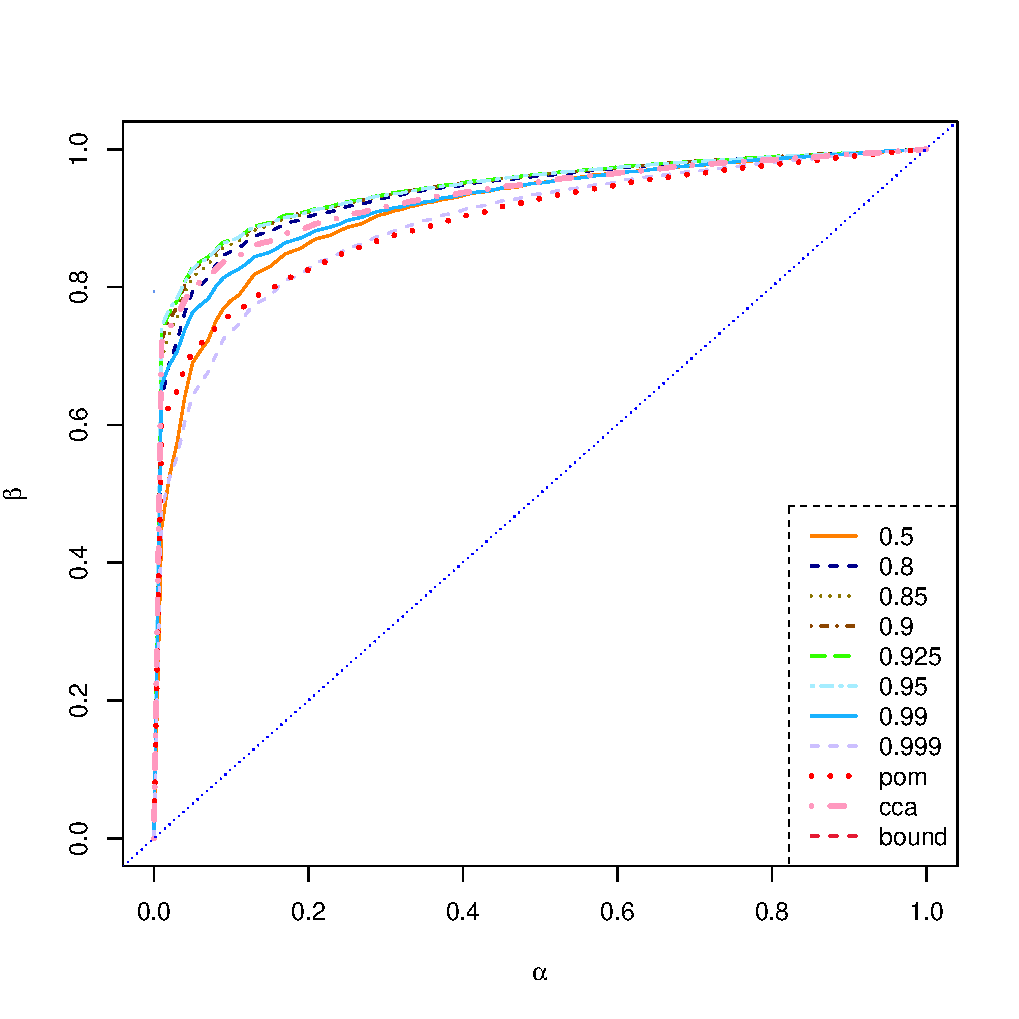
\includegraphics[scale=0.35]{MVN-FC-Tradeoff-OOSc0-01-n150.pdf}
\caption{Power ($\beta$) vs Type I error ($\alpha$) plot for different $w$ values for the Gaussian setting (noisy case)}
\label{fig:MVN-c001-power-alpha}
\end{figure}

\begin{figure}
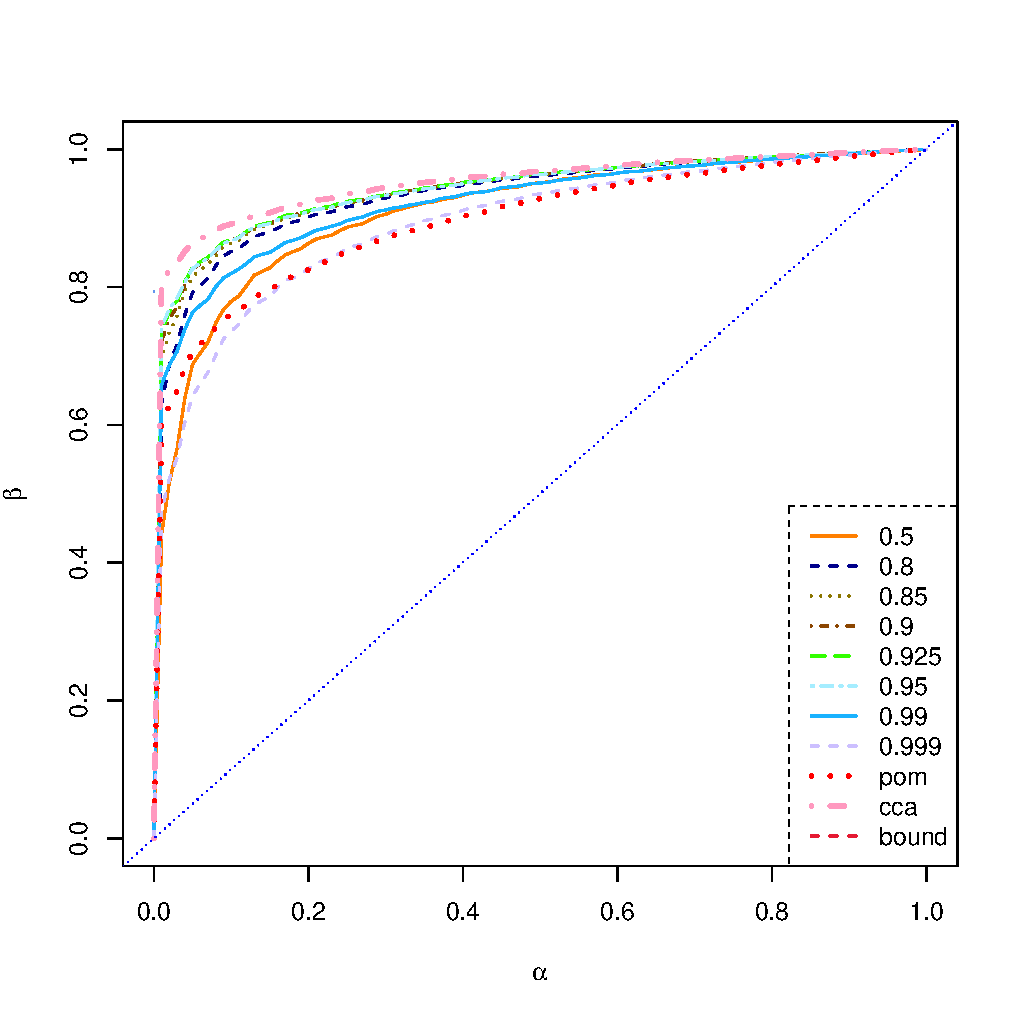
\includegraphics[scale=0.35]{MVN-FC-Tradeoff-OOSc0-n150.pdf}
\caption{Power ($\beta$) vs Type I error ($\alpha$) plot for different $w$ values for the Gaussian setting (noiseless case)}
\label{fig:MVN-c0-power-alpha}
\end{figure}

\begin{figure}
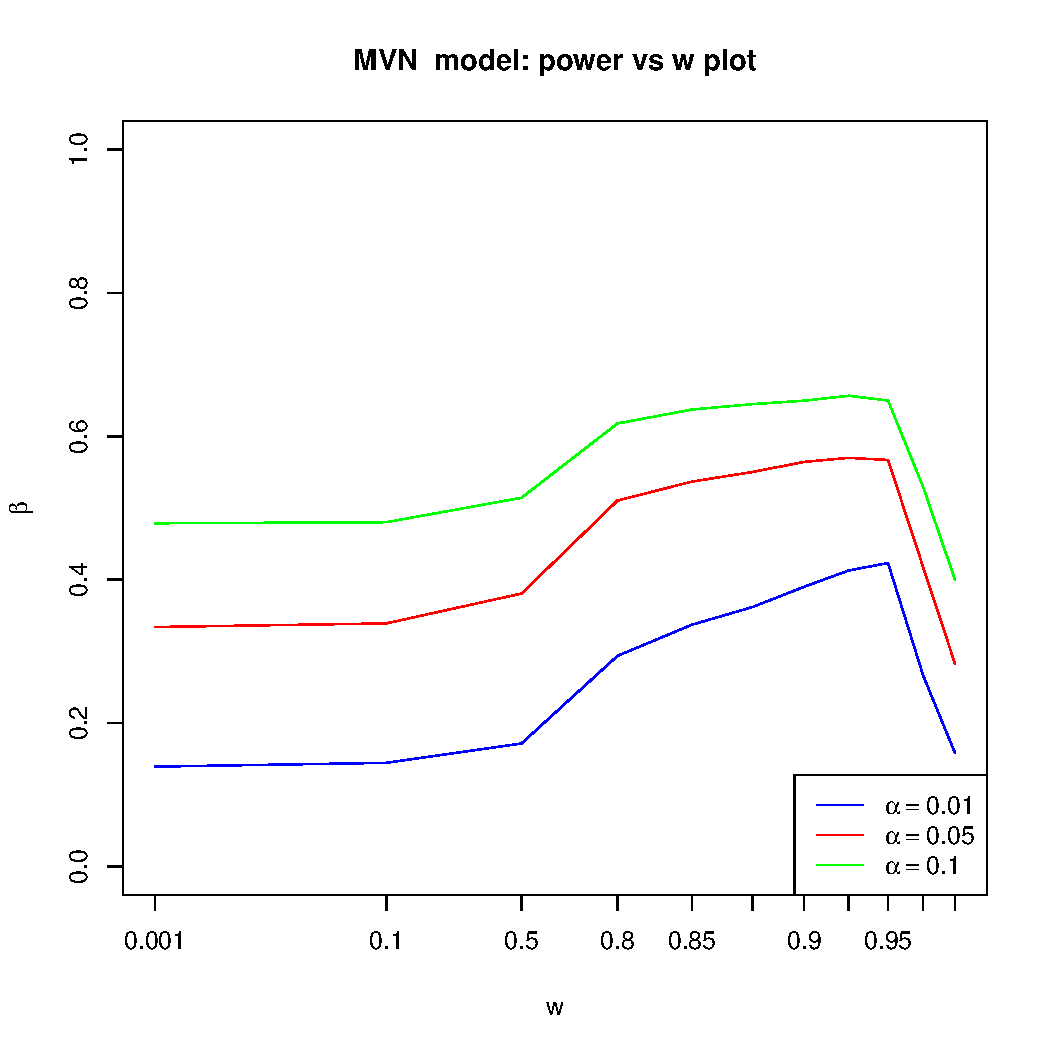
\includegraphics[scale=0.95]{OOS-MVN-power-w-c0-01.pdf}
\caption{Power ($\beta$) vs $w$ plot for different Type I error ($\alpha$) values for the Gaussian setting (noisy case)}
\label{fig:MVN-c001-power-w}
\end{figure}


\begin{figure}
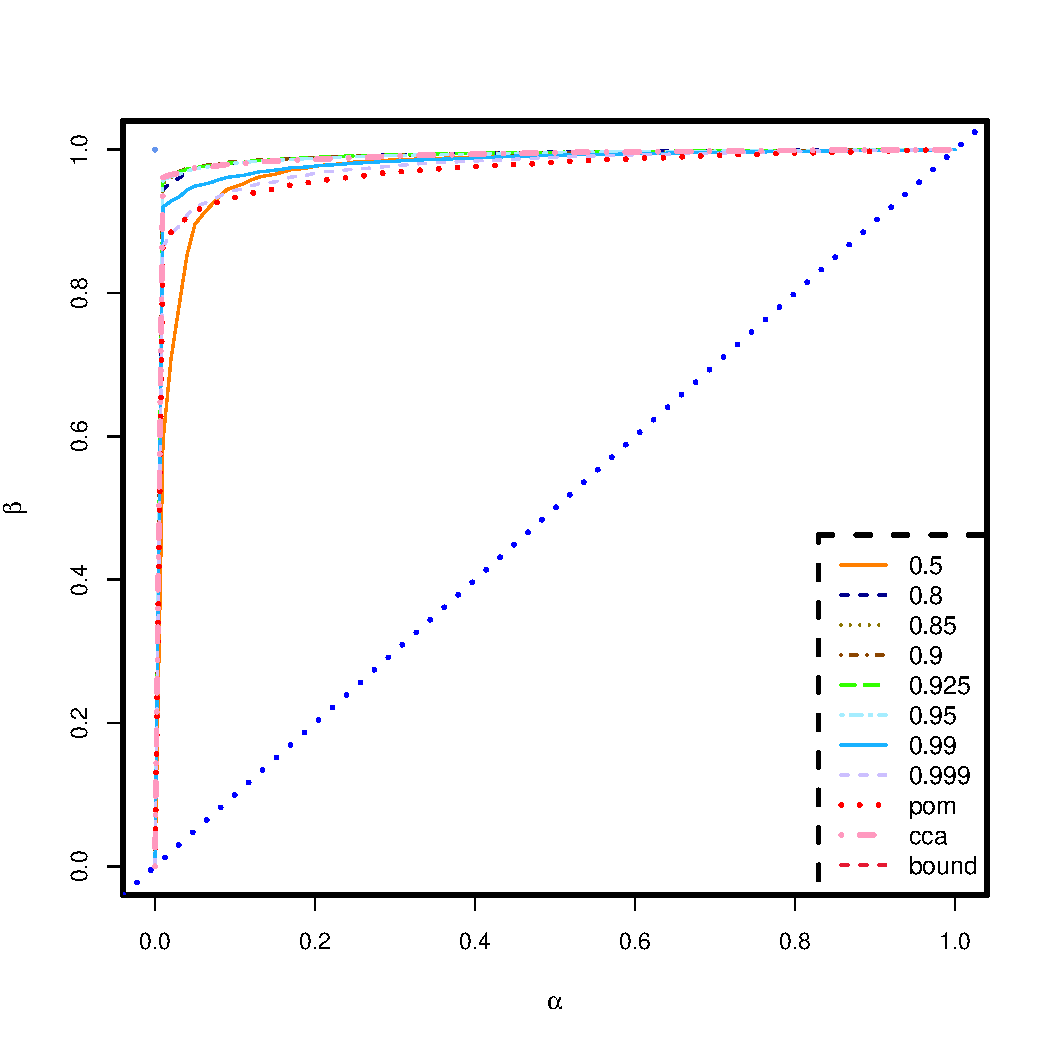
\includegraphics[scale=0.35]{Dirichlet-FC-Tradeoff-OOSc0-01-n150.pdf}
\caption{Power ($\beta$) vs Type I error ($\alpha$) plot for different $w$ values for the Dirichlet setting (noisy case)}
\label{fig:Dir-c001-power-alpha}
\end{figure}

\begin{figure}
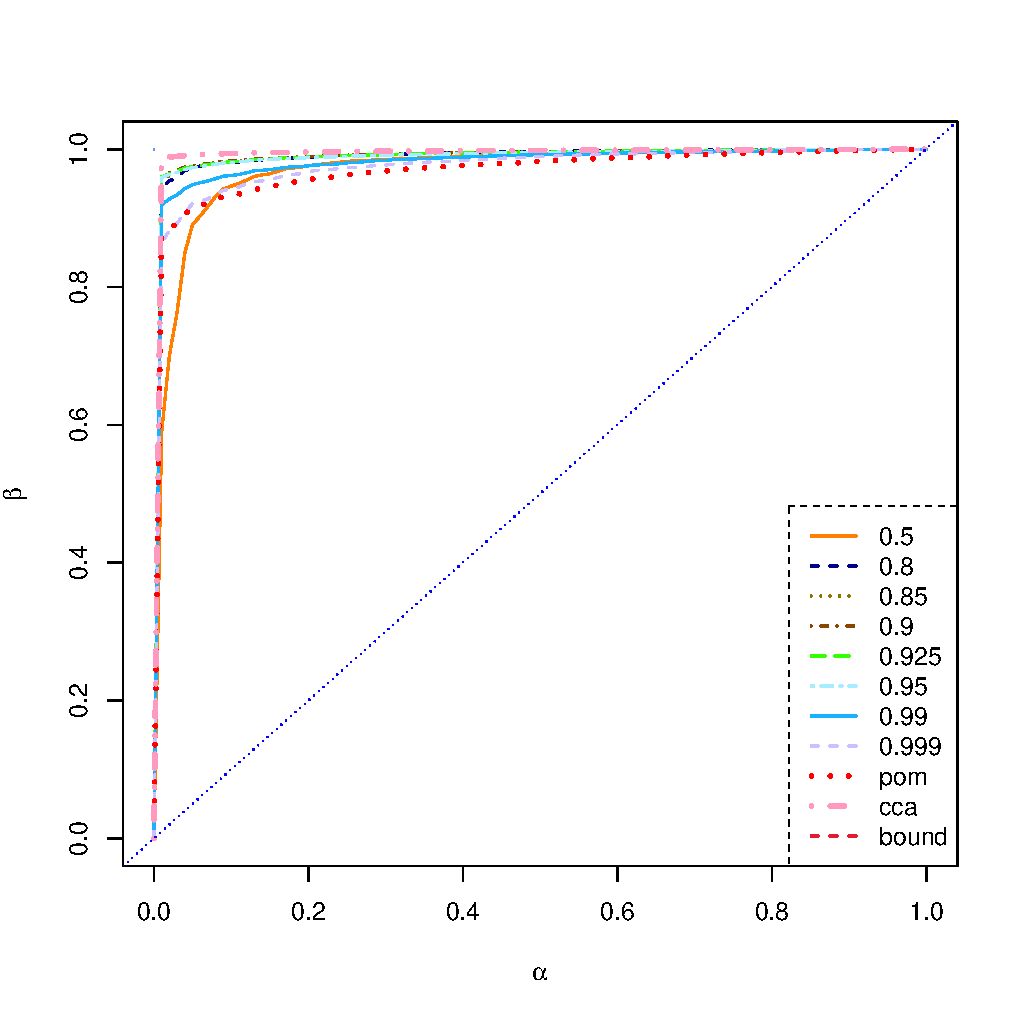
\includegraphics[scale=0.35]{Dirichlet-FC-Tradeoff-OOSc0-n150.pdf}
\caption{Power ($\beta$) vs Type I error ($\alpha$) plot for different $w$ values for the Dirichlet setting (noiseless case)}
\label{fig:Dir-c0-power-alpha}
\end{figure}

\begin{figure}
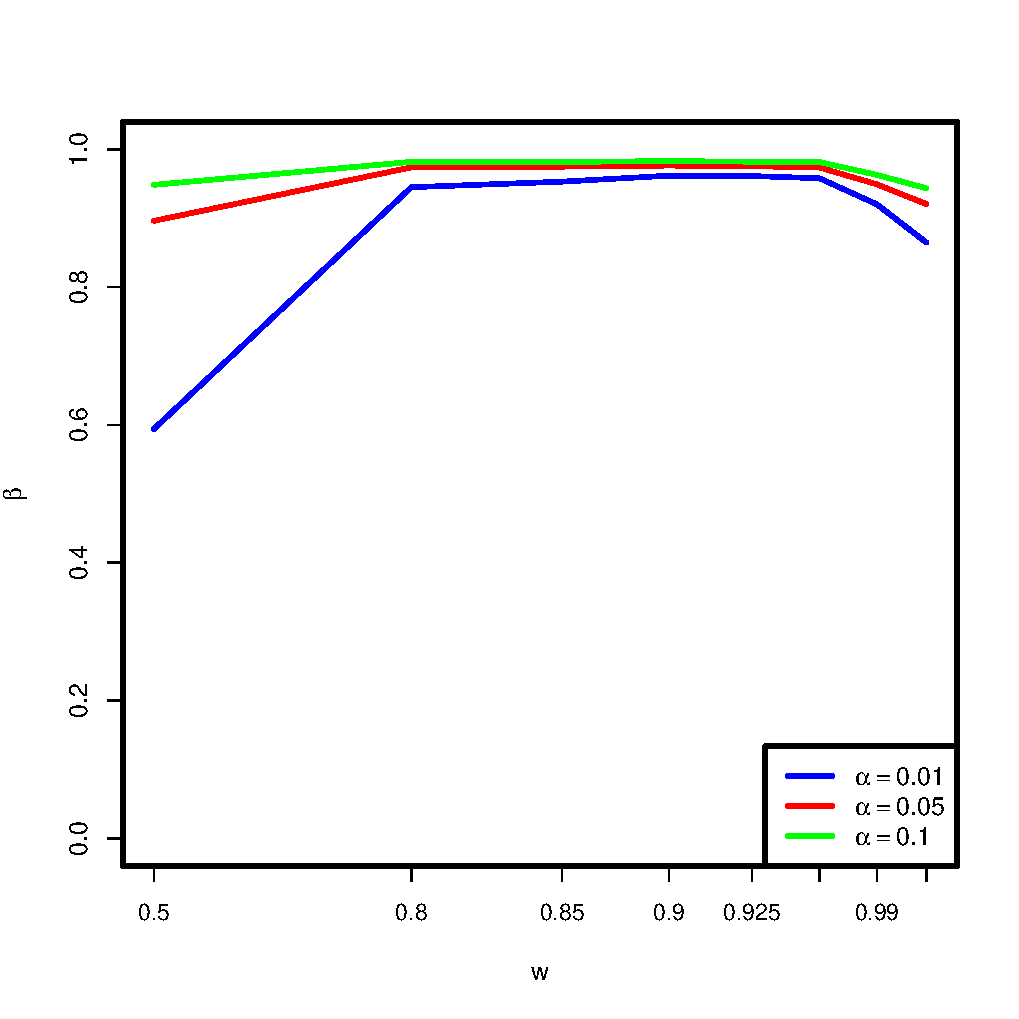
\includegraphics[scale=0.95]{OOSDirichlet-power-w-c0-01.pdf}
\caption{Power ($\beta$) vs $w$ plot for different Type I error ($\alpha$) values for the Gaussian setting (noisy case)}
\label{fig:MVN-c001-power-w}
\end{figure}

Setting p and q to 5 and 10, respectively, for $n=150$ and $m=150$, the average of the power values for $nmc=150$ Monte Carlo replicates are computed at  different $\alpha$s and are plotted in Figure \ref{fig:MVN-c001-ROC} against $\alpha$ for the Gaussian setting.  Qualititatively similar plots for the Dirichlet setting  exist.  The plot in Figure \ref{fig:MVN-c001-ROC} shows that for different values of  $w$, we have varying power curves, and some $w$ values outperform others in terms of power. In Figure \ref{fig:MVN-c001-beta-w},  $\beta(w)$ is plotted against $w$ for fixed values of $\alpha$. It is  interesting that the optimal value of $w$ seems to be in the range of $(0.85,1)$ for all settings, which suggests commensurability might be more critical for our hypothesis testing task. 




\begin{comment}
\begin{figure}
\includegraphics[scale=0.35]{OOS-MVN-power-w-c0.pdf}
\caption{$\beta$ vs $w$ plot for fixed $\alpha$ values for the Gaussian setting (noiseless case)}
\label{fig:MVN-c0-beta-w}
\end{figure}
\end{comment}

\begin{figure}
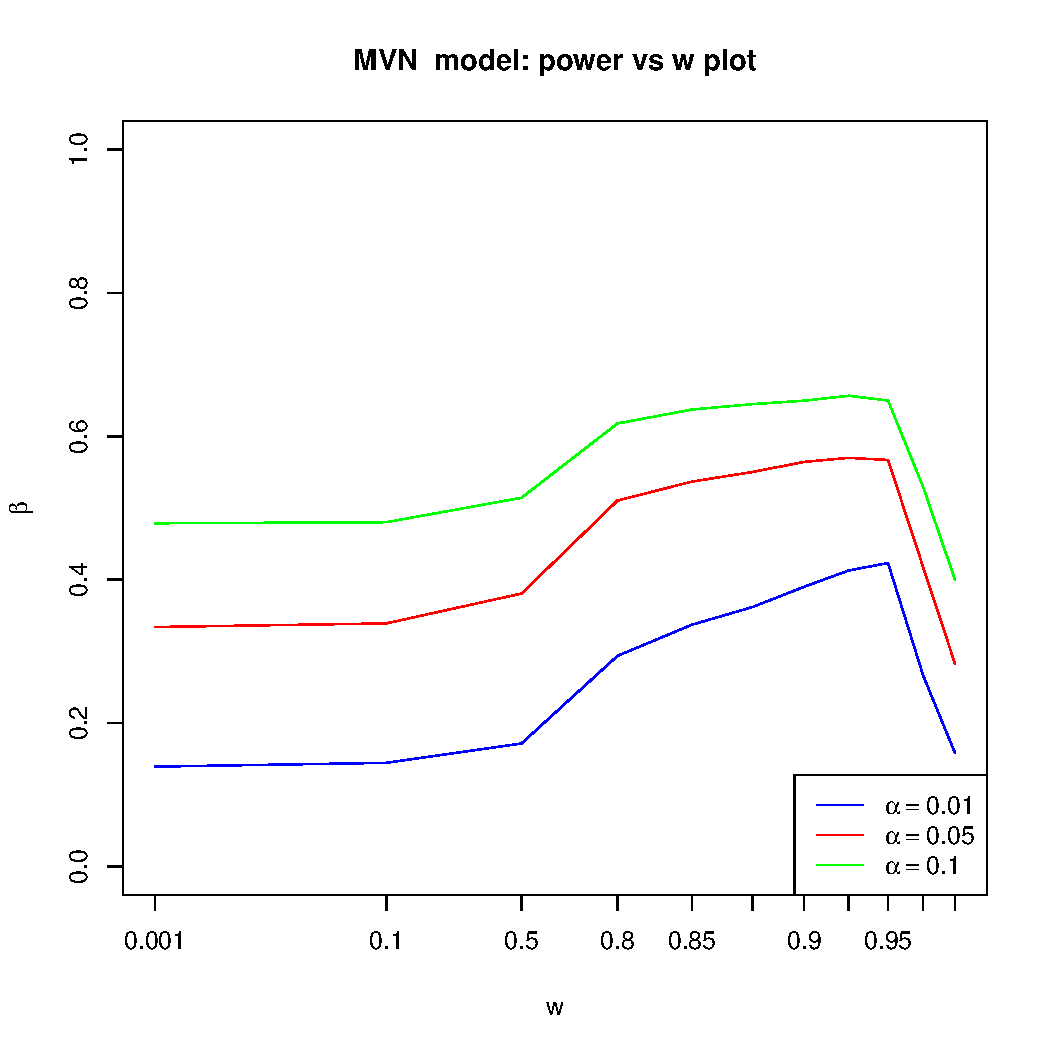
\includegraphics[scale=0.65]{OOSMVN-power-w-c001.pdf}
\caption{Power ($\beta$) vs $w$ plot for fixed Type I error ($\alpha$) values for the Gaussian setting (noisy case)}
\label{fig:MVN-c001-beta-w}
\end{figure}
Note that in Figure \ref{fig:MVN-c001-beta-w} for $\alpha=0.05$, $\beta_{\alpha=0.05}(w=0.99)\geq\beta_{\alpha=0.05}(w=0.5)$. However, for $\alpha=0.2$, $\beta_{\alpha=0.2}(w=0.99)\leq\beta_{\alpha=0.2}(w=0.5)$. This justifies our comment that  $w^{*}$  must be defined with respect to $\alpha$.


\begin{comment}
\begin{figure}
\includegraphics[scale=0.35]{OOS-Dirichlet-power-w-c0.pdf}
\caption{$\beta$ vs $w$ plot for fixed $\alpha$ values for the Dirichlet setting(noiseless case)}
\label{fig:fig7}
\end{figure}

\begin{figure}
\includegraphics[scale=0.35]{OOS-Dirichlet-power-w-c0-01.pdf}
\caption{$\beta$ vs $w$ plot for fixed $\alpha$ values for the Dirichlet setting(noisy case)}
\label{fig:fig8}
\end{figure}
\end{comment}



Note that  for all of the settings, the estimate of the optimal $w^{*}$ has  higher power than $w$=0.5 (the unweighted case).
To test the statistical significance of this observation, we wish to test the null hypothesis that  $H_{0}: \beta_{\alpha}({\hat{w}^*})\leq\beta_{\alpha}({w=0.5})$ against the alternative $H_{A}=\beta_{\alpha}({\hat{w}^*})>\beta_{\alpha}({w=0.5})$.  The least favorable null hypothesis is that  $H_{0}: \beta_{\alpha}({\hat{w}^*})=\beta_{\alpha}({w=0.5})$.

For a fixed $\alpha$ value, one can compute two critical values  using the test statistic values for the two $w$ values that are being compared. Using these critical  values, we can  determine the decision made by each test for each pair of embedded points, $(\tilde{y}_i^{(1)},\tilde{y}_i^{(2)}),\hspace{7pt}i=1,\ldots,m$. To compare the  two statistical tests with different $w$ values, one can prepare a $2\times 2$ contingency-table of correct decisions and incorrect decisions made by each statistical test (or equivalently true and false classifications made by two classifiers). Denote decision outcome as $c_1$ for the first statistical test and $c_2$ for the second statistical test. If $c_1=True$ and $c_2=False$ for an instance,  the first test made the correct decision and the second test made the incorrect decision with regard to the null and alternative hypotheses.
% McNemar's test was used to compare the two contingency tables for fixed $\alpha$. McNemar's test is a statistical test for %comparing two binary classifiers based on a 2-by-2 table of the counts of misclassifications of each. That is,
Consider the contingency table for a Monte Carlo replicate given by $$G^{(l)}= \begin{array}{|c|c|}
      \hline
       e_{FF}^{(l)} & e_{TF}^{(l)}\\
      \hline
       e_{FT}^{(l)} & e_{TT}^{(l)}\\
      \hline
      \end{array}      $$  where $l$ is the index of the MC replicate, $e_{c_1c_2}^{(l)}$ is equal to the number of instances at which the true hypothesis were identified  correctly ($c_1=True$) or incorrectly ($c_1=False$) by the first test, and correctly ($c_2=True$) or incorrectly ($c_2=False$) by the second test in that MC replicate.

Under the null  hypothesis, $Pr[\left(c_1c_2\right)=(TF)]=Pr[\left(c_1c_2\right)=(FT)]$, so $\sum_l{I \{e_{TF}^{(l)}>e_{FT}^{(l)}\}}$ will be distributed according to  the binomial distribution, $\mathcal{B}(nmc,0.5)$. ($I\{\cdot\}$ is the indicator function.) 

% For each Monte Carlo replicate, the p-value of McNemar's test was computed separately.

\begin{comment}
\begin{figure}
\begin{tabular}{p{4.7cm}p{4.7cm}}
$e_{00}$:Misclassified by \newline Both C1 and C2 & $e_{10}$:Correctly Classified by C1,\newline Misclassified by C2\\
& \\
$e_{01}$:Correctly Classified by C1, \newline Misclassified by C2 & $e_{11}$:Correctly Classified by \newline Both C1 and C2
\end{tabular}. 

\caption{Contingency Table for McNemar's test for comparing two classifiers, C1 and C2}
\label{fig:cont-table}
\end{figure}
\end{comment}

For the noisy version of the Gaussian setting at allowable type I error 0.05 for the two tests, when comparing  the null hypothesis that  $H_{0}: \beta_{\alpha}({\hat{w}^*})=\beta_{\alpha}({w=0.5})$ against the alternative $H_{A}=\beta_{\alpha}({\hat{w}^*})>\beta_{\alpha}({w=0.5})$, we find $p<1.09E-24$ which indicates the power using estimate of optimal $w^*$ is significantly greater than the power when using $w=0.5$. 
%In fact
% the distribution of p-values from McNemar's tests is skewed and  we reject $\beta_{0.5}>=\beta_{w^*} $ for  55\%  of the %Monte Carlo replicates.





Setting p and q to 5 and 10, respectively, for $n=150$ and $m=150$, the average of the power values for $nmc=150$ Monte Carlo replicates are computed at  different $\alpha$s and are plotted in Figure \ref{fig:MVN-c001-ROC} against $\alpha$ for the Gaussian setting.  Qualititatively similar plots for the Dirichlet setting  exist.  The plot in Figure \ref{fig:MVN-c001-ROC} shows that for different values of  $w$, we have varying power curves, and some $w$ values outperform others in terms of power. In Figure \ref{fig:MVN-c001-beta-w},  $\beta(w)$ is plotted against $w$ for fixed values of $\alpha$. It is  interesting that the optimal value of $w$ seems to be in the range of $(0.85,1)$ for all settings, which suggests commensurability might be more critical for our hypothesis testing task. 

The same pair of plots are included for various values of parameters $p$,$q$ ,$r$ and $c$.






\section{The general case of more than two conditions}


As it was mentioned, all of the approaches are generalizable to $K>2$ conditions, though some ambiguities need to be resolved. For example,  the alternative hypothesis could be  defined as the event that at least one of the K new dissimilarities are pairwise unmatched ($ H_{A1}: \exists i, j , 1\leq i < j \leq K :\bm{y}_{i} \nsim \bm{y}_{j} $ ) or it could be defined as the case that absolutely none of the K dissimilarities are matched   ($H_{A2}: \forall i, j , 1\leq i < j \leq K :\bm{y}_{i} \nsim \bm{y}_{j}$ )  .
% and the sample from the alternative must be generated accordingly during Monte Carlo simulation. In the first case, an appropriate test statistic is then the maximum of the pairwise %distances between embeddings of each test K-tuple.

For PoM, one can use Procrustes analysis  generalized to more than two configurations. Generalized Procrustes Analysis \cite{GPCA} is a well established method for finding a collection of linear transformations that minimizes the mismatch between the transformed configurations and a "mean`` shape computed from these configurations. 

For CCA, there are multiple generalizations available as the correlation between more than two configurations can be defined in multiple ways \cite{generalCCA}. Let $X_1,\ldots,X_K$ be random vectors. Consider the first set of canonical variates to be computed, $Z_1^{1},\ldots,Z_K^{1}$. Denote  the correlation matrix of  $Z_1^{1},\ldots,Z_K^{1}$ by $\Phi^{(1)}$.   The following three criteria  are proposed in \cite{generalCCA}.
\begin{itemize}
\item SUMCOR. Maximize the sum of the elements of $\Phi^{(1)}$ : $\mathbf{1'}(\Phi^{(1)})\mathbf{1'}$
\item MAXVAR. Maximize the largest eigenvalue of $\Phi^{(1)}$ : $\lambda^{(1)}_1$ 
\item  MINVAR. Minimize  the smallest eigenvalue of $\Phi^{(1)}$ : $\lambda^{(m)}_1$ 
\end{itemize}
One can think of all of these criteria as different norms on the correlation matrix.
%For $H_{A1}$ MINVAR might be a good choice, since the exploitation task is to find evidence against the null and as favorable to the alternative as possible. 
%MINVAR should be small whenever there exists \emph{at least} one unmatched measurement so under the alternative hypothesis. MAXVAR, in this case, wouldn't be necessarily small under alternative with respect to null.  MINVAR statistic should be stochastically smaller compared to null distribution. For $H_{A2}$ MAXVAR is appropriate, since under the alternative hypothesis, MAXVAR should be very small compared to under the null hypothesis. 
%For $H_{A2}$ MAXVAR is appropriate, since under the alternative hypothesis, MAXVAR should be very small compared to under the null hypothesis. It is quite possible the other generalizations are appropriate for our task.
An interesting question is whether any of these generalizations is more appropriate for $H_{A1}$ or $H_{A2}$.

A multivariate normal model with $K=3$ conditions were used to generate $K$-condition matched data. 
The simulations in the previous section\ref{sec:Simulation Results} were repeated with this $K$-condition data. 
The alternative was chosen as $ H_{A1}$ and SUMCOR was chosen as the generalization of CCA.
 $q$-dimensional noise vectors of magnitude $c$ were added to the matched measurements. 
 The ROC curves for these simulations are shown in \ref{fig:MVN-c001-ROC-Kcond}.


 



